\chapter{Experiments}
This section shows the results of the experiments done with the
implemented solutions. 

The methods were tried with volumes to which artificial differences of
distinct sizes and shapes were added; and also with real patient's
volumes obtained from the Uppsala University Hospital.


\section{Experiments Conditions}

\subsection{Artificial Differences}
For this experiments, the MRIs used belong to a healthy patient and
the time difference between each exam is very short, so it is expected
of them to have no changes.

First, the methods were used on three distinct sizes of differences:
large, medium and small; each of which represents volume loss. The
considered sizes are based on the comparisons done with real patients
and the sizes of the differences presented on those cases.

Finally, the last artificial experiment was done by increasing the size
of a small area of the brain, in order to represent movement or change
of size of an area inside the brain.


\subsection{Real Differences}
For this experiment, the MRIs from three real patients with known
differences were compared using both methods.

Two of them are patients of the study for which this project was
started, and so they have very small differences that are hard to
detect with the naked eye.

The third patient has larger known differences produced by a medical
condition and its subsequent surgery.


\section{Artificial Differences Results}
The initial baseline volume without modifications used for all of the
artificial tests related to volume loss can be seen in the following
image:

\begin{figure}[H]
  \centering
  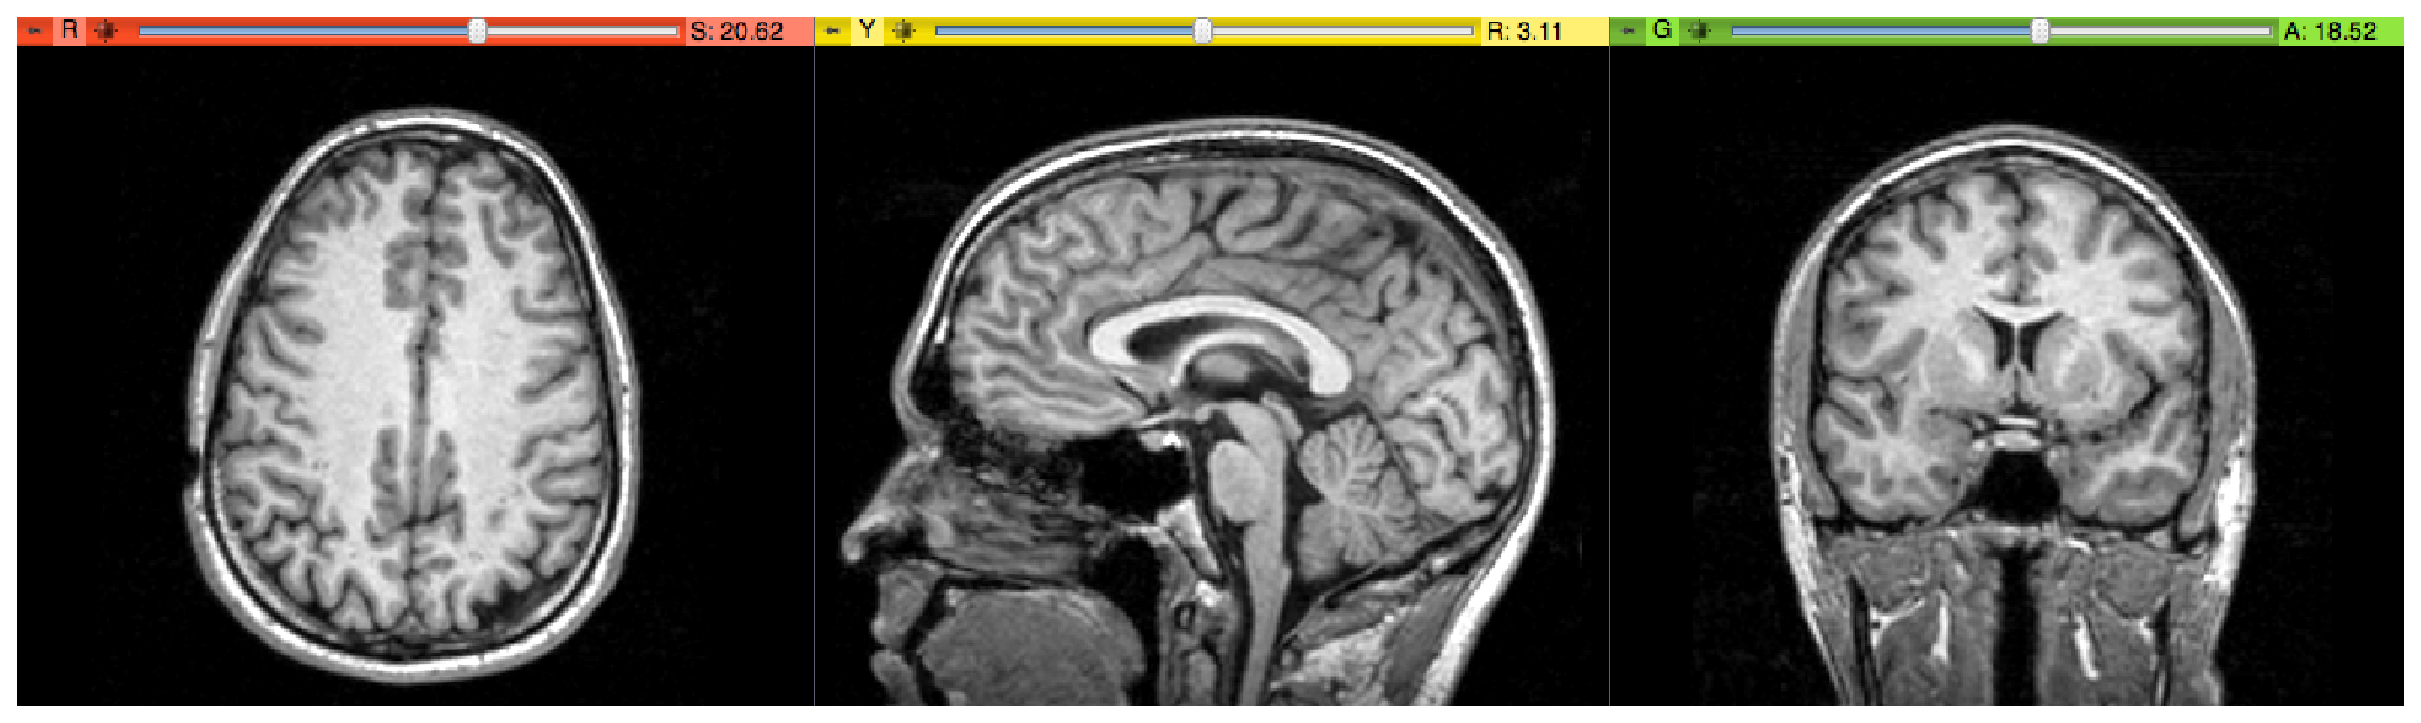
\includegraphics[scale=0.3]{/experiment_bigger/biggerA.eps}
  \caption{Artificial Differences: Baseline volume}
  \label{artificial_base}
\end{figure}

\subsection{Size: Large}
Cubes of large size where deleted from the follow-up volume to
represent areas of volume loss. The following volume was obtained:

\begin{figure}[H]
  \centering
  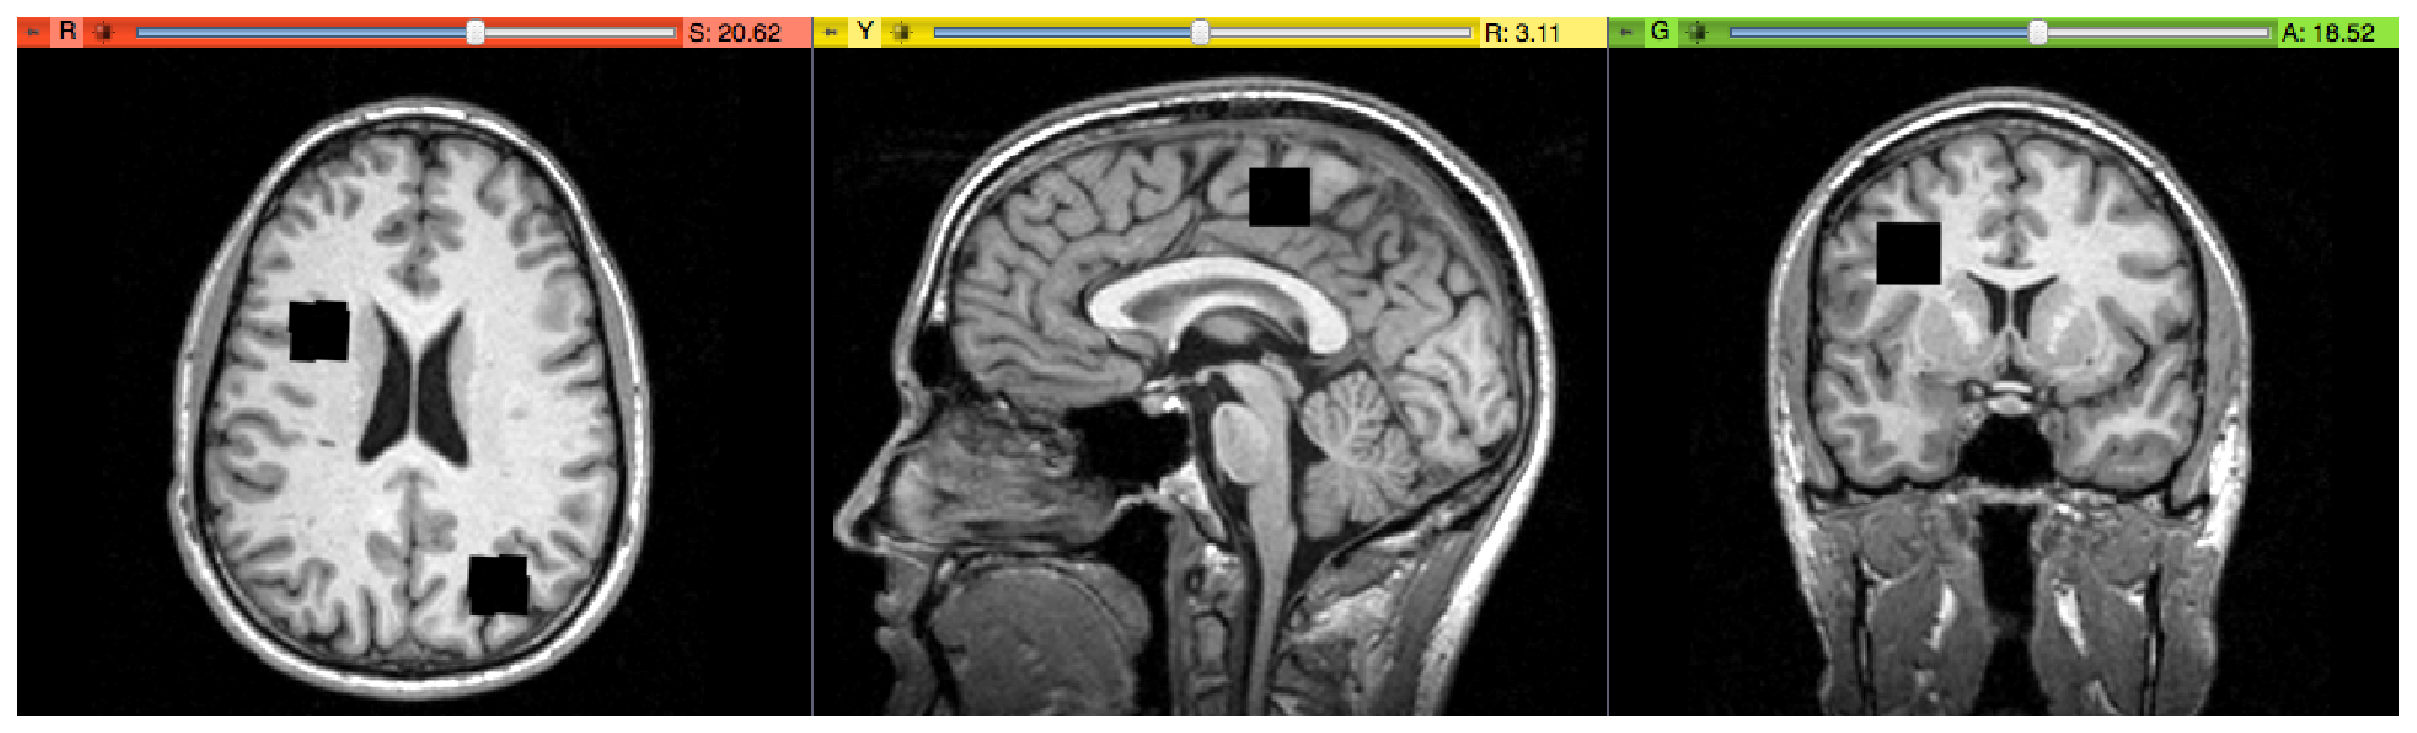
\includegraphics[scale=0.3]{/experiment_bigger/biggerB_subtracted.eps}
  \caption{Large Differences: Modified Follow-up volume}
  \label{largeB}
\end{figure}

\subsubsection{Voxel-based Method}
The result obtained with this method and large differences is pretty
good. All the differences are found and easy to see in the result.

\begin{figure}[H]
  \centering
  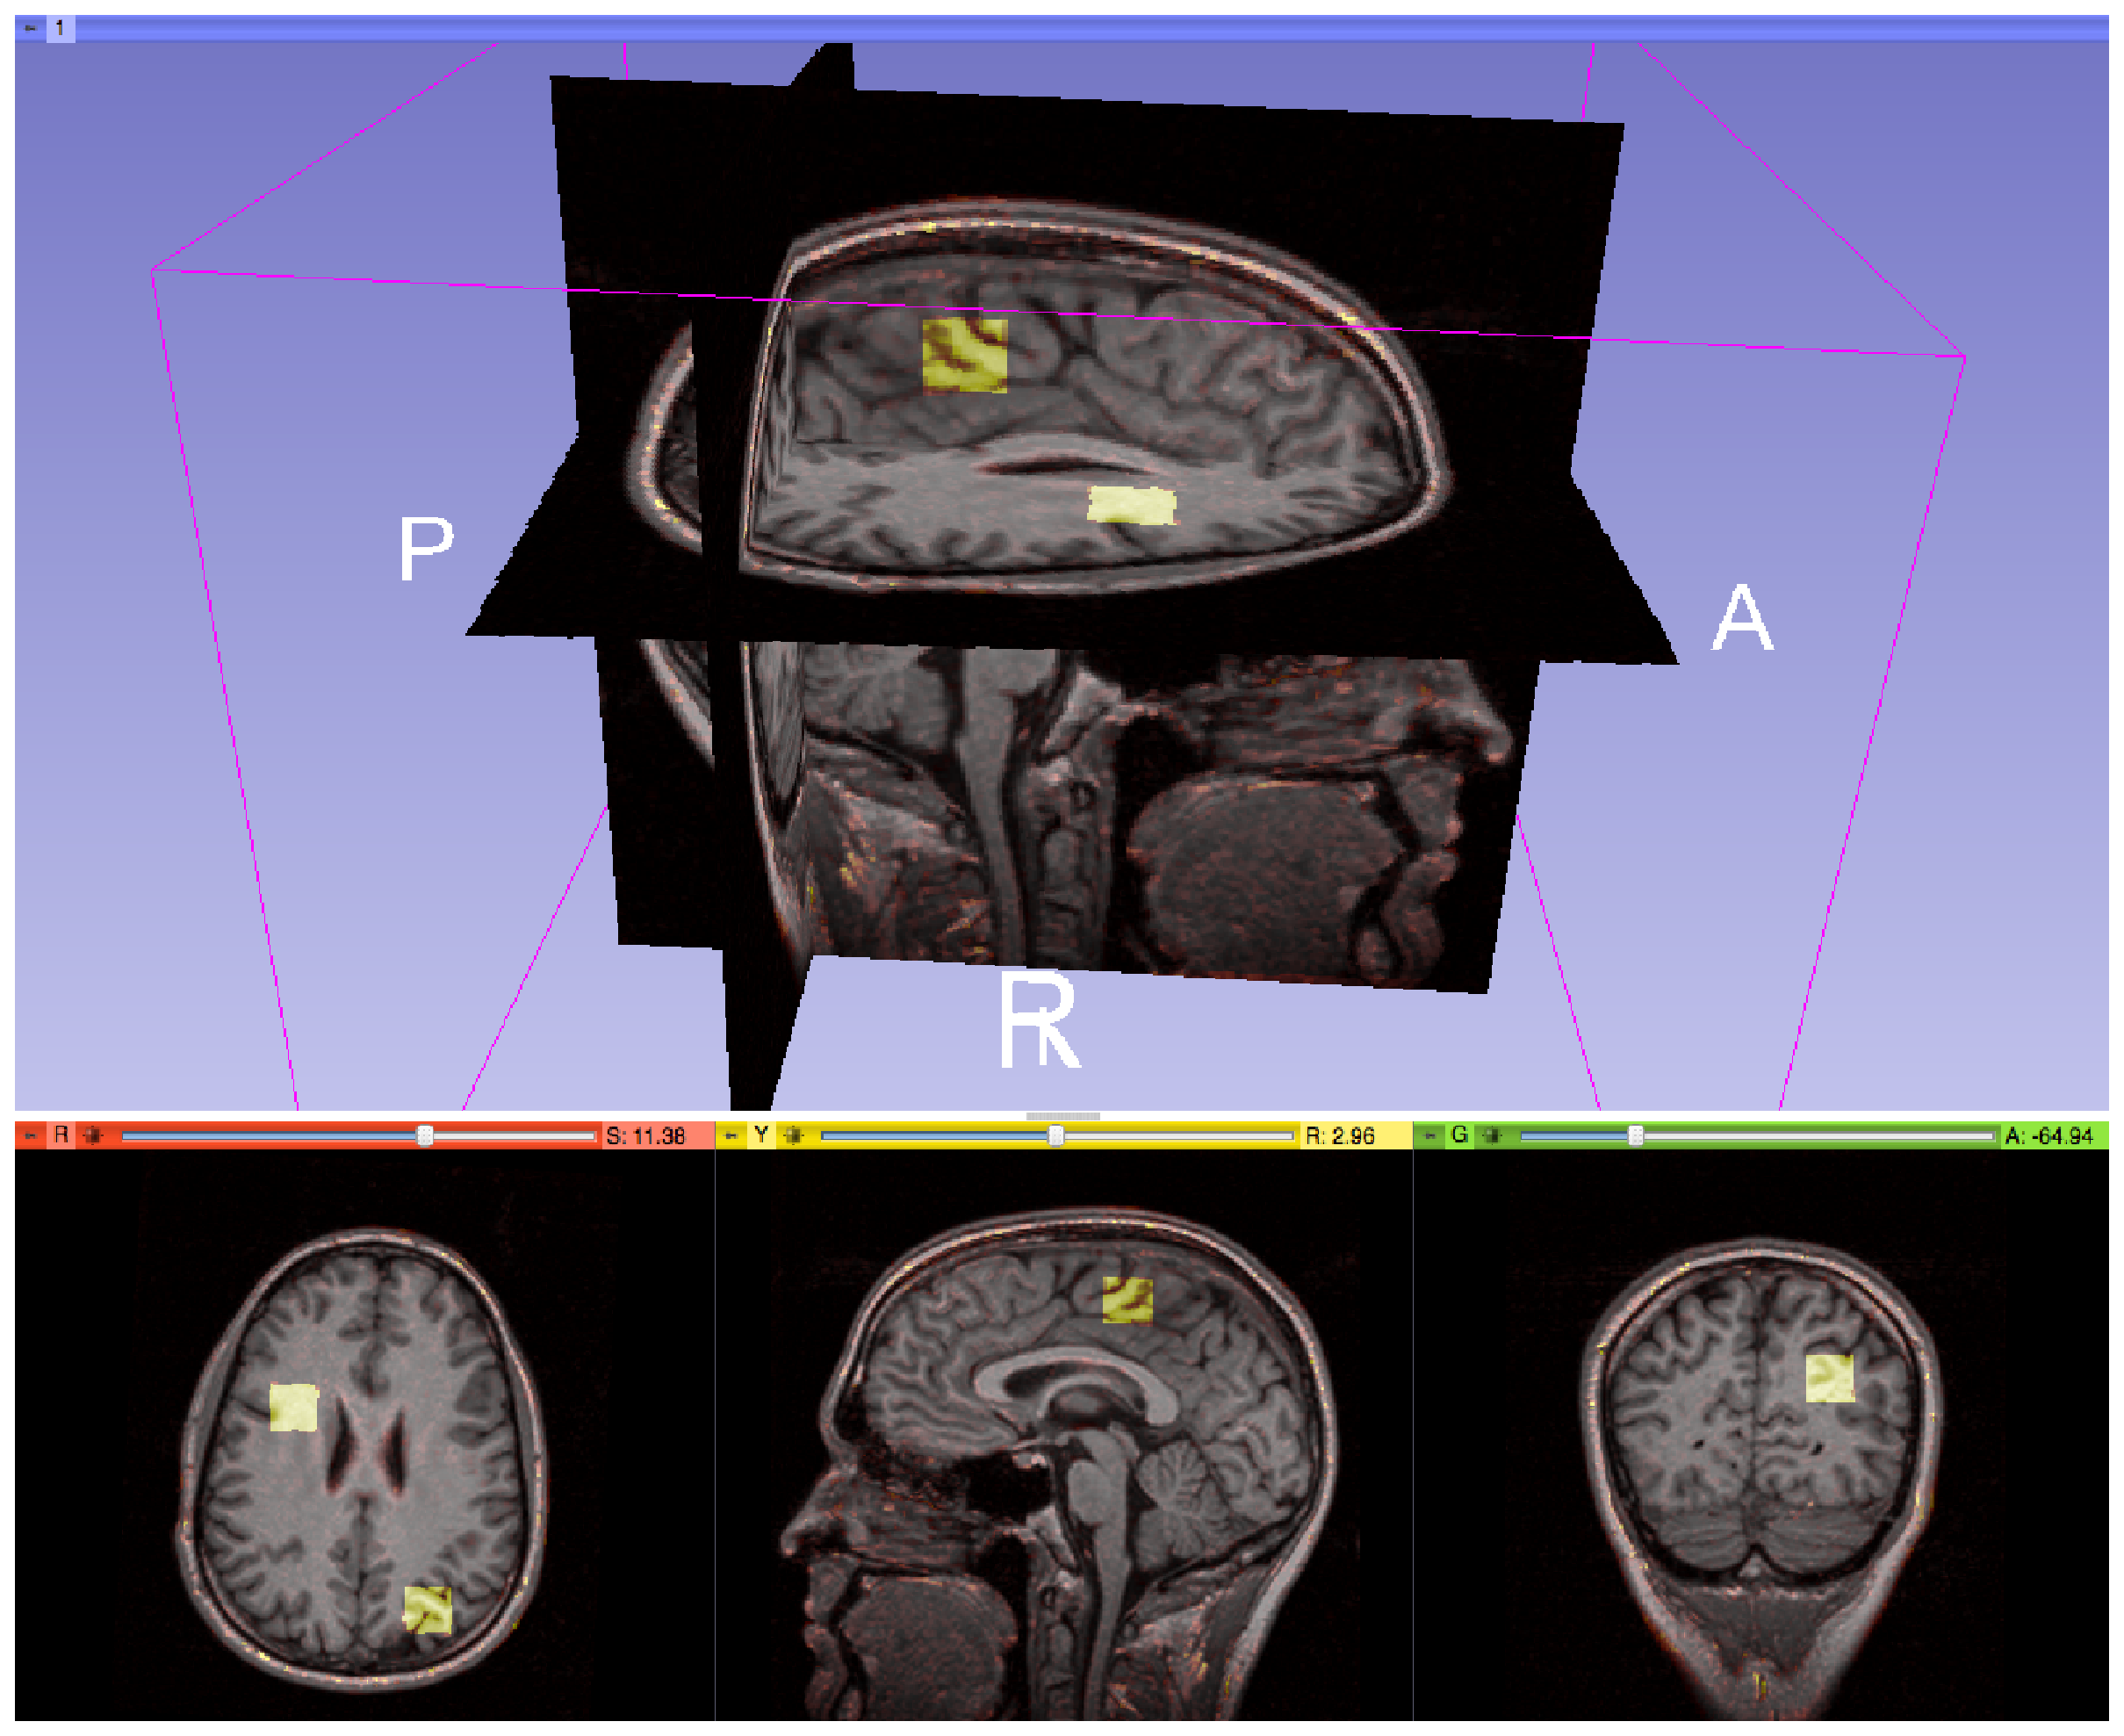
\includegraphics[scale=0.2]{/experiment_bigger/voxel_bigger1.eps}
  \caption{Artificial Large: Voxel-base method}
  \label{voxel_large1}
\end{figure}

Another angle of the result:

\begin{figure}[H]
  \centering
  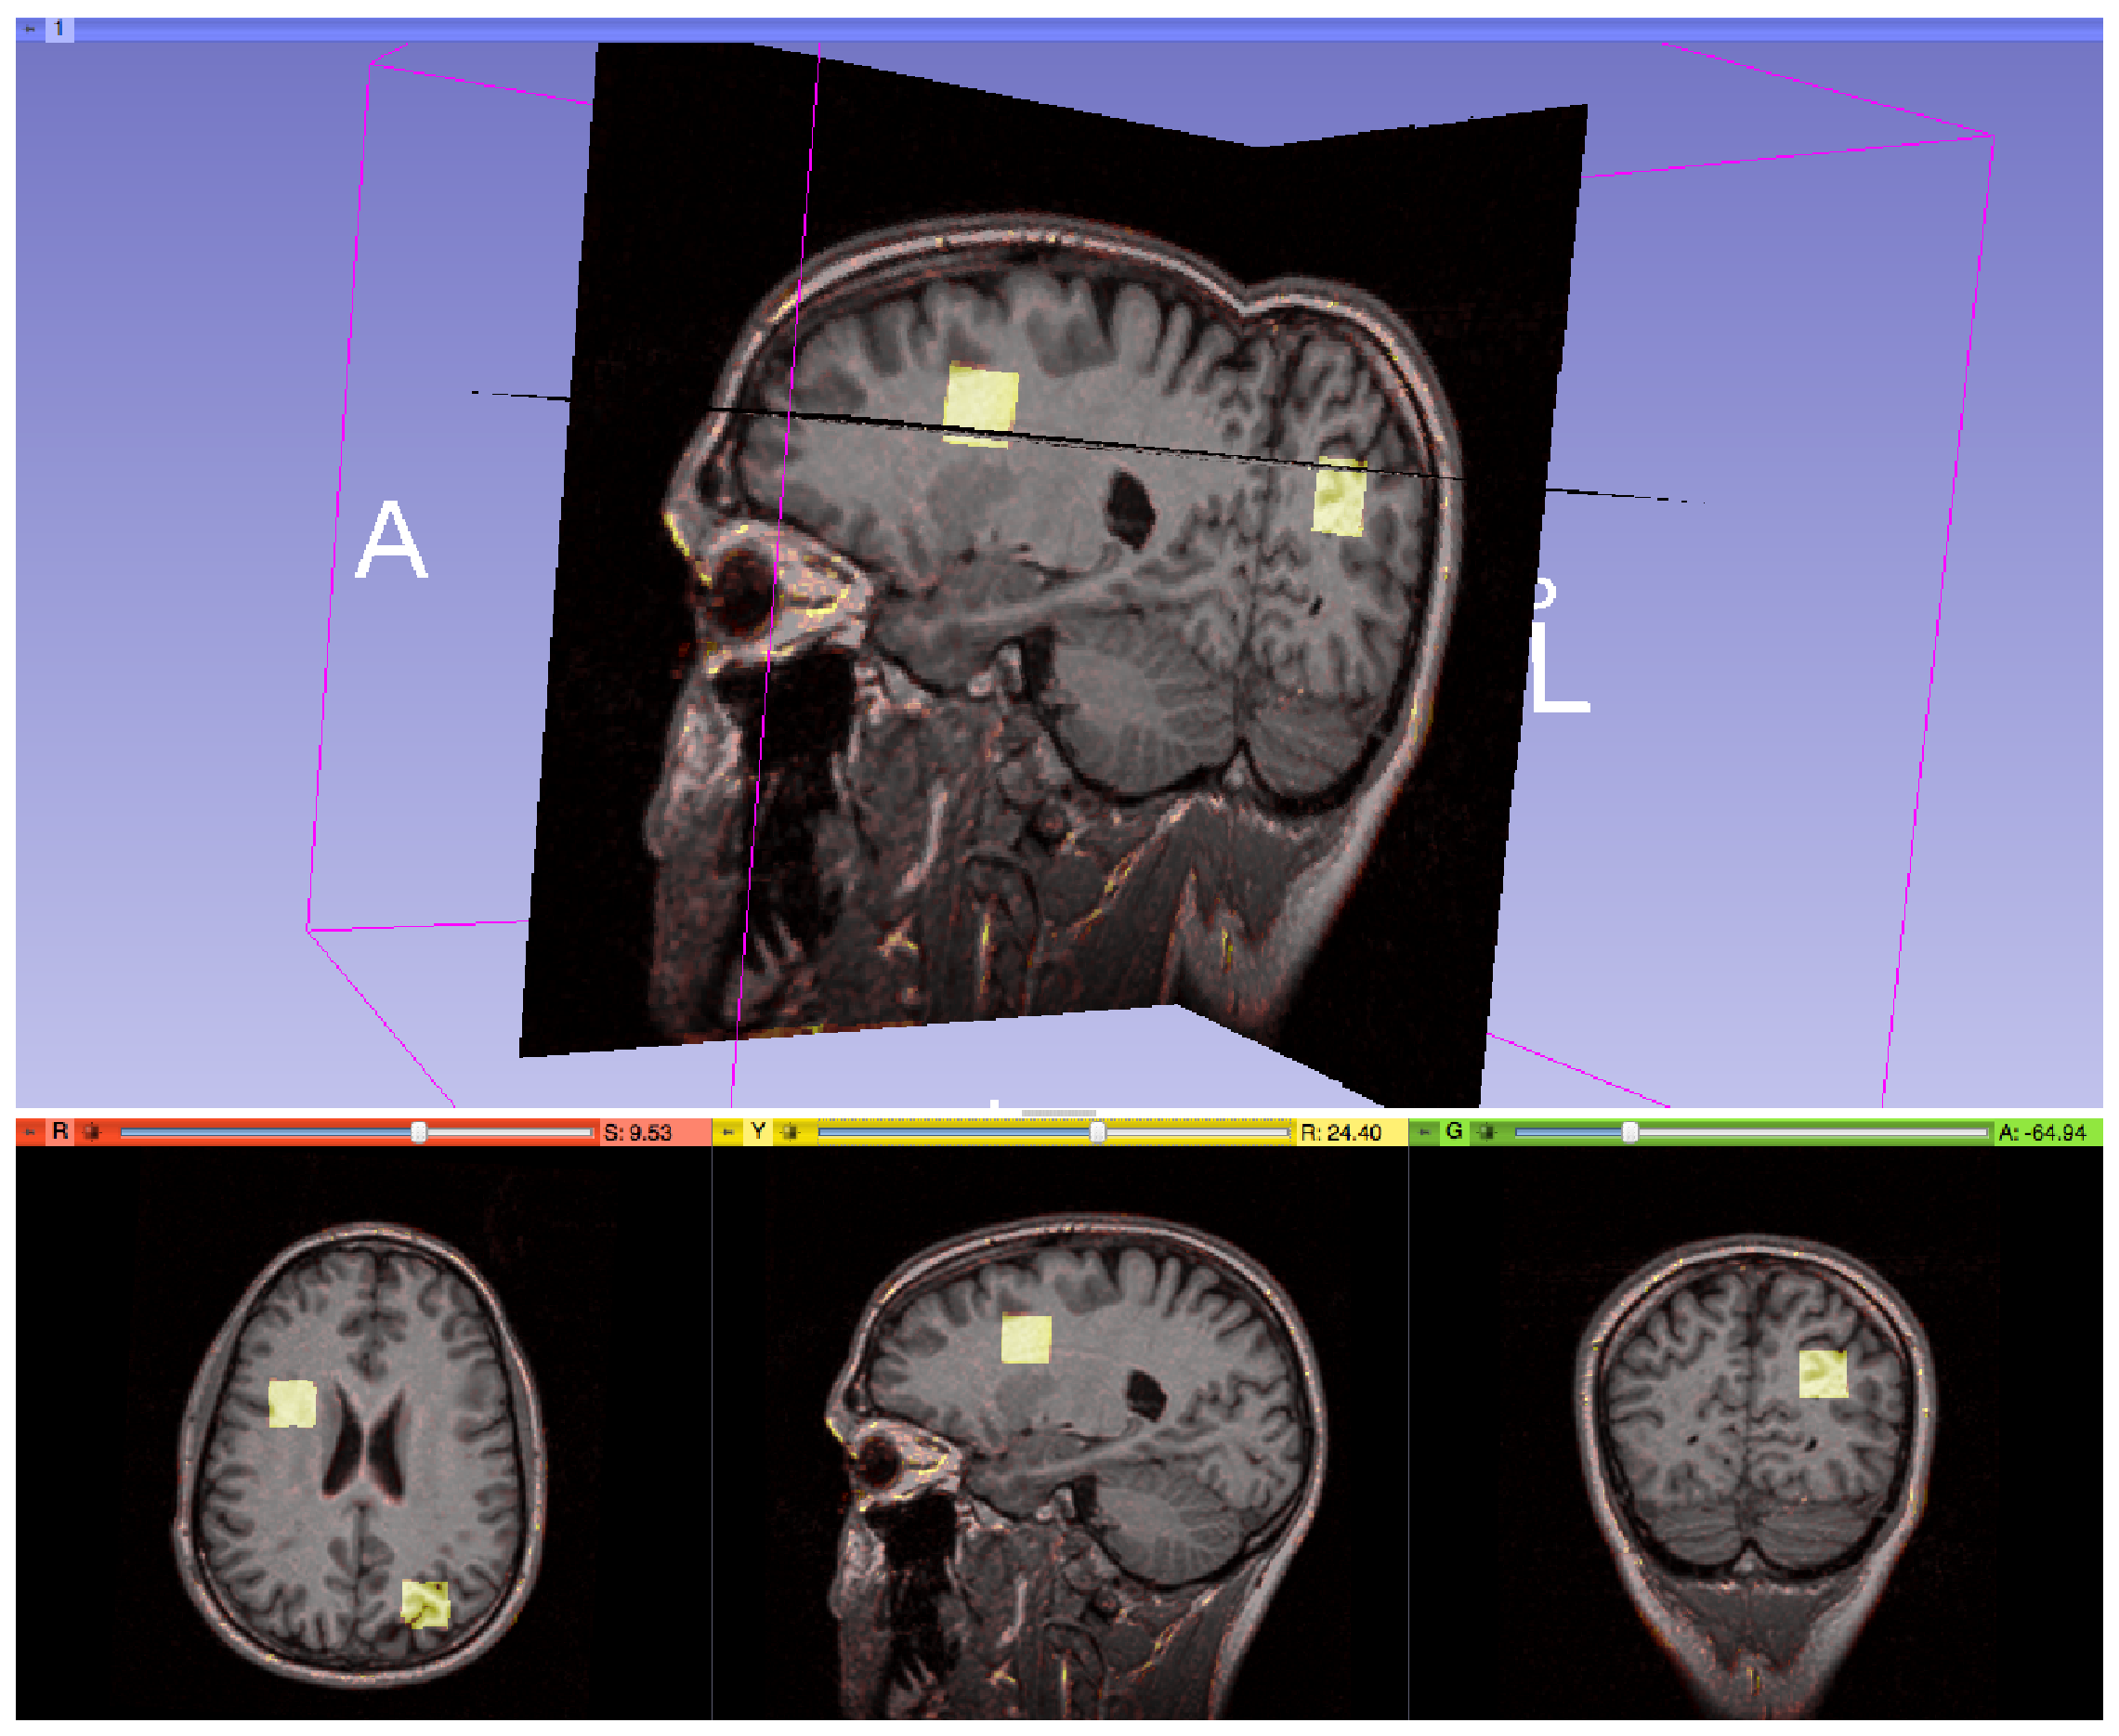
\includegraphics[scale=0.2]{/experiment_bigger/voxel_bigger2.eps}
  \caption{Artificial Large: Voxel-base method}
  \label{voxel_large2}
\end{figure}

\subsubsection{Tensor-based Method}
In the result obtained with this method the differences are easy to
find, but their borders are not properly defined. The method gives the
position of the differences but not their exact shape.

The parameters used to obtain this result are:
\begin{description}
\item \textit{Deformation field smoothing sigma:} 2.5
\item \textit{Shrinkage percentage:} 80
\item \textit{Growth percentage:} 65
\end{description}

\begin{figure}[H]
  \centering
  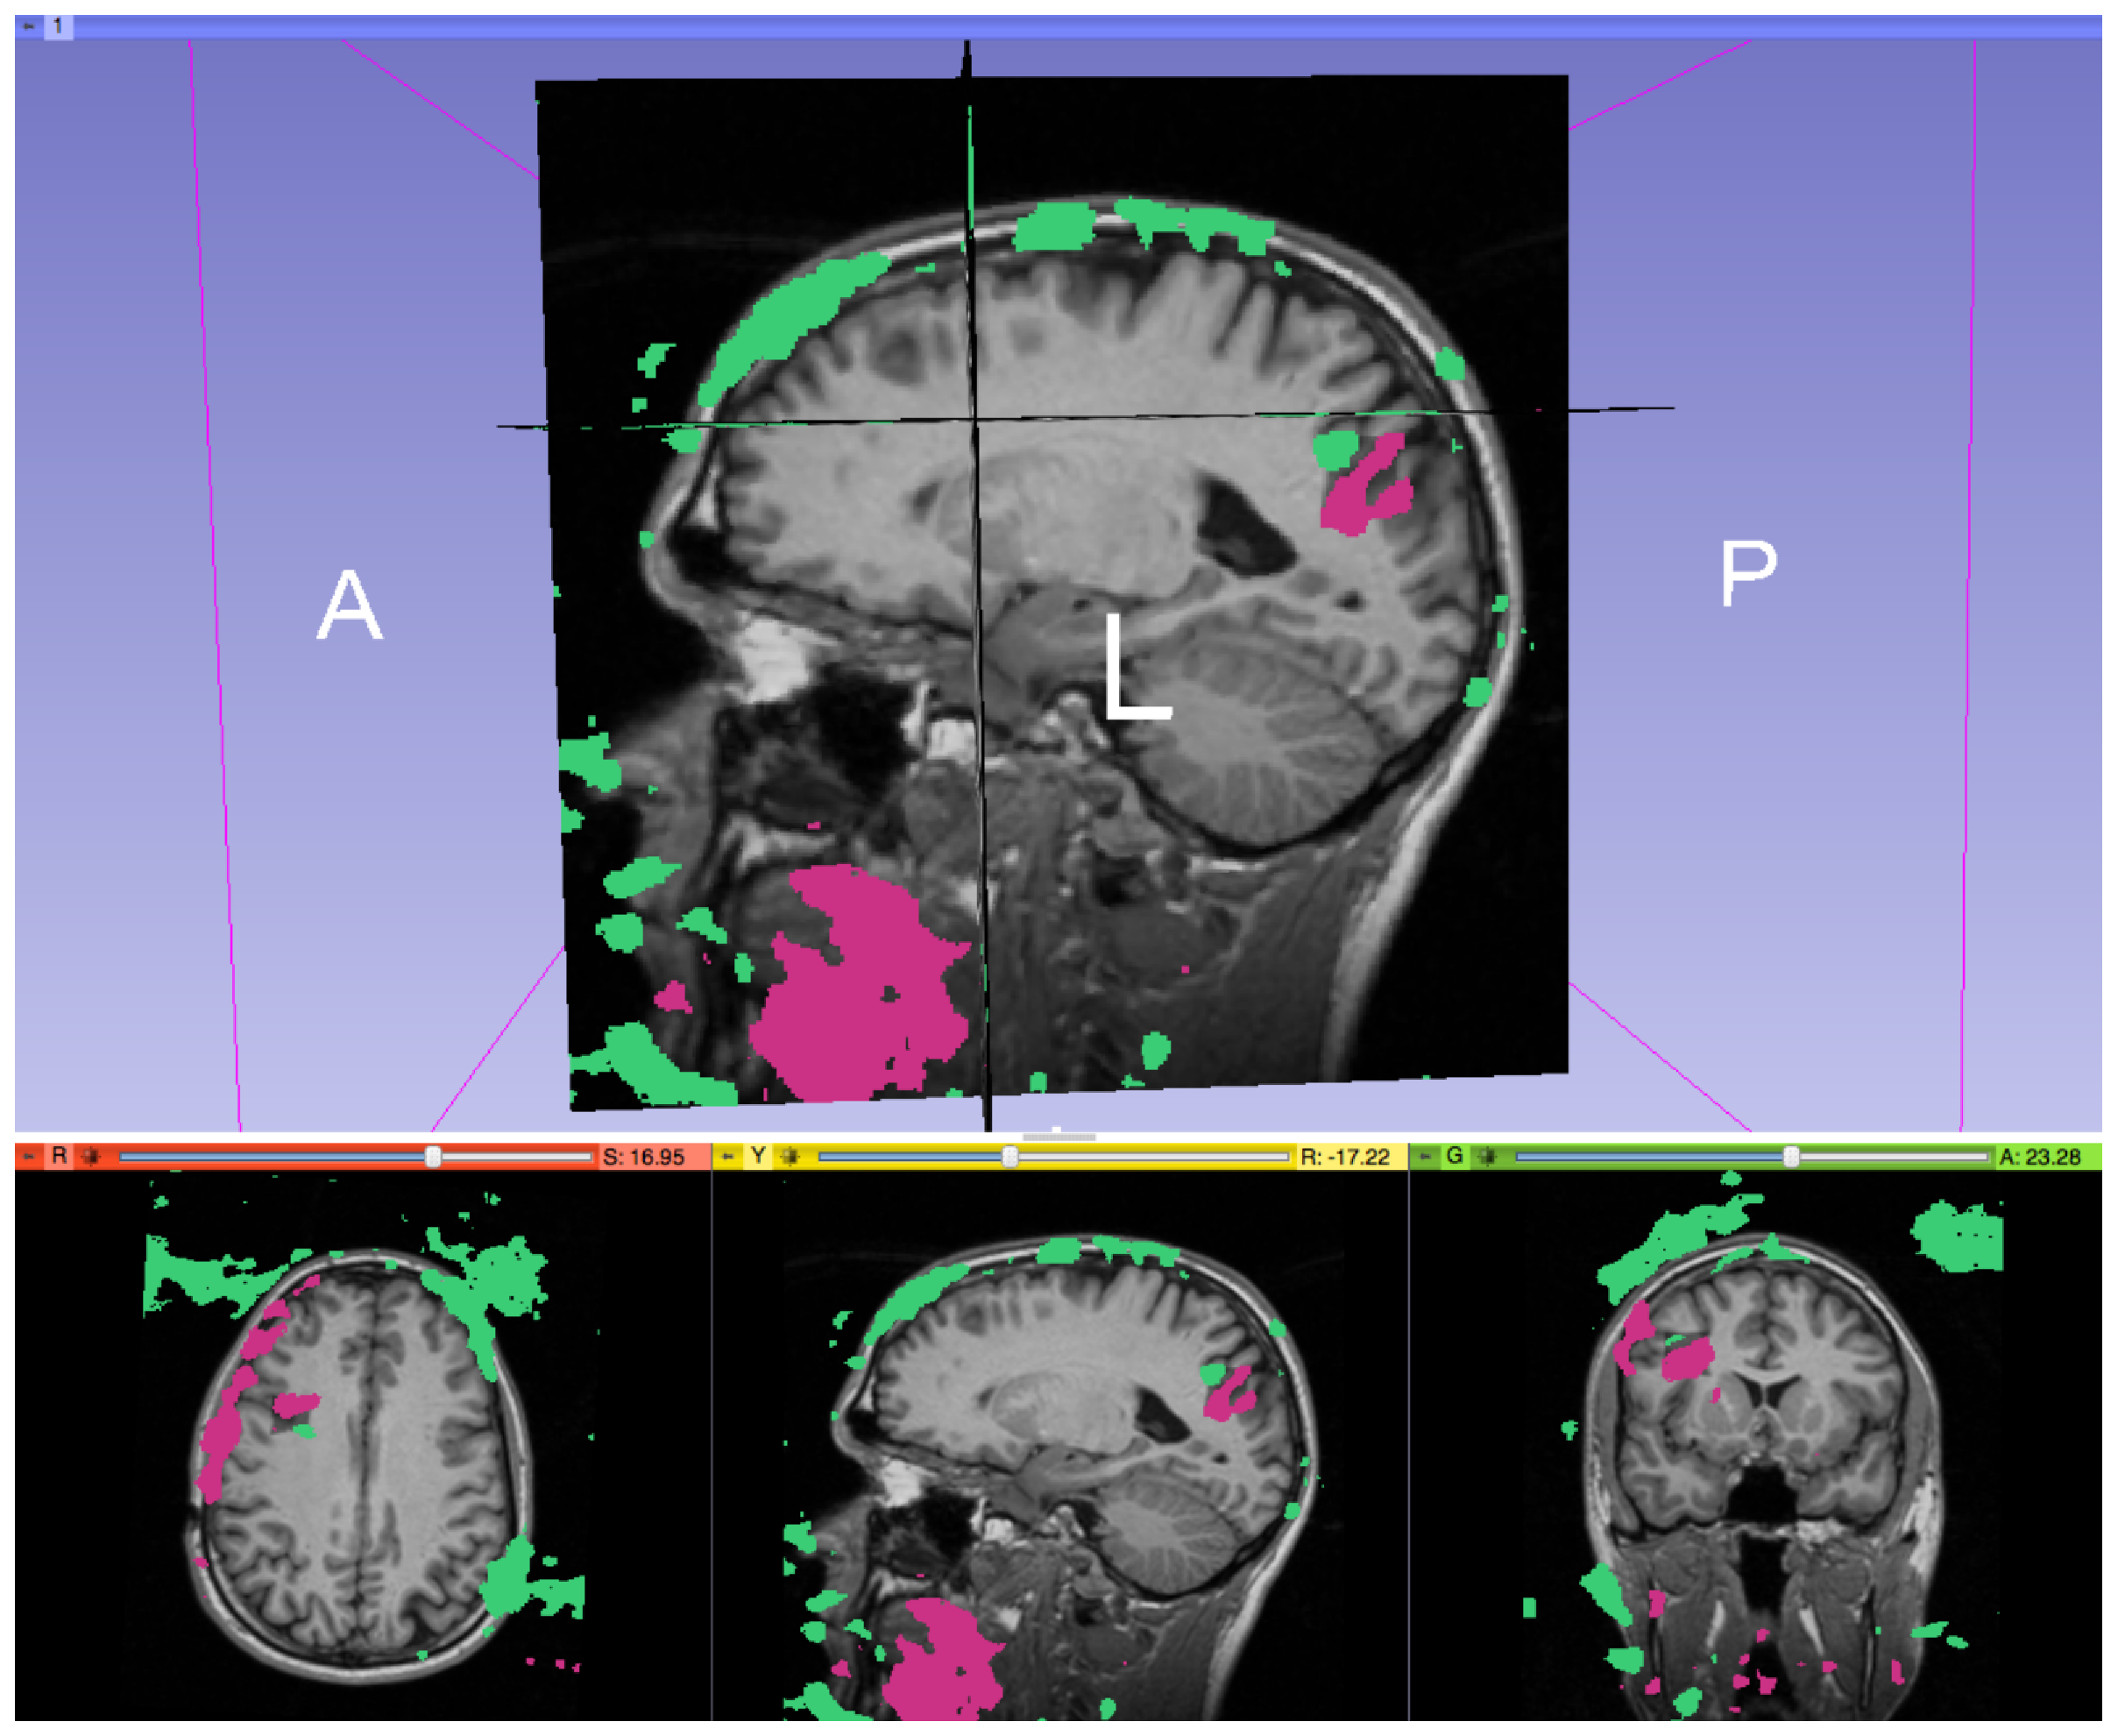
\includegraphics[scale=0.2]{/experiment_bigger/tensor80-65_bigger1.eps}
  \caption{Artificial Large: Tensor-base method}
  \label{tensor_large1}
\end{figure}

Another angle of the result:

\begin{figure}[H]
  \centering
  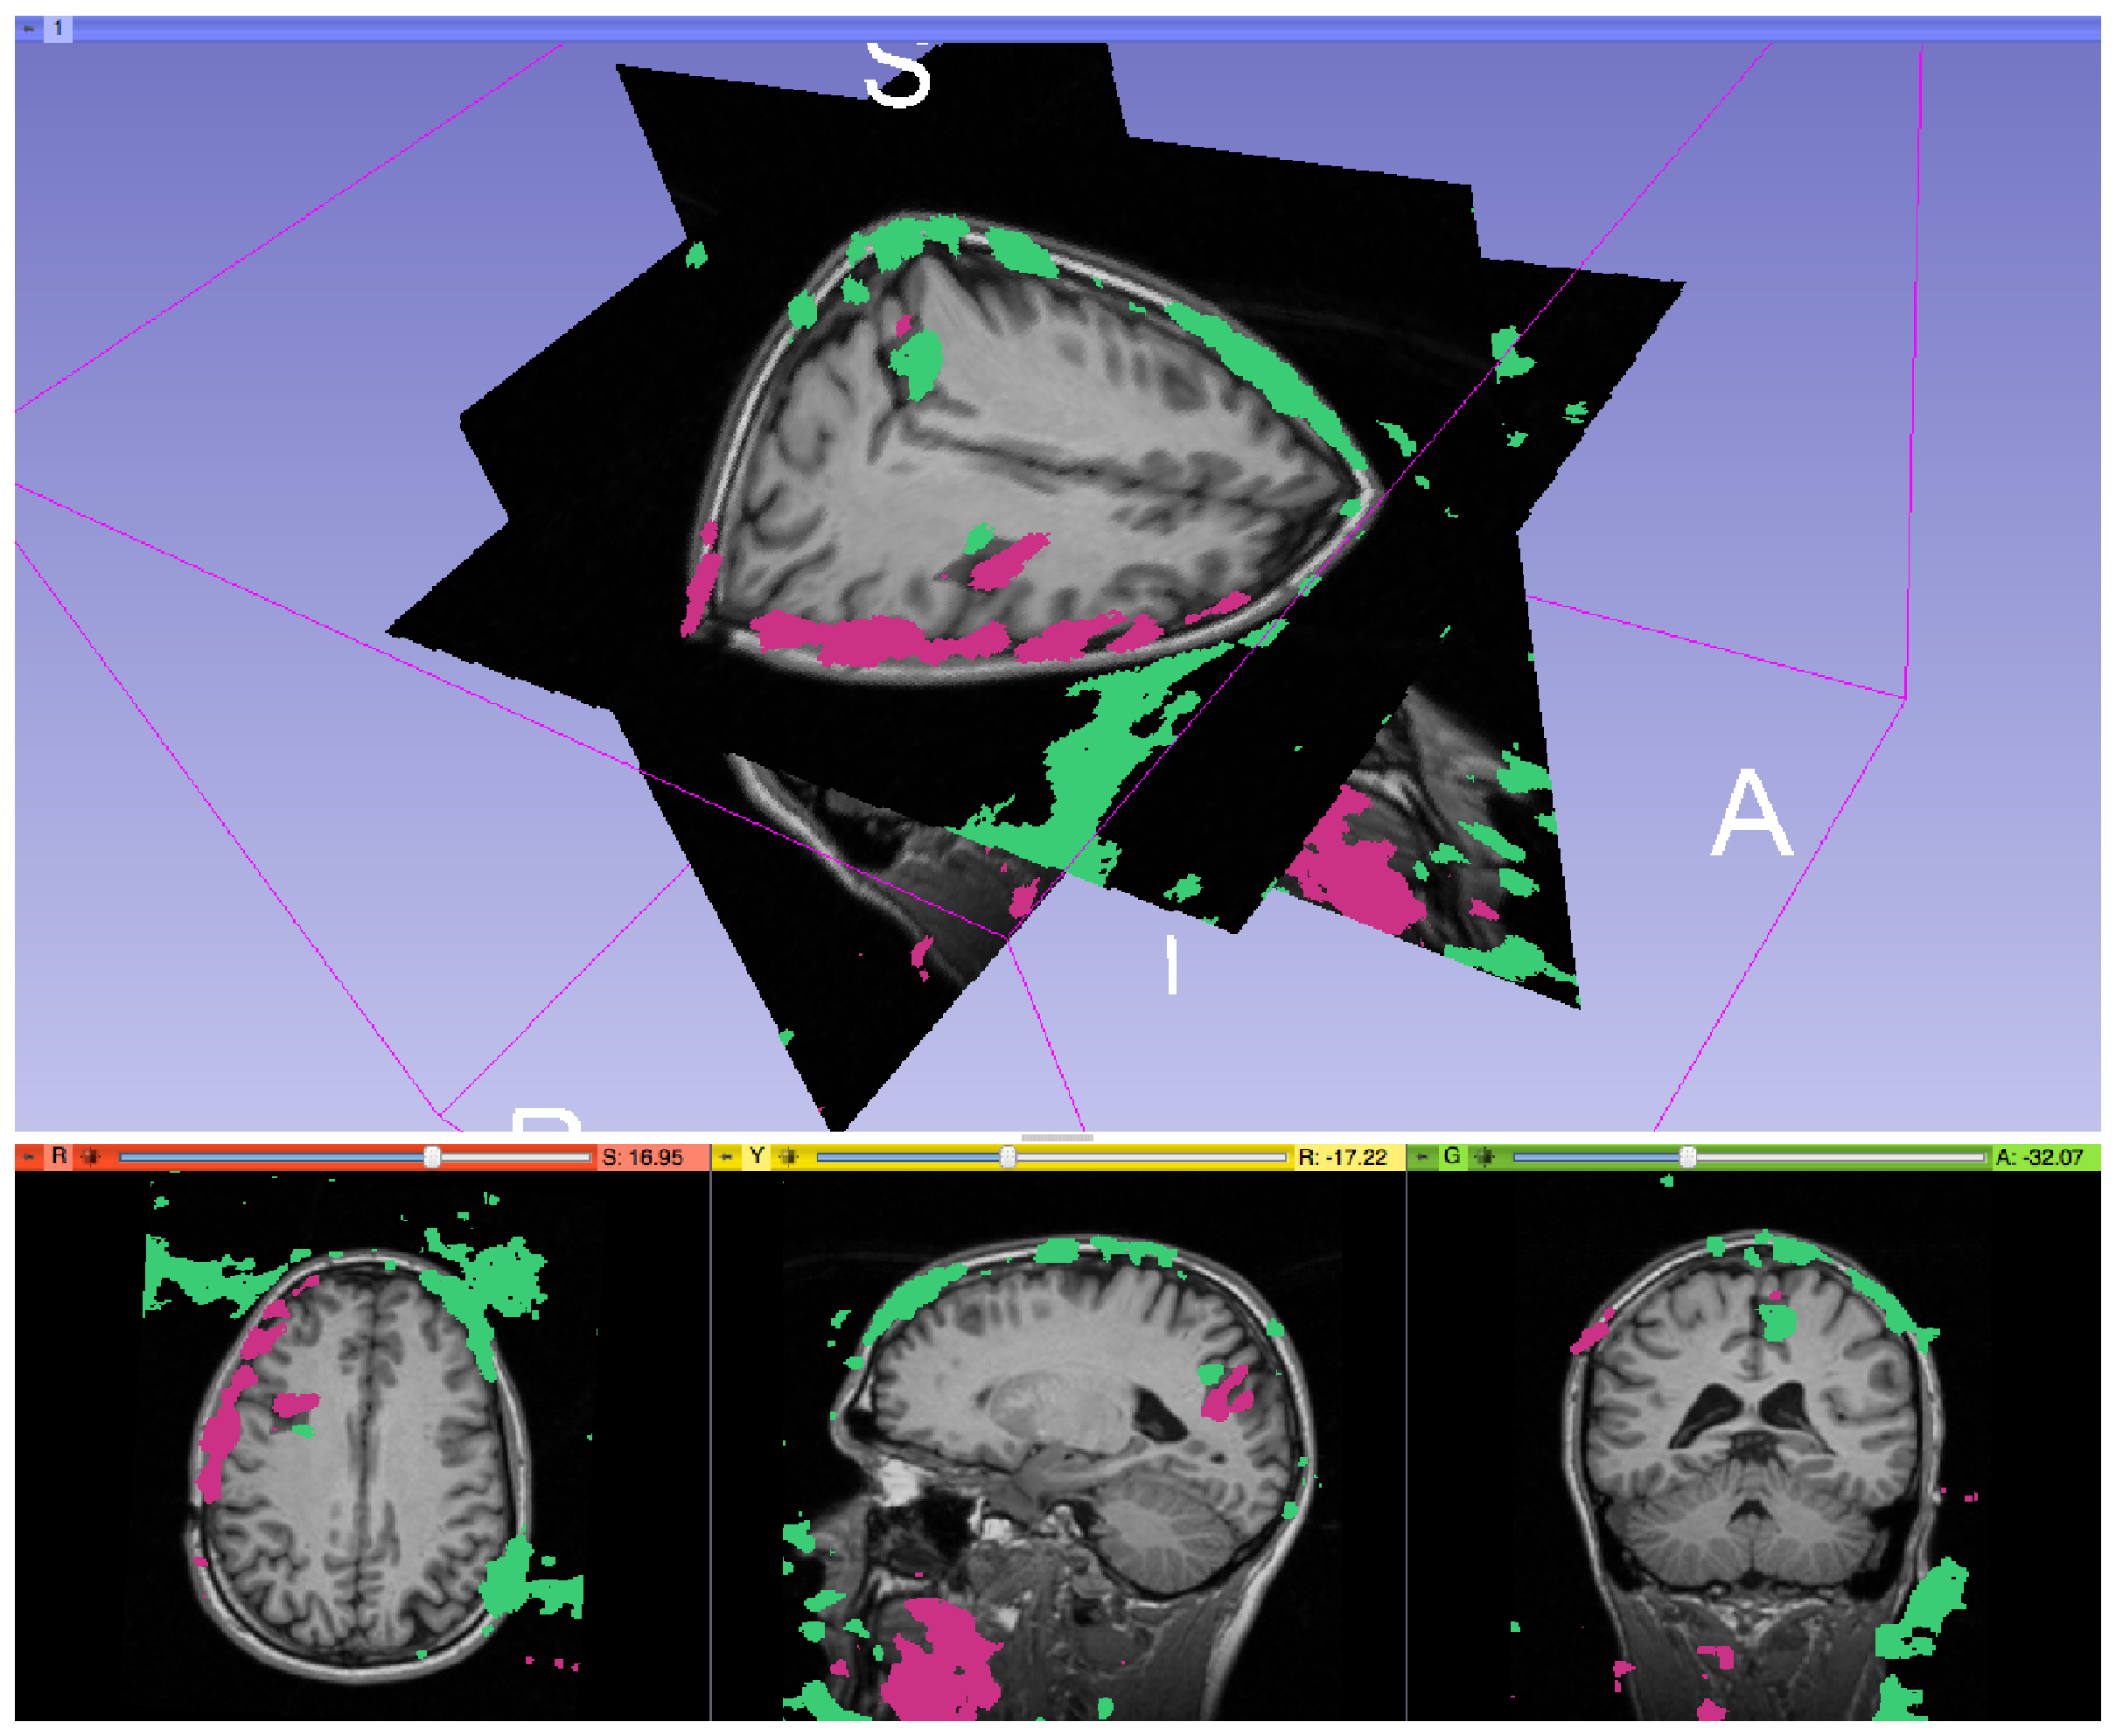
\includegraphics[scale=0.2]{/experiment_bigger/tensor80_65_bigger2.eps}
  \caption{Artificial Large: Tensor-base method}
  \label{tensor_large2}
\end{figure}


\subsection{Size: Medium}
Cubes of medium size where deleted from the follow-up volume to
represent areas of volume loss. The following volume was obtained:

\begin{figure}[H]
  \centering
  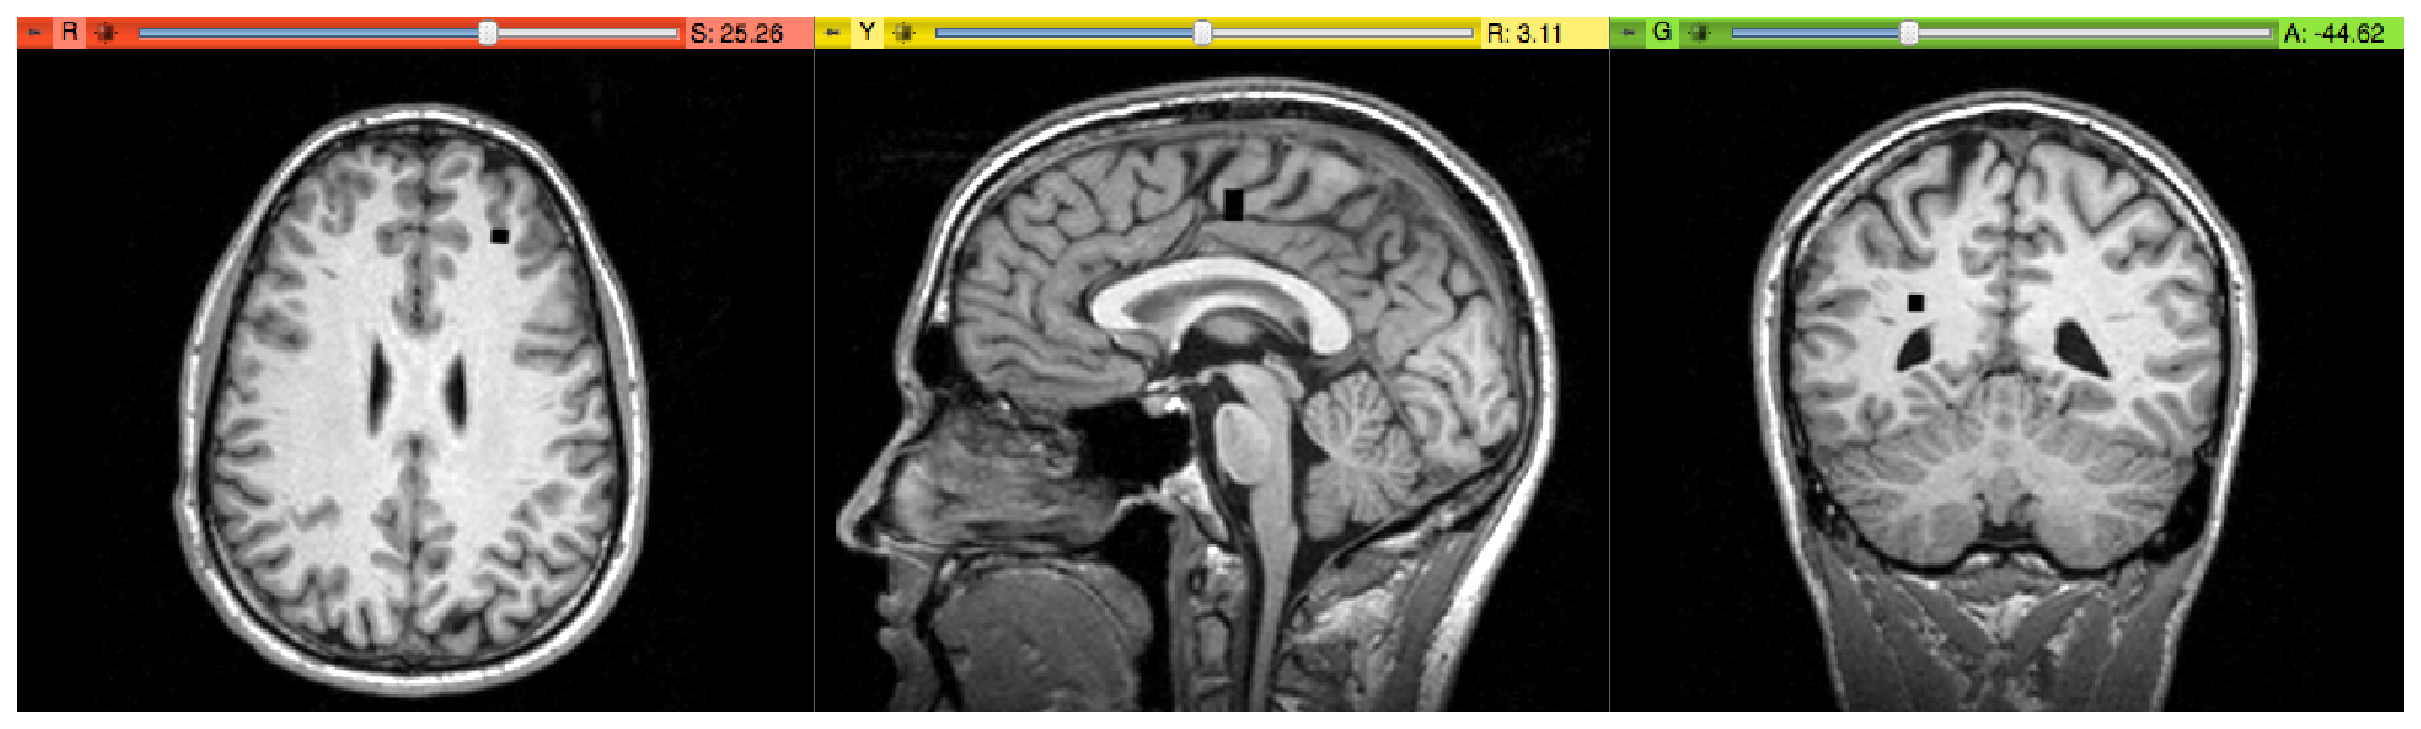
\includegraphics[scale=0.3]{/experiment_medium/medB_subtracted.eps}
  \caption{Medium Differences: Modified Follow-up volume}
  \label{largeB}
\end{figure}

\subsubsection{Voxel-based Method}
The result obtained with this method and medium differences is as good
as with larger differences. All the deleted volume cubes are found and
easy to see in the result.

\begin{figure}[H]
  \centering
  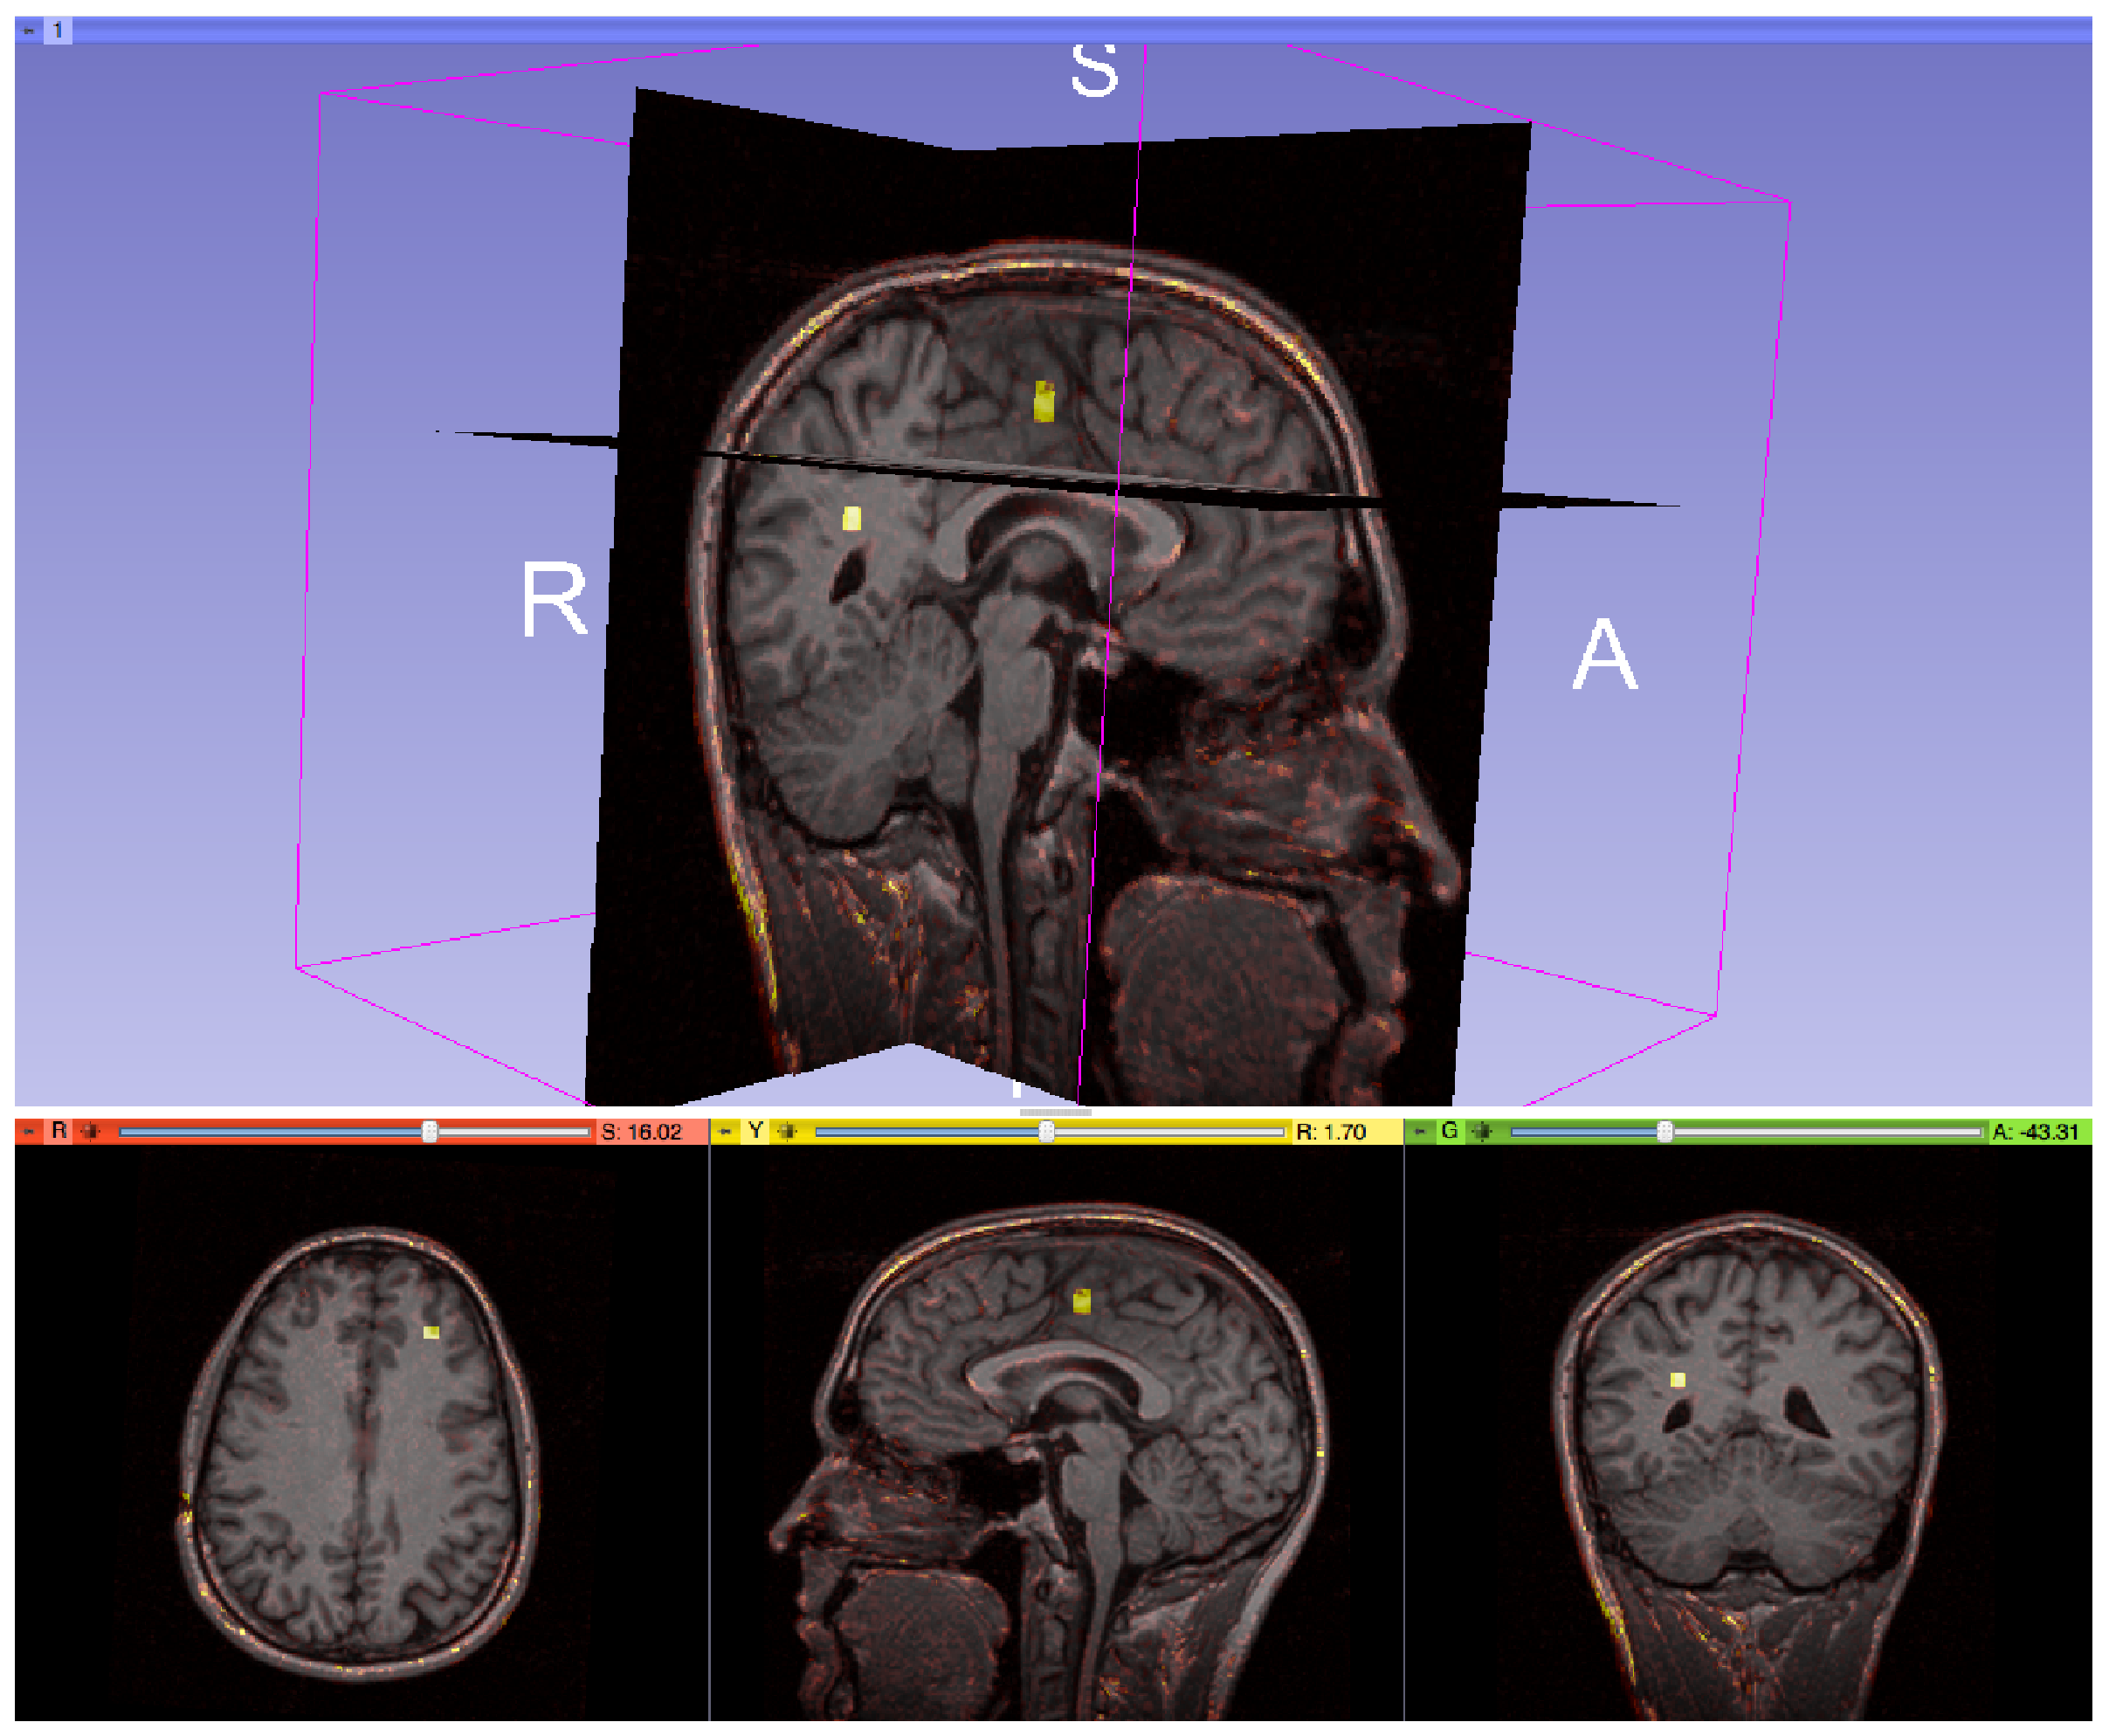
\includegraphics[scale=0.2]{/experiment_medium/med_voxel1.eps}
  \caption{Artificial Medium: Voxel-base method}
  \label{voxel_med1}
\end{figure}

Another angle of the result:

\begin{figure}[H]
  \centering
  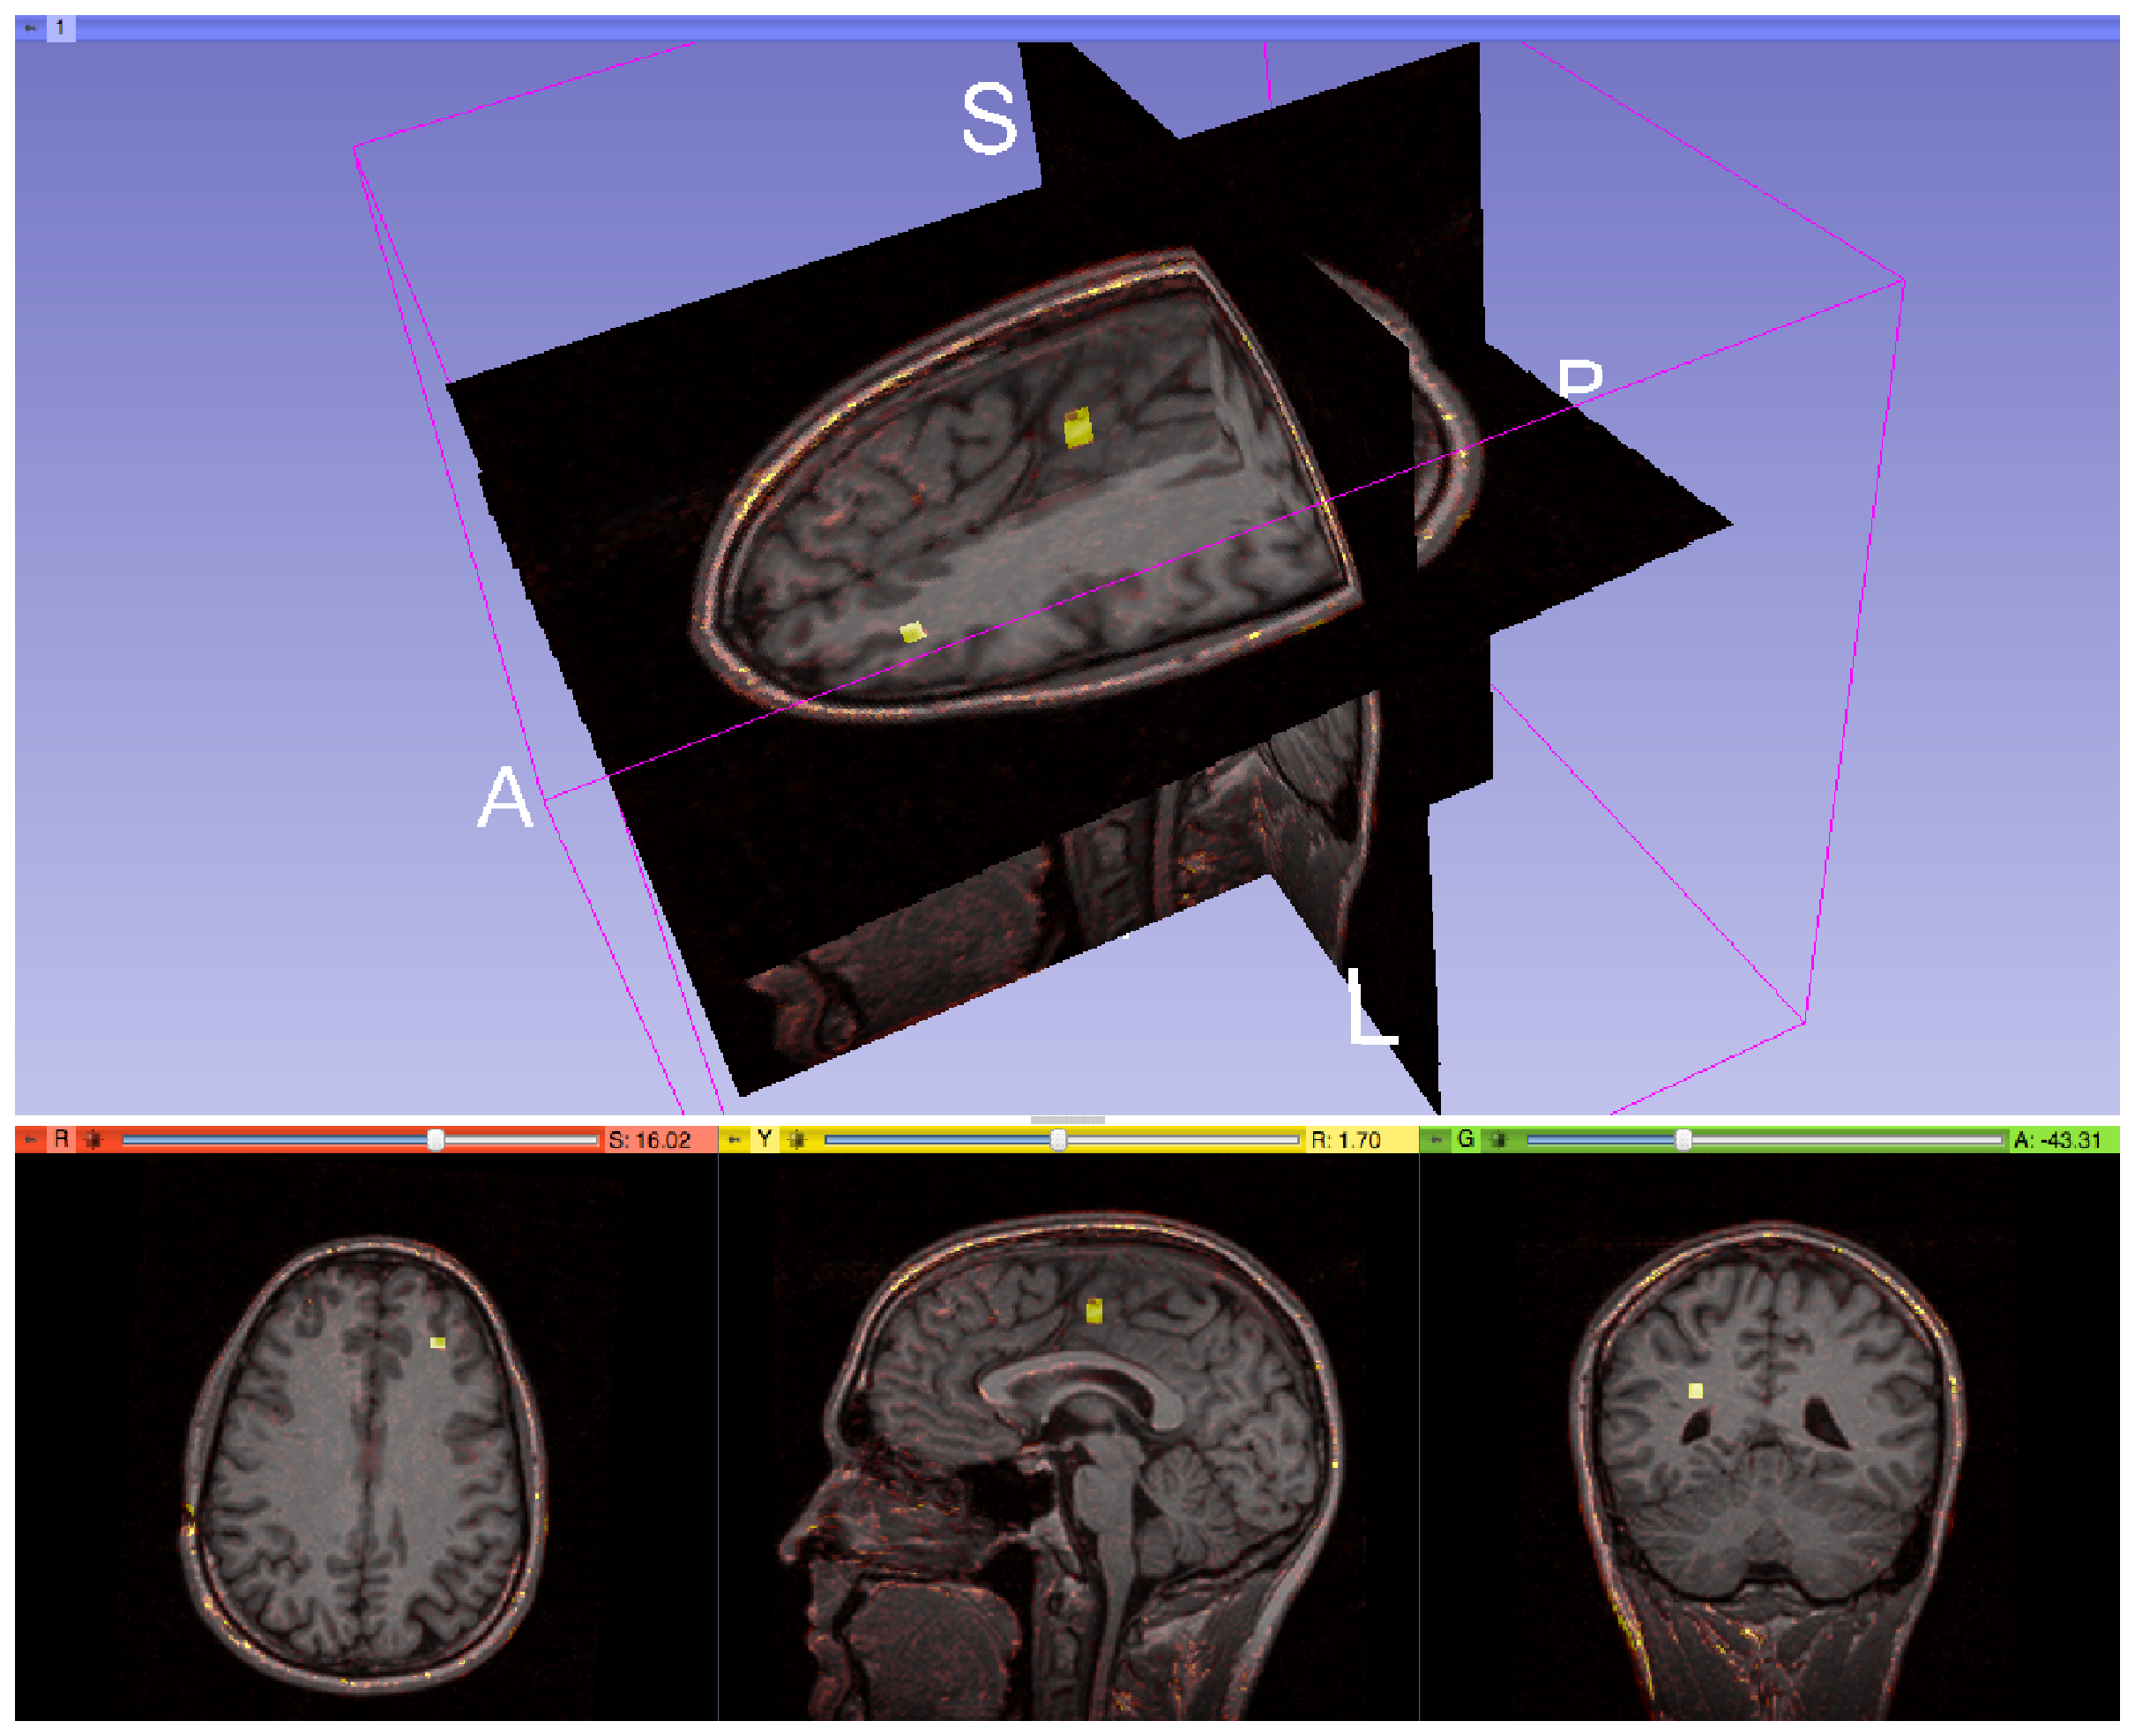
\includegraphics[scale=0.2]{/experiment_medium/med_voxel2.eps}
  \caption{Artificial Medium: Voxel-base method}
  \label{voxel_med2}
\end{figure}

\subsubsection{Tensor-based Method}
The result is a bit worse than for bigger differences. The volume
losses are still found by the application, but their borders are not
defined and the method also founds other zones with differences that
are hard to differenciate from the added ones.

The parameters used to obtain this result are:
\begin{description}
\item \textit{Deformation field smoothing sigma:} 2.5
\item \textit{Shrinkage percentage:} 80
\item \textit{Growth percentage:} 76
\end{description}

\begin{figure}[H]
  \centering
  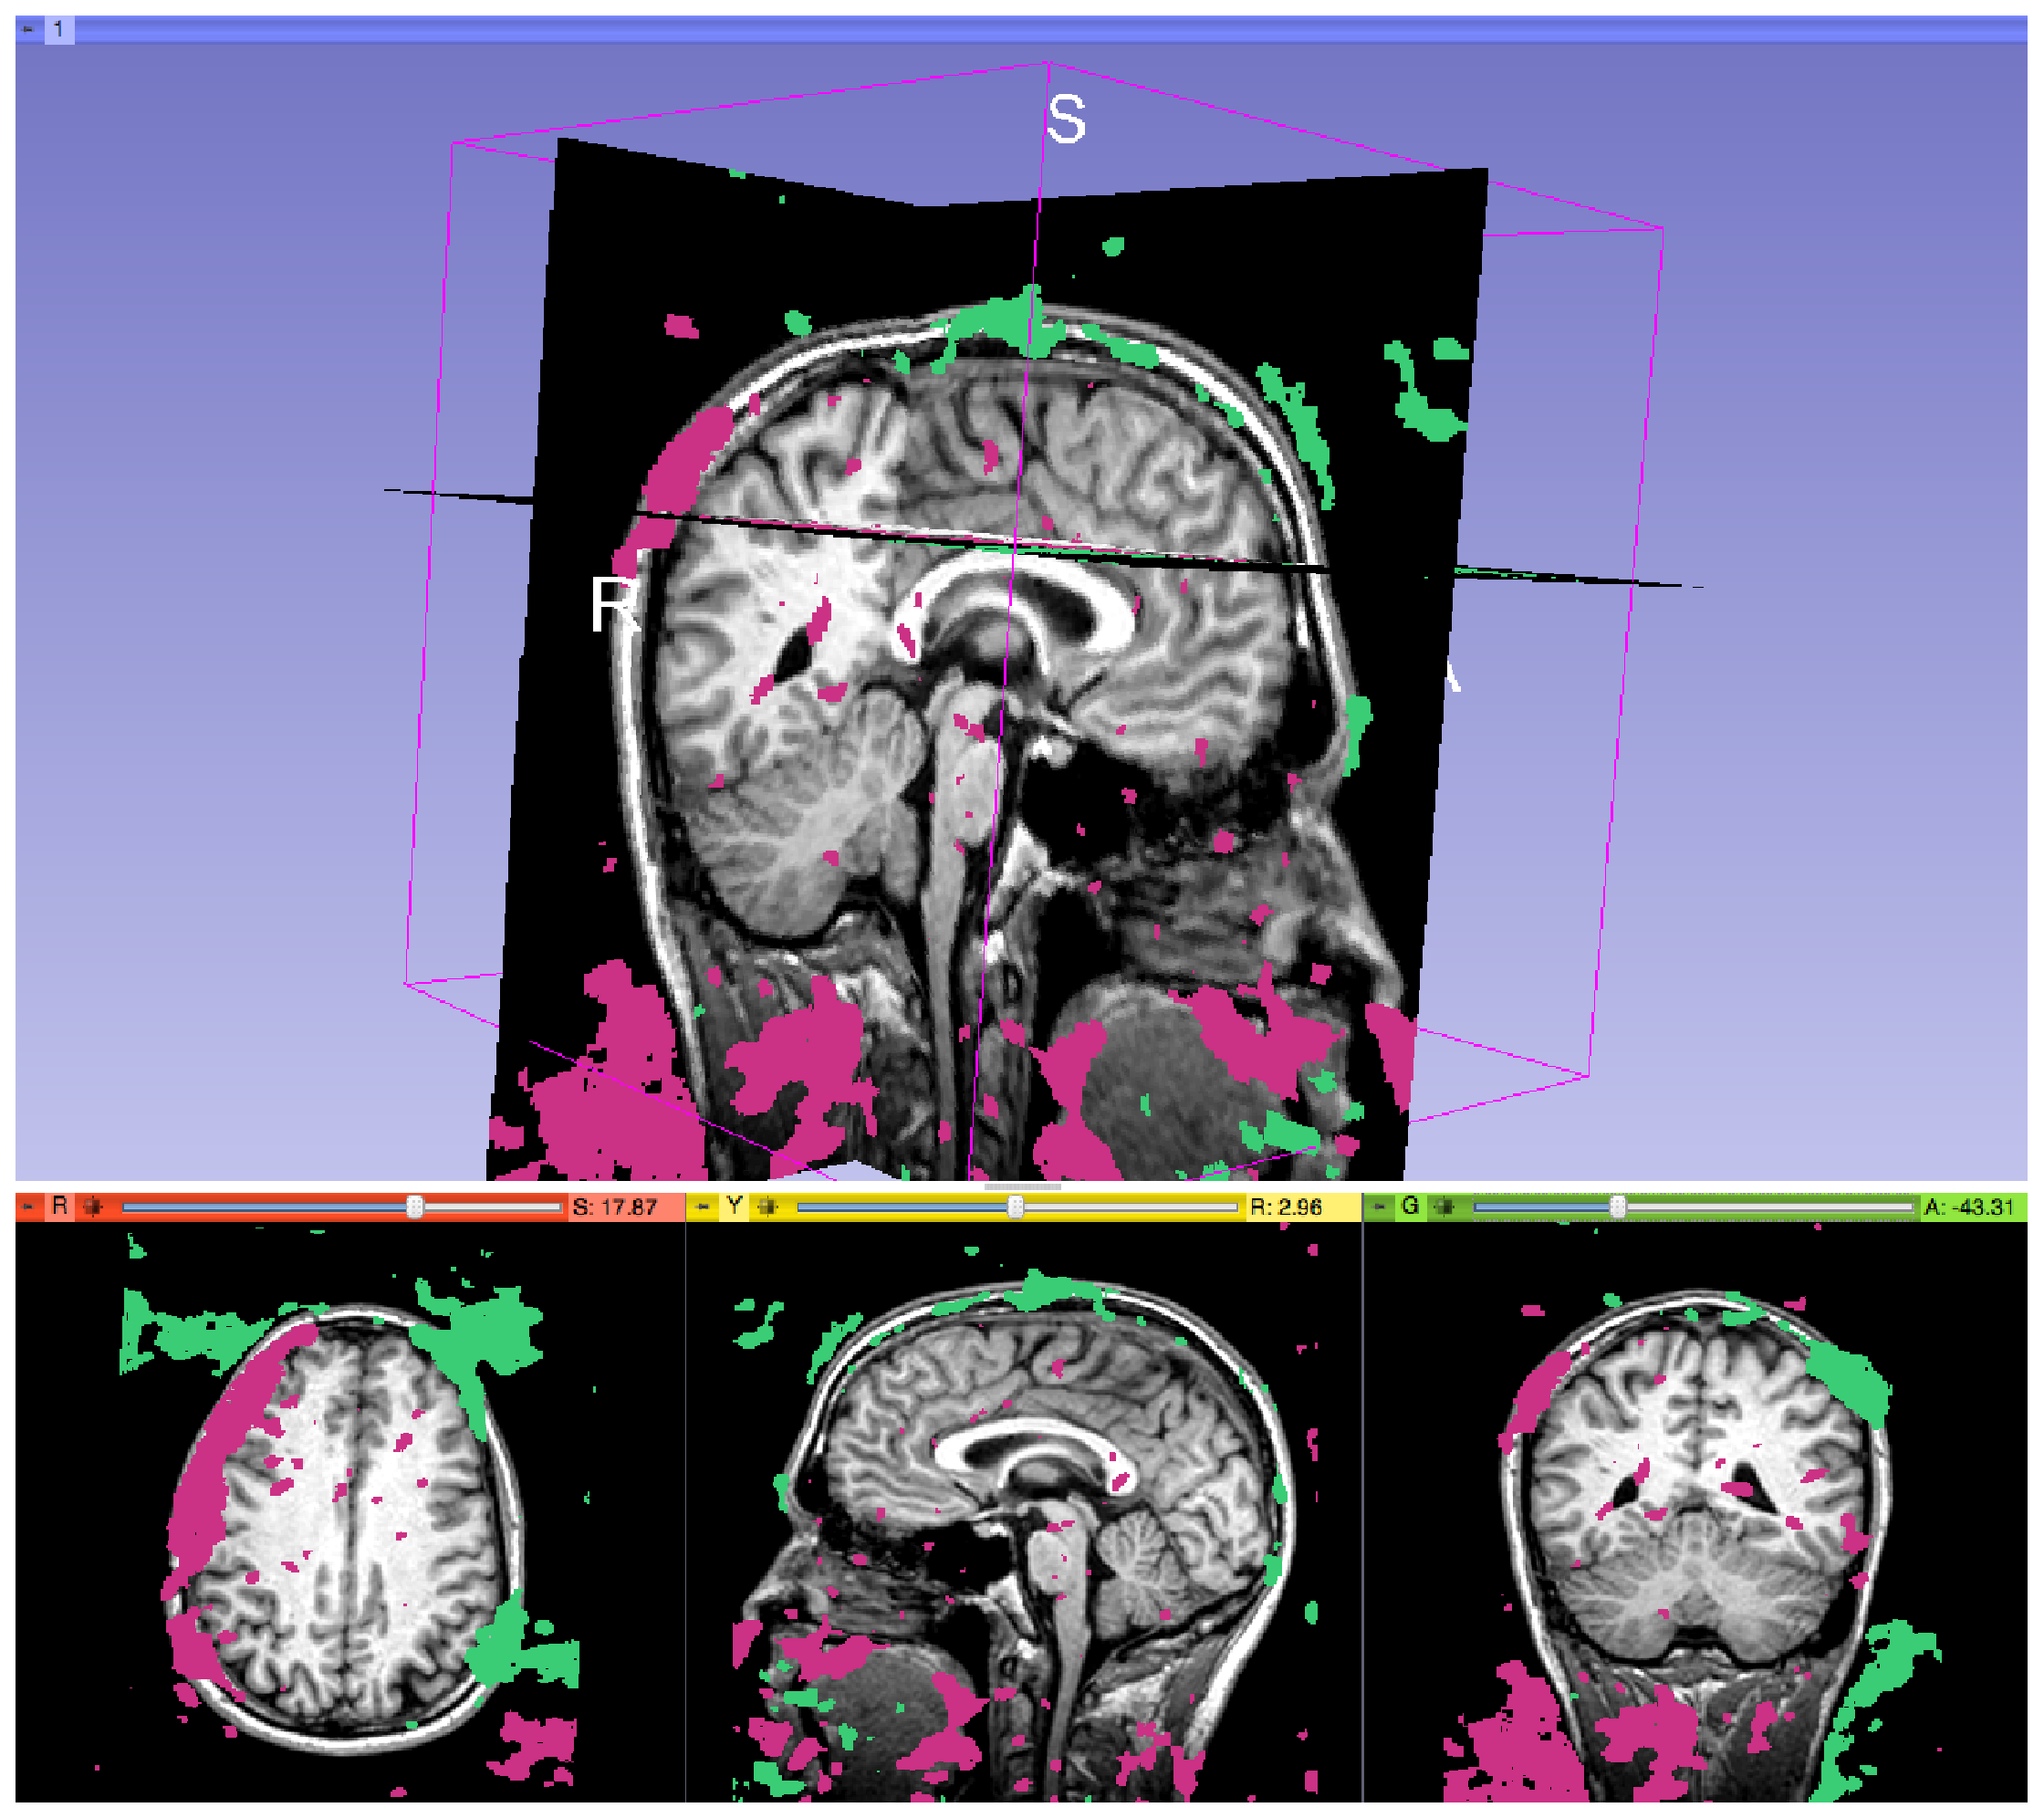
\includegraphics[scale=0.2]{/experiment_medium/tensor80-76_med1.eps}
  \caption{Artificial Medium: Tensor-base method}
  \label{tensor_med1}
\end{figure}

Another angle of the result:

\begin{figure}[H]
  \centering
  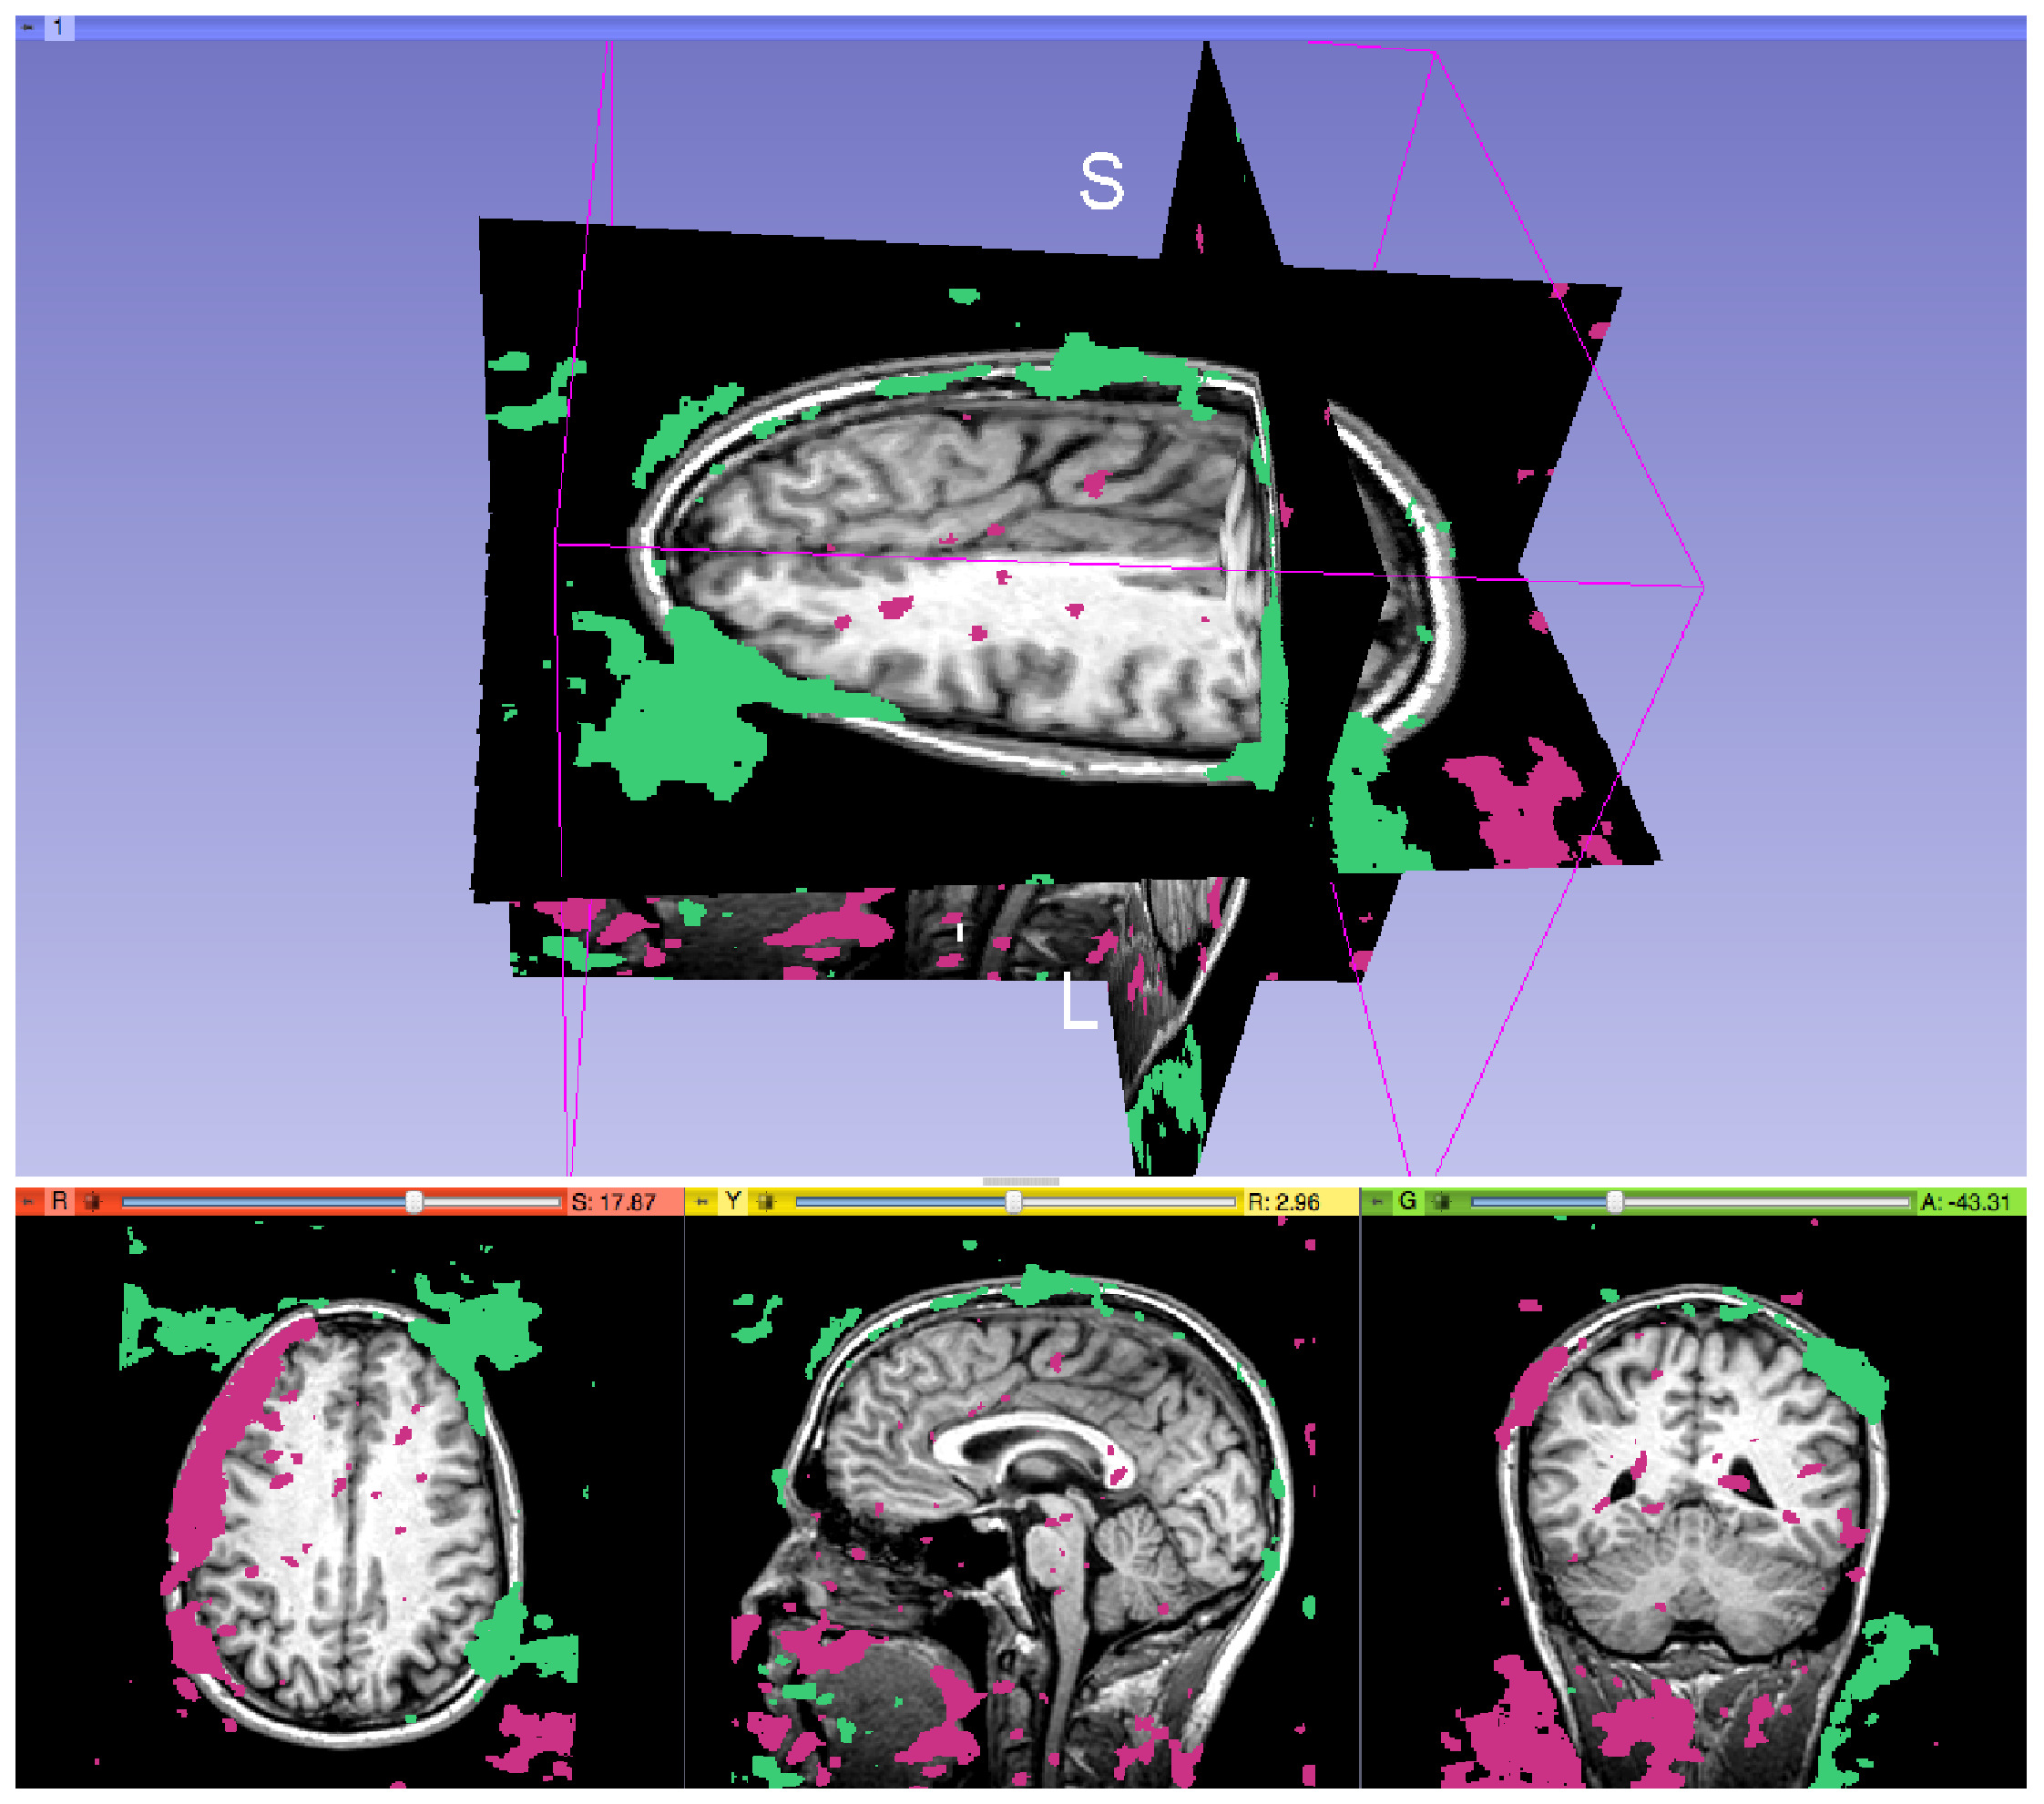
\includegraphics[scale=0.2]{/experiment_medium/tensor80-76_med2.eps}
  \caption{Artificial Medium: Tensor-base method}
  \label{tensor_med2}
\end{figure}

\subsection{Size: Small}
Rectangles of very small size where deleted from the follow-up volume
to represent areas of volume loss. Rectangles were selected instead of
cubes in this case in order to be able to view the result more simply.

The following volume was obtained. In this image, the small rectangles
are marked in red just for the purpose of being more visible in this
report. The original image does not include the red circles:

\begin{figure}[H]
  \centering
  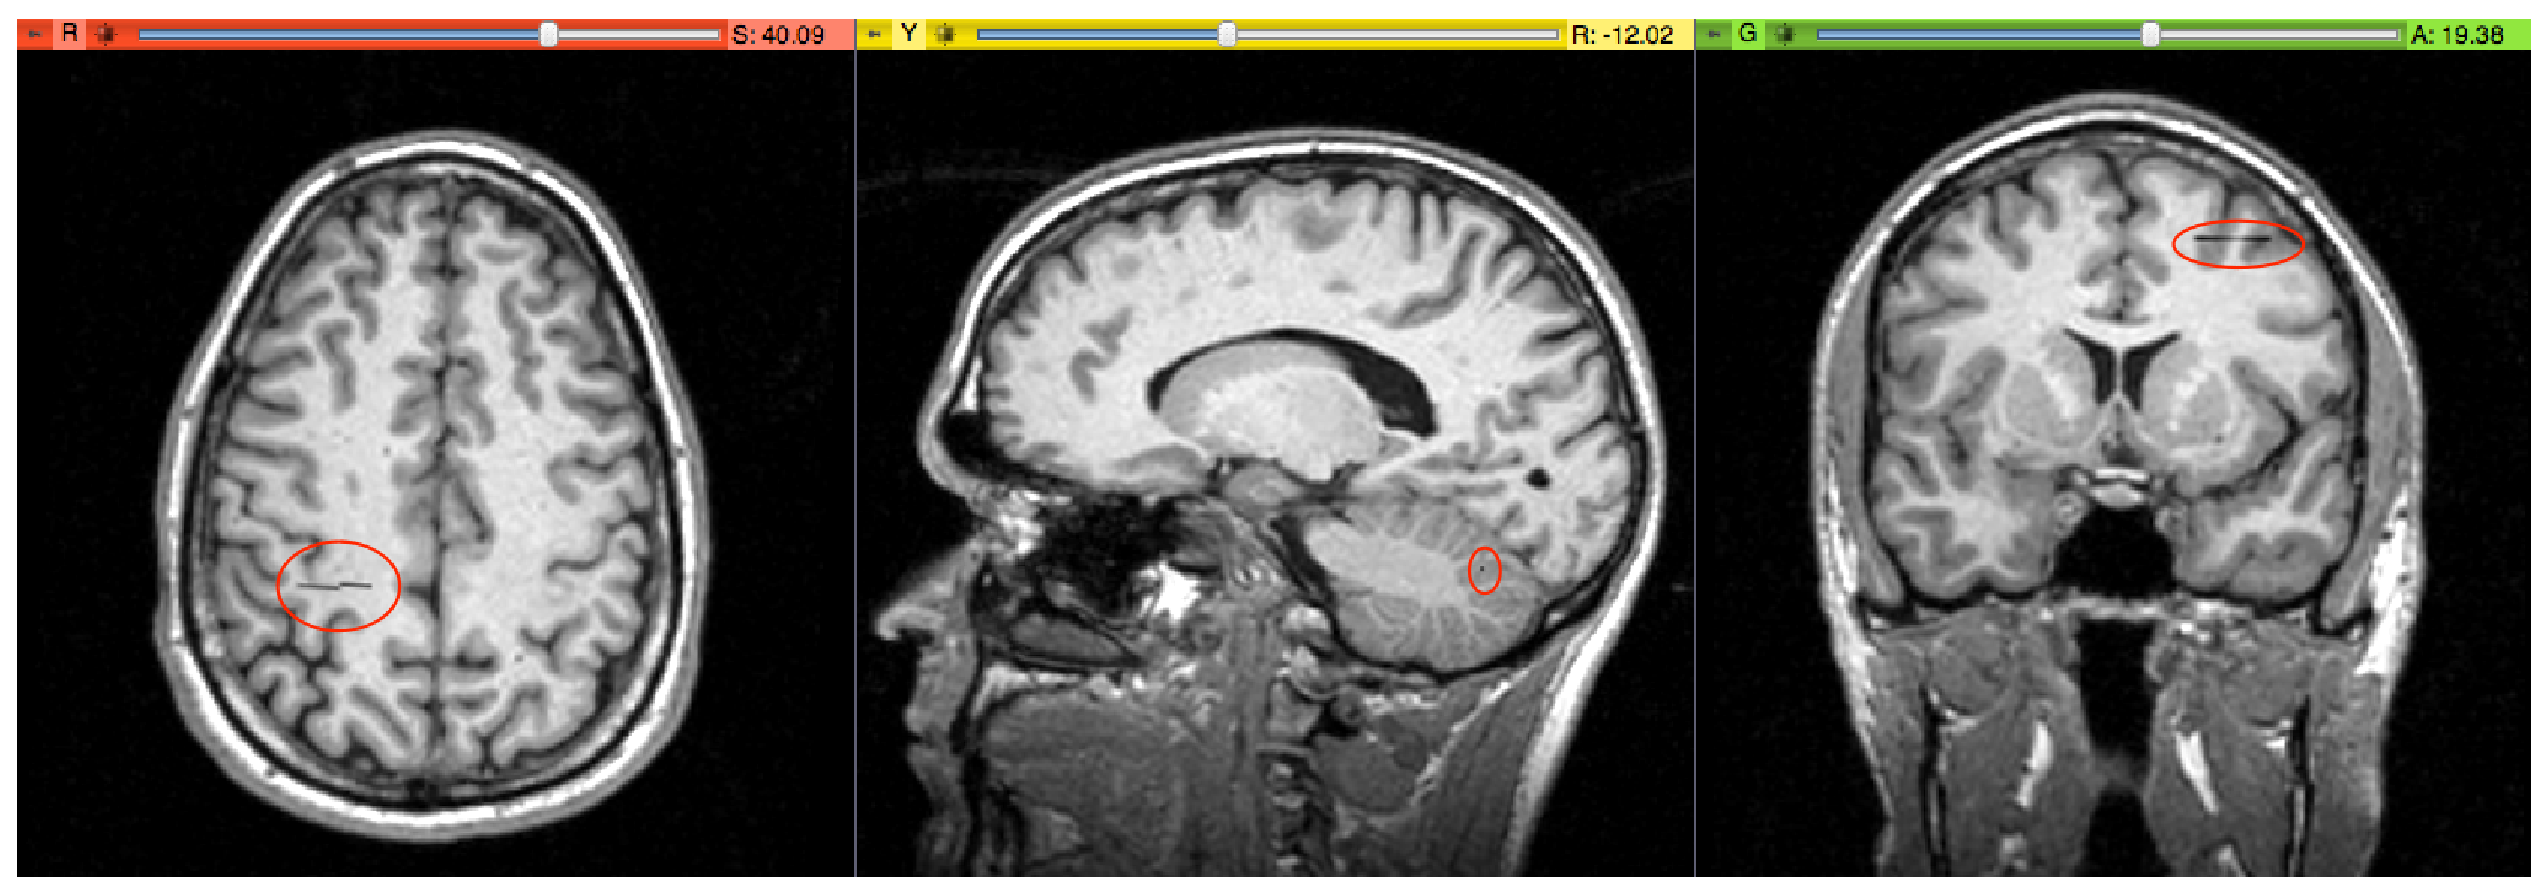
\includegraphics[scale=0.3]{/experiment_small/small_differences.eps}
  \caption{Small Differences: Modified Follow-up volume}
  \label{smallB}
\end{figure}

\subsubsection{Voxel-based Method}
The result obtained with this method and small differences is also
very good. All the deleted volume rectagles are found in the result,
although in this case the differences are so small that could be hard
to see, even when they are highlighted in the resulting volume.

\begin{figure}[H]
  \centering
  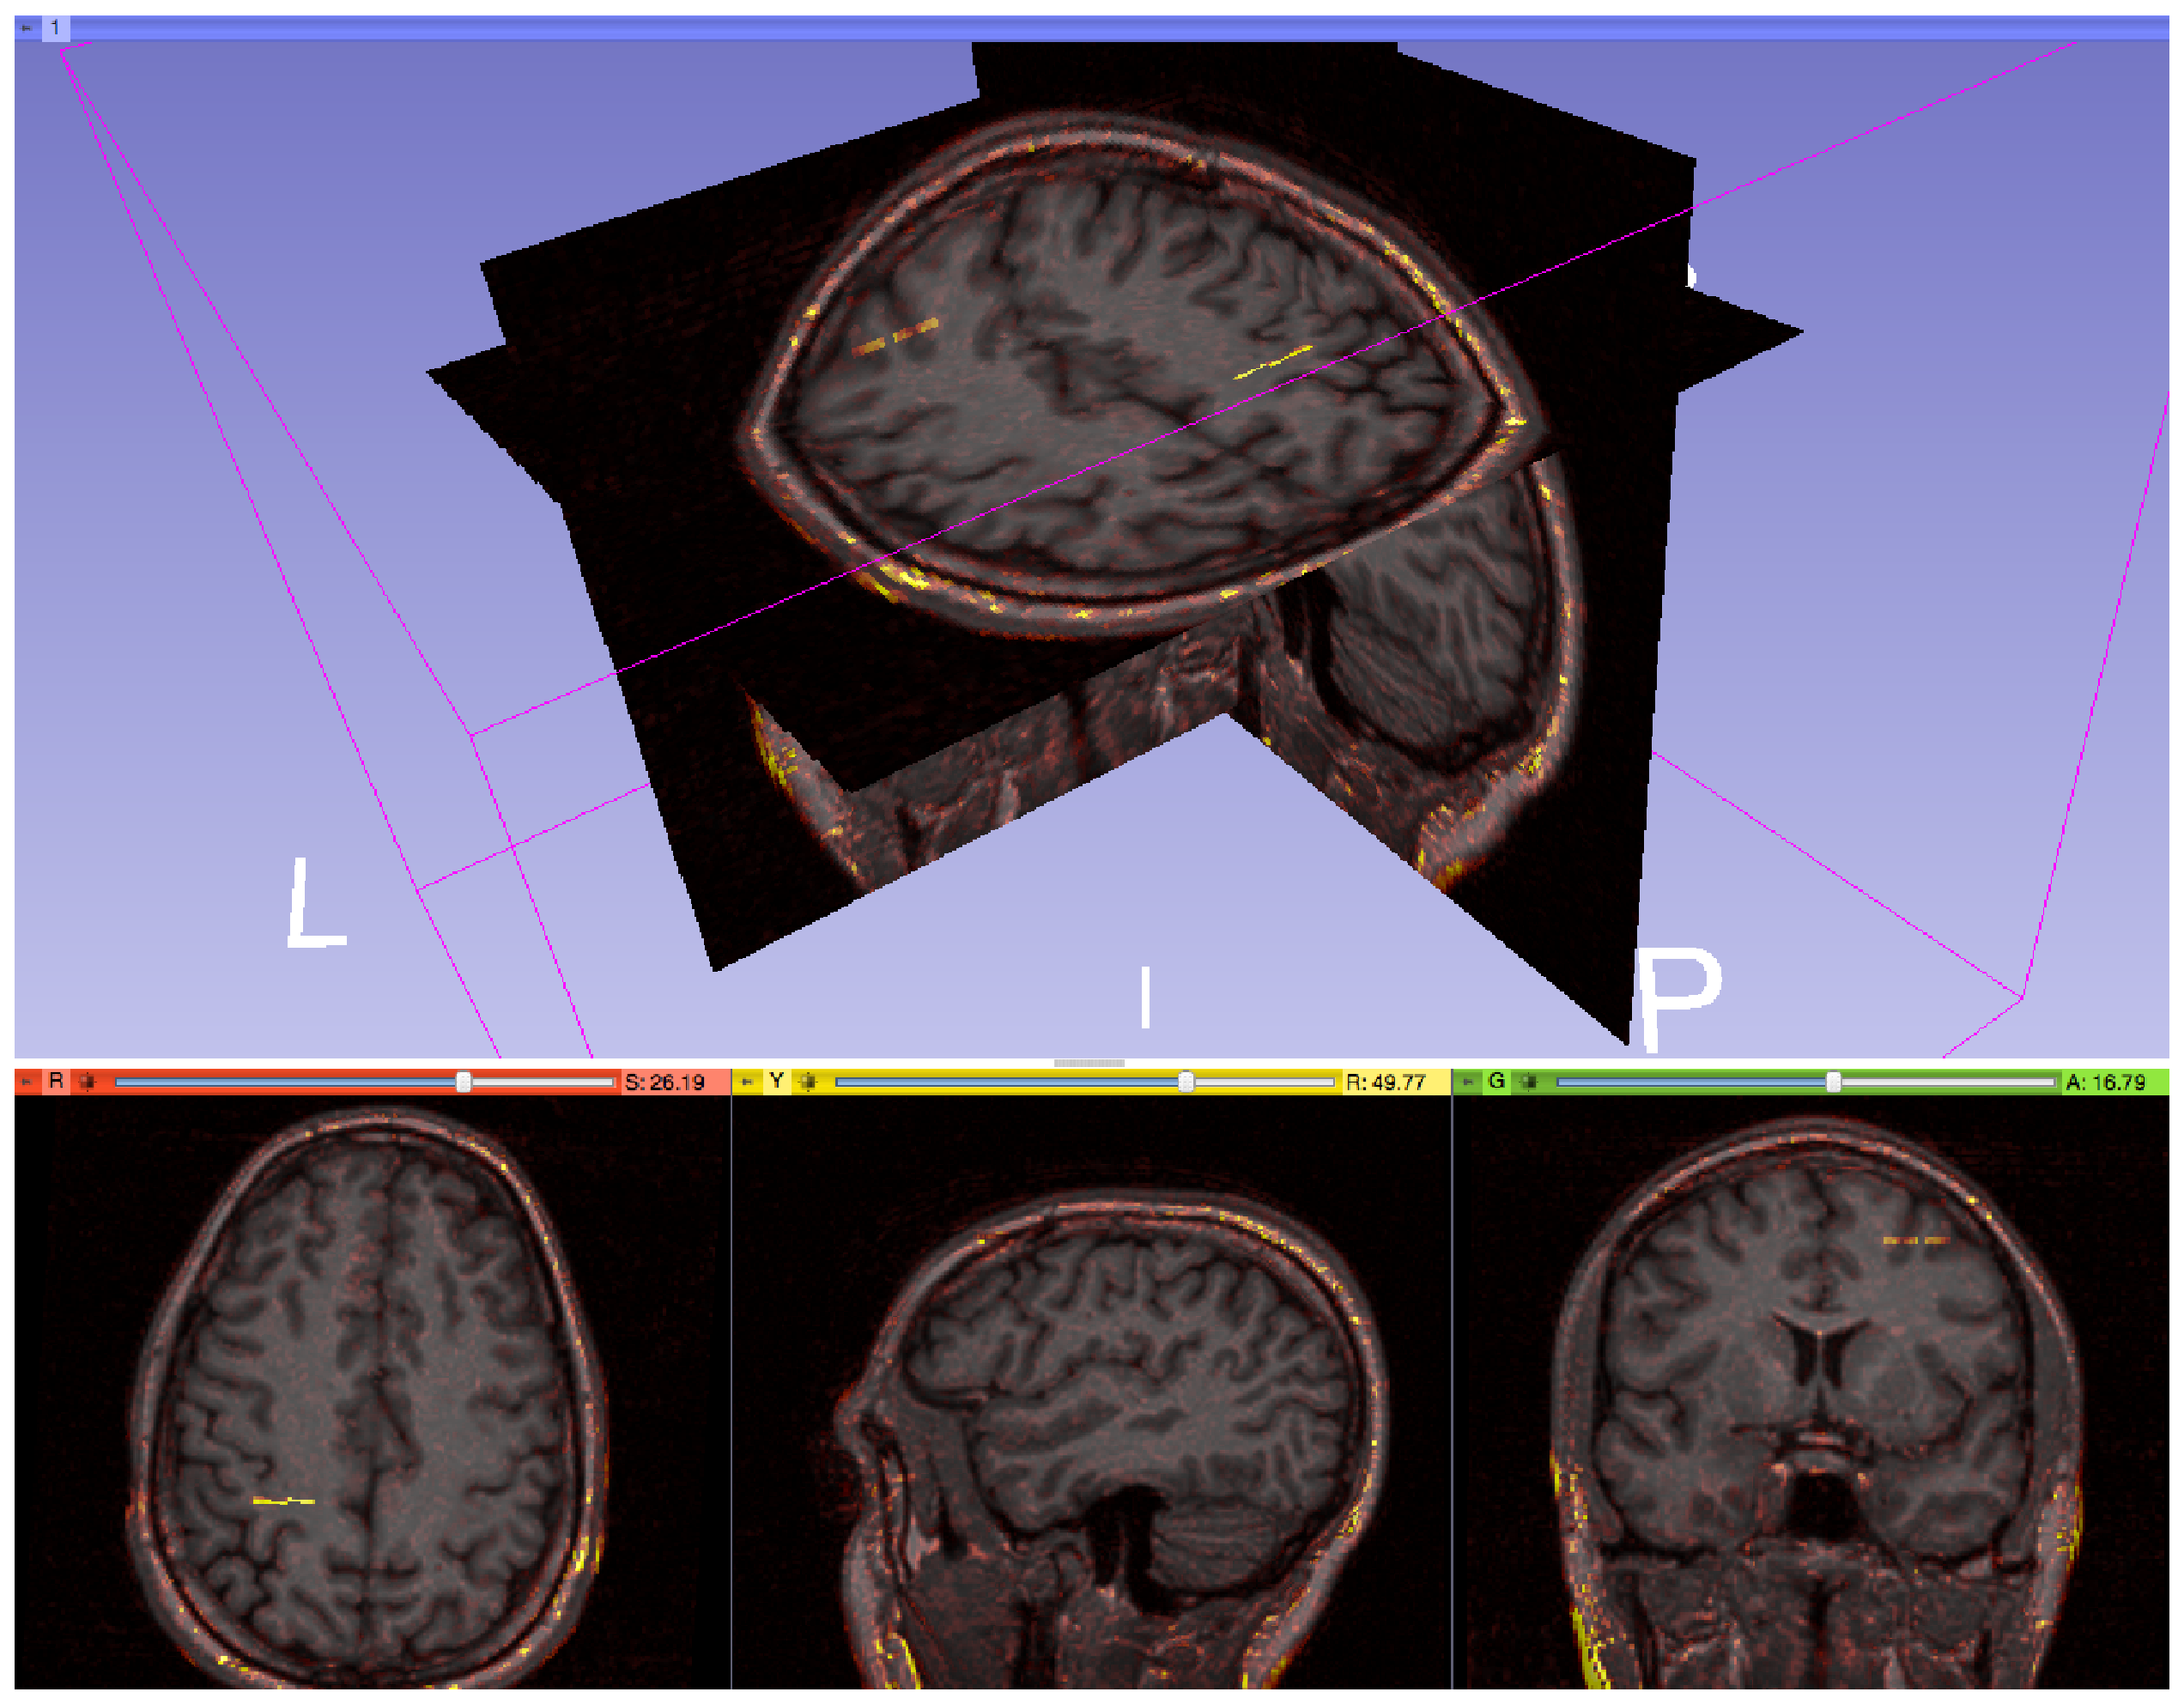
\includegraphics[scale=0.2]{/experiment_small/small_voxel1.eps}
  \caption{Artificial Small: Voxel-base method}
  \label{voxel_small1}
\end{figure}

Another angle of the result:

\begin{figure}[H]
  \centering
  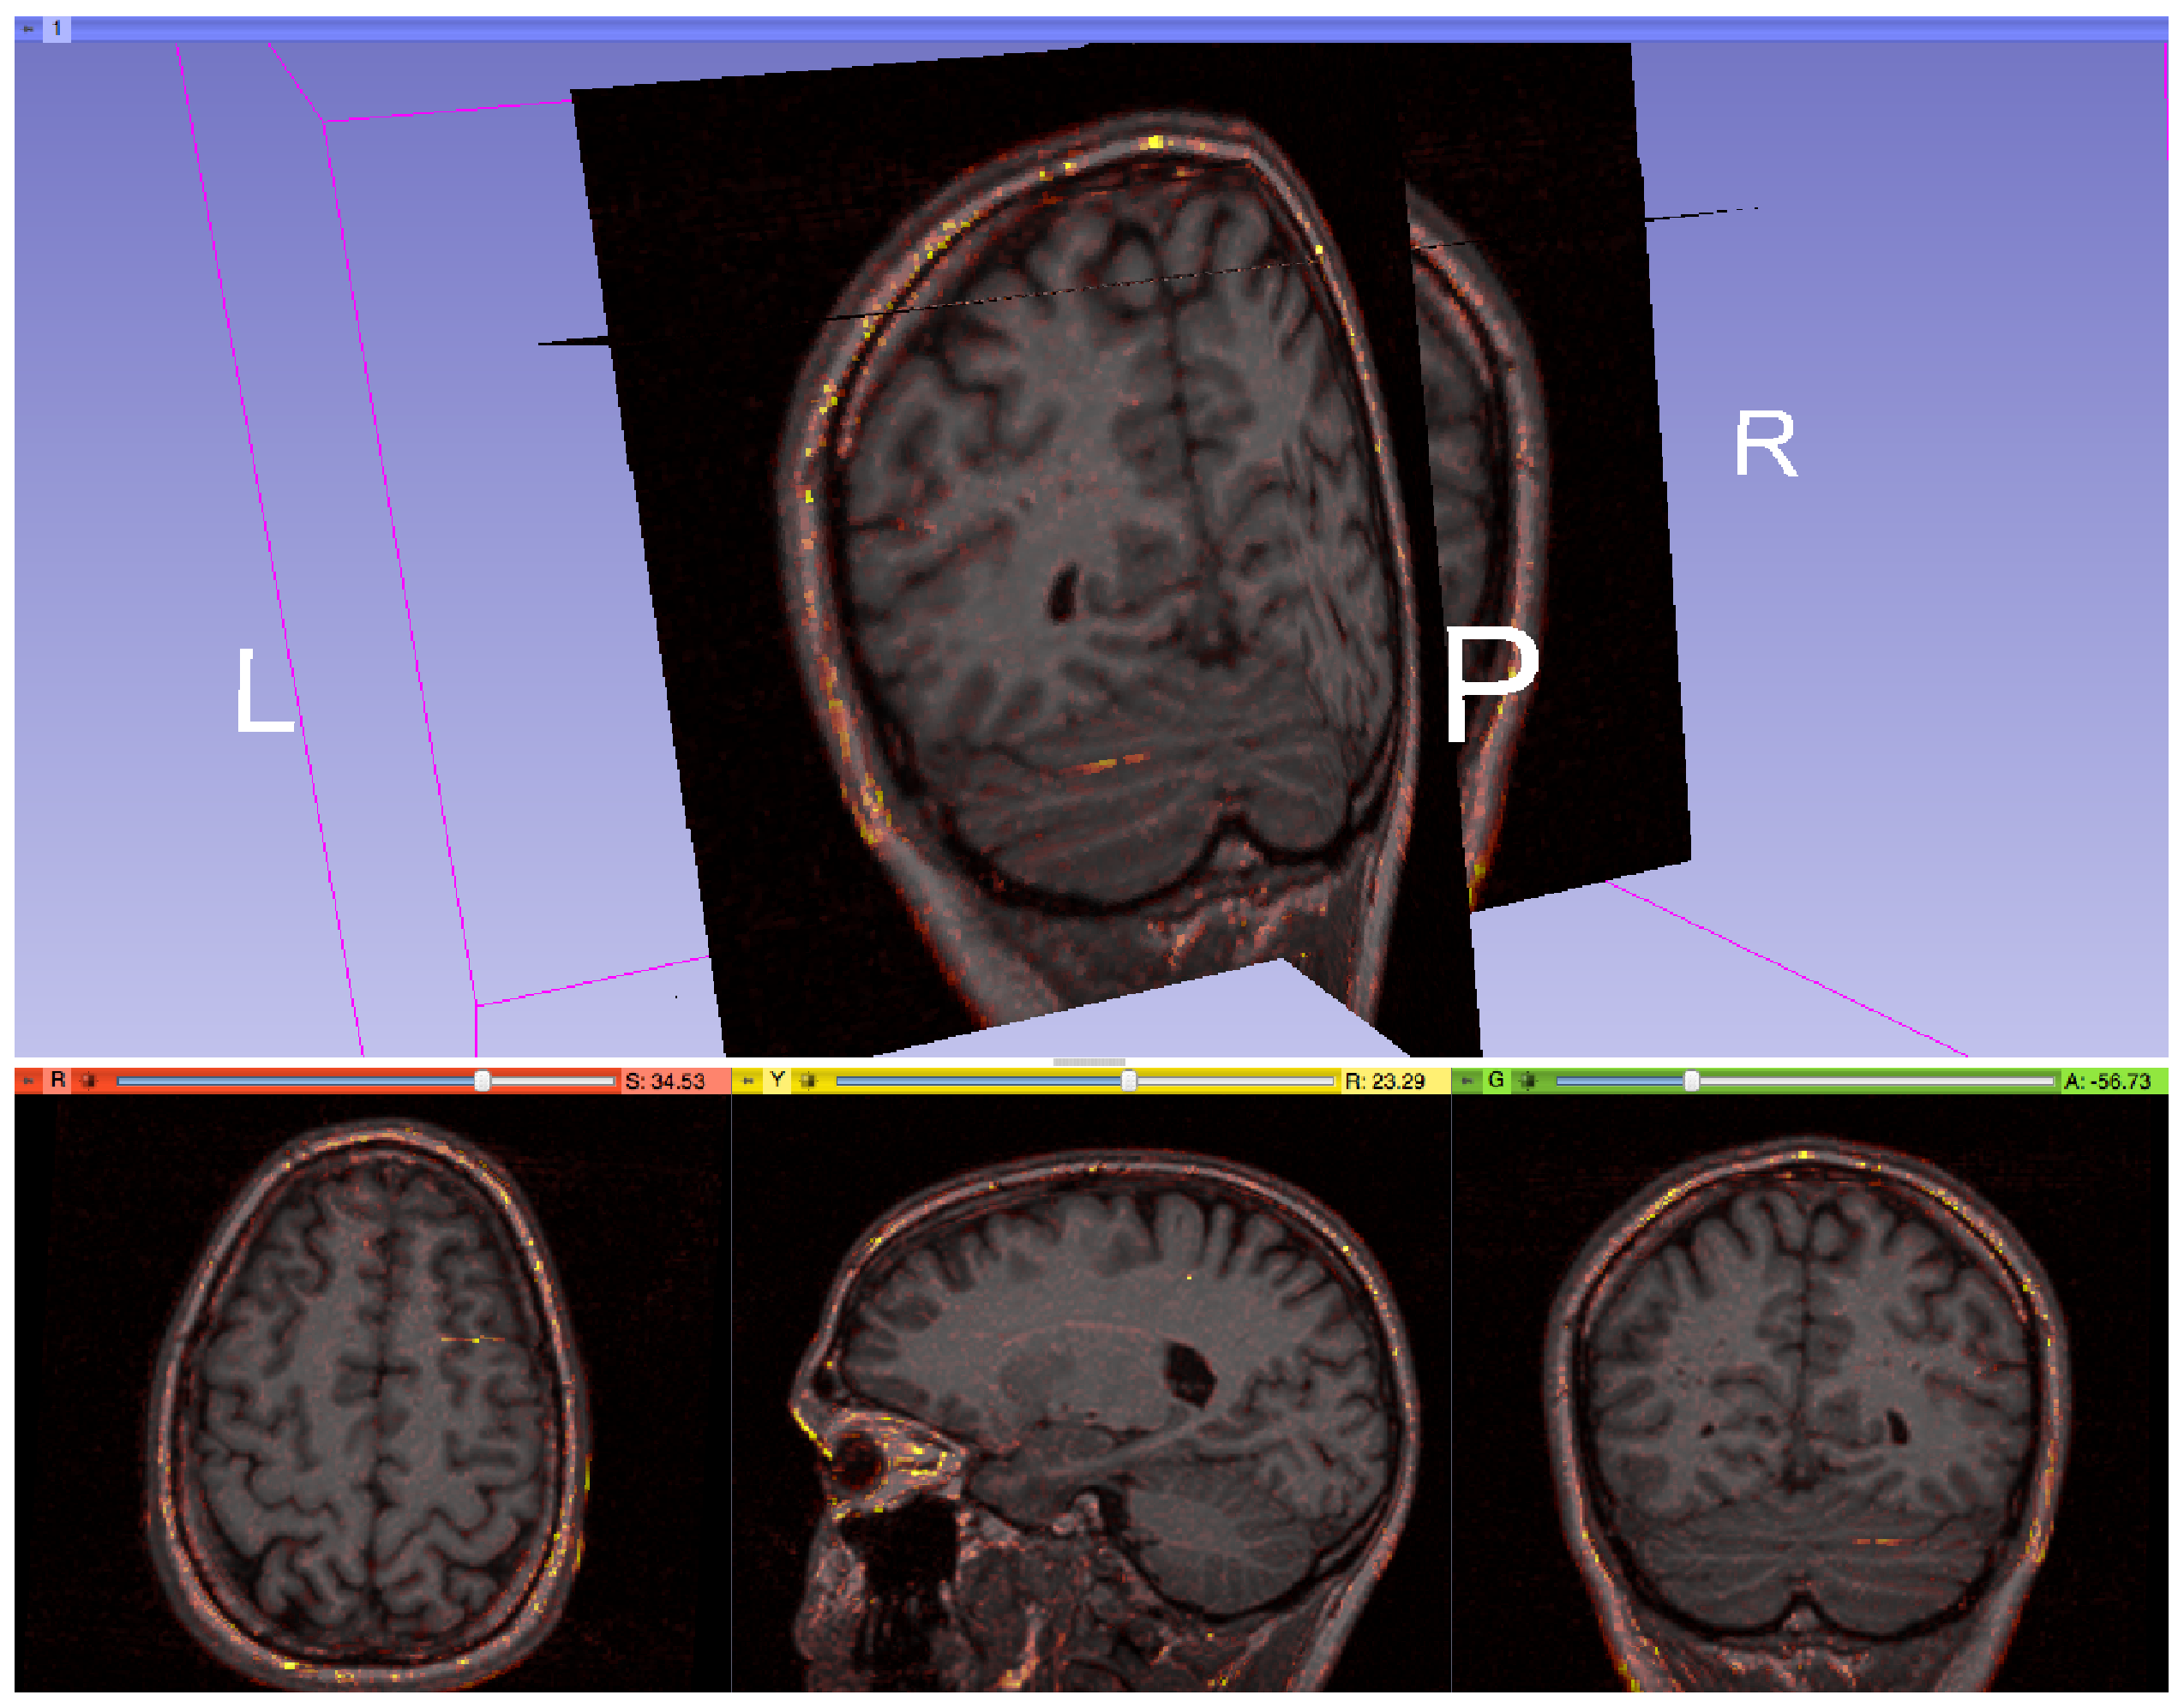
\includegraphics[scale=0.2]{/experiment_small/small_voxel2.eps}
  \caption{Artificial Small: Voxel-base method}
  \label{voxel_small2}
\end{figure}


\subsubsection{Tensor-based Method}
The result obtained is not very useful. It may be possible to find
some of the differences since we know their position in this
experiment. However, this would not be the case with real volumes as
it would be impossible to discern between real differences and those
produced by imperfections in the method.

The parameters used to obtain this result are:
\begin{description}
\item \textit{Deformation field smoothing sigma:} 3.5
\item \textit{Shrinkage percentage:} 70
\item \textit{Growth percentage:} 80
\end{description}

Note that in this case the parameter for deformation field smoothing
sigma is higher. This produced a smoother deformation field after the
registration, which improved the results to some extent; even though
the final result is still not good enough.

\begin{figure}[H]
  \centering
  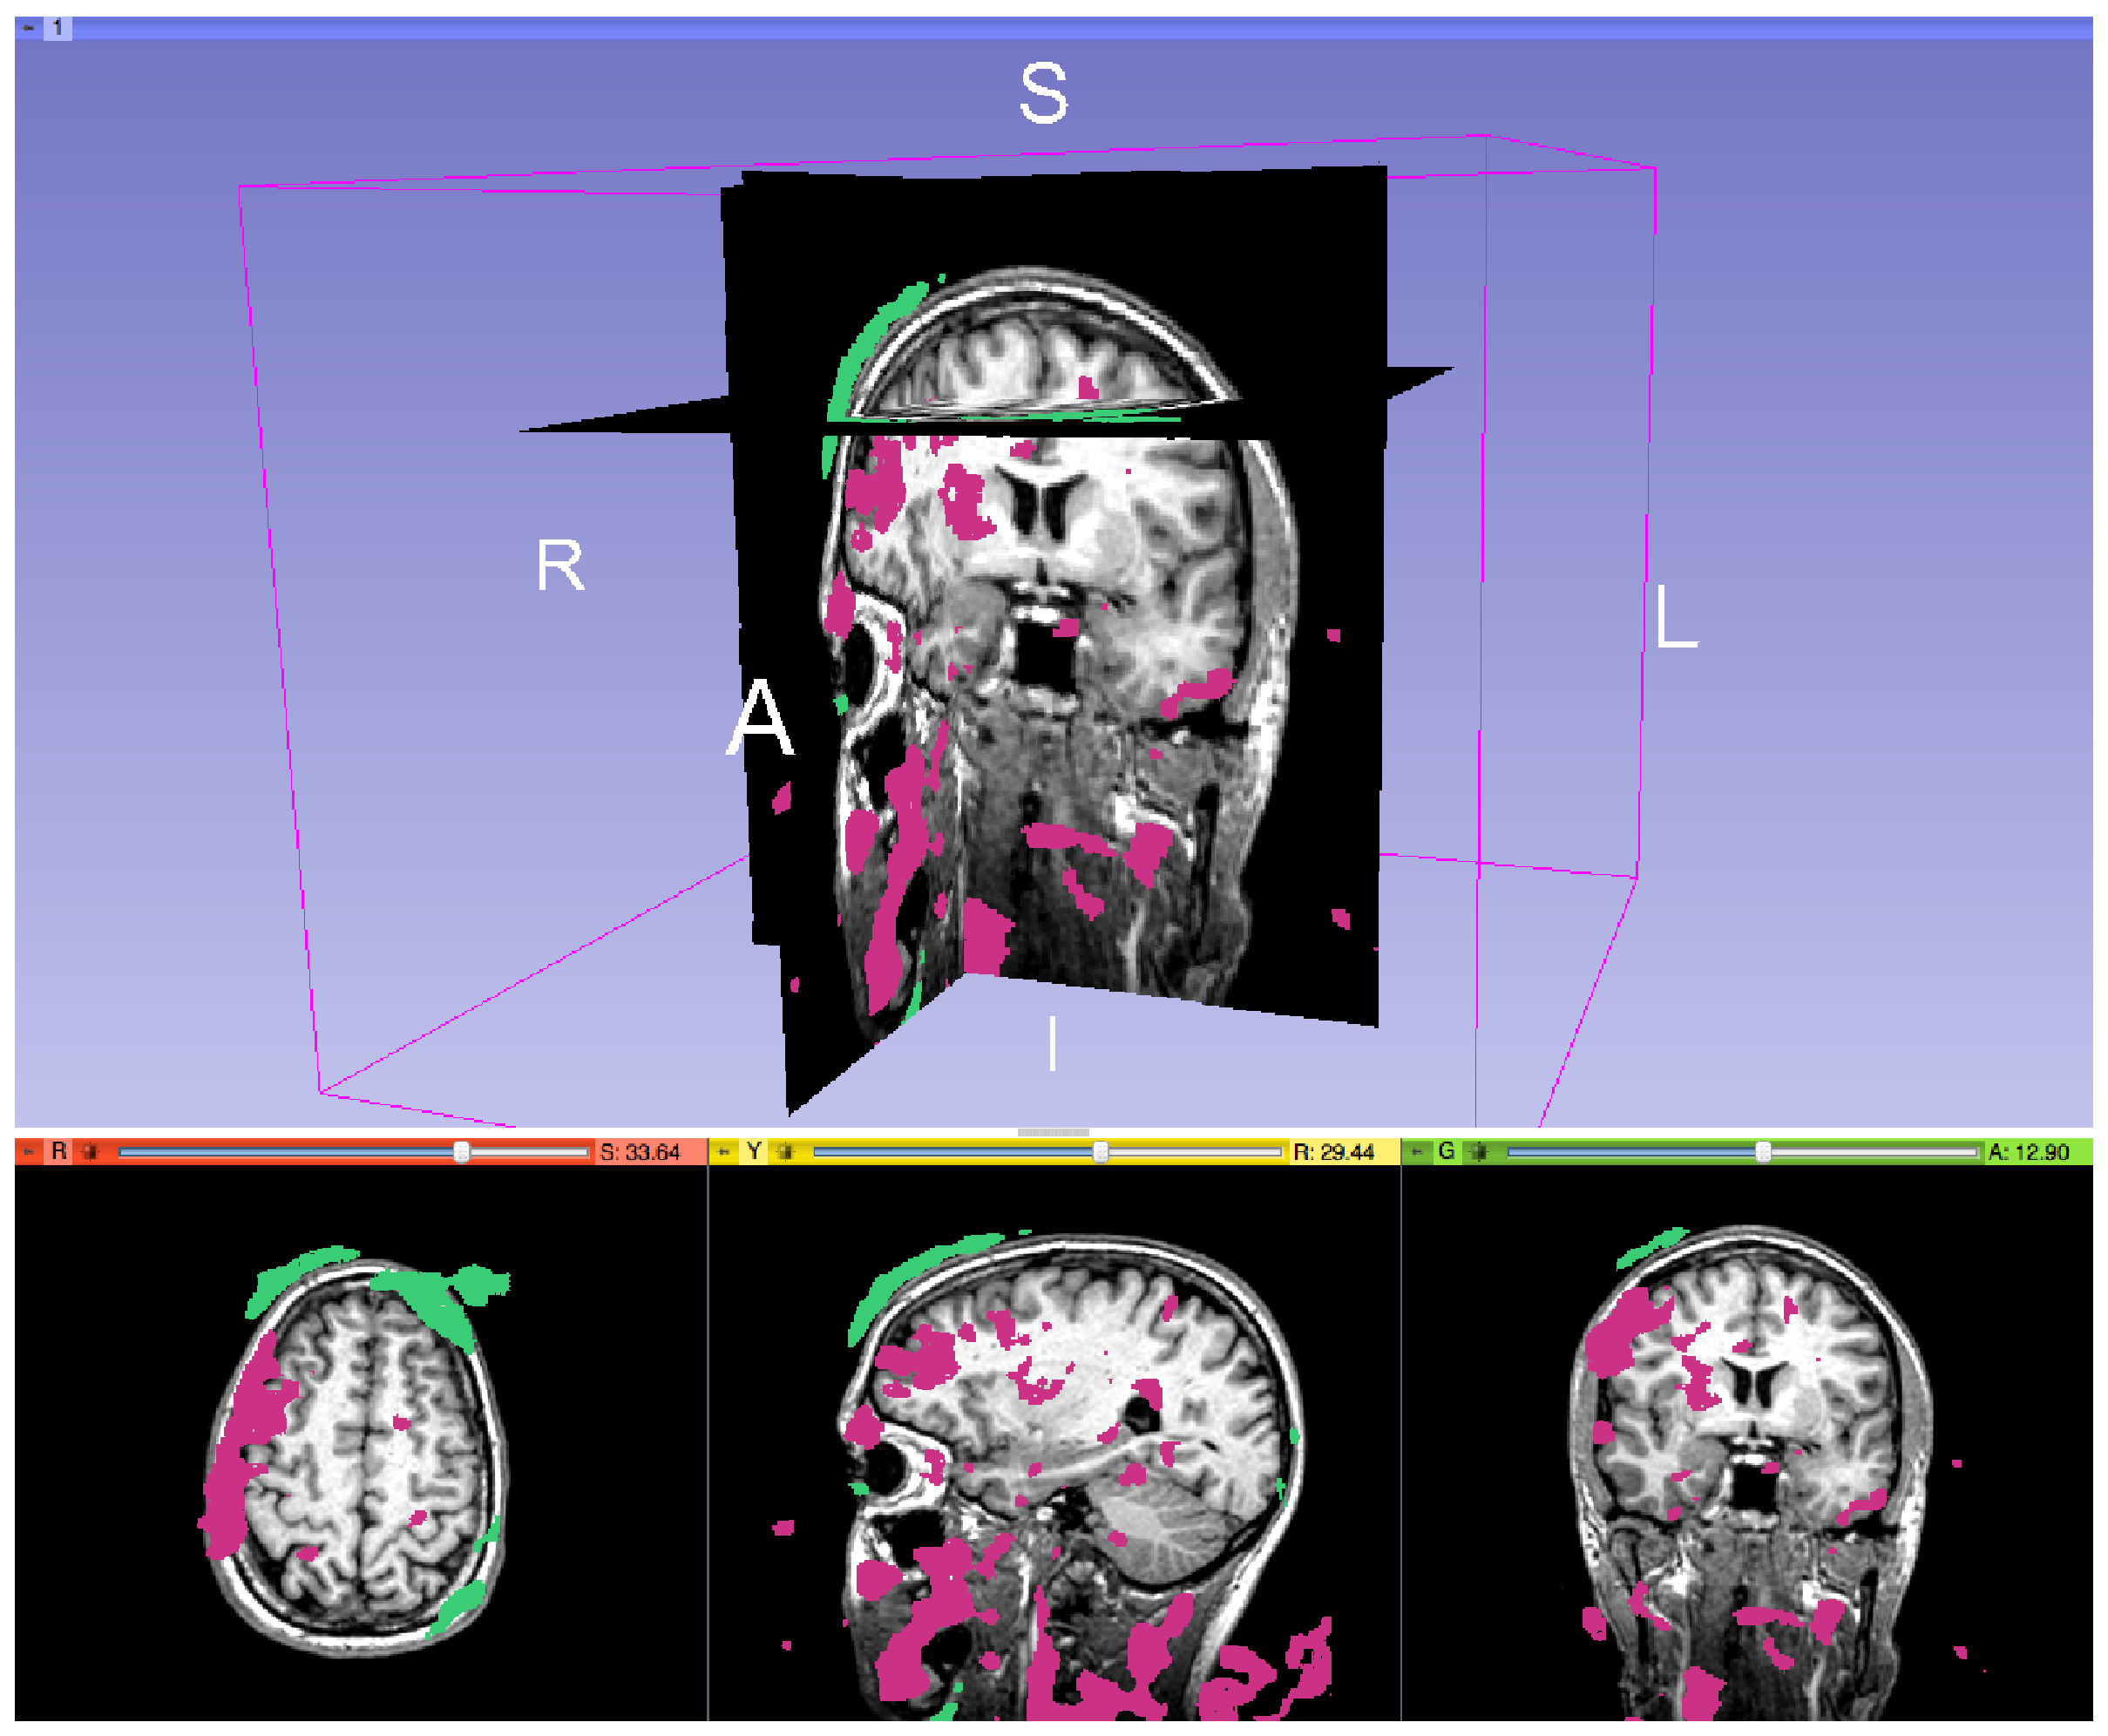
\includegraphics[scale=0.2]{/experiment_small/tensor_70-80_small1.eps}
  \caption{Artificial Small: Tensor-base method}
  \label{tensor_small1}
\end{figure}

Another angle of the result:

\begin{figure}[H]
  \centering
  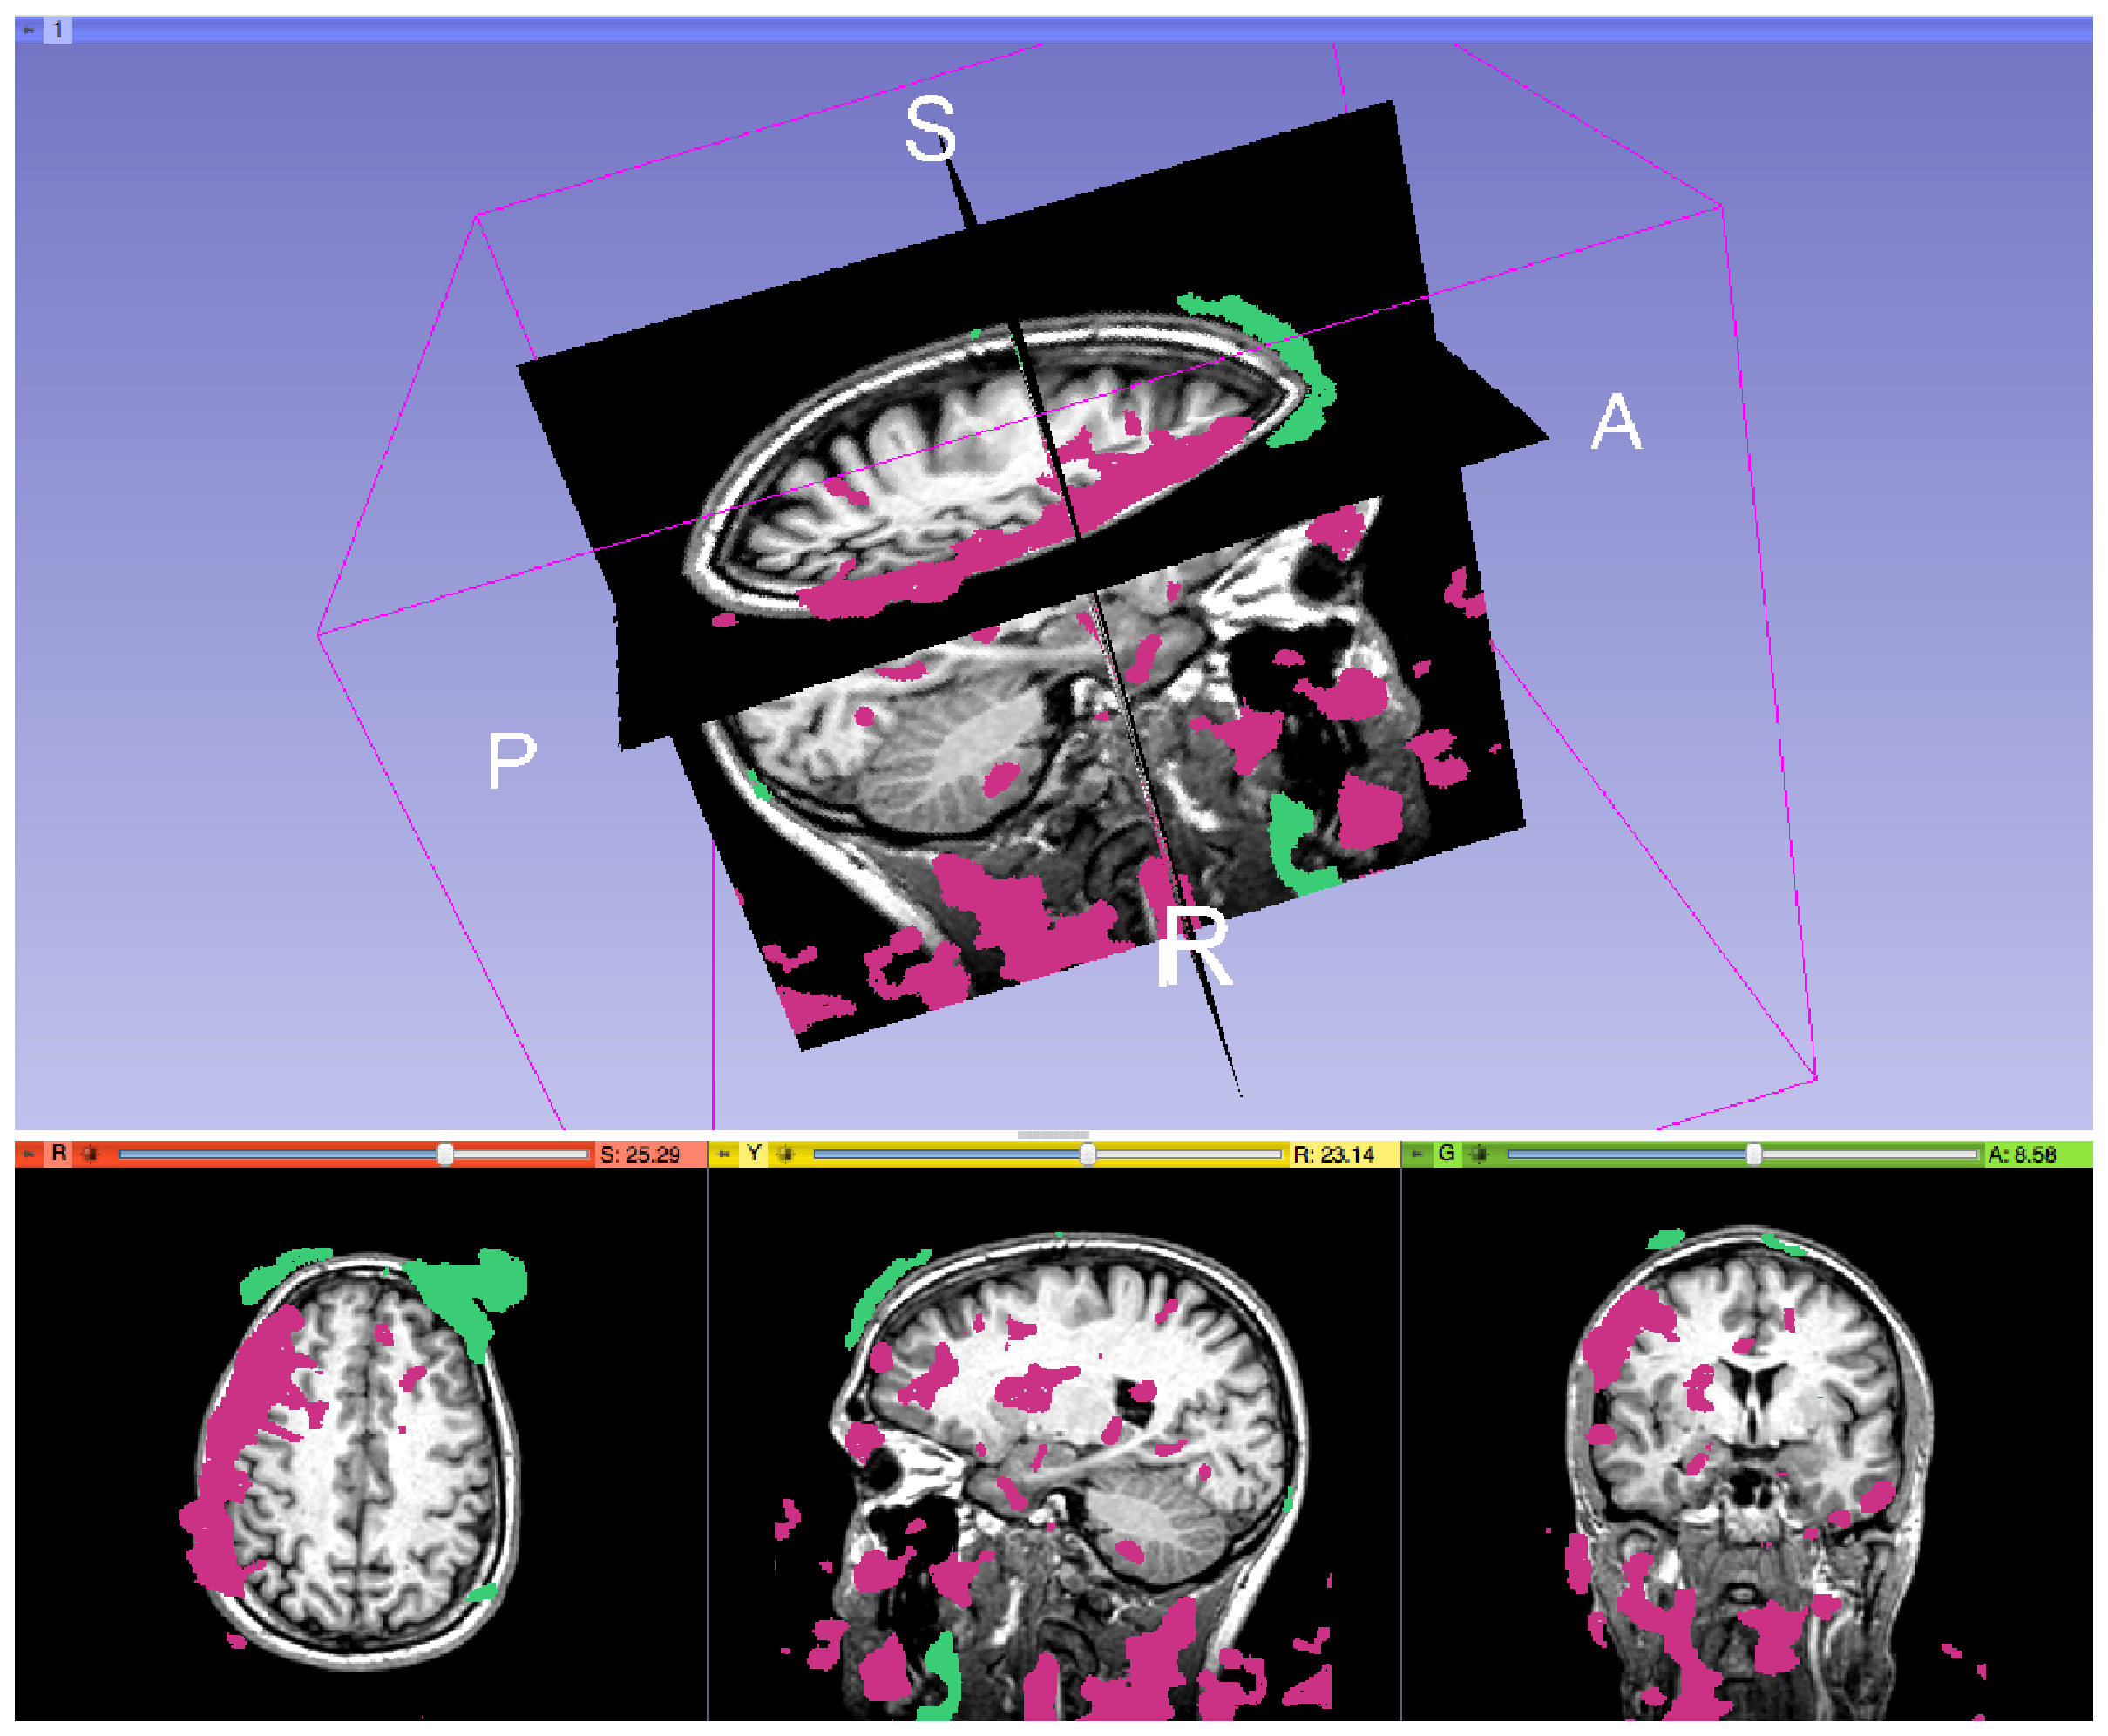
\includegraphics[scale=0.2]{/experiment_small/tensor_70-80_small2.eps}
  \caption{Artificial Small: Tensor-base method}
  \label{tensor_small2}
\end{figure}

\subsection{Size Increase of a Section}
A squared area inside the patient's brain was stretched out using an
image modification software, so that it seems that this area of the
brain increased in size.

The baseline volume without modifications can be seen in the following
image:

\begin{figure}[H]
  \centering
  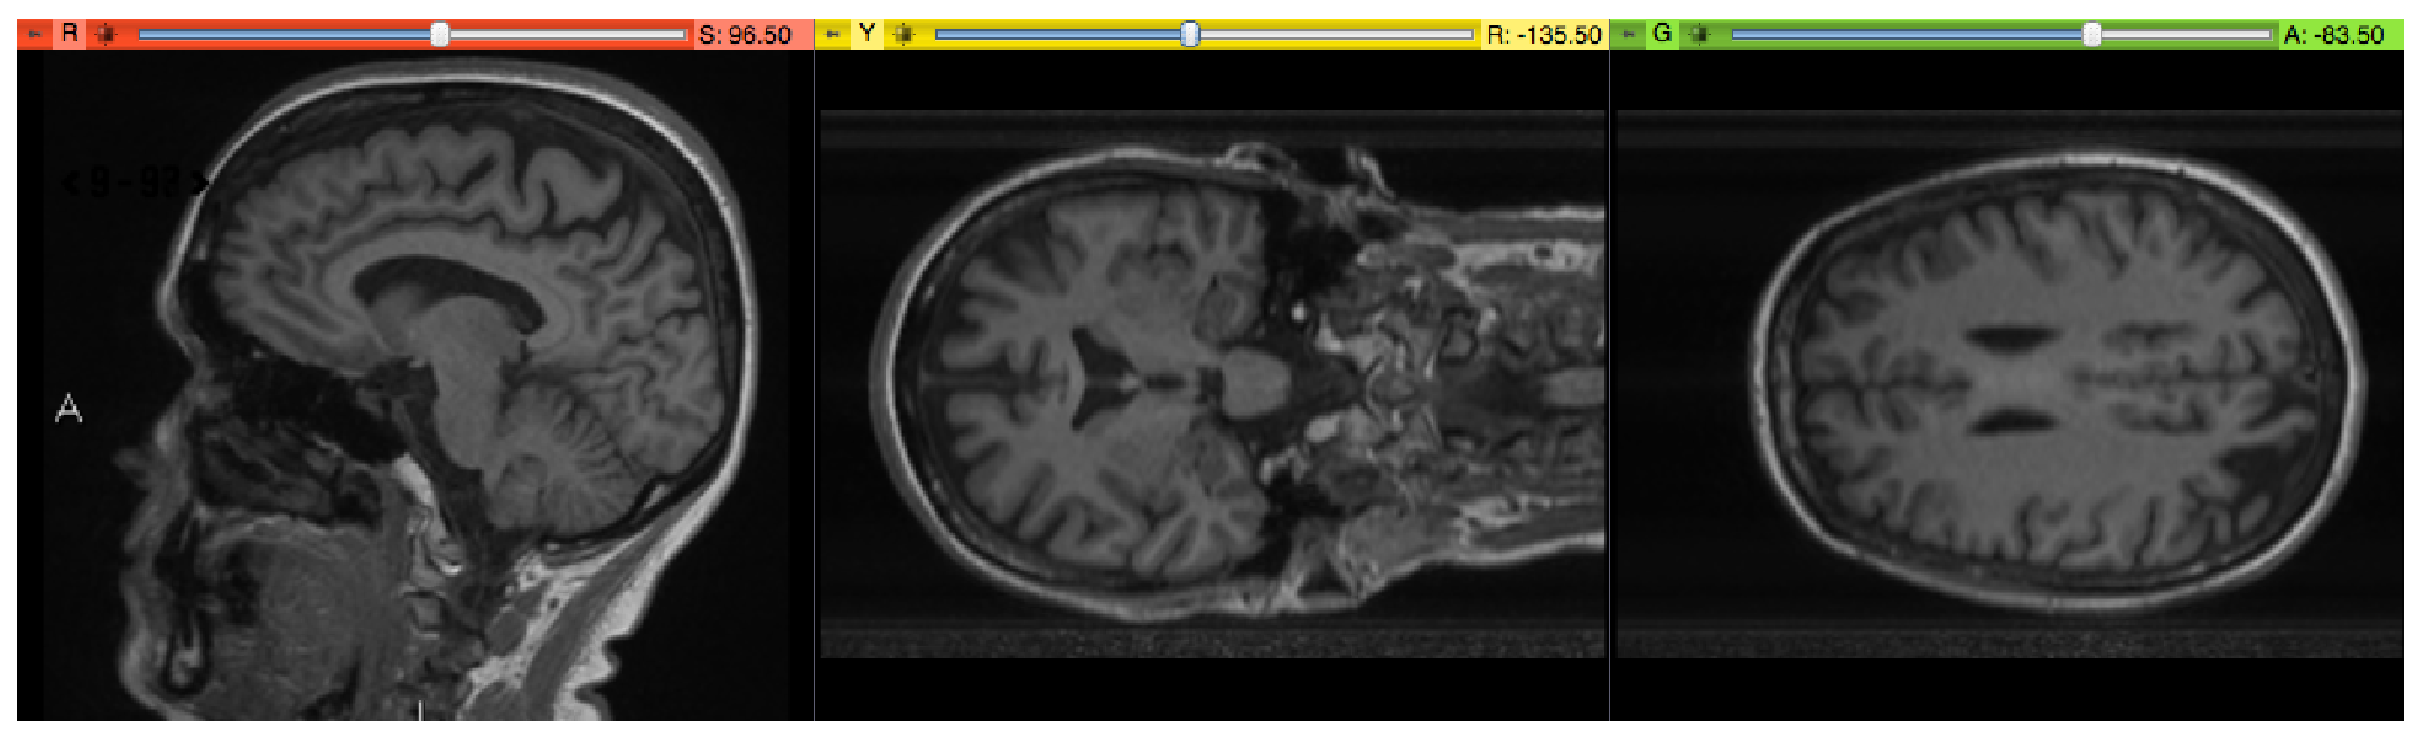
\includegraphics[scale=0.3]{/experiment_zoom/base.eps}
  \caption{Artificial Size increase: Baseline volume}
  \label{zoom_base}
\end{figure}

The next image shows the follow-up volume with the modifications
highlighted in red so that they might be easier to see:

\begin{figure}[H]
  \centering
  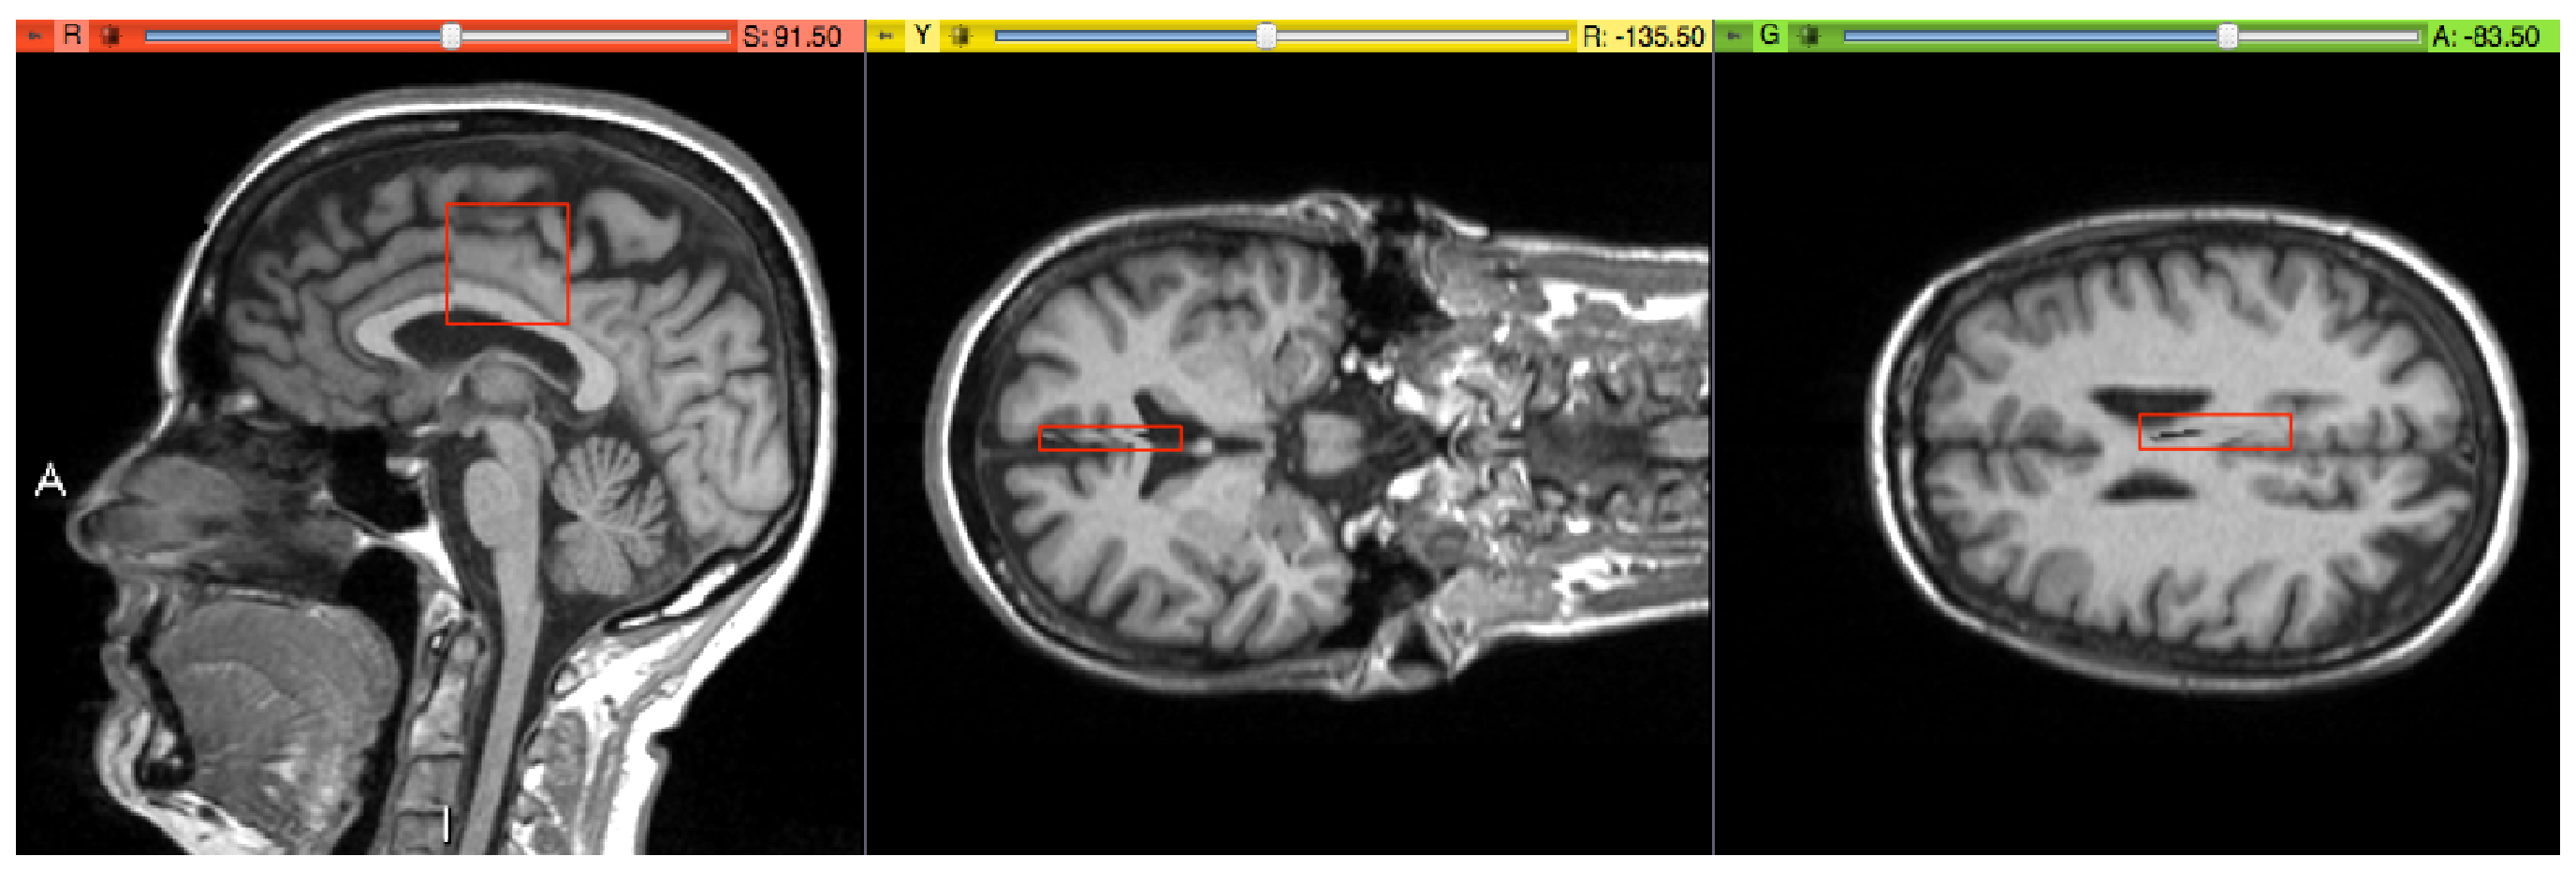
\includegraphics[scale=0.3]{/experiment_zoom/follow.eps}
  \caption{Artificial Size increase: Follow-up volume}
  \label{zoom_follow}
\end{figure}


\subsubsection{Voxel-based Method}
The result obtained with this method is quite good, the brightest
areas definitely correspond with the area of size increase. Even the
squared shape of the area can be observed in the resulting volume.

\begin{figure}[H]
  \centering
  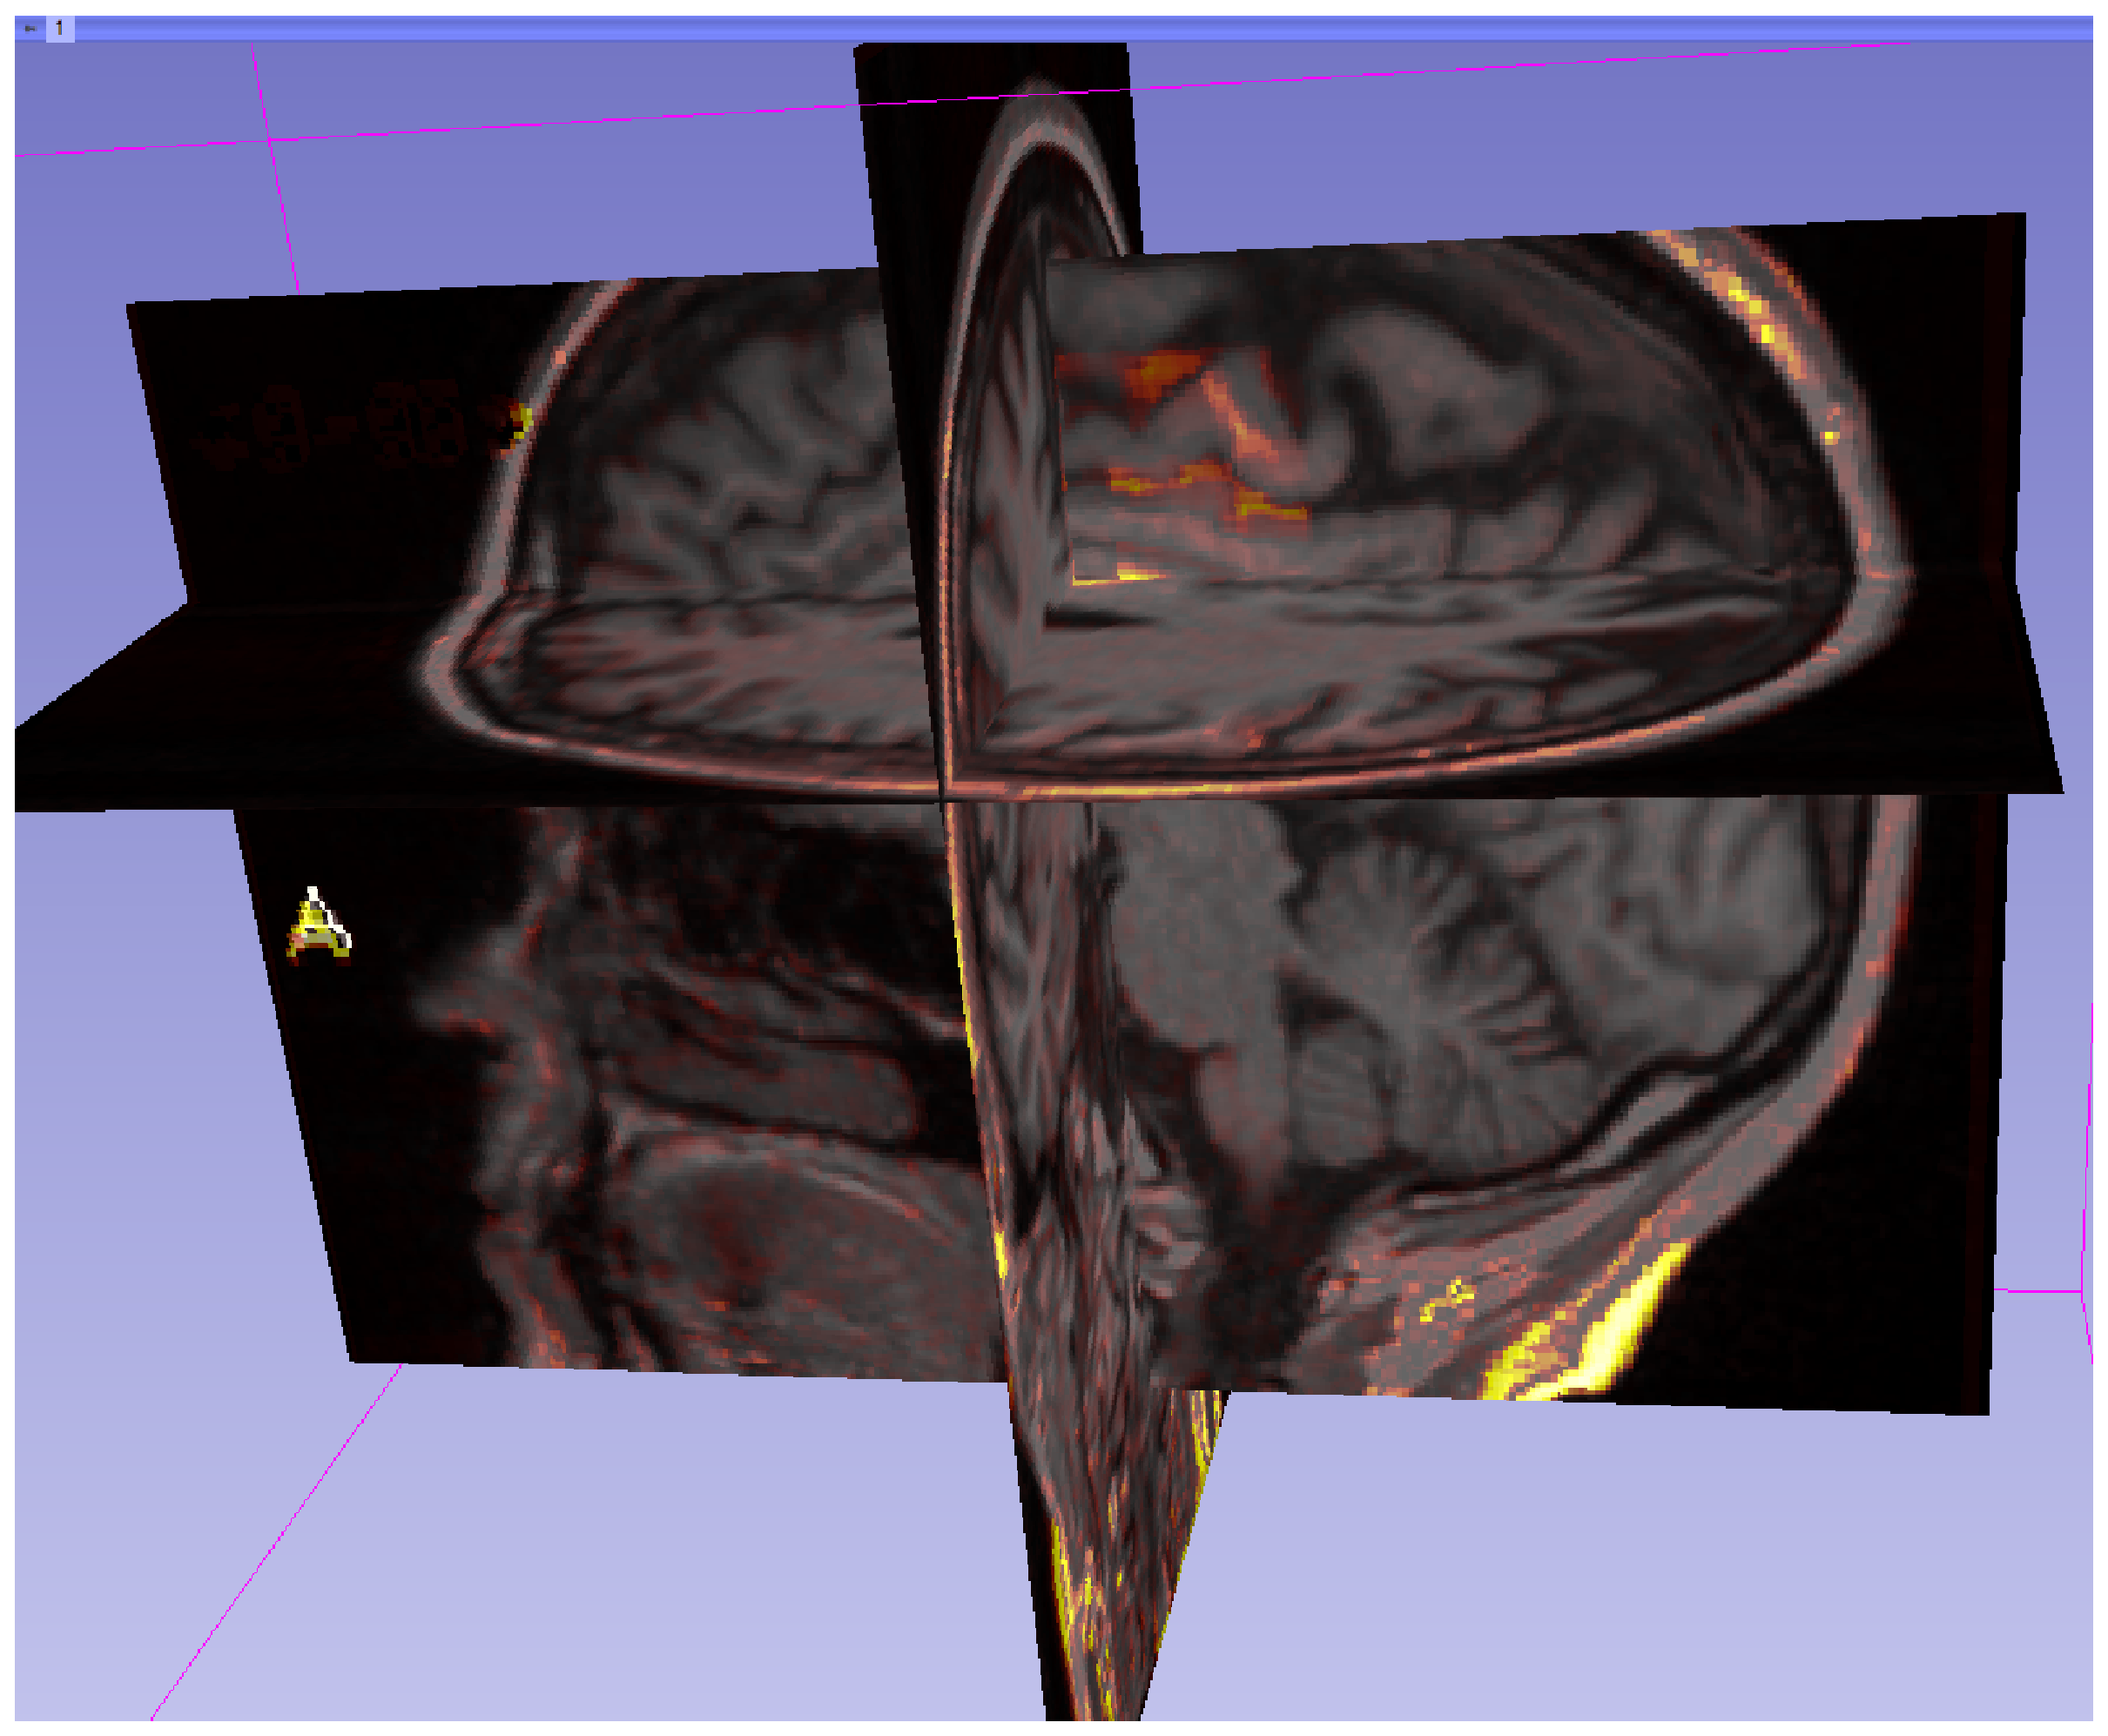
\includegraphics[scale=0.2]{/experiment_zoom/zoom_voxel1.eps}
  \caption{Artificial Size increase: Voxel-based method}
  \label{zoom_voxel1}
\end{figure}

Another angle of the result:

\begin{figure}[H]
  \centering
  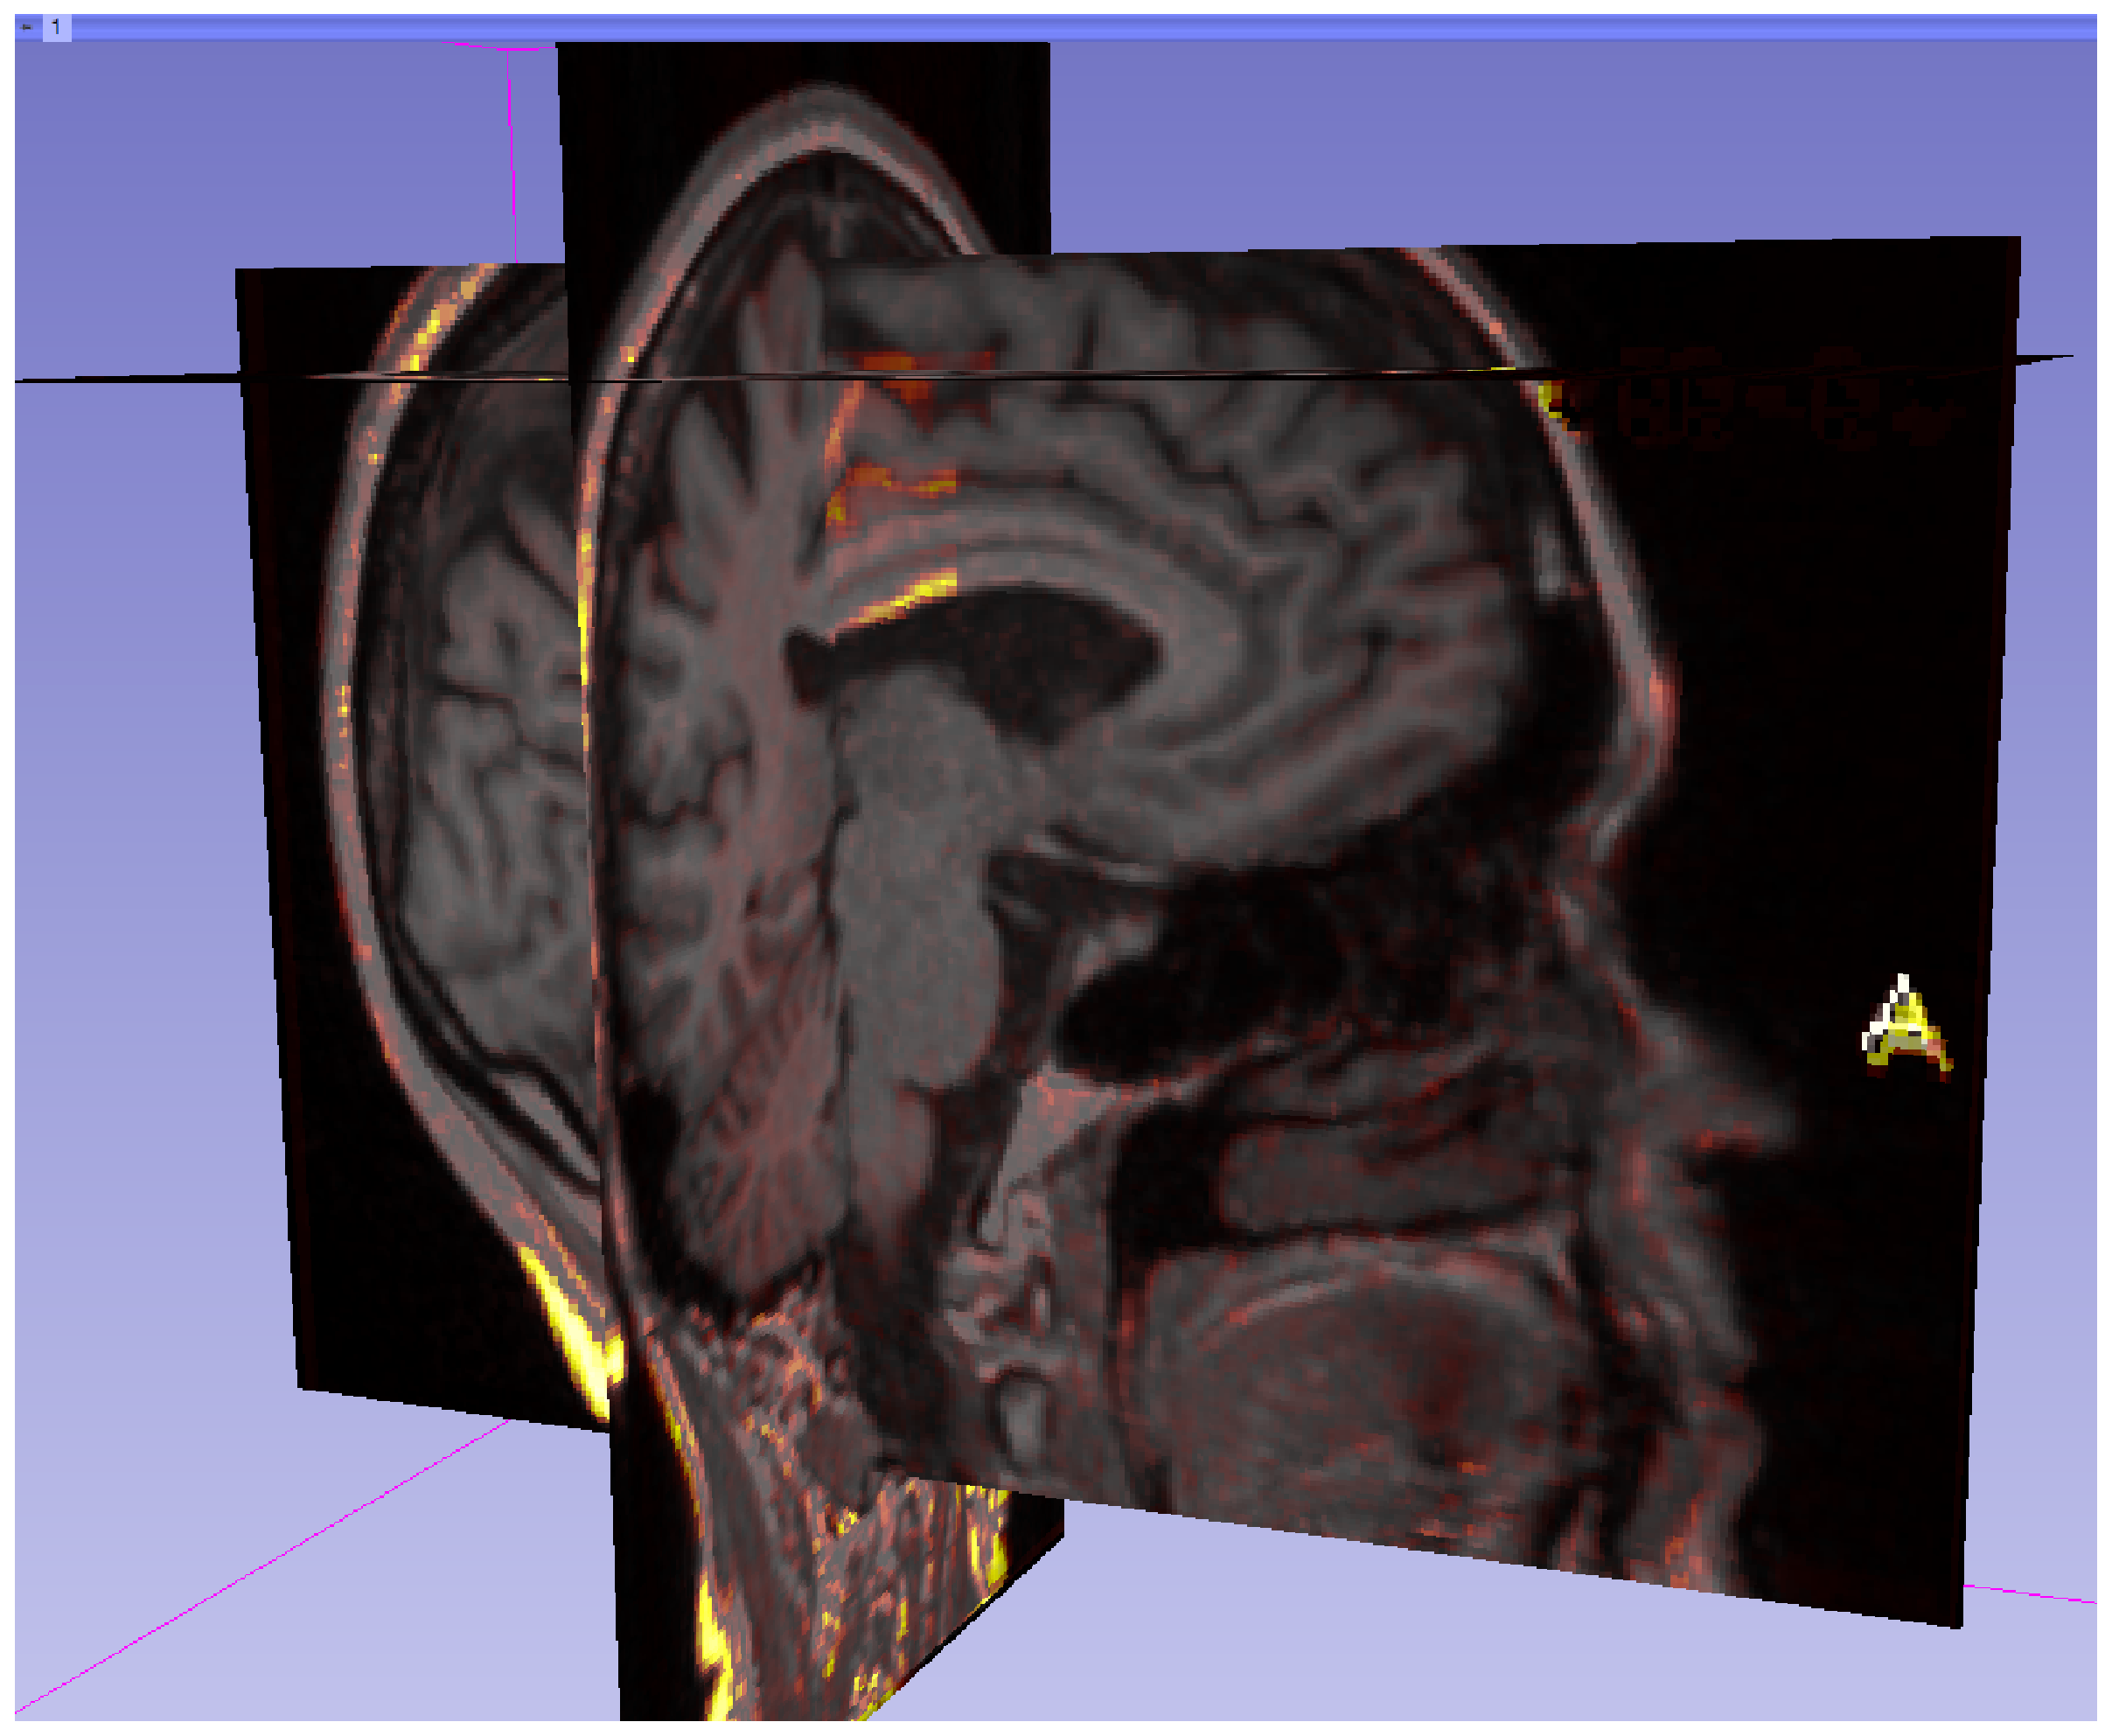
\includegraphics[scale=0.2]{/experiment_zoom/zoom_voxel2.eps}
  \caption{Artificial Size increase: Voxel-based method}
  \label{zoom_voxel2}
\end{figure}


\subsubsection{Tensor-based Method}
Even though it would make sense for the tensor-based method to produce
better results in this test, the final label map is unable to show the
differences added and it shows quite a large amount of noise detected
as differences.

During this specific case the value of the \textit{deformation field
  smoothing sigma} makes a big difference in the final volume.  It
seems that the added size increase only produces a very small change
in the deformation field resulting from the registration; as a
consequence, the deformation field obtained with a smoothing sigma of
$2.5$ is too smooth and the differences we are looking for disappear.

The following image shows this result with 70 and 90 as the
percentages of shrinkage and growth respectively:

\begin{figure}[H]
  \centering
  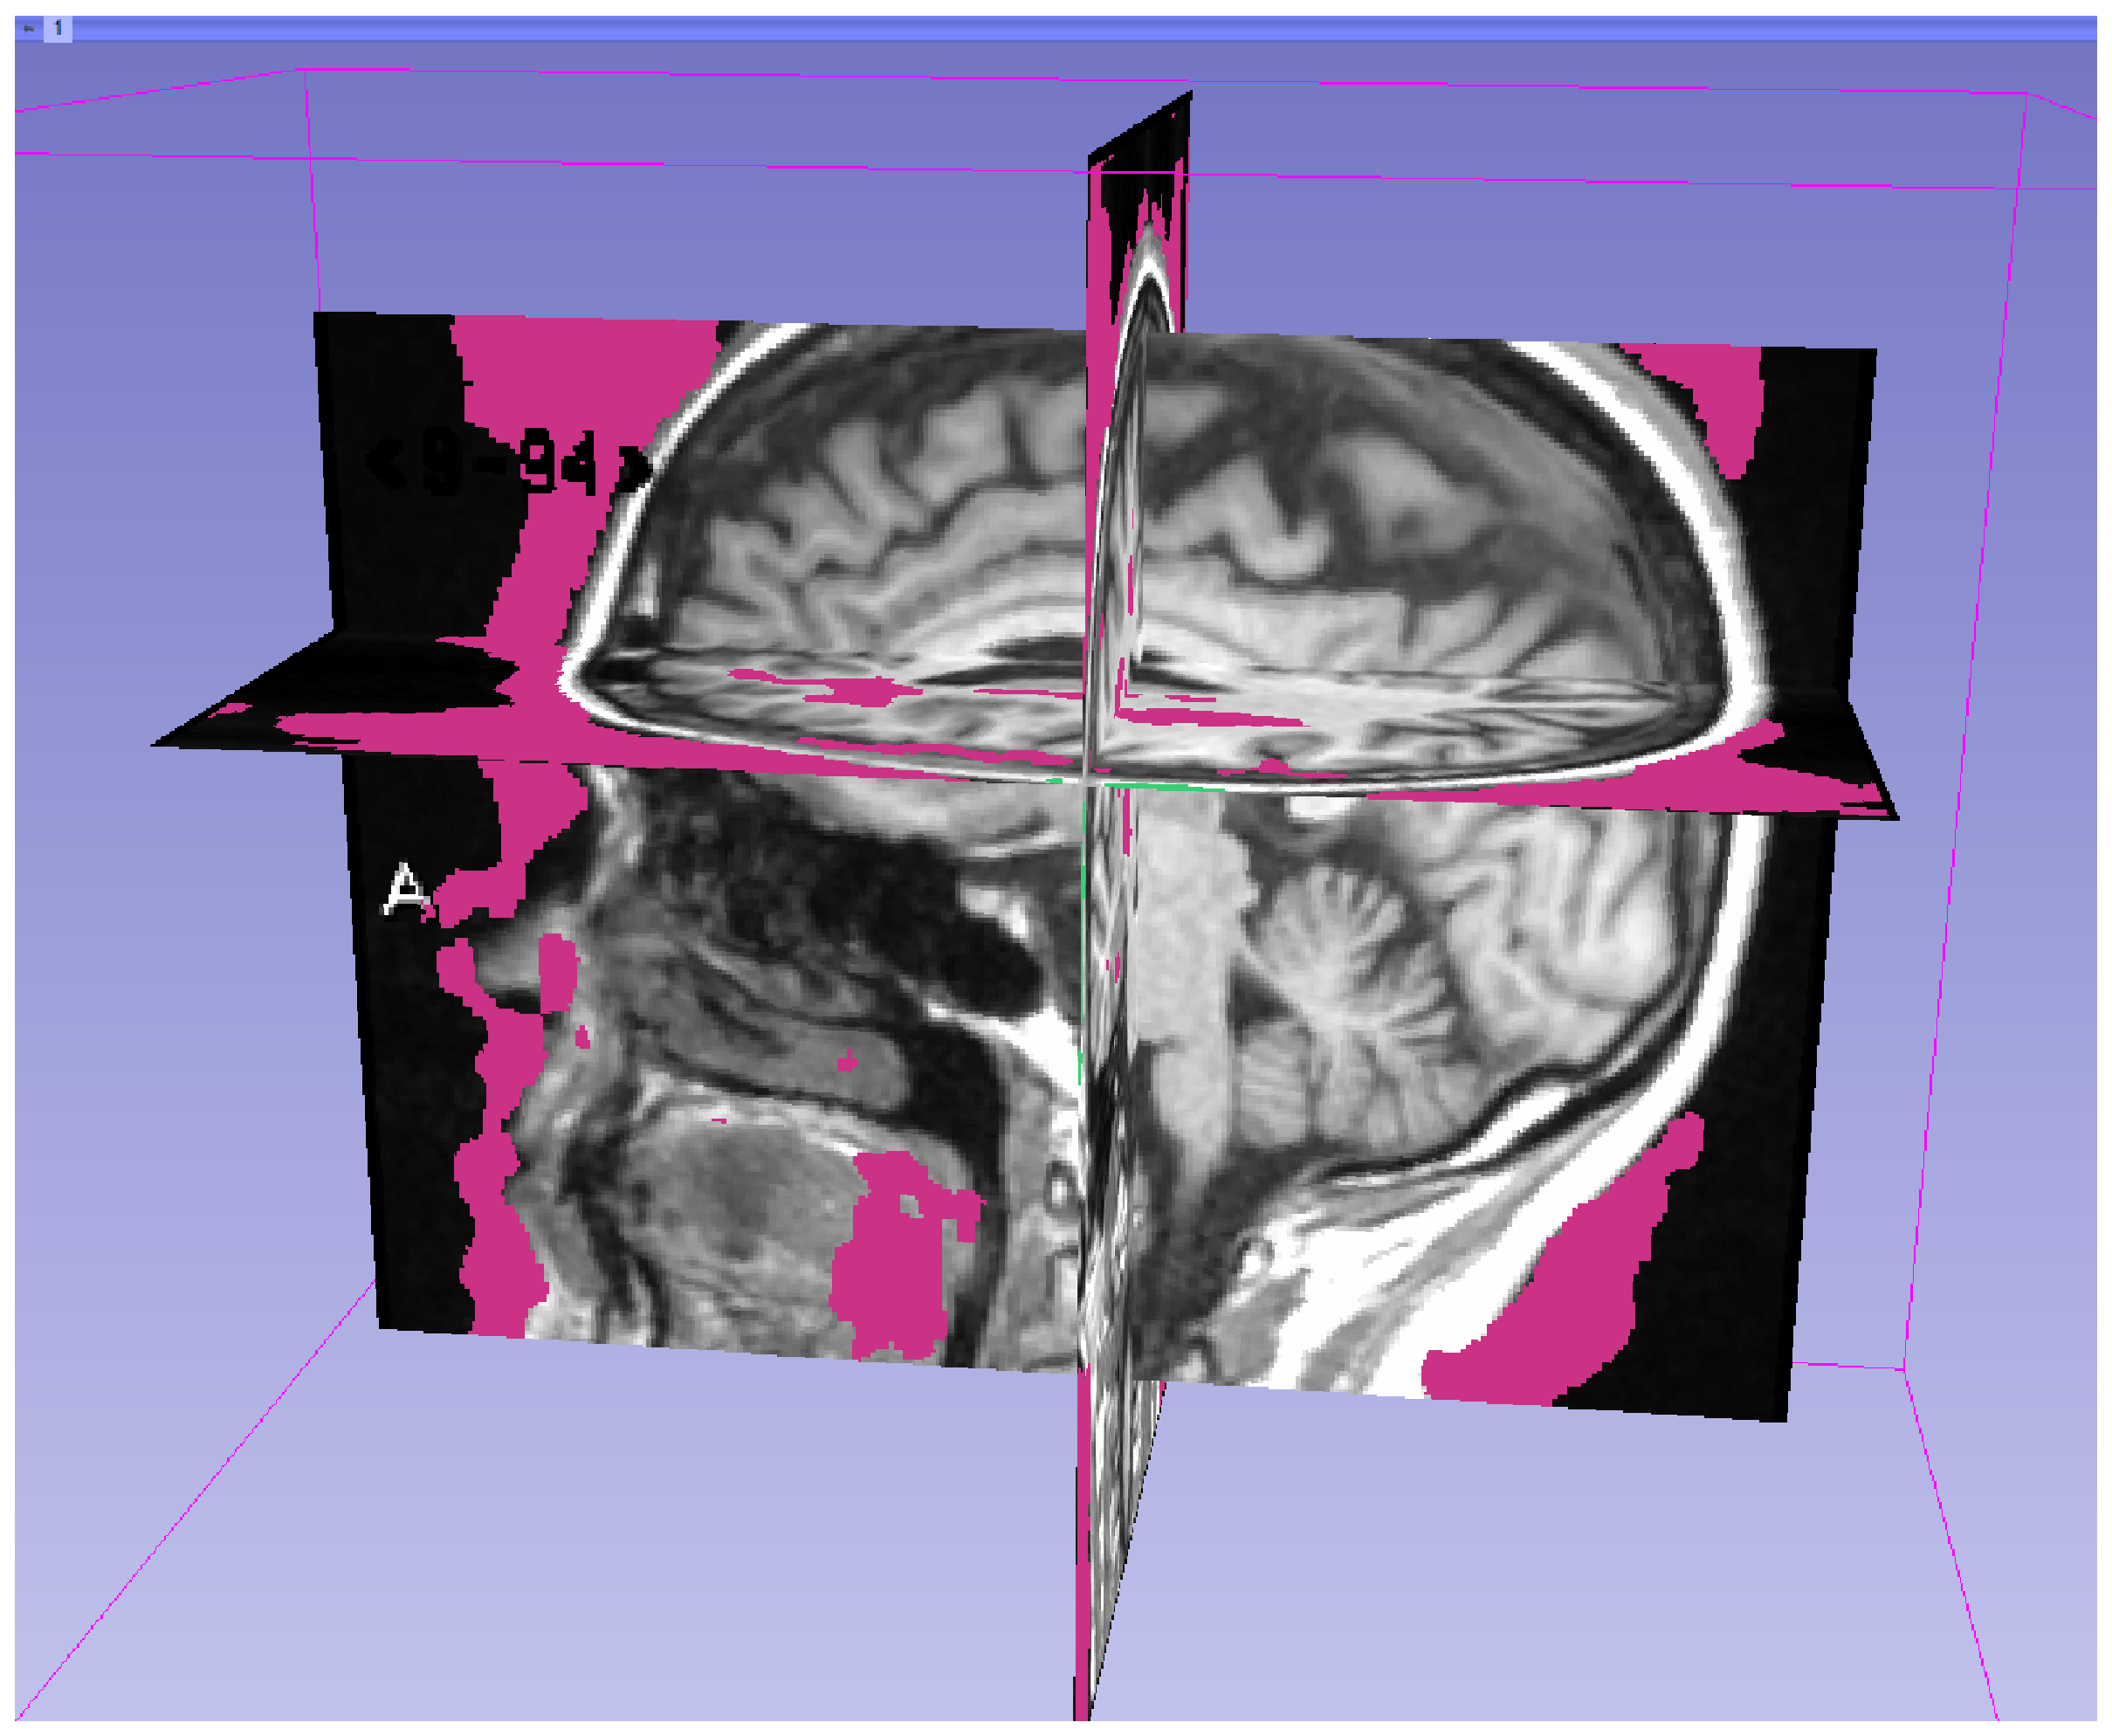
\includegraphics[scale=0.2]{/experiment_zoom/zoom_tensor_DF2-5_70_90.eps}
  \caption{Artificial Size increase: Tensor-based, Smoothing sigma of 2.5}
  \label{zoom_tensor1}
\end{figure}

If the \textit{deformation field smoothing sigma} is decreased to
$1.0$, the deformation field seems to retain some of the interesting
information. But the result still has a lot of noise.

The following image shows this result with 70 and 85 as the
percentages of shrinkage and growth respectively:

\begin{figure}[H]
  \centering
  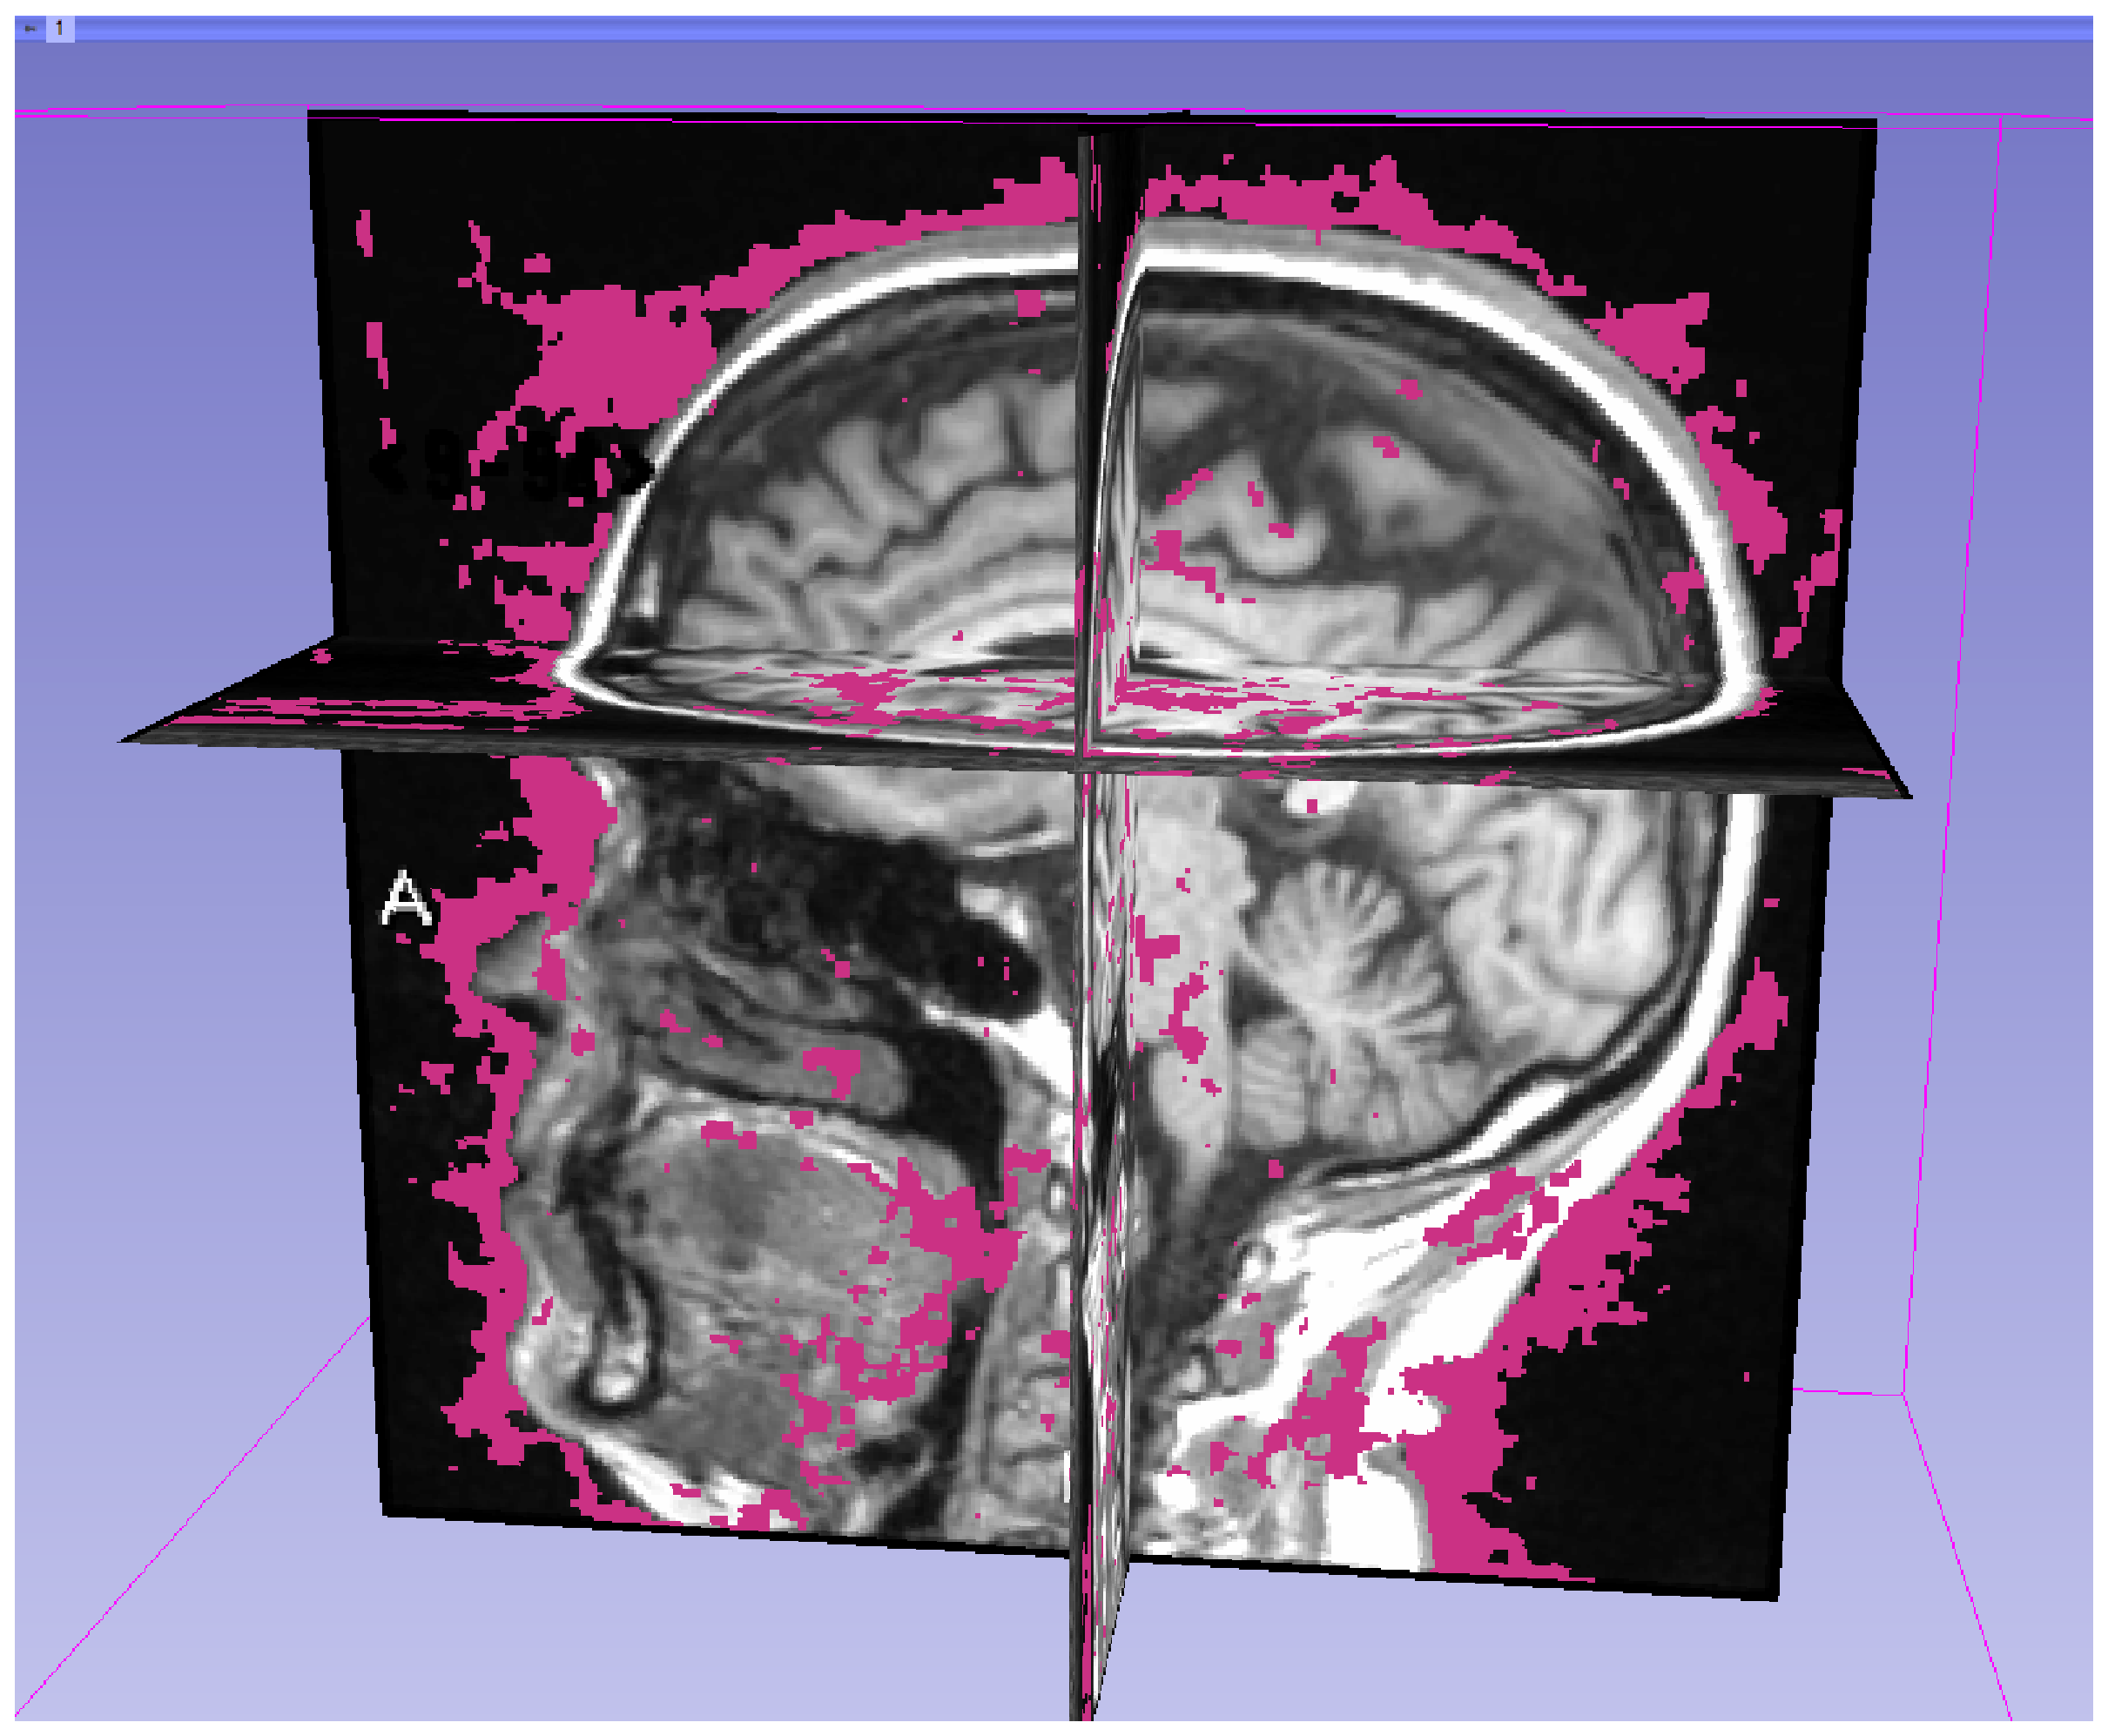
\includegraphics[scale=0.2]{/experiment_zoom/zoom_tensor_DF1_70_85.eps}
  \caption{Artificial Size increase: Tensor-based, Smoothing sigma of 1.0}
  \label{zoom_tensor2}
\end{figure}


\section{Real Differences Results}

\subsection{Patient 1}
This patient presents small differences in the parietal lobe, the
differences can be seen as red lines in the voxel-based method's result
and pink or green areas in the tensor-based method's result.

\subsubsection{Voxel-based Method}
The registration method used was \textit{Affine registration}.

\begin{figure}[H]
  \centering
  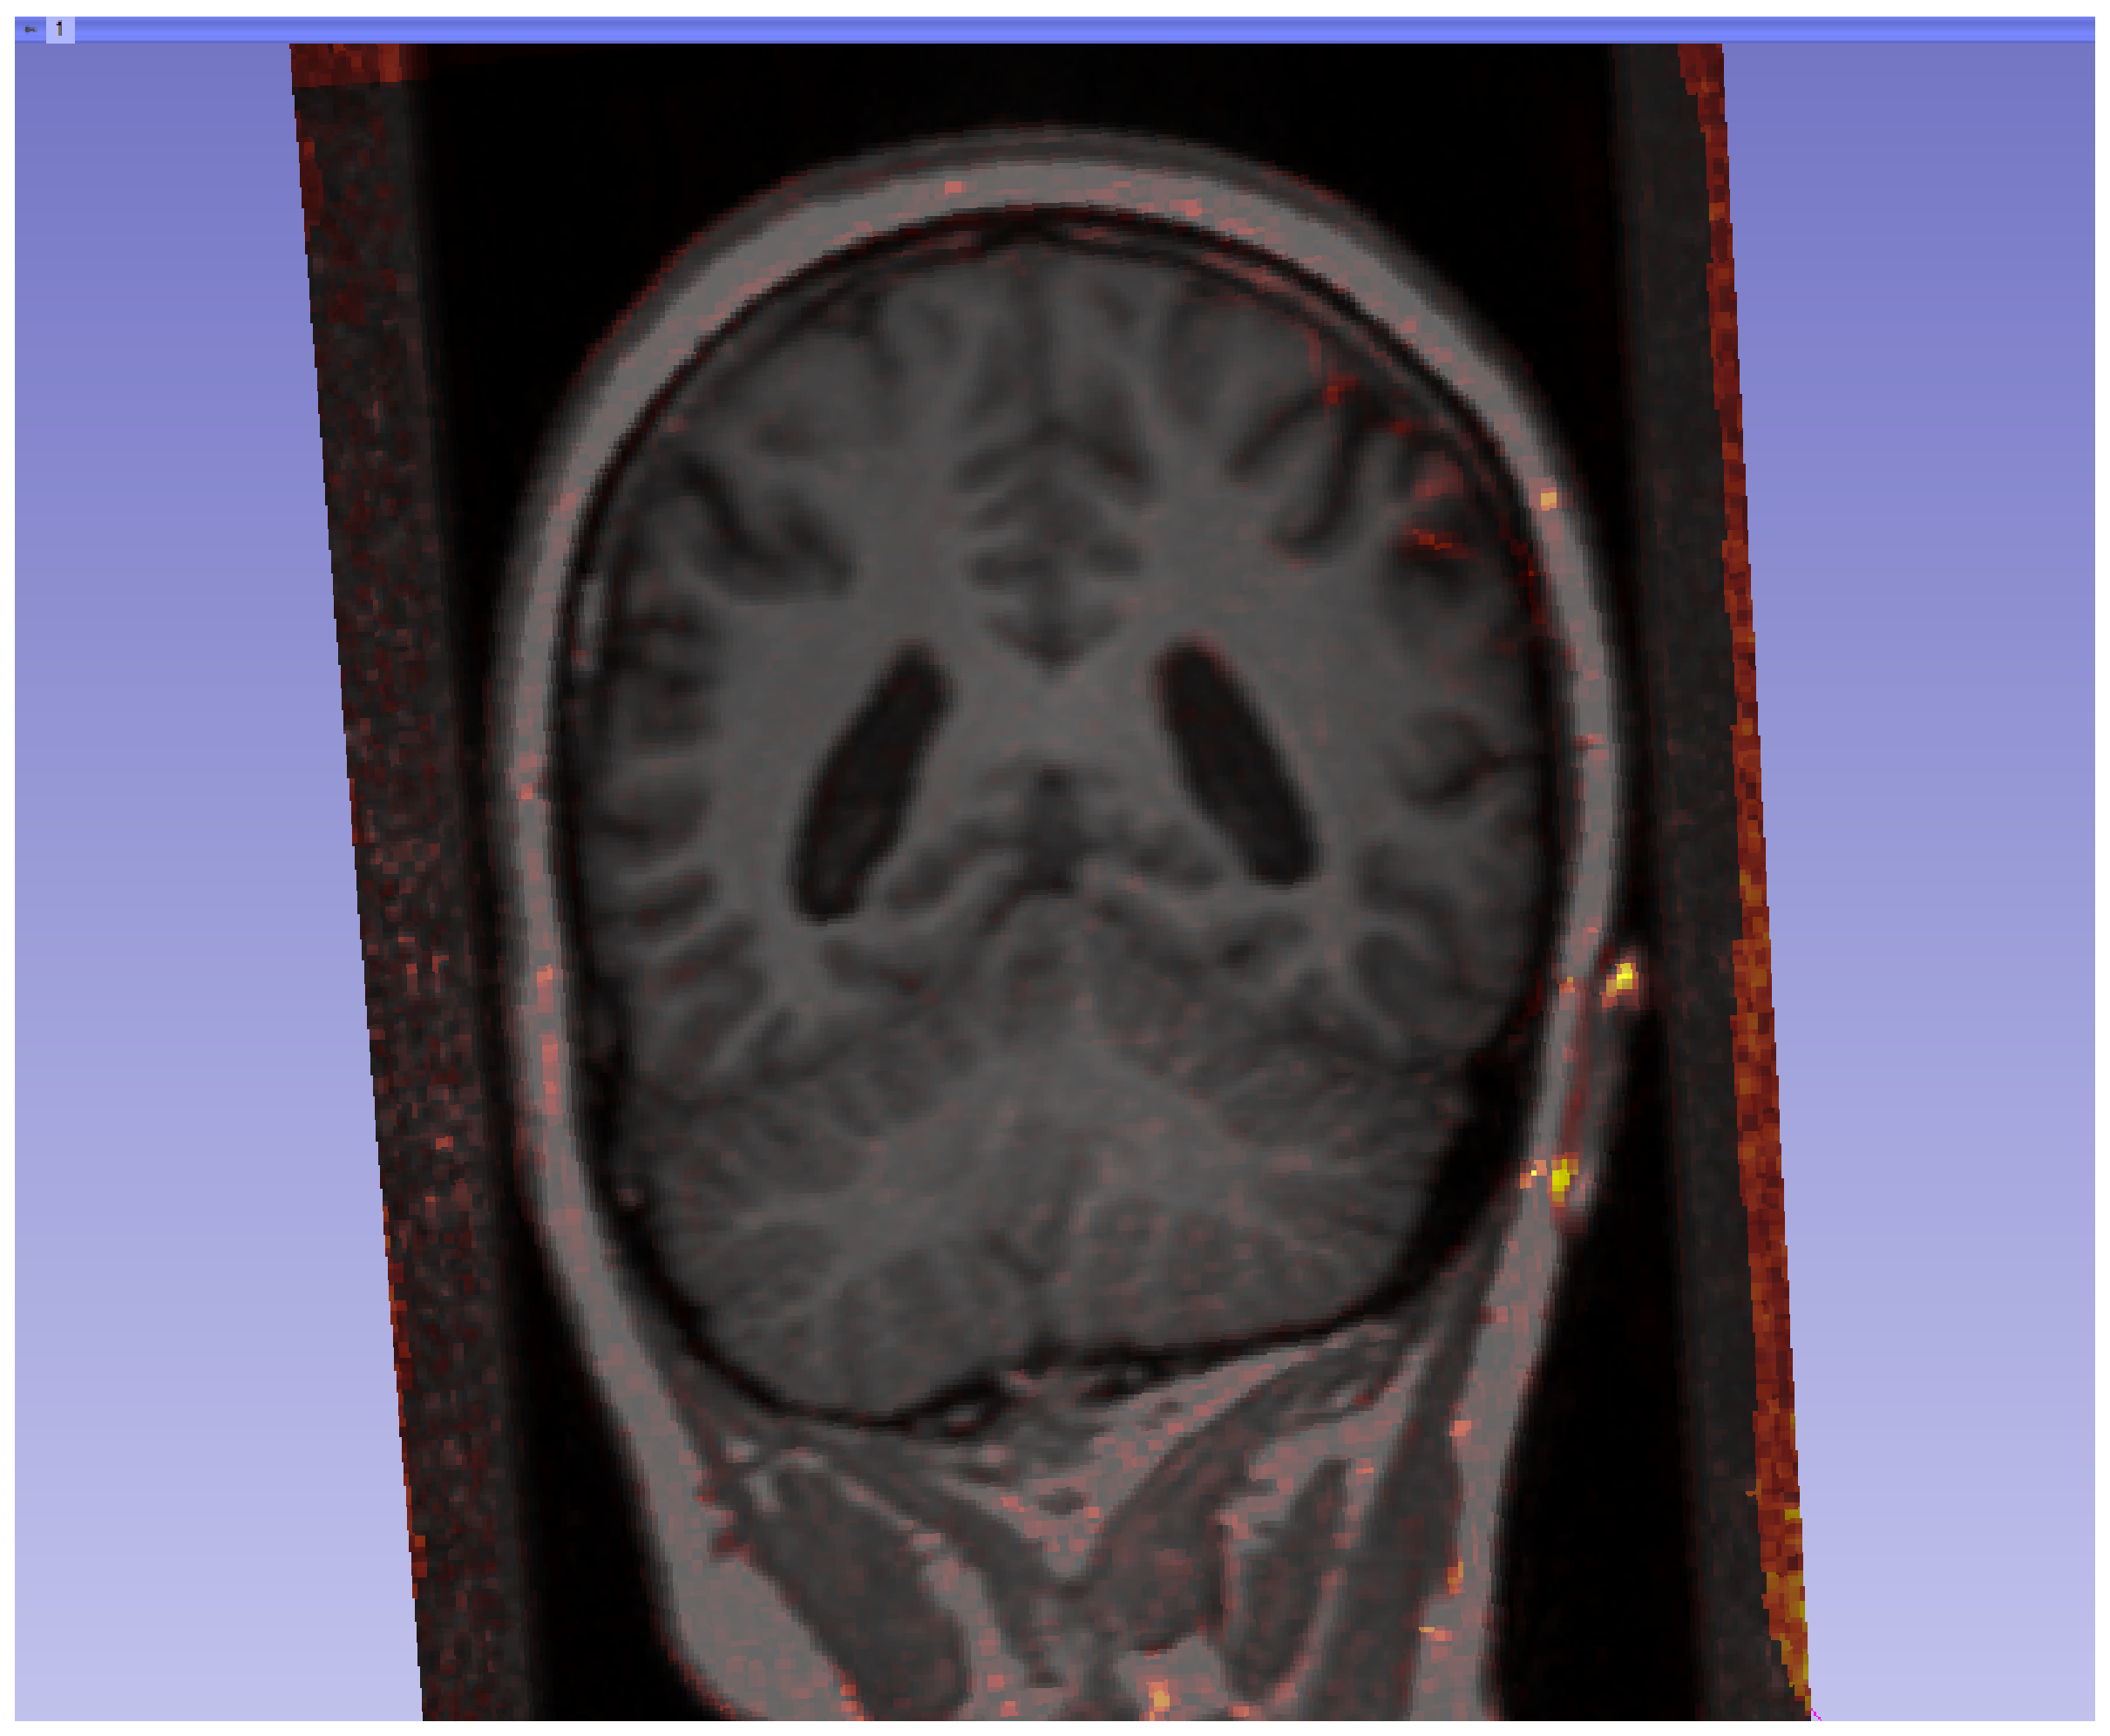
\includegraphics[scale=0.2]{/experiment_CL_P1/CL_Coronal.eps}
  \caption{Voxel-based method. Patient 1: Coronal plane}
  \label{CL_Coronal}
\end{figure}

\begin{figure}[H]
  \centering
  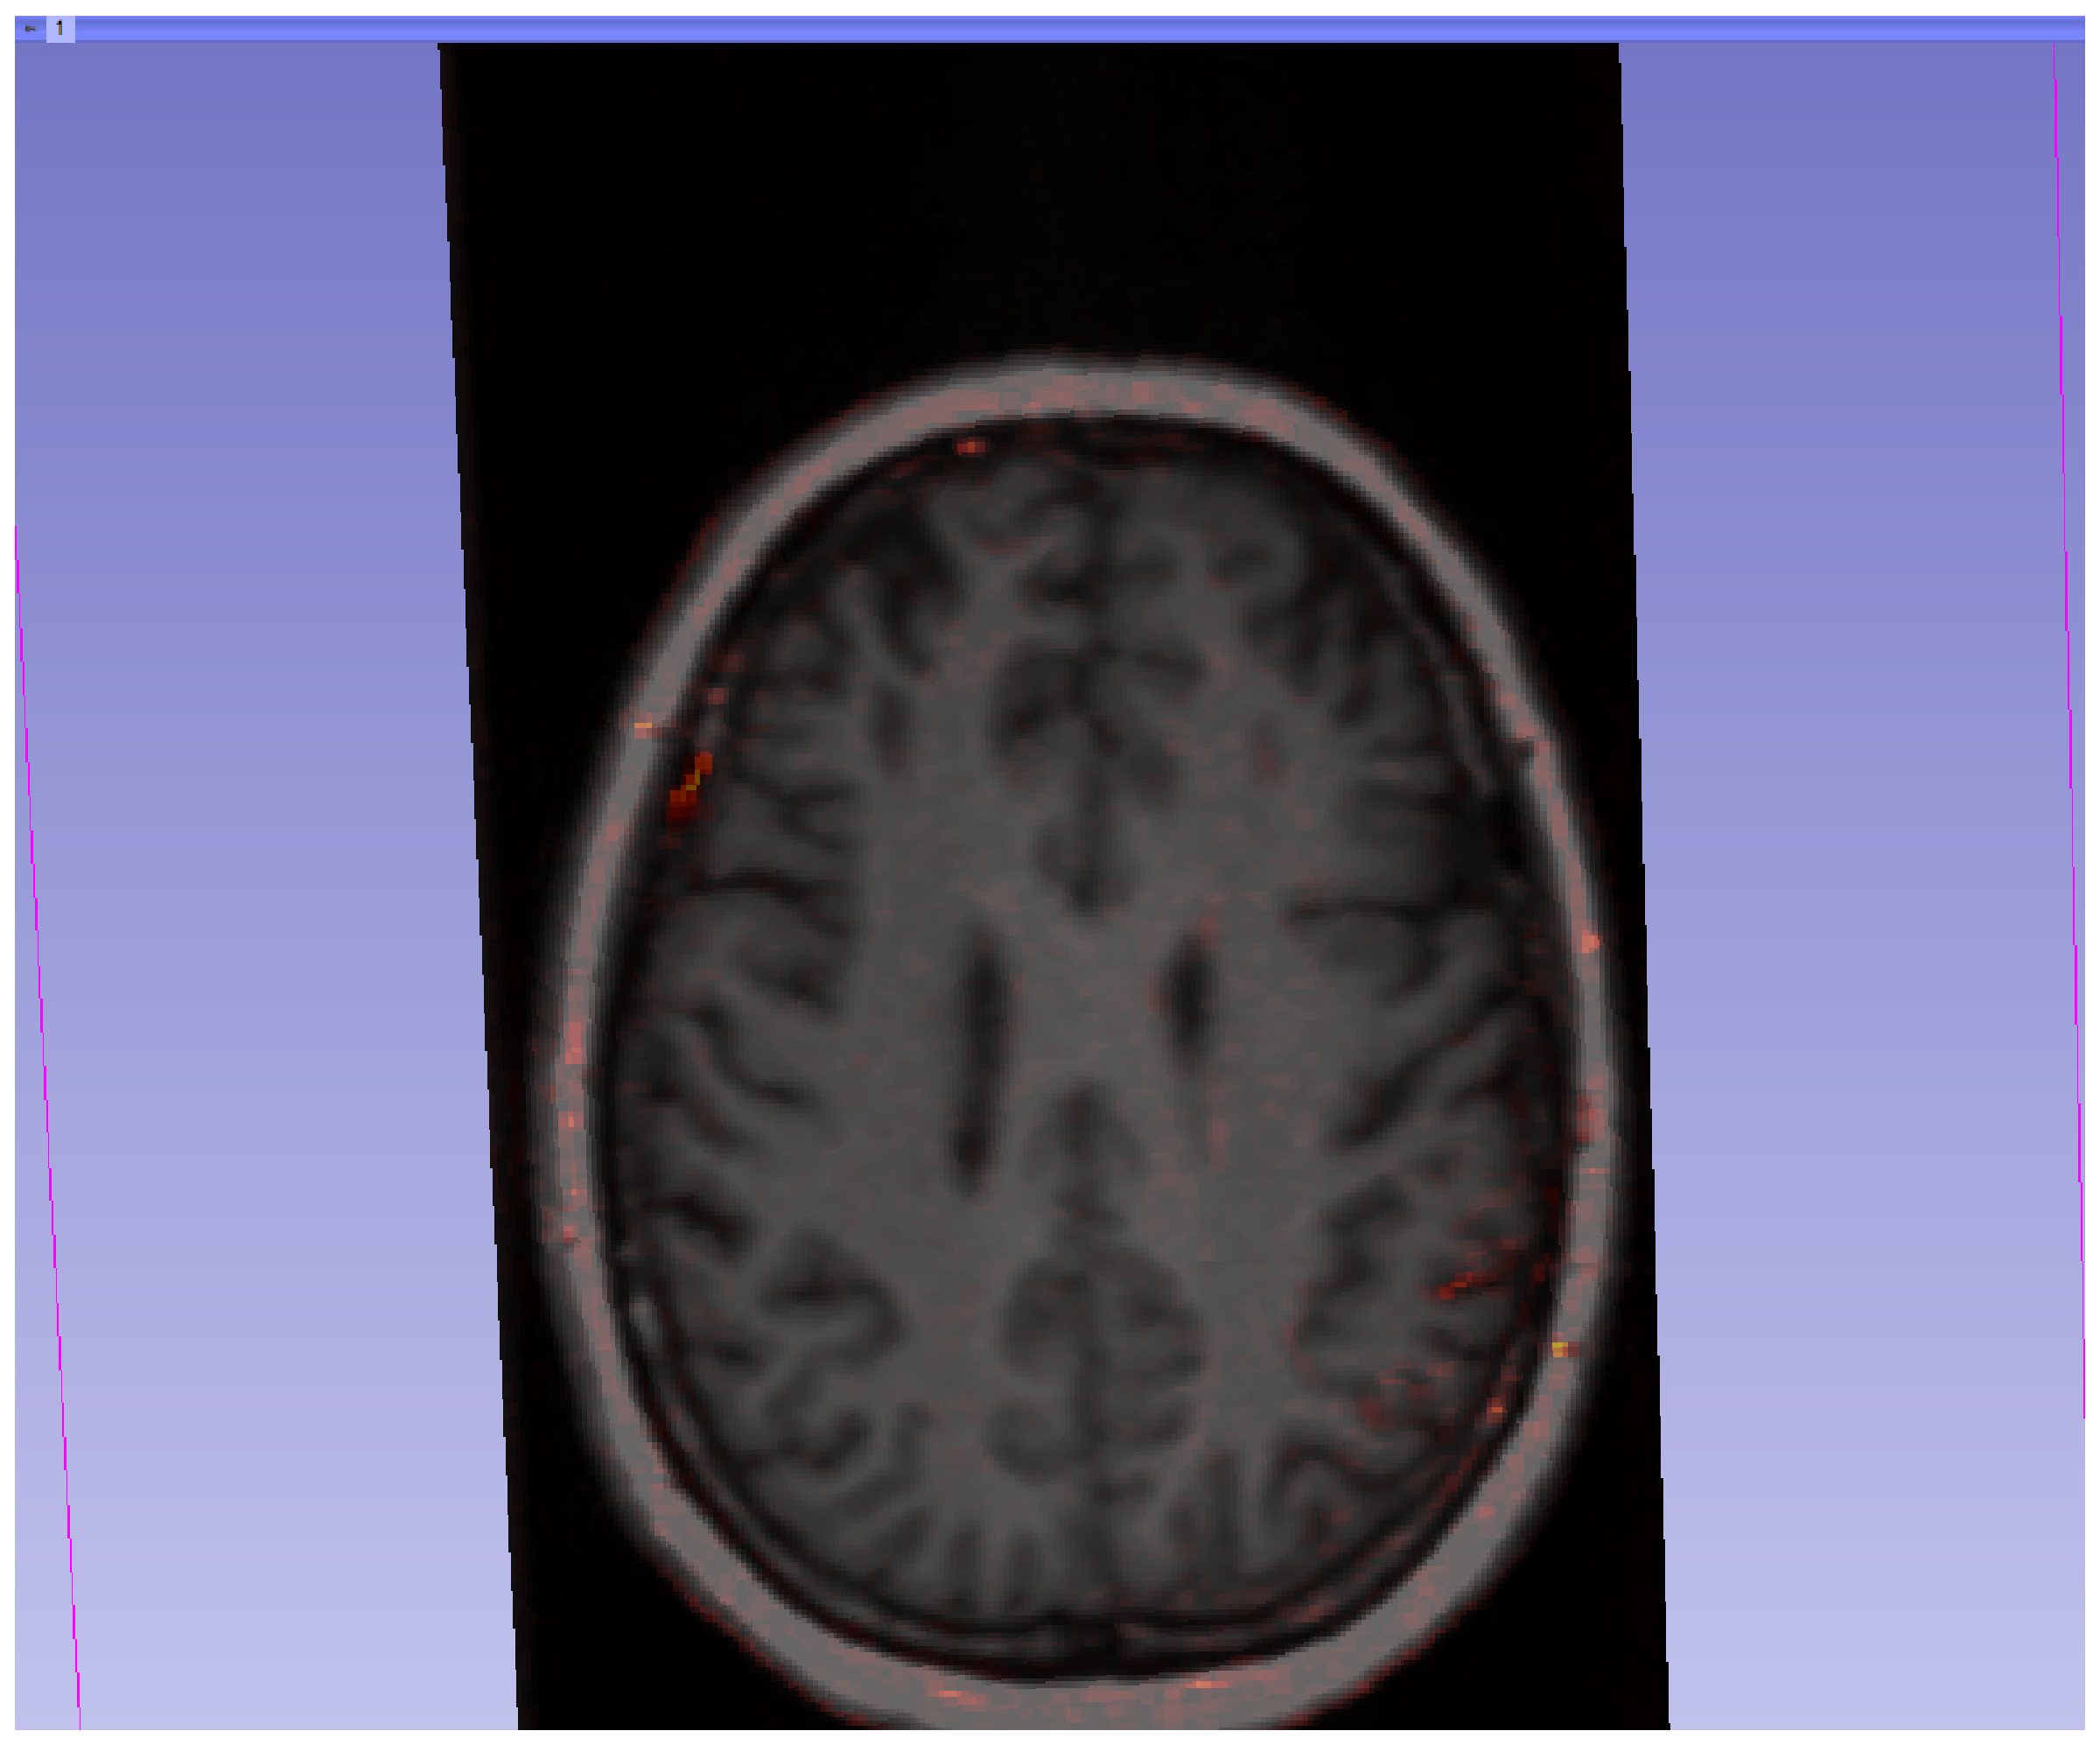
\includegraphics[scale=0.2]{/experiment_CL_P1/CL_Traversal.eps}
  \caption{Voxel-based method. Patient 1: Traversal plane}
  \label{CL_Traversal}
\end{figure}

\begin{figure}[H]
  \centering
  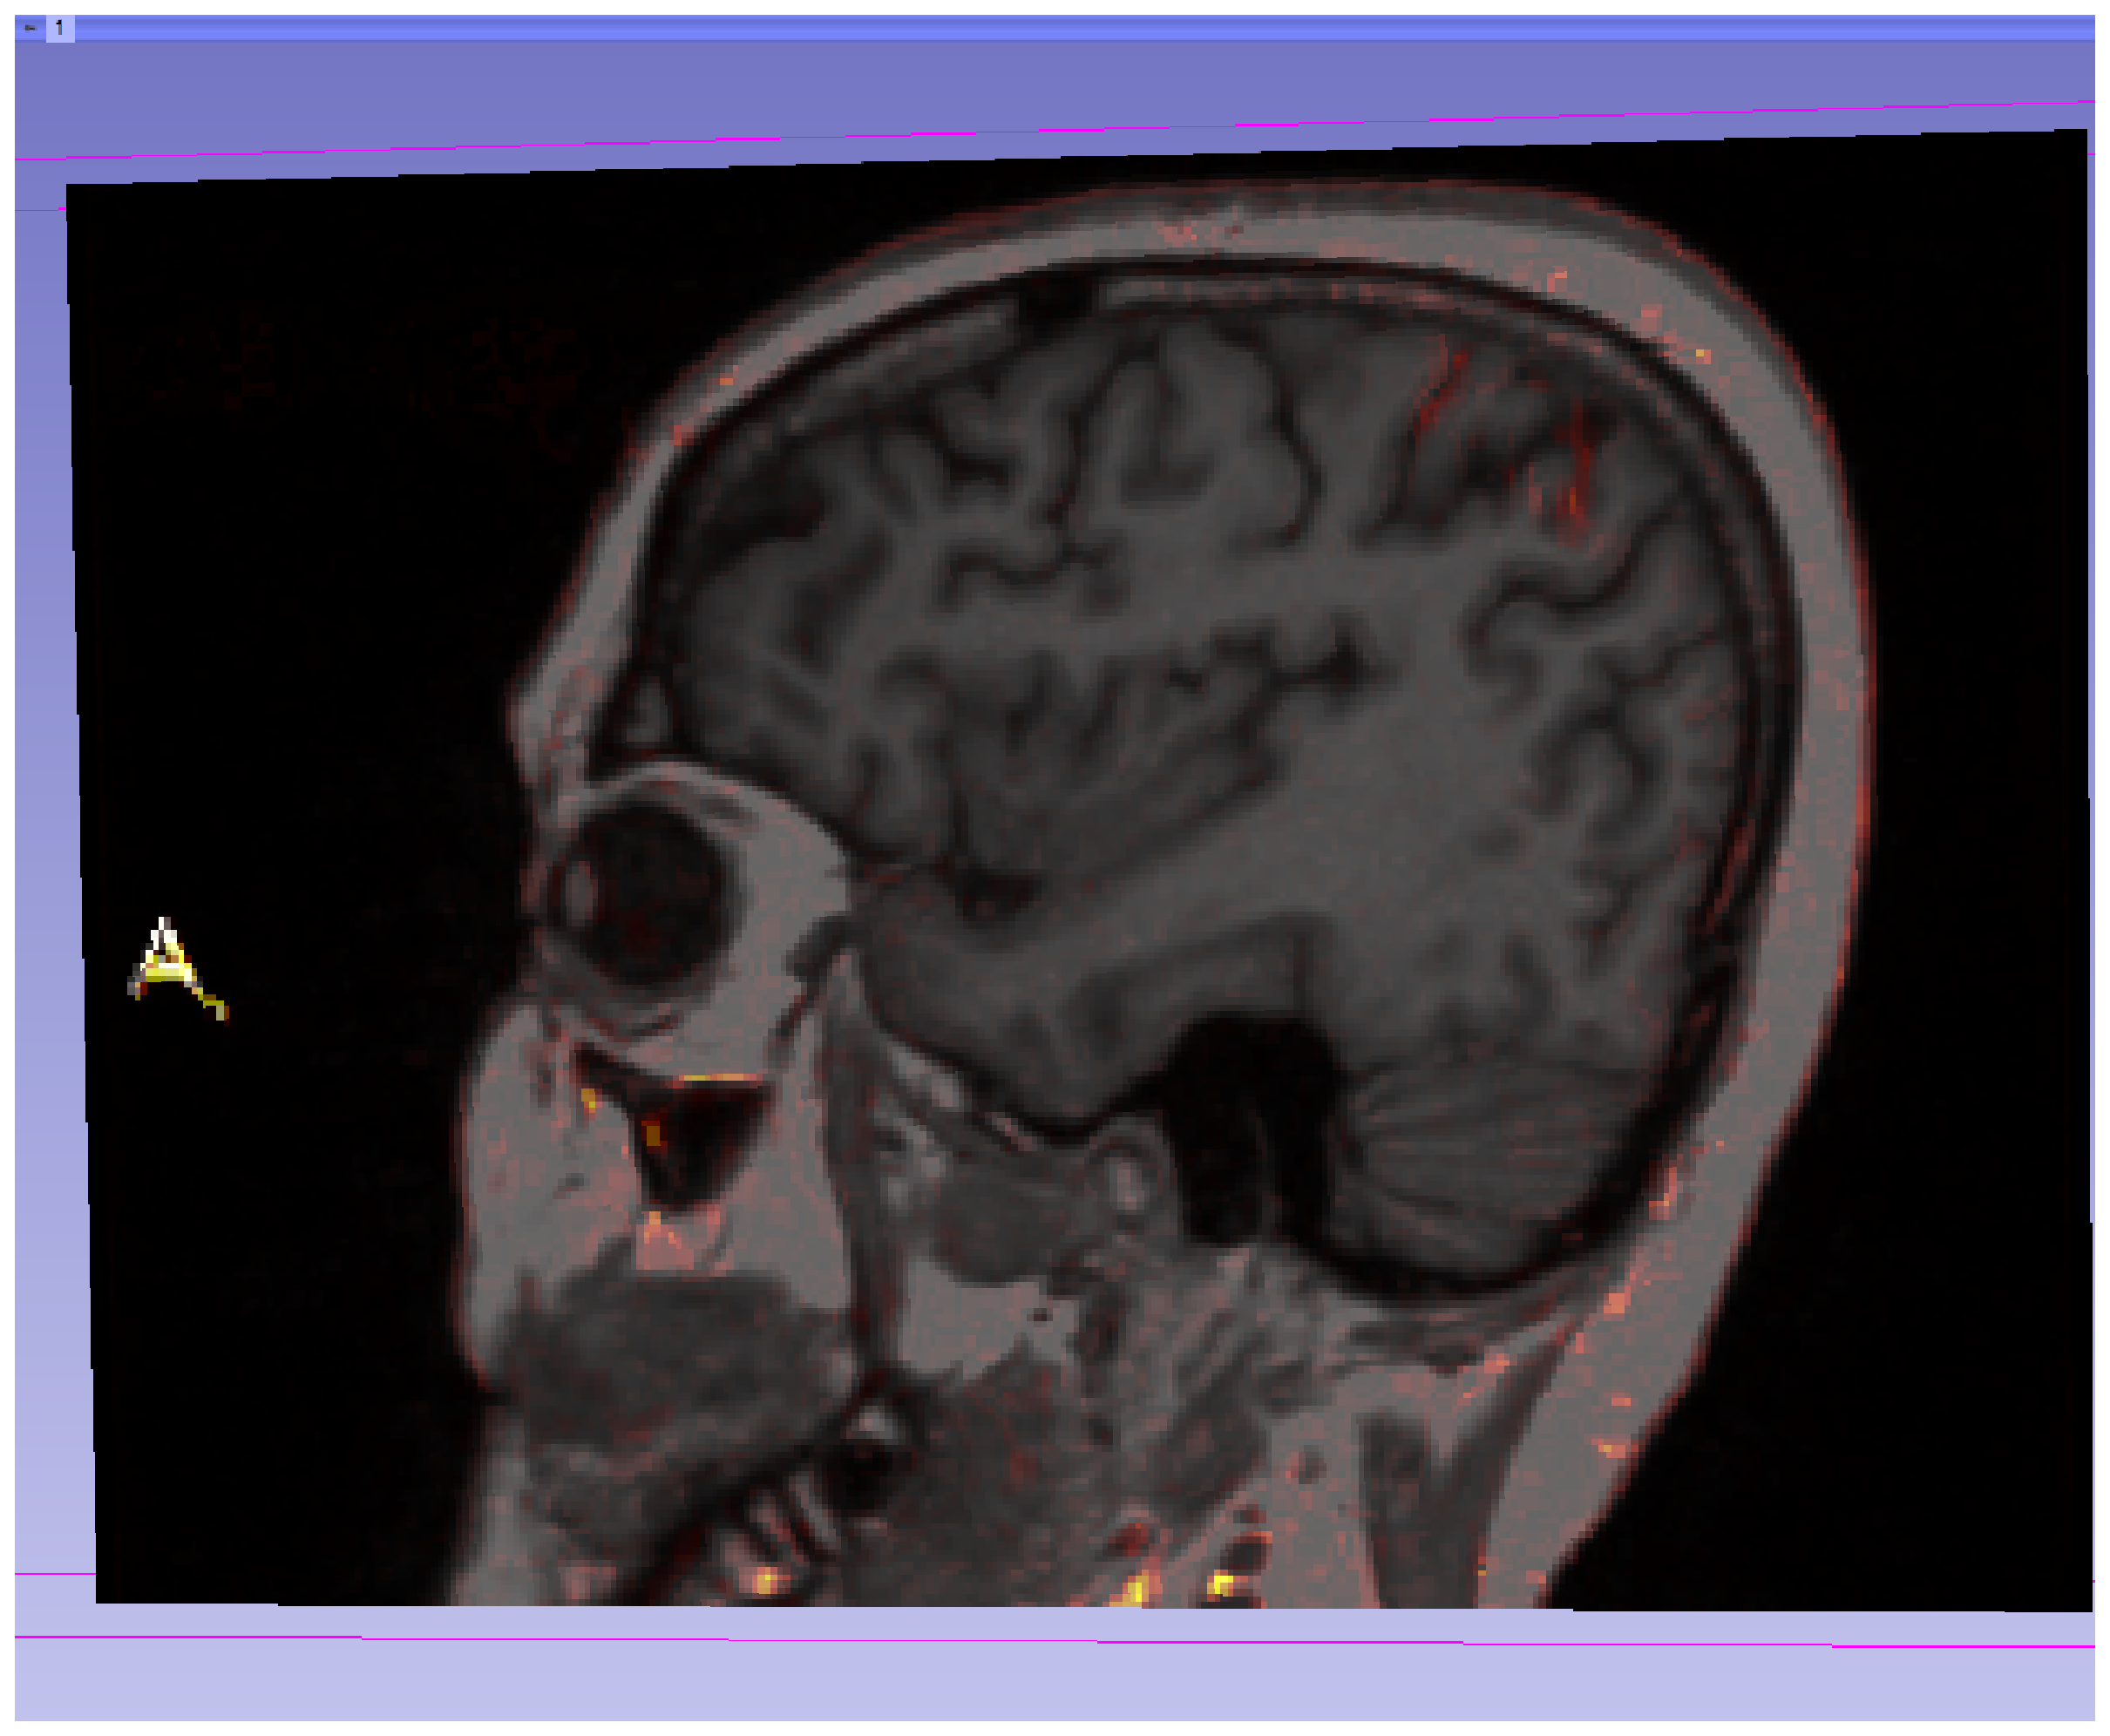
\includegraphics[scale=0.2]{/experiment_CL_P1/CL_Sagittal.eps}
  \caption{Voxel-based method. Patient 1: Sagittal plane}
  \label{CL_Sagittal}
\end{figure}


\subsubsection{Tensor-based Method}
Parameters used:
\begin{description}
\item \textit{Deformation field smoothing sigma:} 2.5
\item \textit{Shrinkage percentage:} 70
\item \textit{Growth percentage:} 75
\end{description}

\begin{figure}[H]
  \centering
  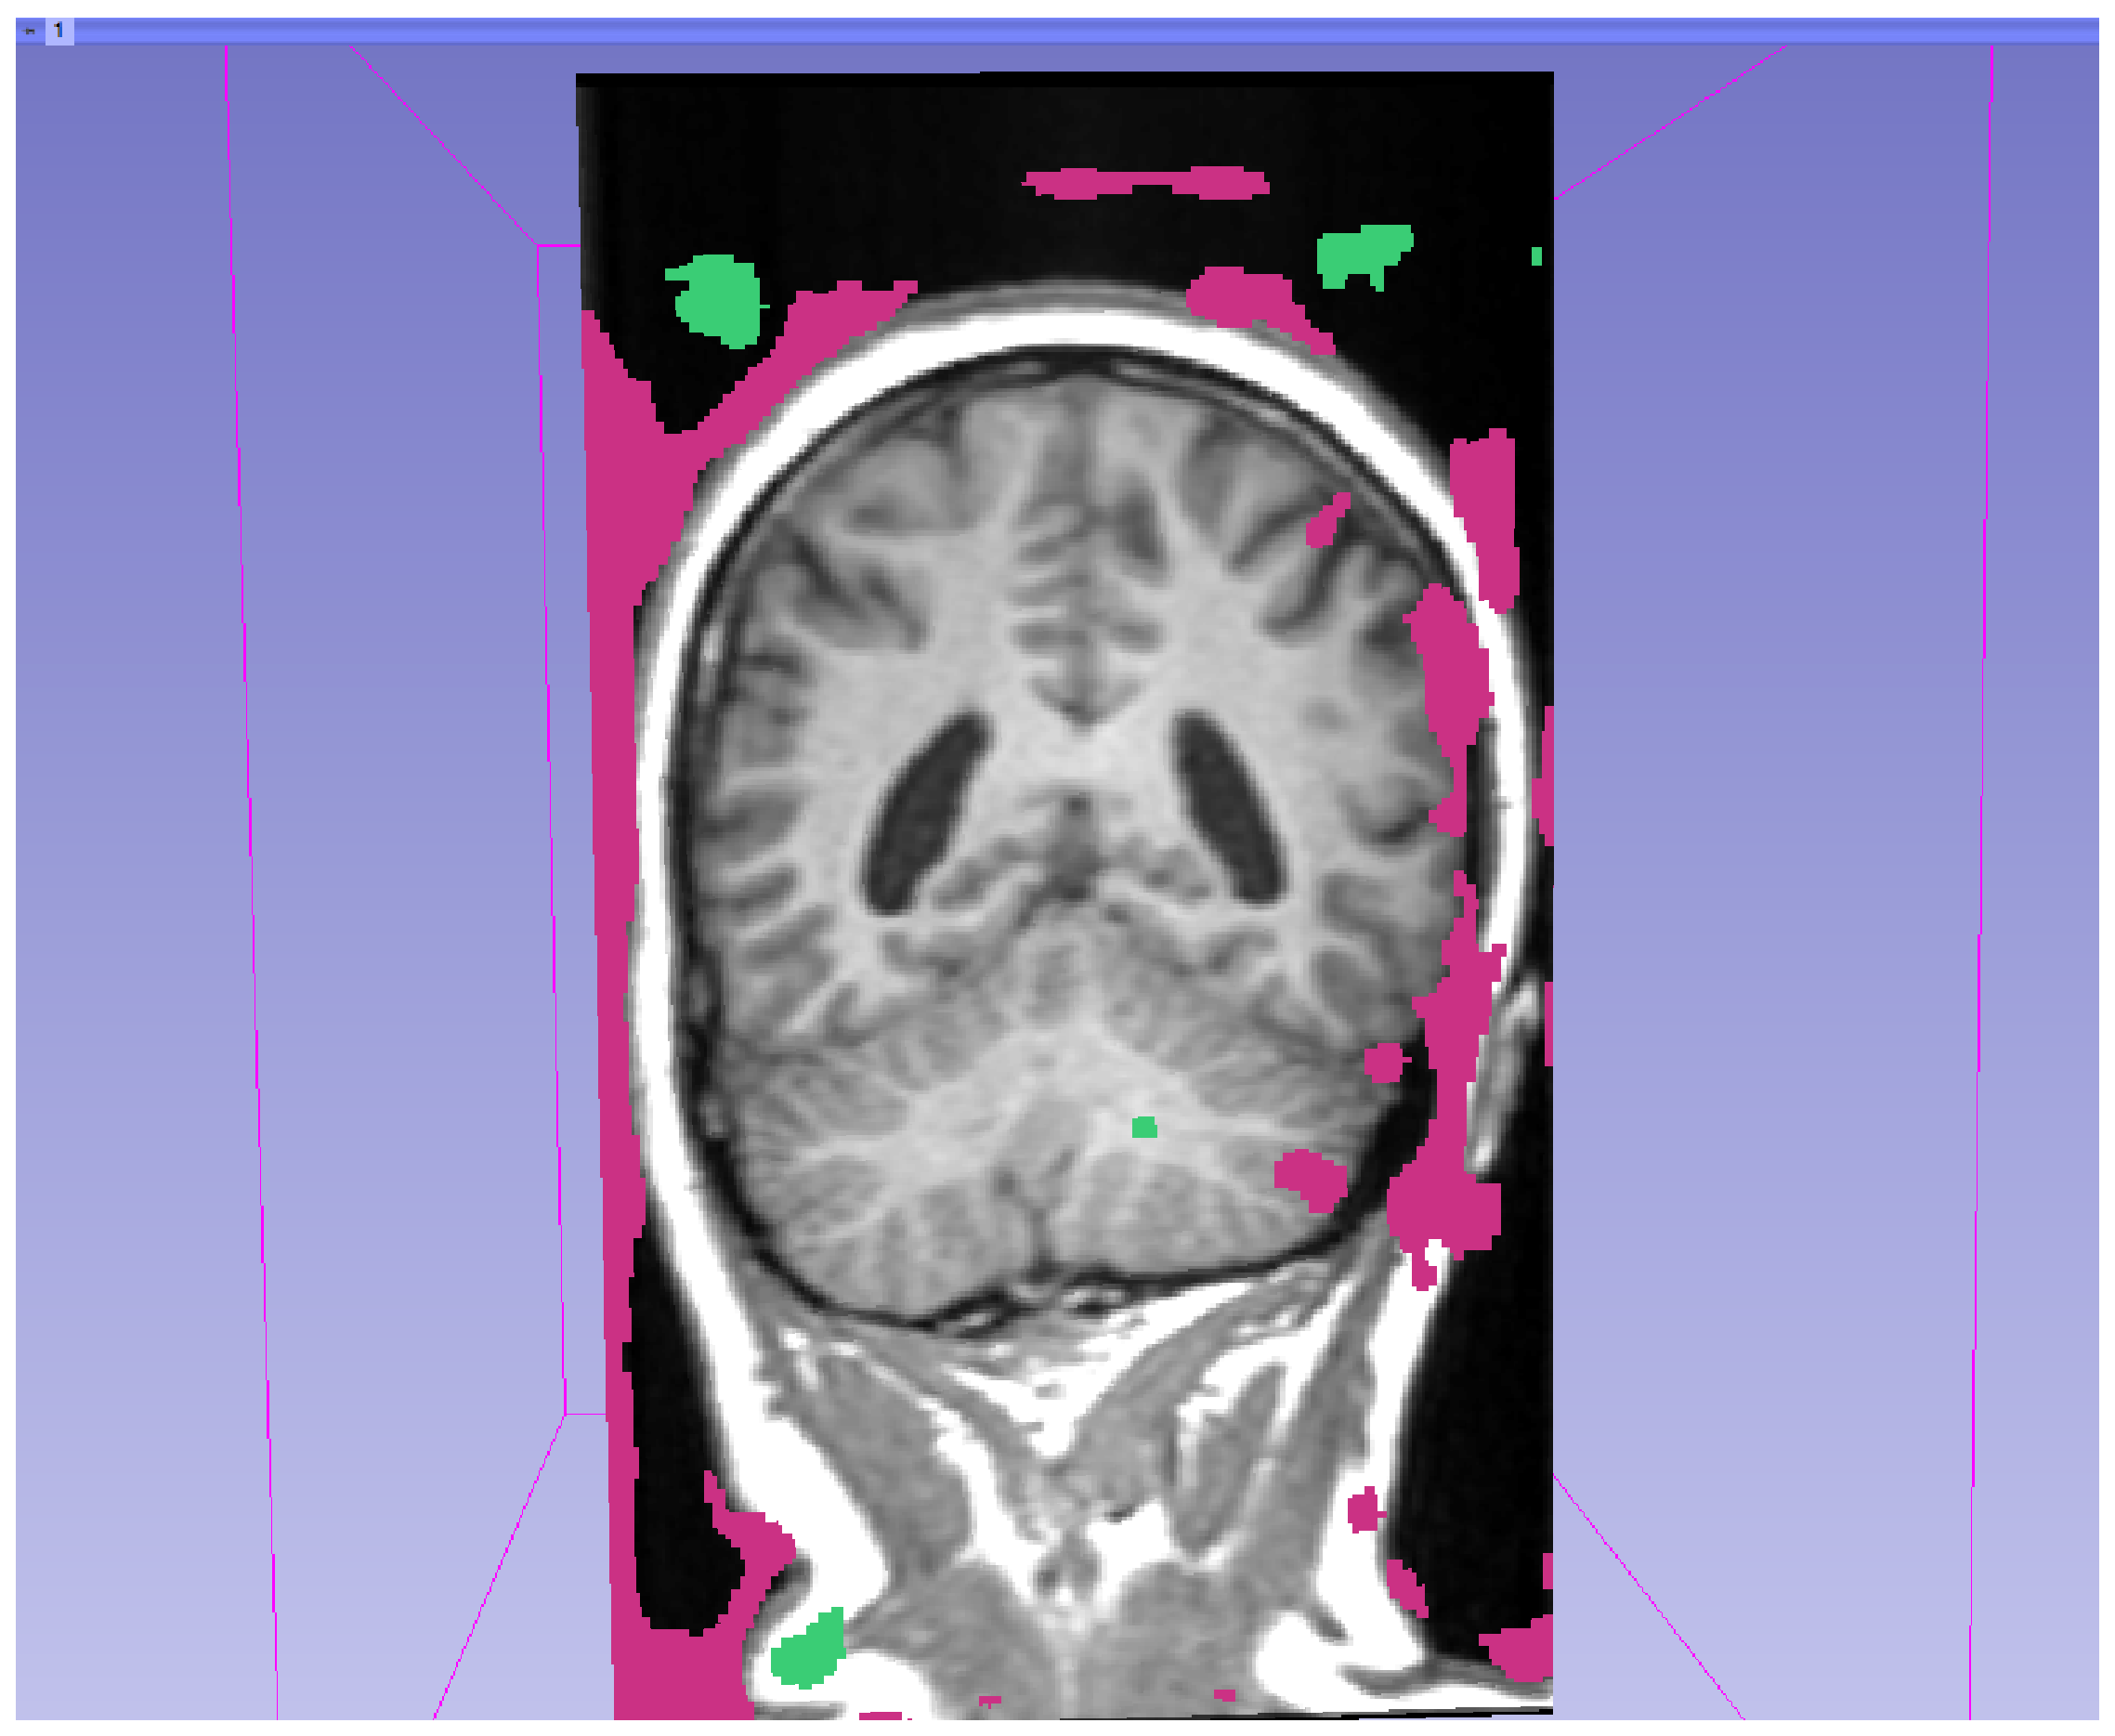
\includegraphics[scale=0.2]{/experiment_CL_P1/CL_Tensor_Coronal.eps}
  \caption{Tensor-based method. Patient 1: Coronal plane}
  \label{CL_TCoronal}
\end{figure}

\begin{figure}[H]
  \centering
  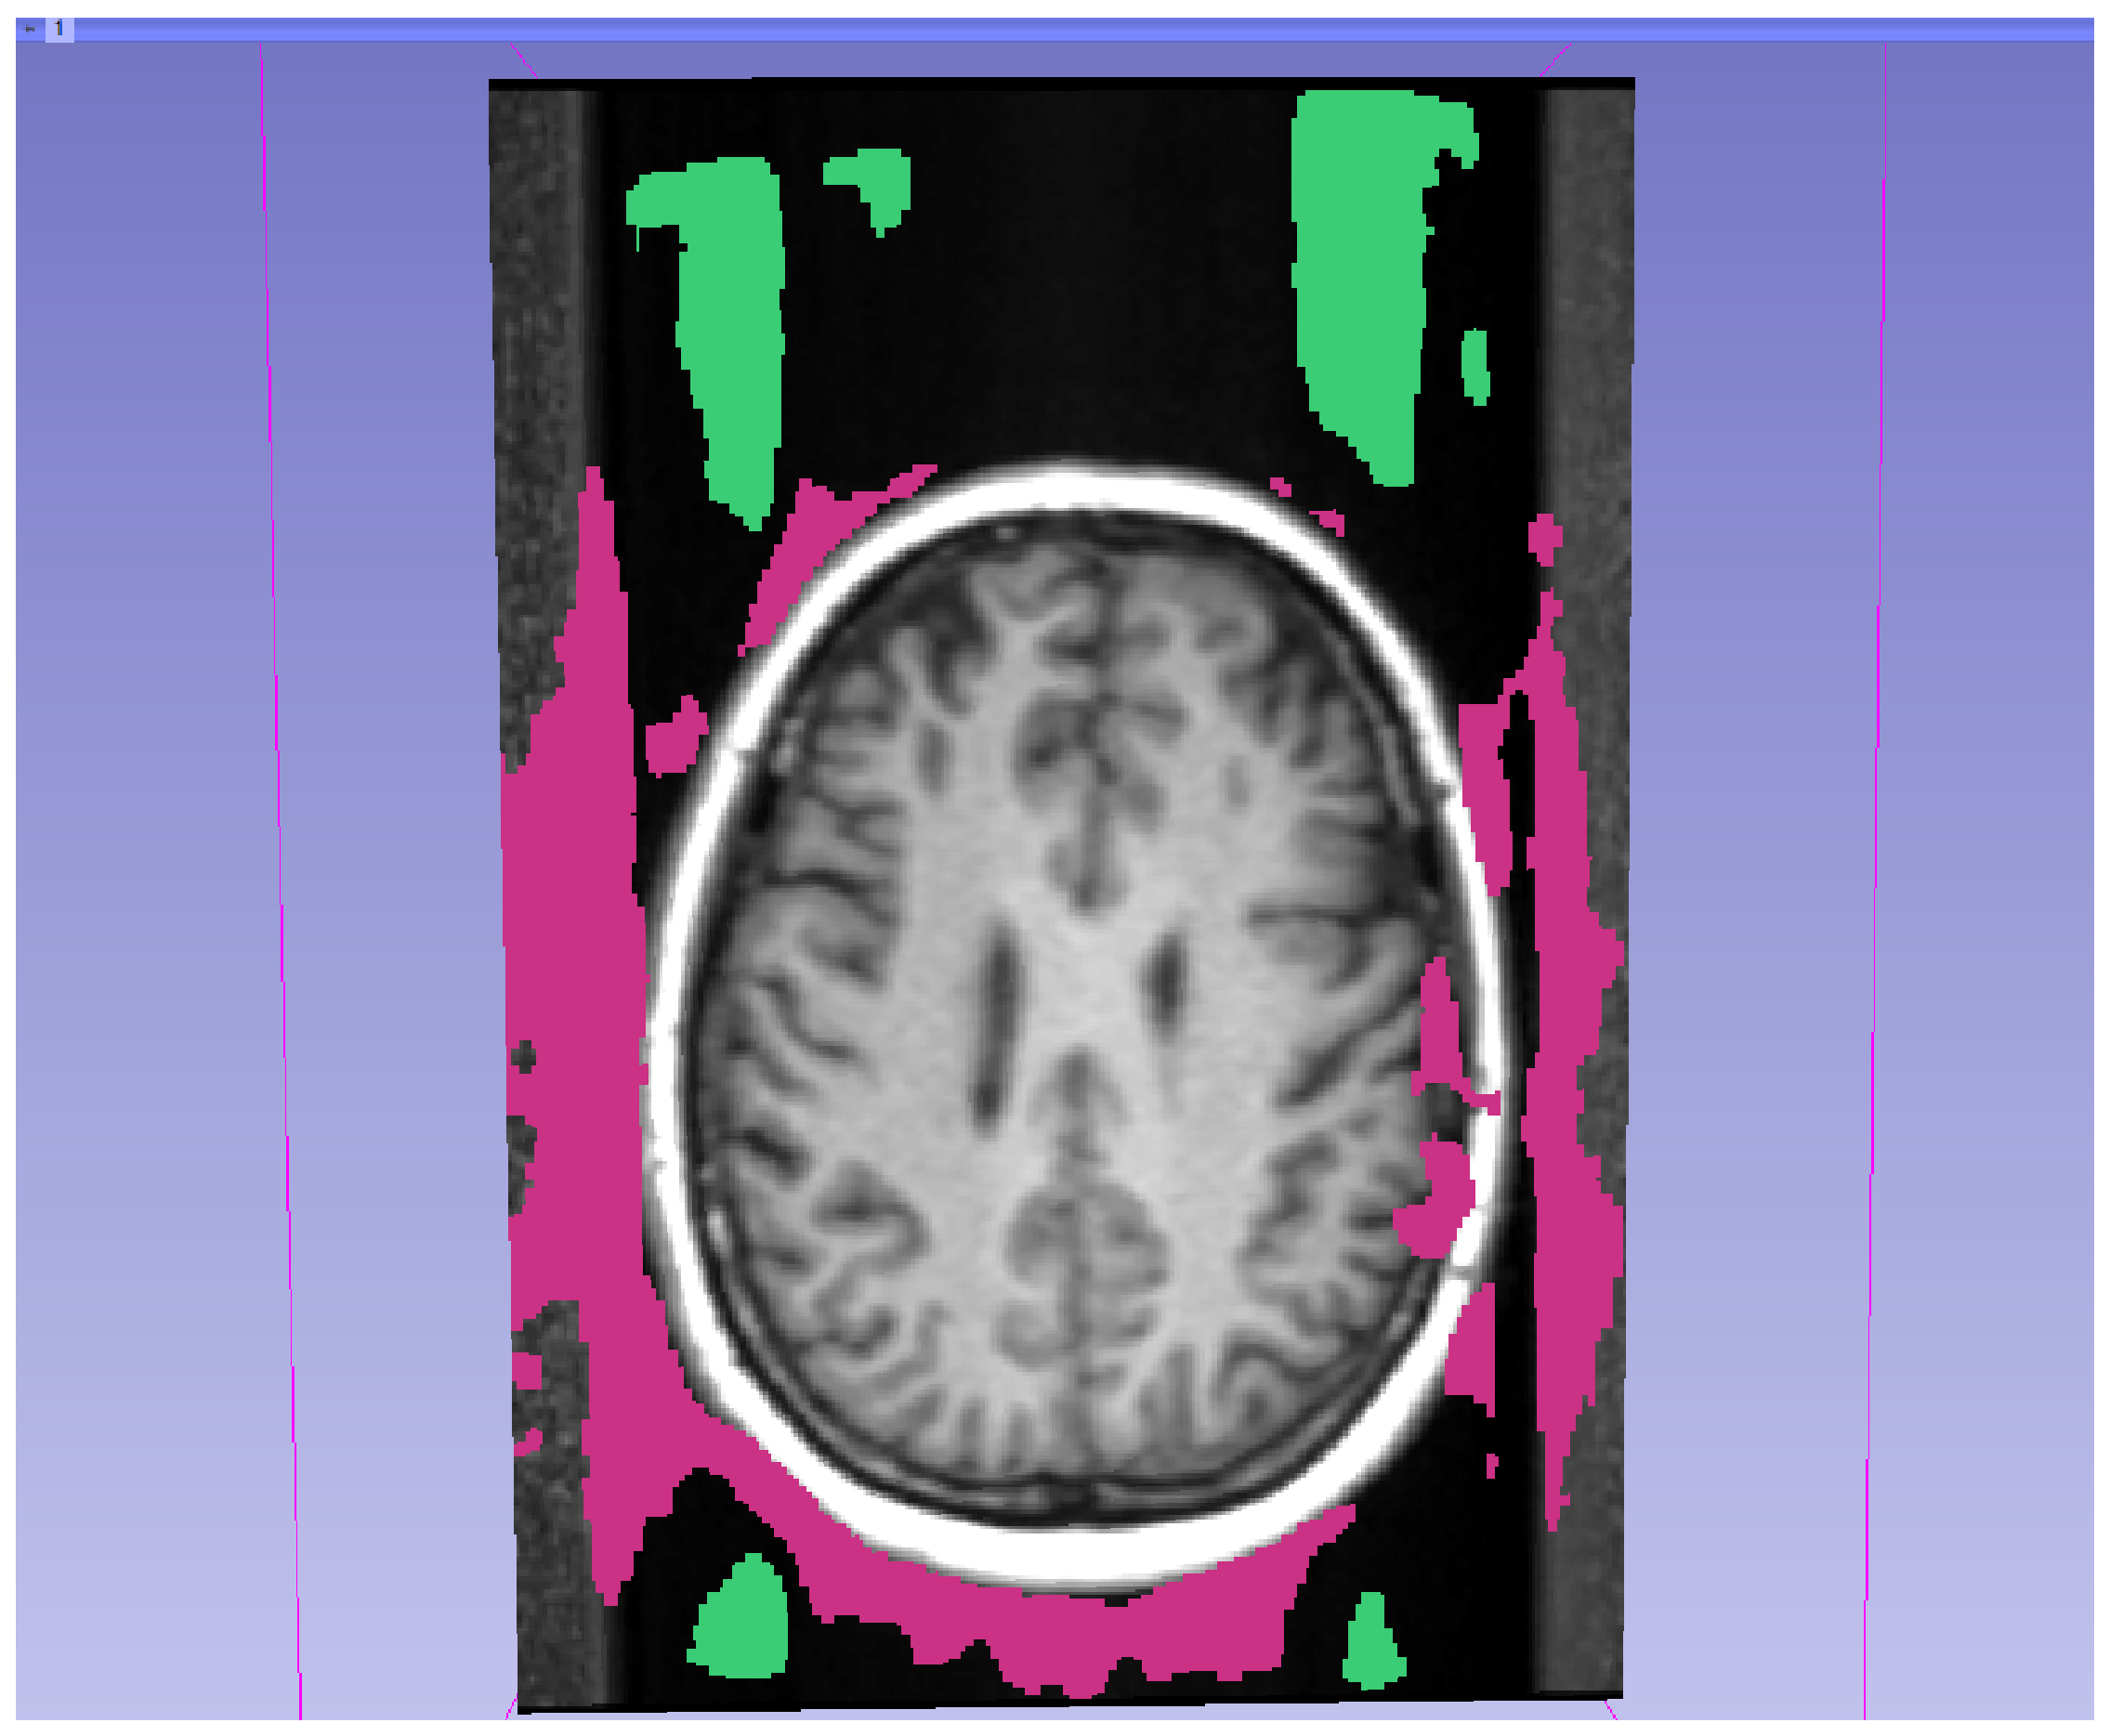
\includegraphics[scale=0.2]{/experiment_CL_P1/CL_Tensor_Traversal.eps}
  \caption{Tensor-based method. Patient 1: Traversal plane}
  \label{CL_TTraversal}
\end{figure}

\begin{figure}[H]
  \centering
  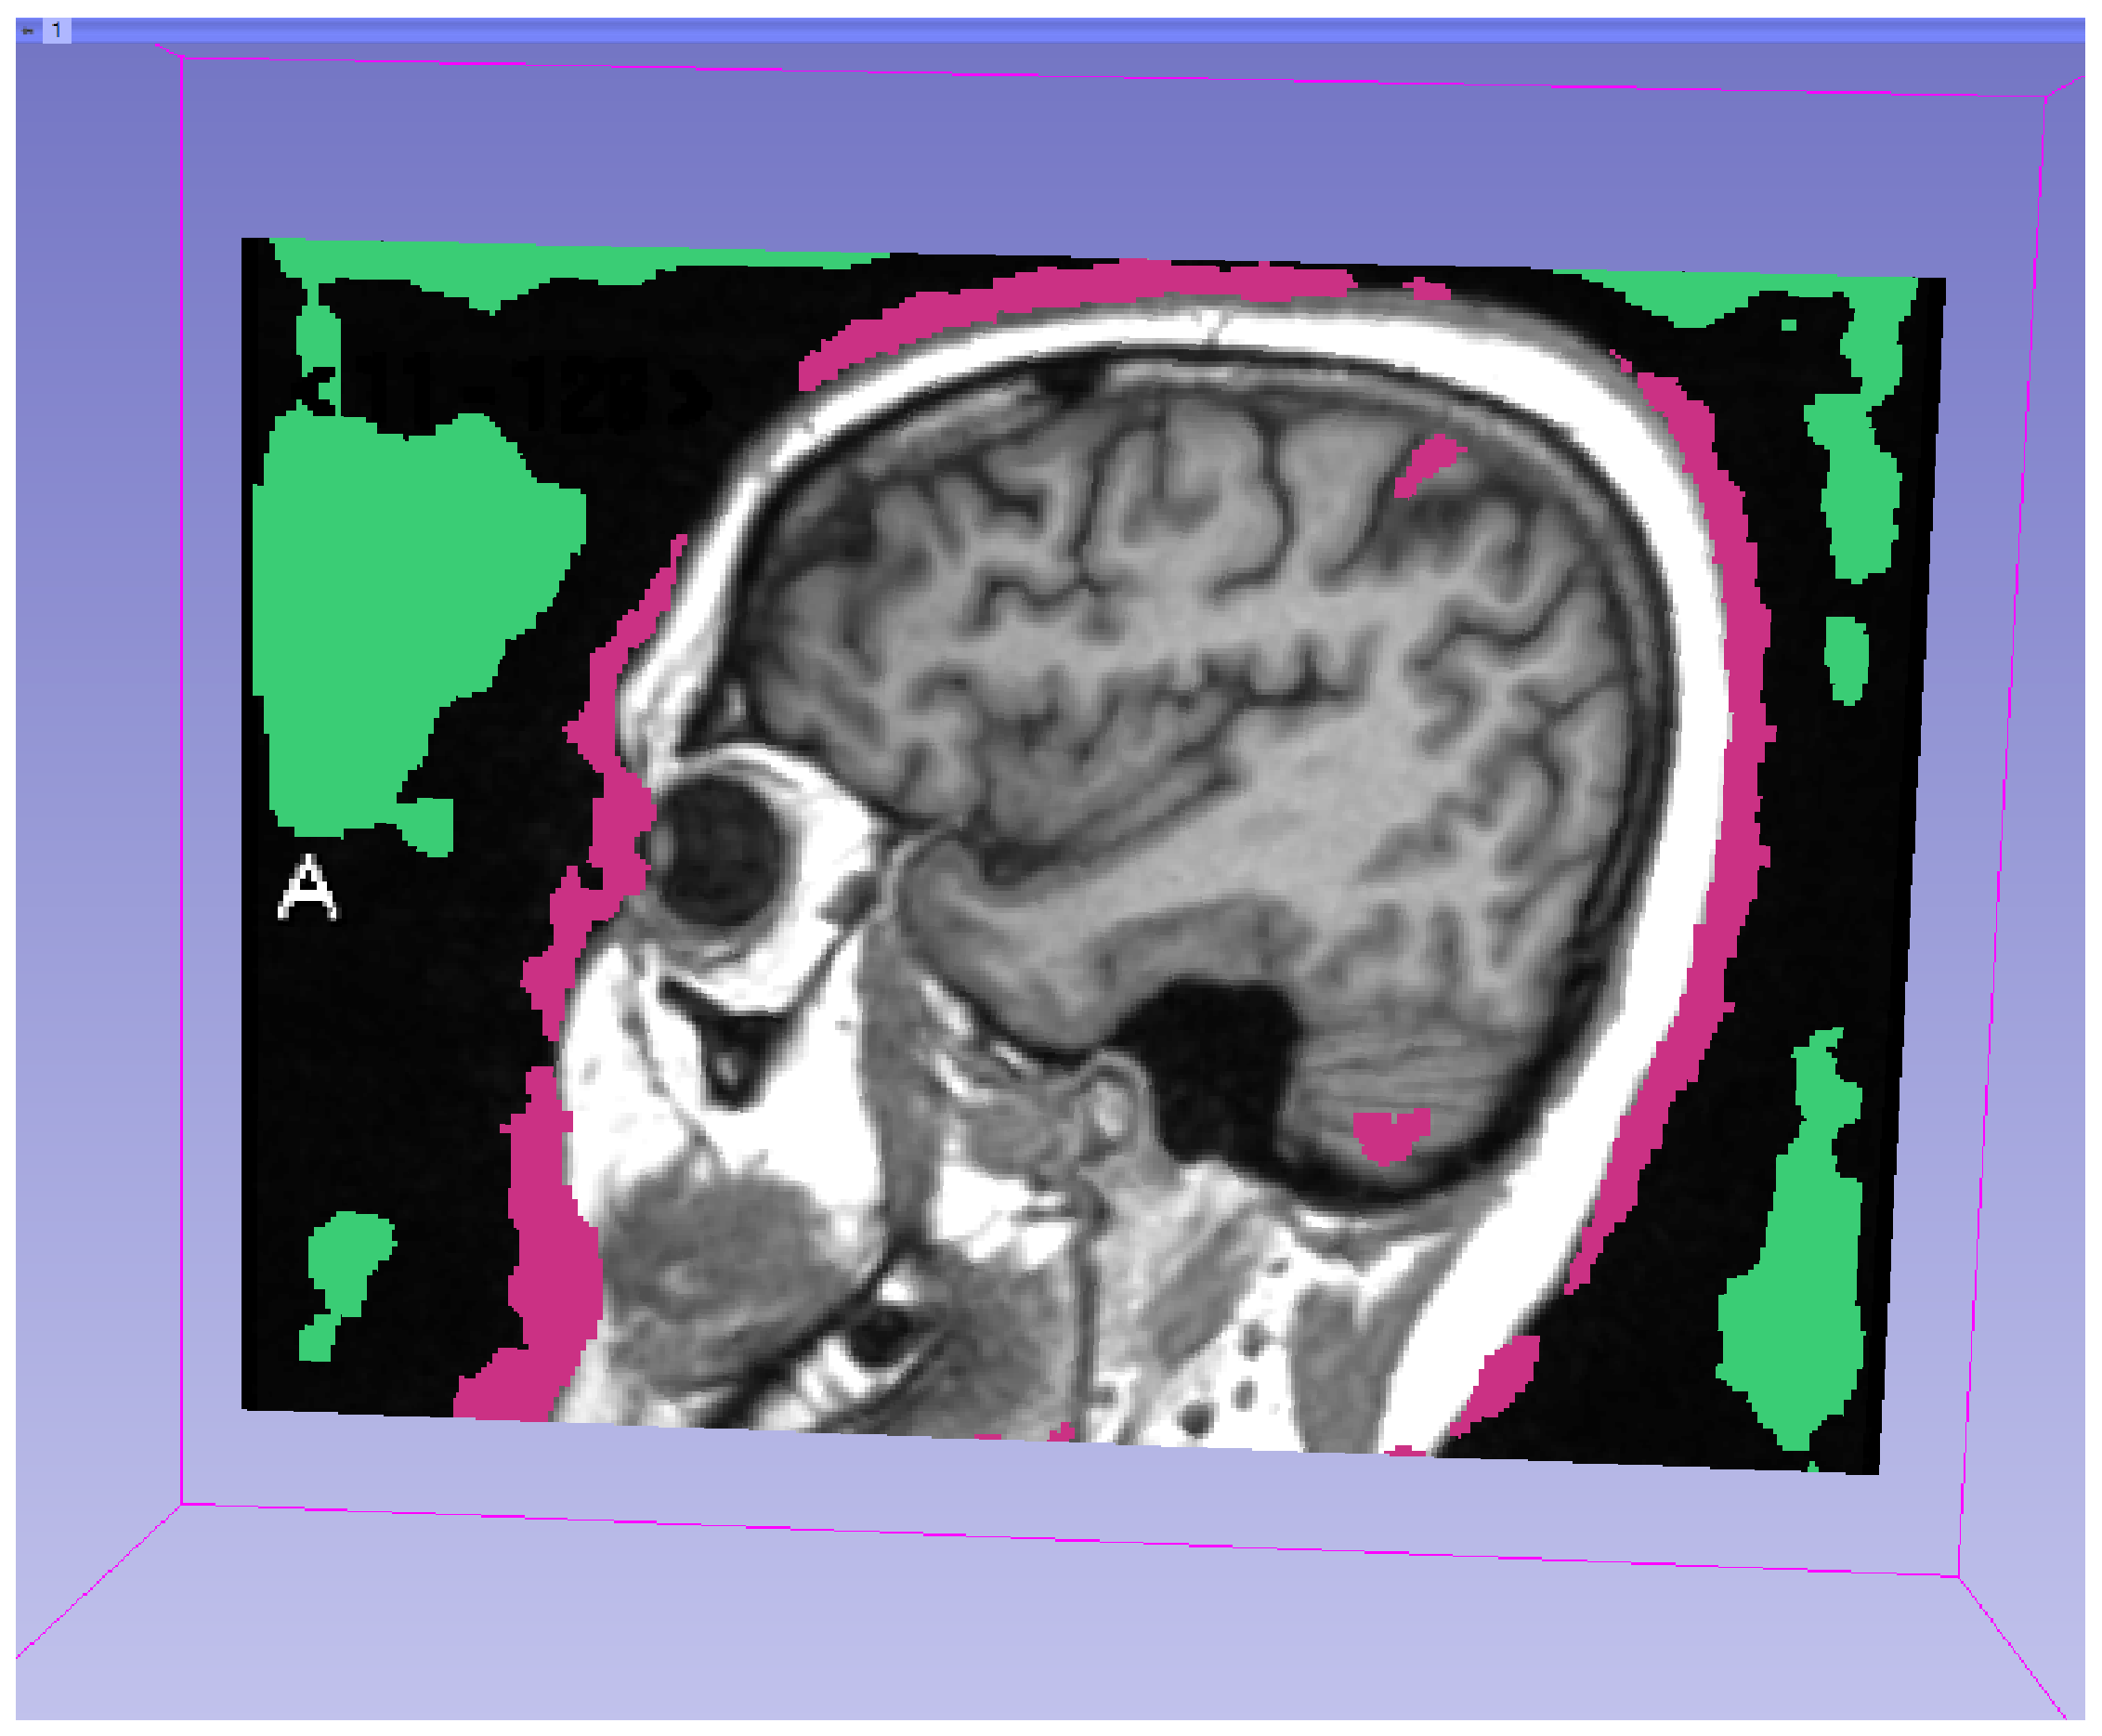
\includegraphics[scale=0.2]{/experiment_CL_P1/CL_Tensor_Sagittal.eps}
  \caption{Tensor-based method. Patient 1: Sagittal plane}
  \label{CL_TSagittal}
\end{figure}


\subsection{Patient 2}
The differences in this patient, if actually present, are really
small. 

\subsubsection{Voxel-based Method}
The voxel-based method shows small differences near the corpus
callosum on the three planes; this differences, accourding to the
medical expert, might be real because this is a very common area
affected by trauma.\\

The registration method used was \textit{Affine registration}.

\begin{figure}[H]
  \centering
  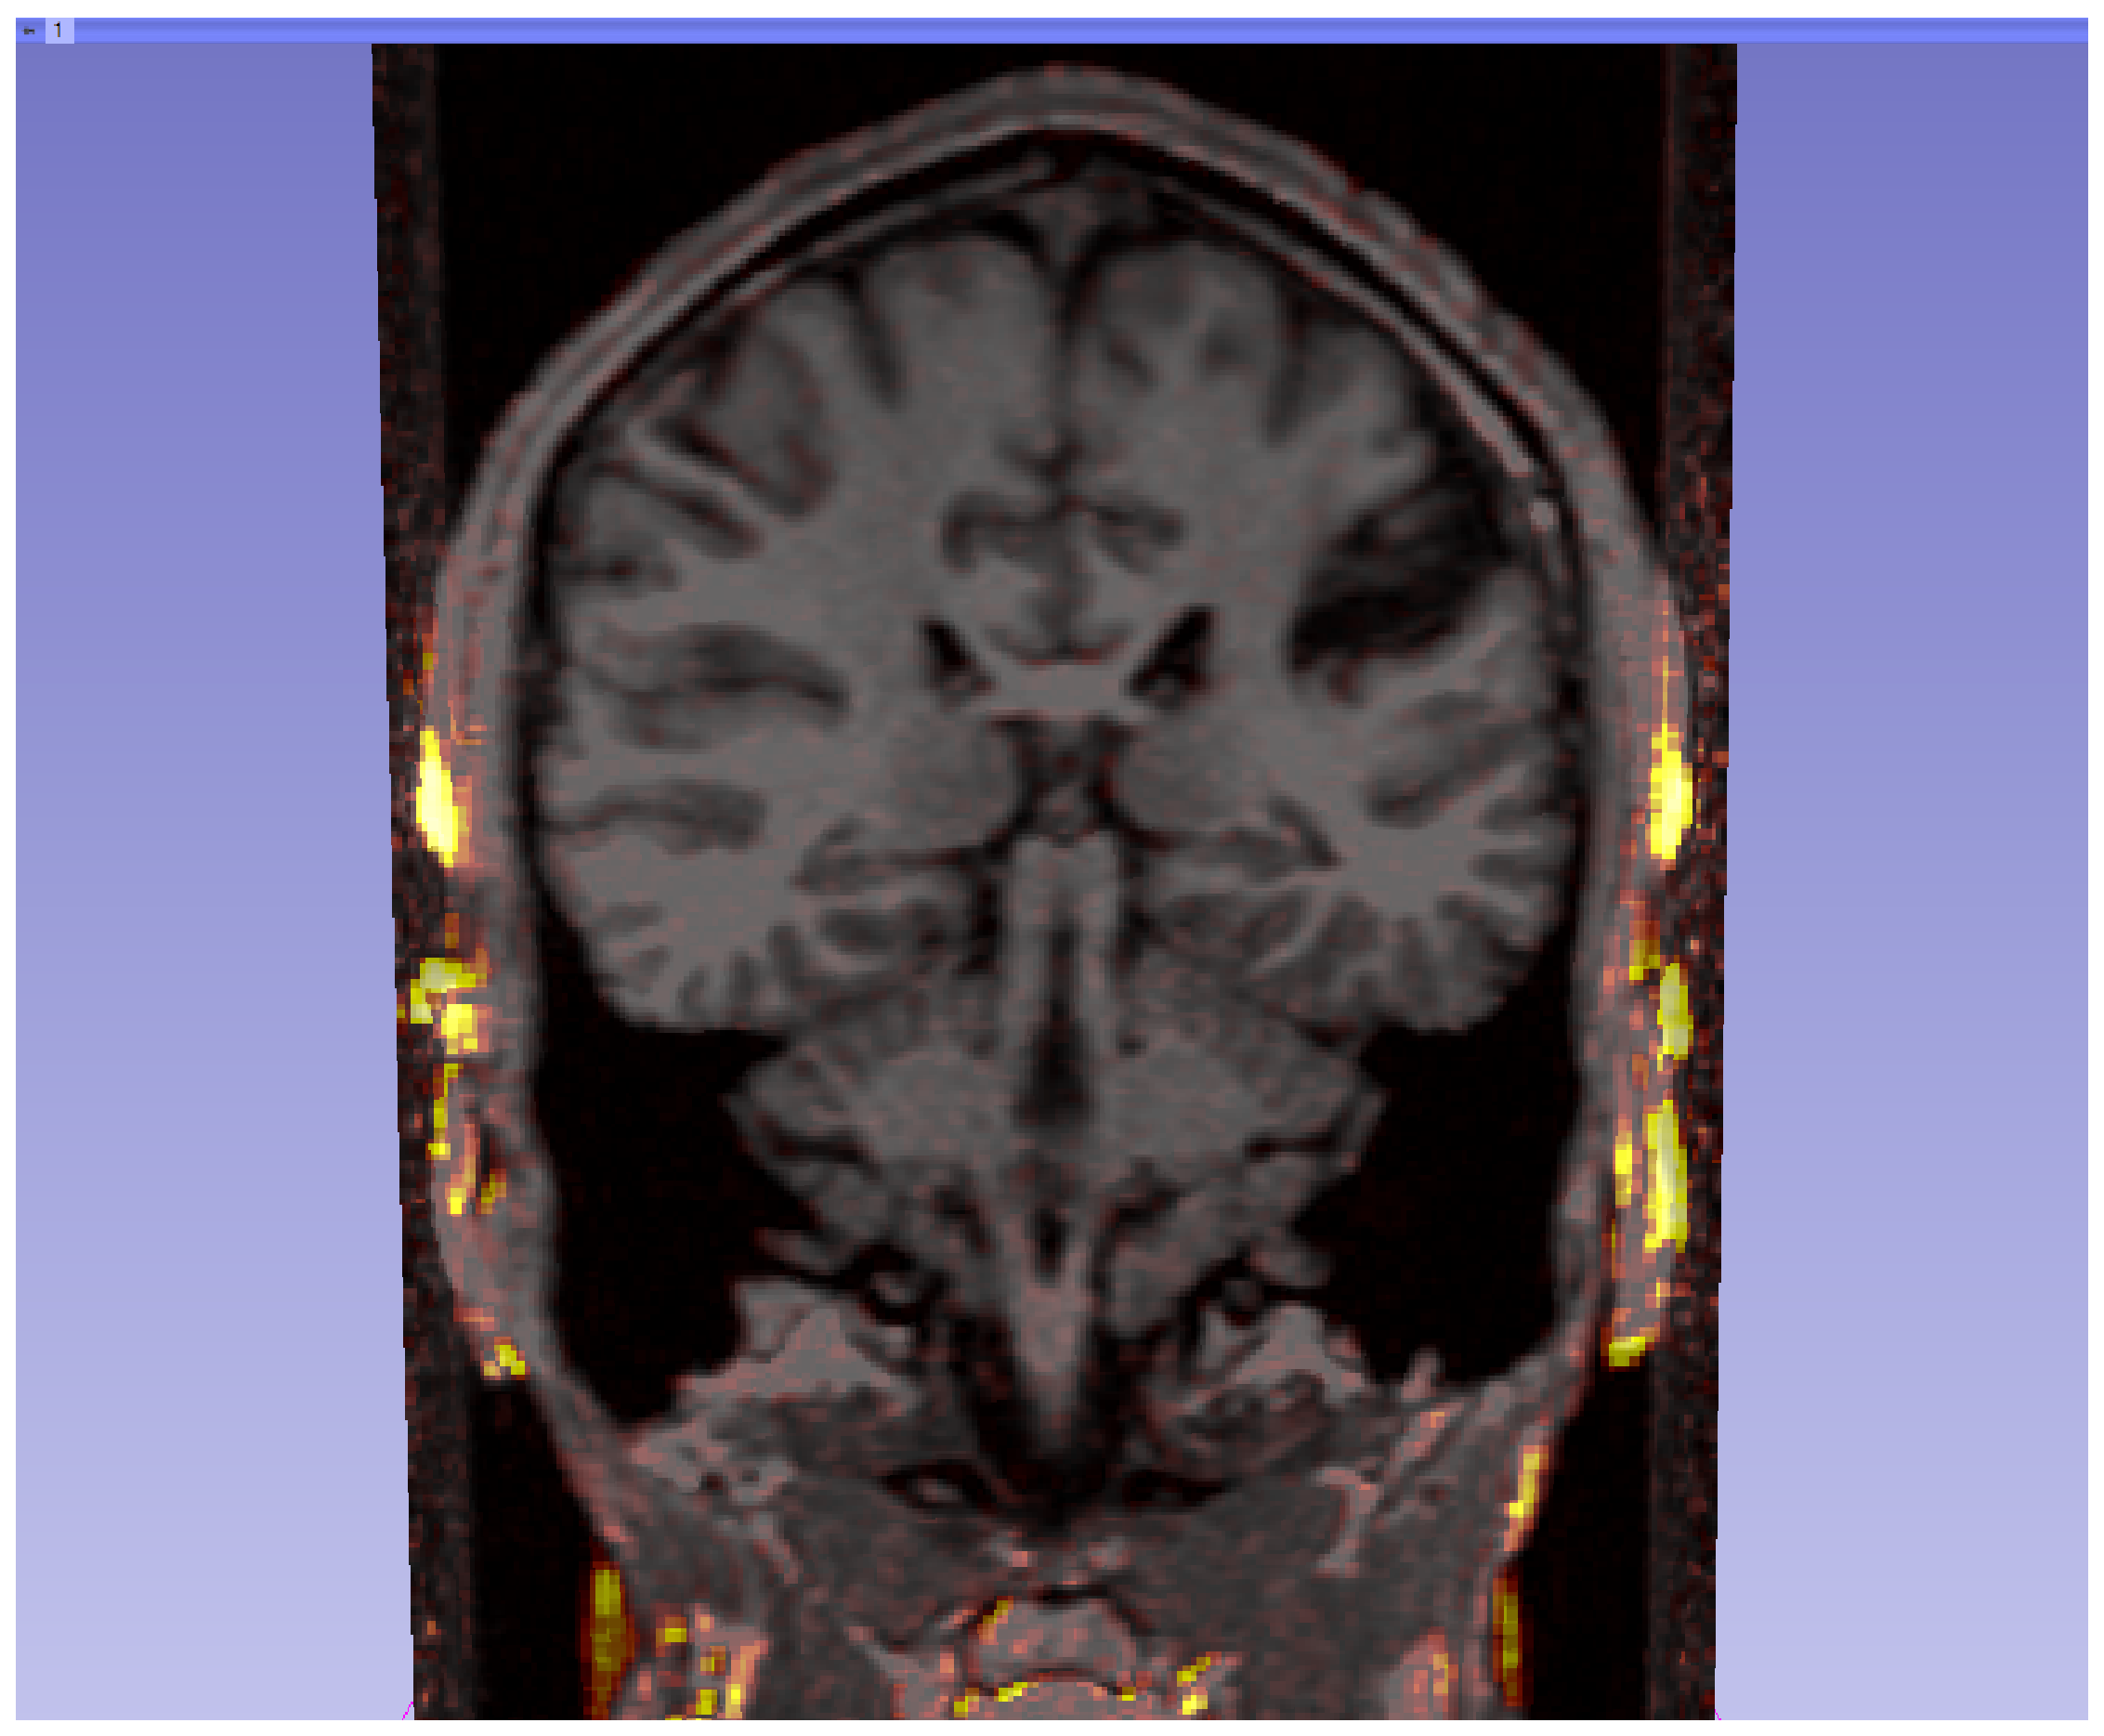
\includegraphics[scale=0.2]{/experiment_PB_P2/PB_Coronal.eps}
  \caption{Voxel-based method. Patient 2: Coronal plane}
  \label{PB_Coronal}
\end{figure}

\begin{figure}[H]
  \centering
  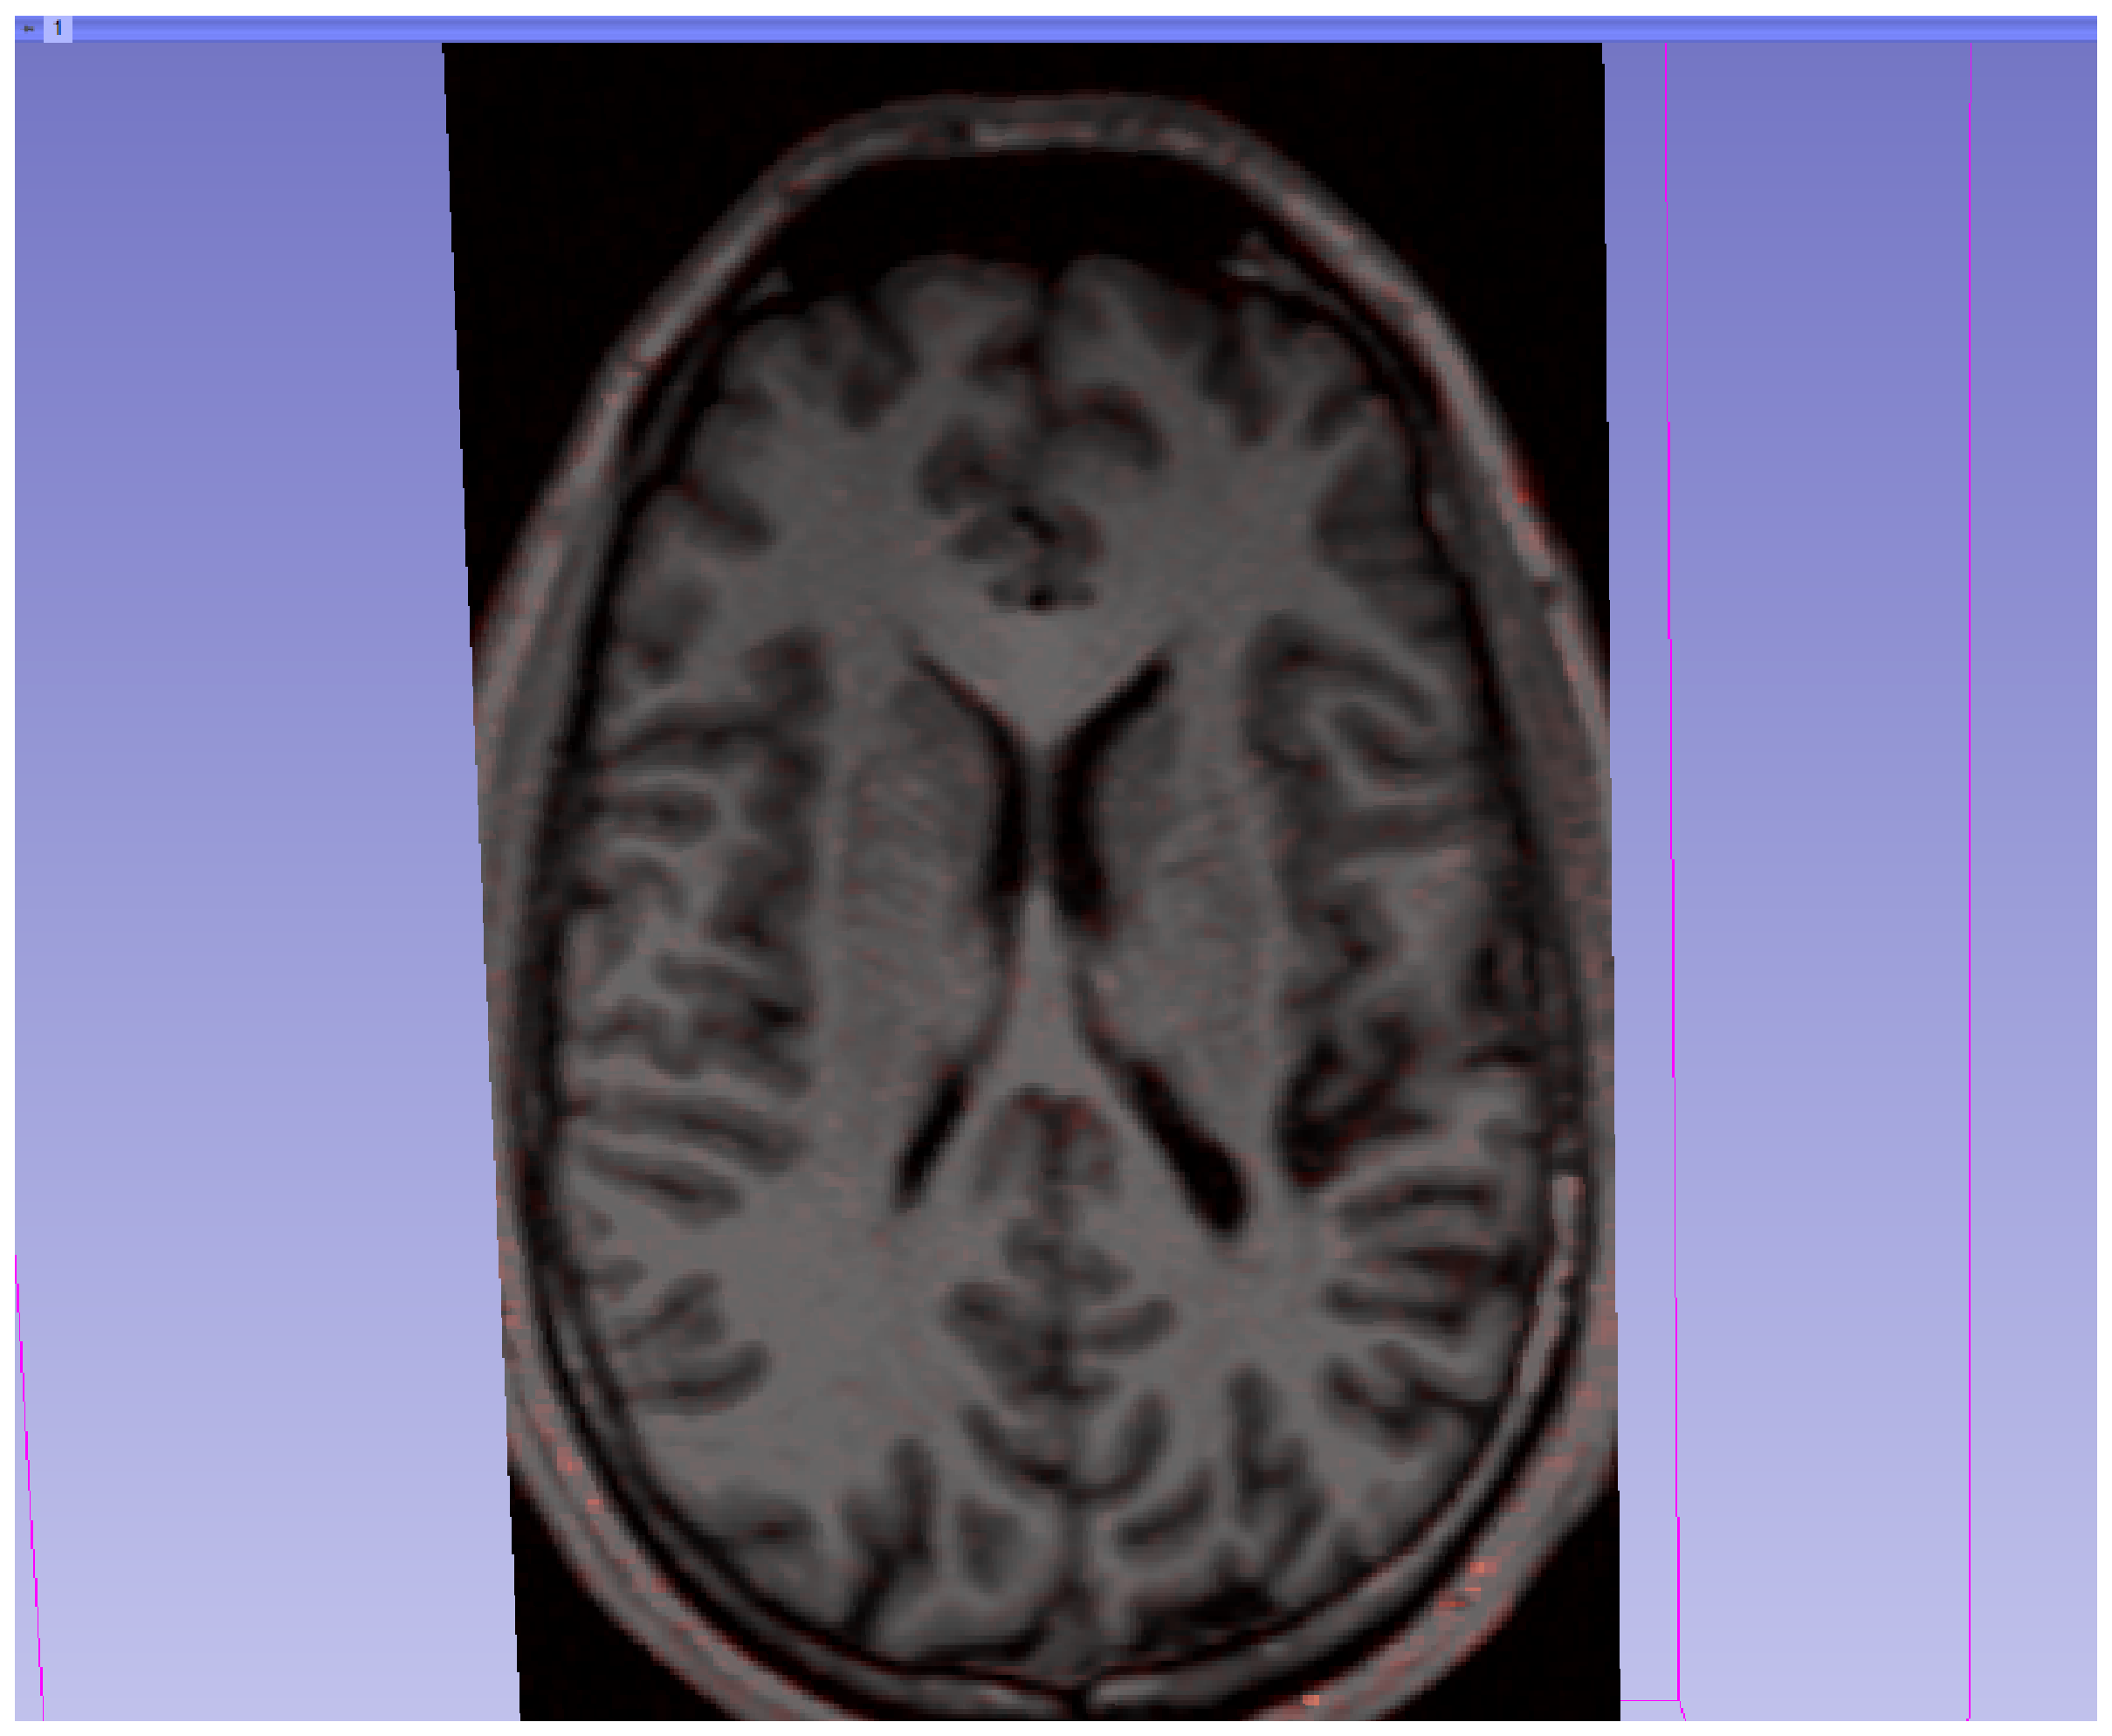
\includegraphics[scale=0.2]{/experiment_PB_P2/PB_Traversal.eps}
  \caption{Voxel-based method. Patient 2: Traversal plane}
  \label{PB_Traversal}
\end{figure}

\begin{figure}[H]
  \centering
  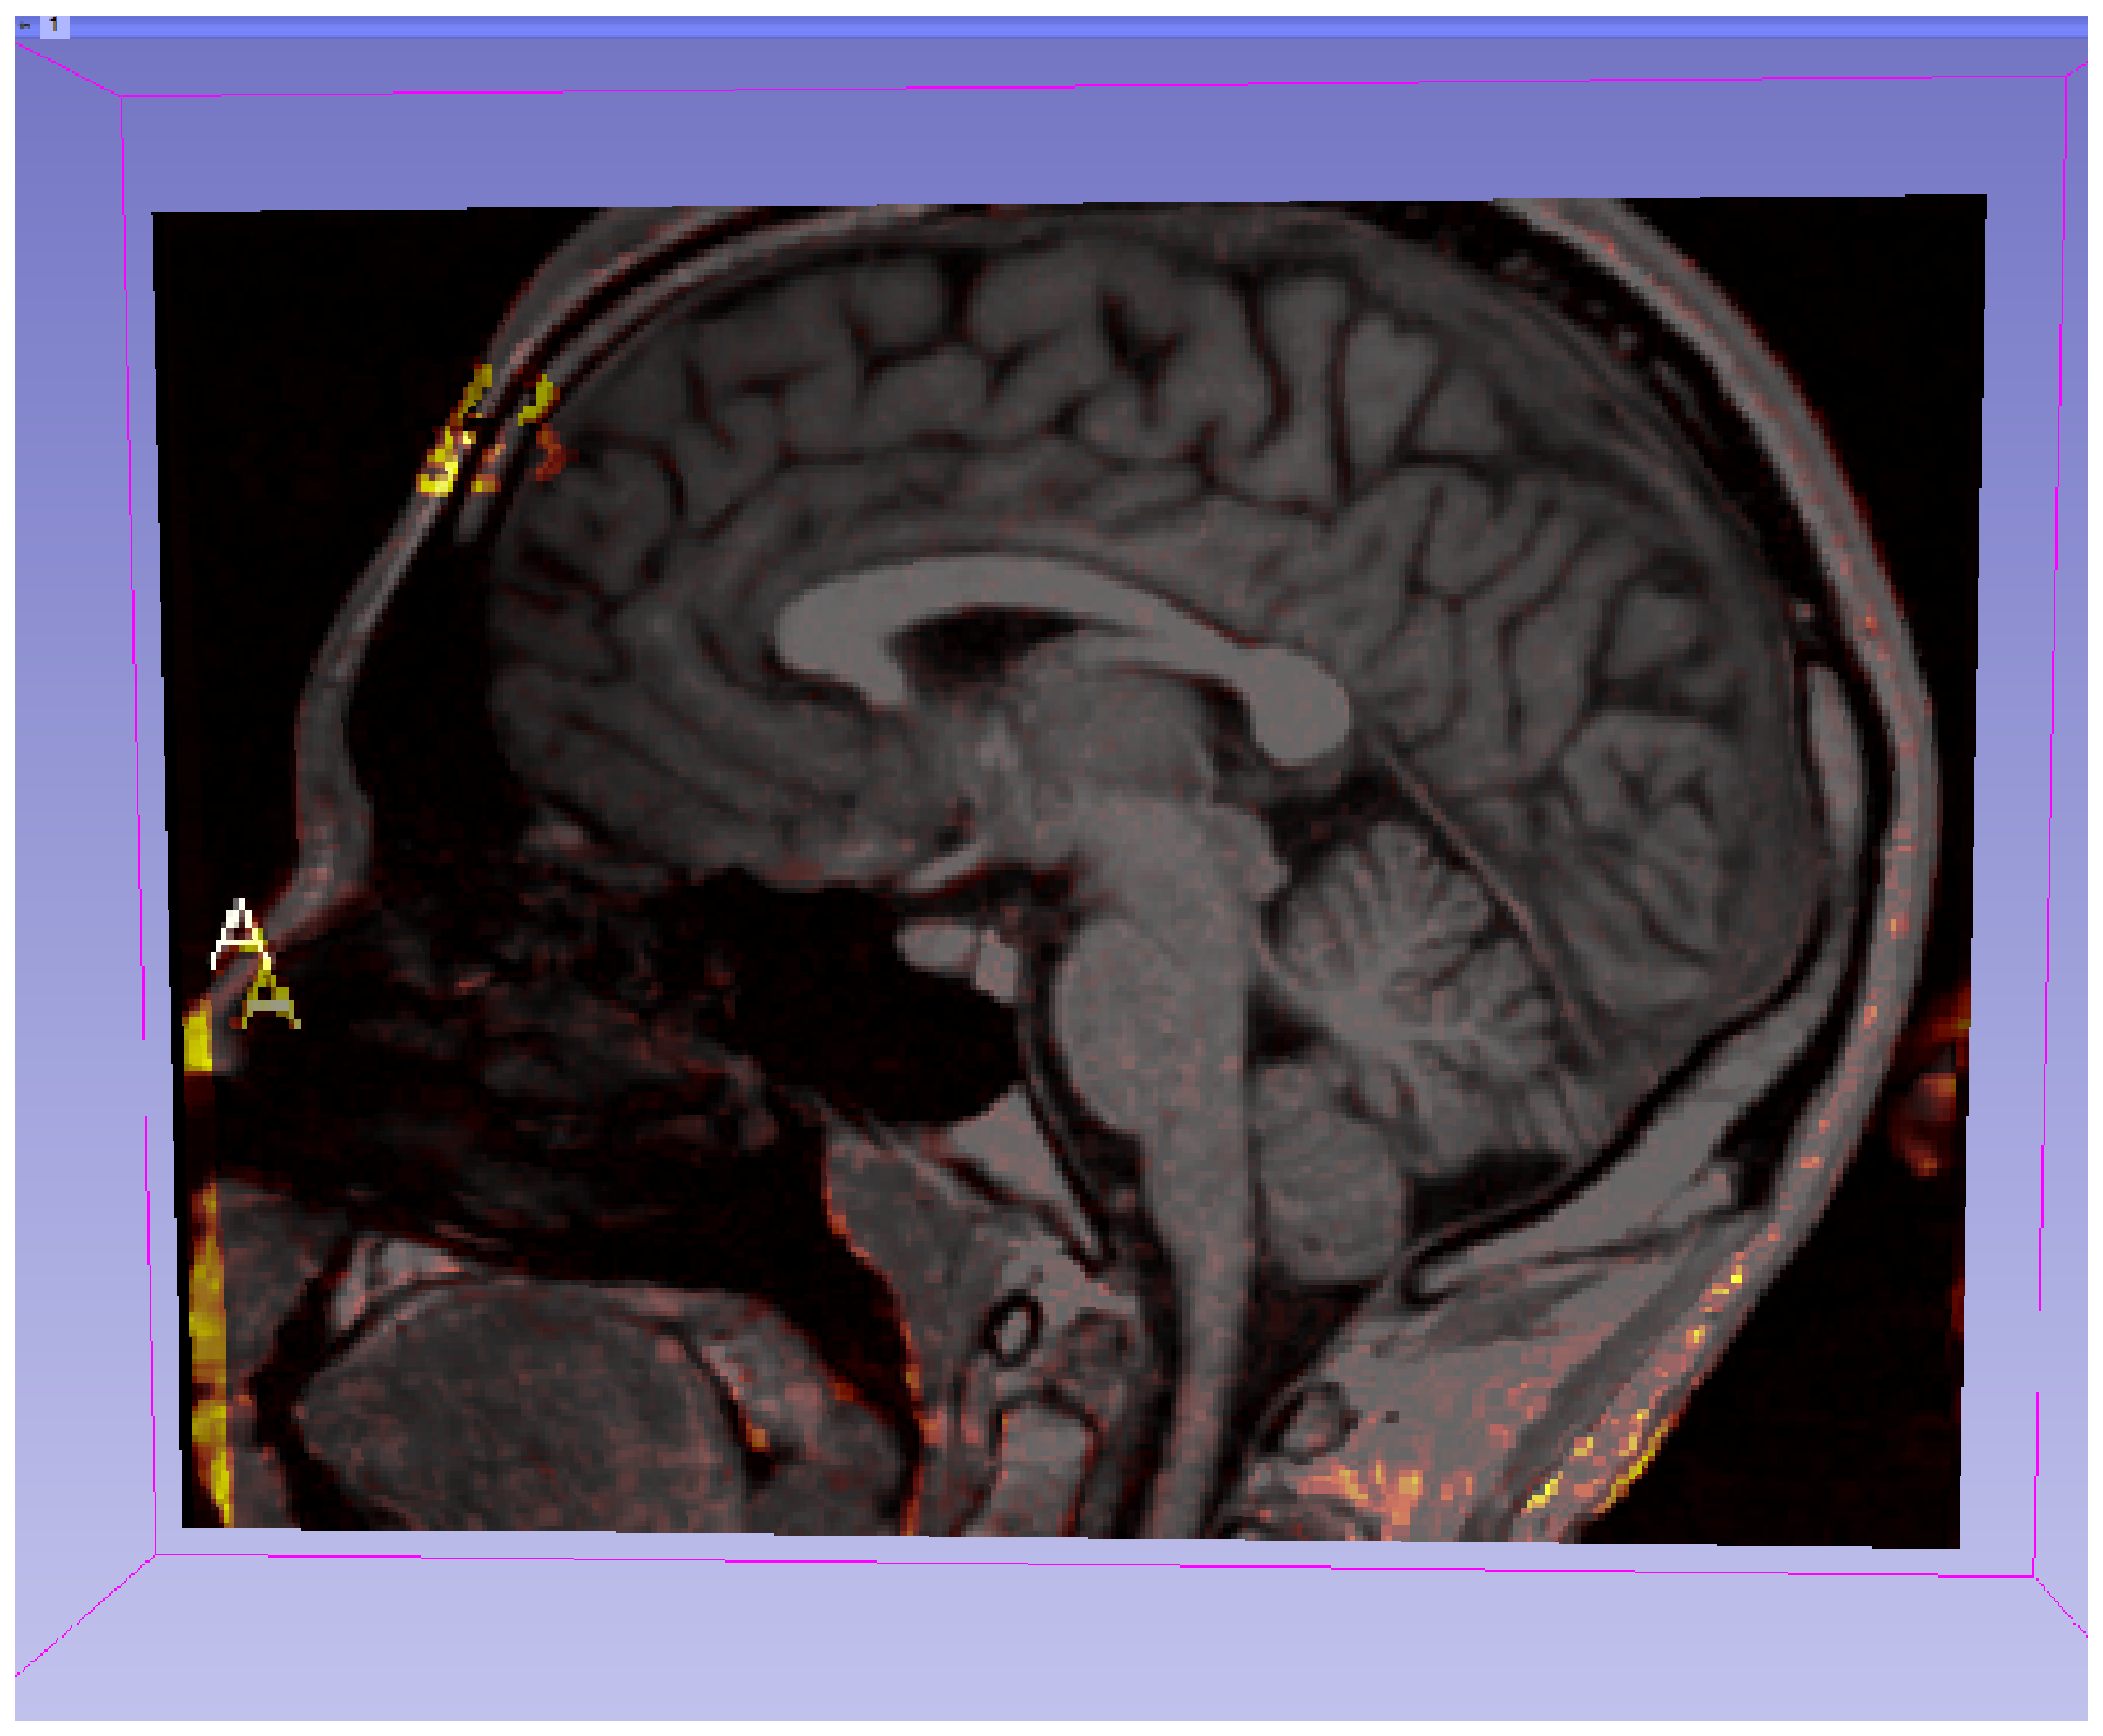
\includegraphics[scale=0.2]{/experiment_PB_P2/PB_Sagittal.eps}
  \caption{Voxel-based method. Patient 2: Sagittal plane}
  \label{PB_Sagittal}
\end{figure}


\subsubsection{Tensor-based Method}
The tensor-based method doesn't find the same differences in the corpus
callosum as the previous method. With the usual percentage values
(from $70\%$ to $80\%$ for both growth and shrinkage), the method almost
doesn't find any differences. 

In order to show some of the possible places where the method shows
some type of differences, the value of the shrinkage percentage was
increased until $88\%$. Given this, the pink areas shown are not
necessarily real differences.\\

Parameters used:
\begin{description}
\item \textit{Deformation field smoothing sigma:} 2.5
\item \textit{Shrinkage percentage:} 80
\item \textit{Growth percentage:} 88
\end{description}

\begin{figure}[H]
  \centering
  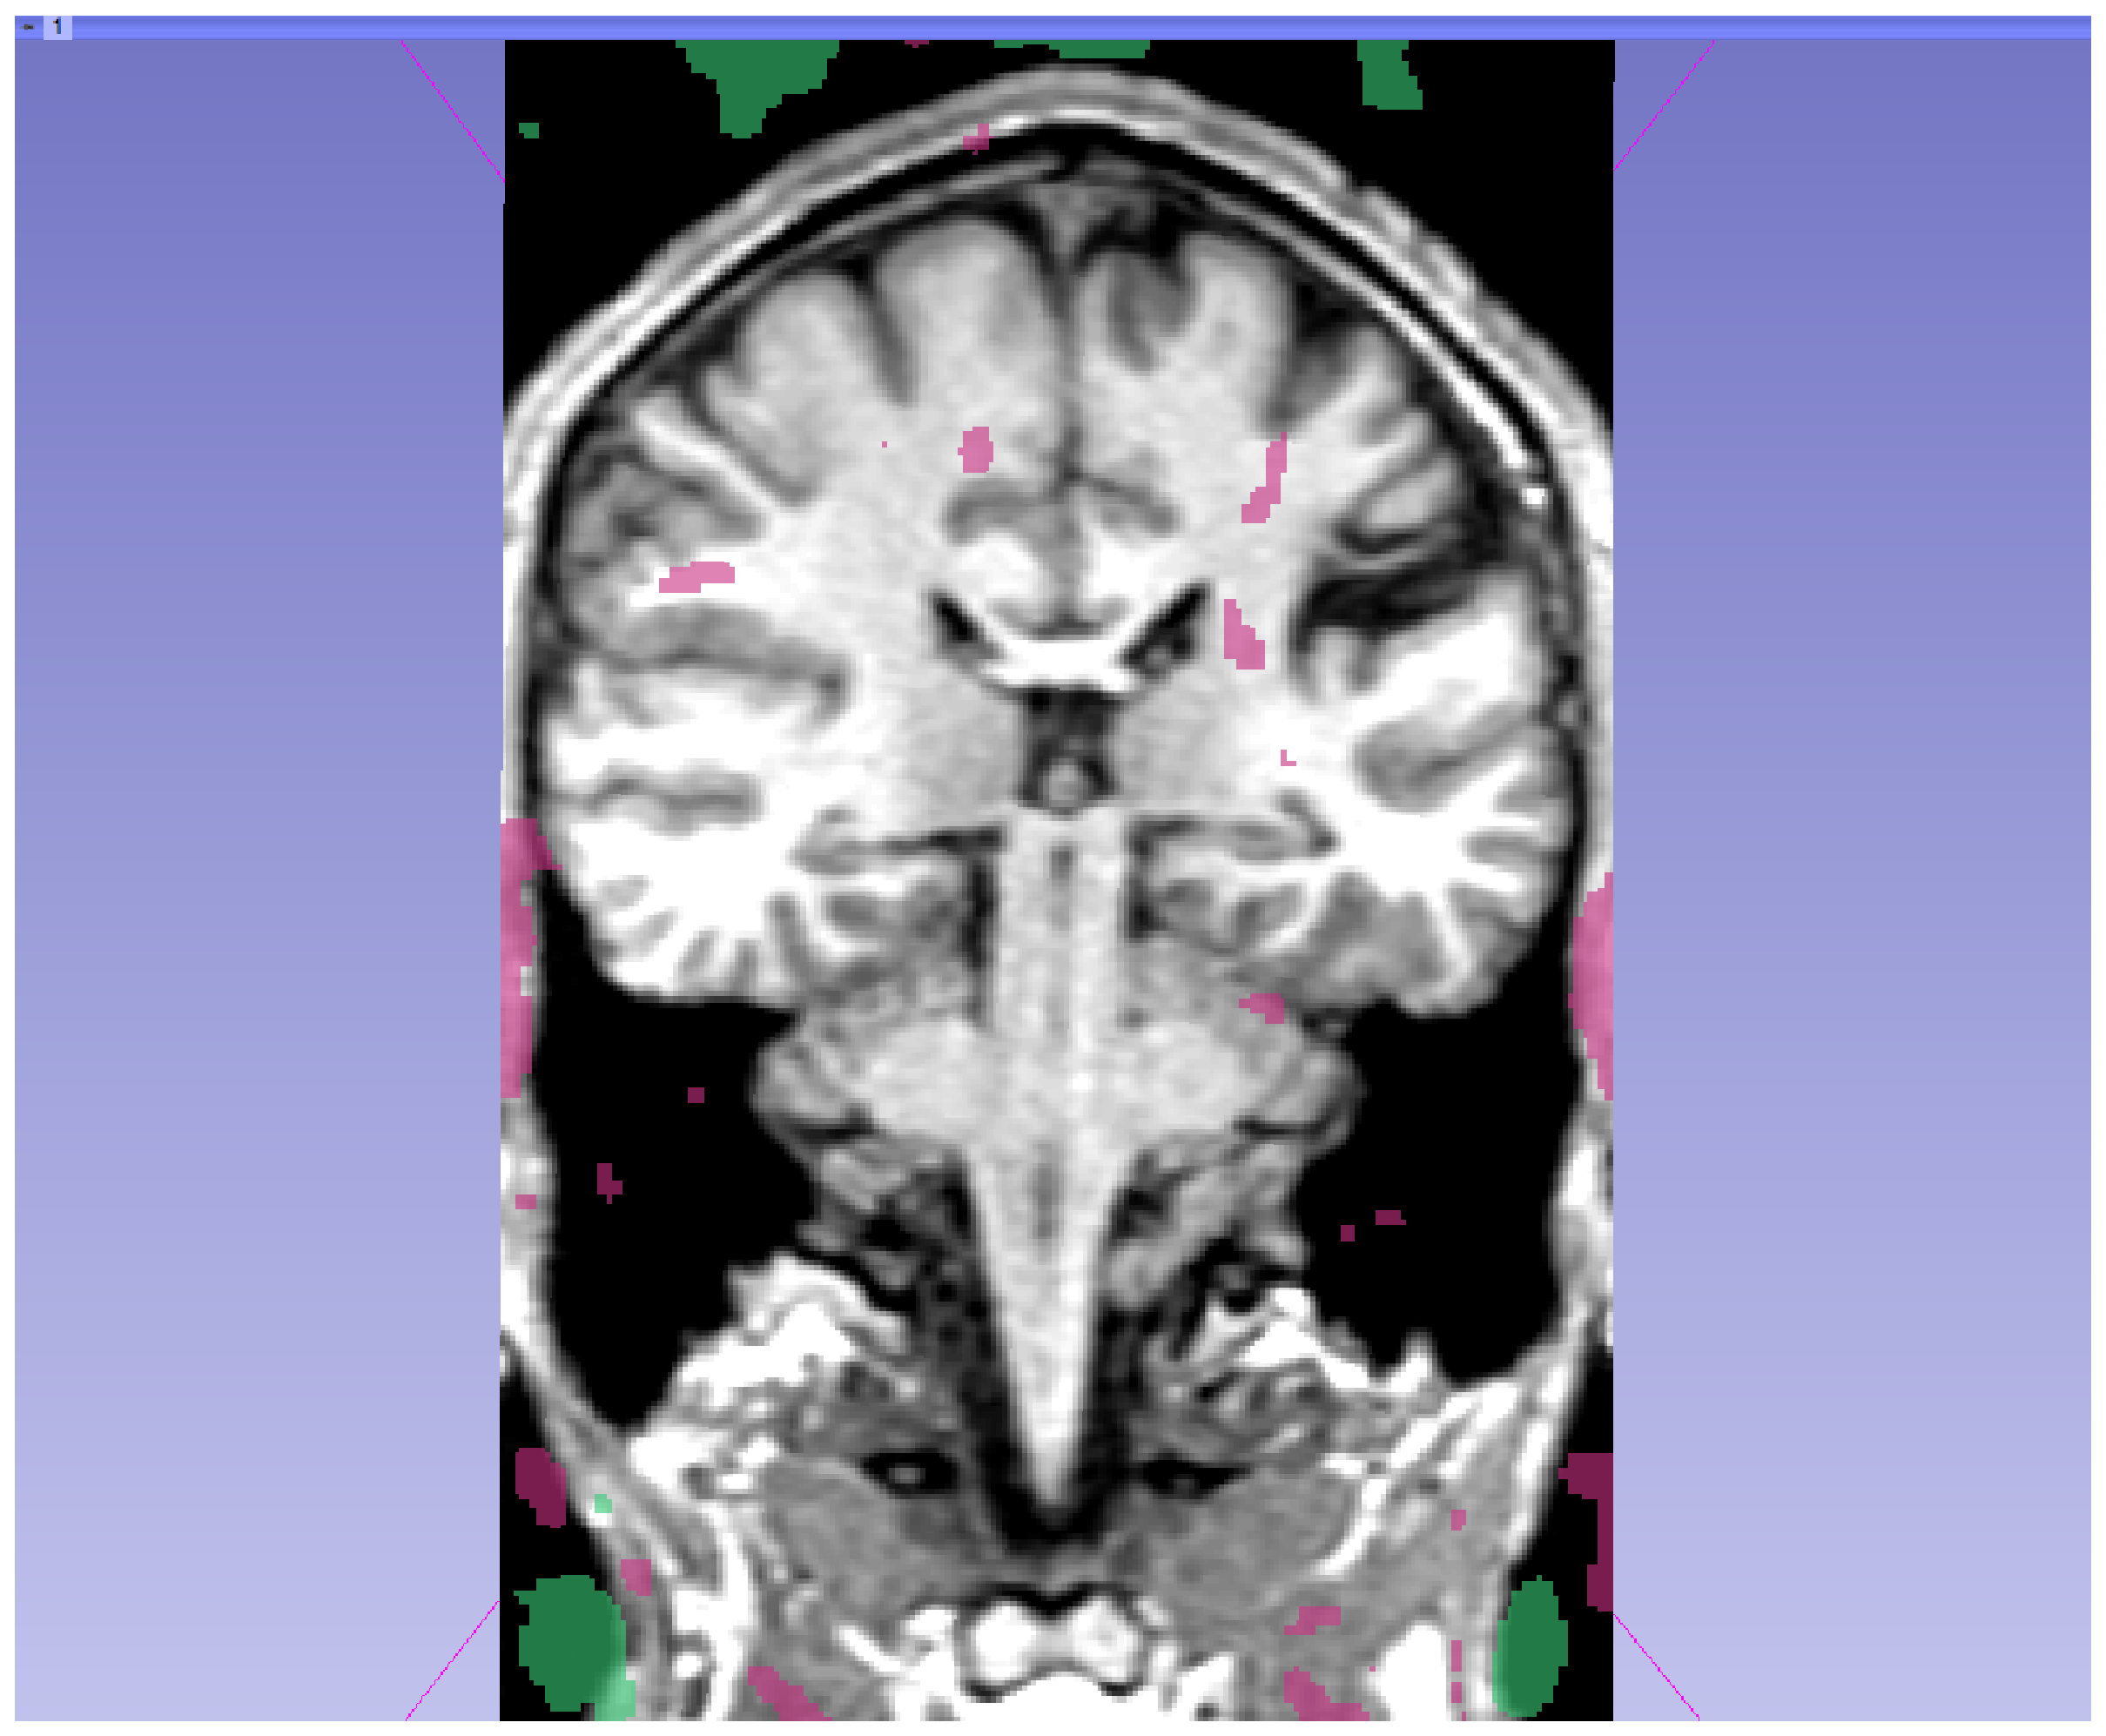
\includegraphics[scale=0.2]{/experiment_PB_P2/PB_Tensor_Coronal.eps}
  \caption{Tensor-based method. Patient 2: Coronal plane}
  \label{PB_TCoronal}
\end{figure}

\begin{figure}[H]
  \centering
  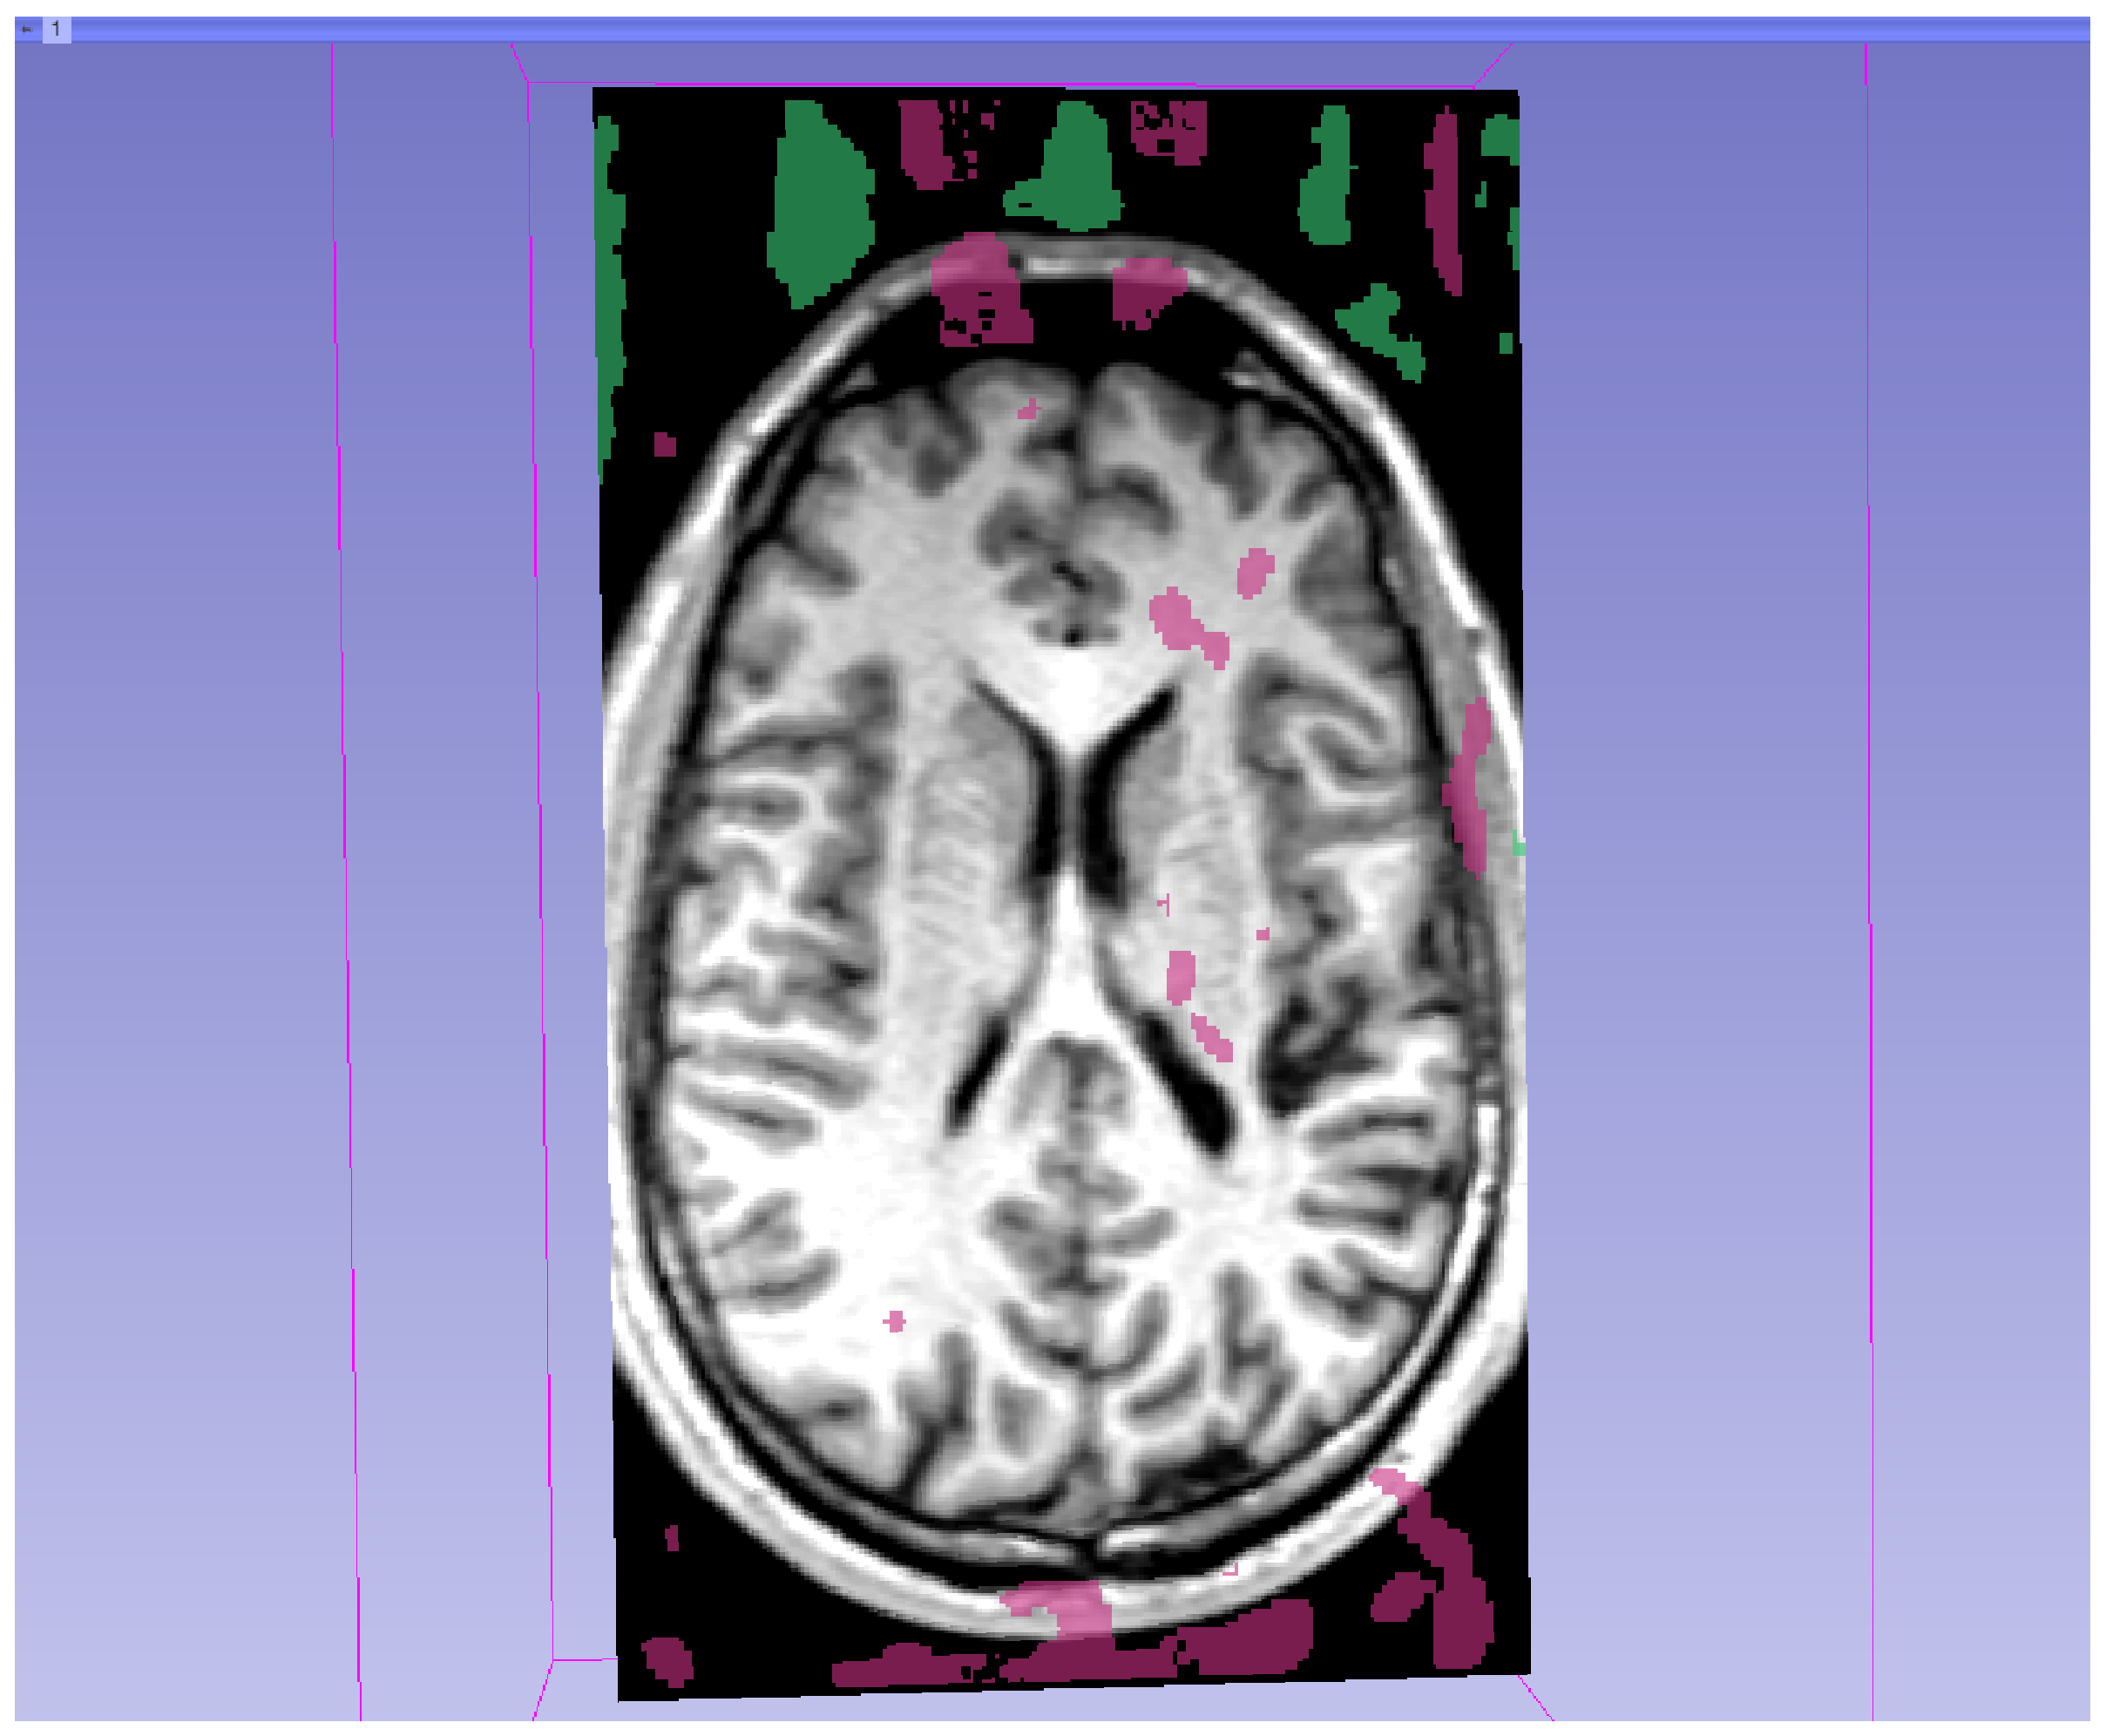
\includegraphics[scale=0.2]{/experiment_PB_P2/PB_Tensor_Traversal.eps}
  \caption{Tensor-based method. Patient 2: Traversal plane}
  \label{PB_TTraversal}
\end{figure}

\begin{figure}[H]
  \centering
  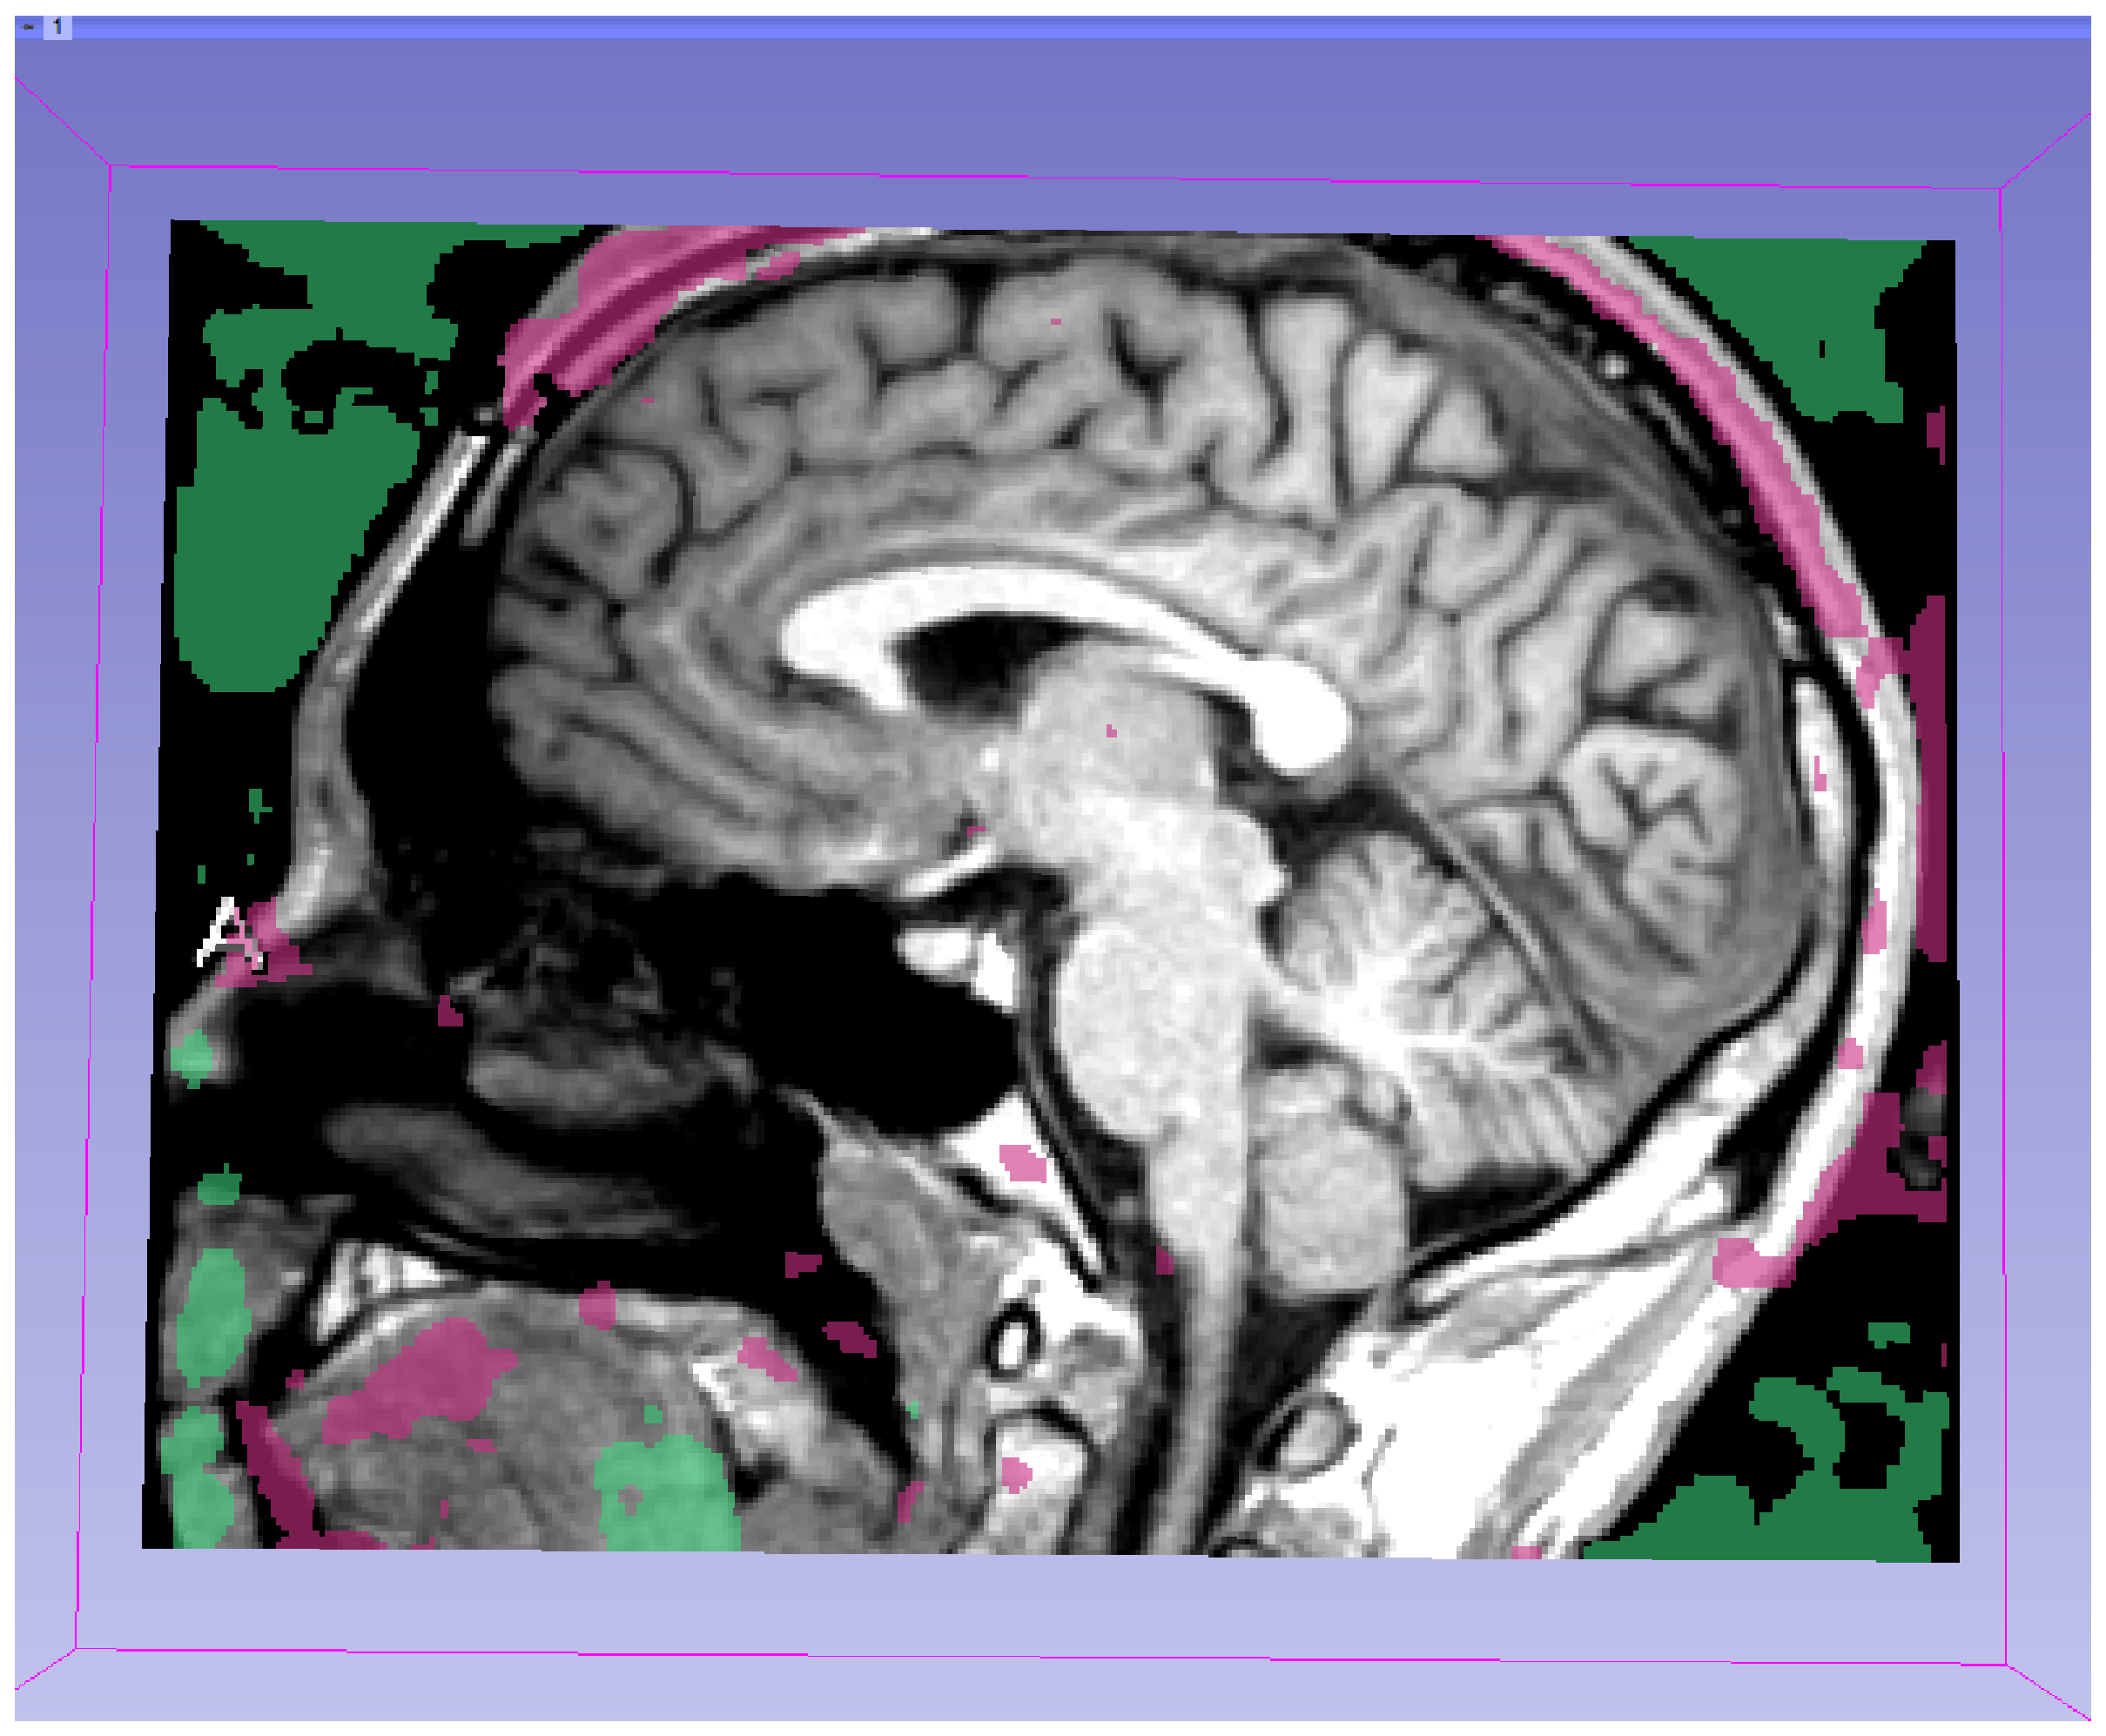
\includegraphics[scale=0.2]{/experiment_PB_P2/PB_Tensor_Sagittal.eps}
  \caption{Tensor-based method. Patient 2: Sagittal plane}
  \label{PB_TSagittal}
\end{figure}


\subsection{Patient 3}
This patient had a medical condition for which it has had two
surgeries performed. A tumor, located on the right hemisphere of the
frontal lobe, was removed during the first surgery. The MRIs used
during this experiment were taken before and after the second surgery,
in which a second growth was removed located the same area.


\subsubsection{Voxel-based Method}
The method shows the expected differences in the right hemisphere of
the frontal lobe of the brain. It also shows some size differences
especially in the lower parietal lobe, which can be observed in image
\ref{B2_Traversal1}.\\

The registration method used was \textit{Affine registration}.

\begin{figure}[H]
  \centering
  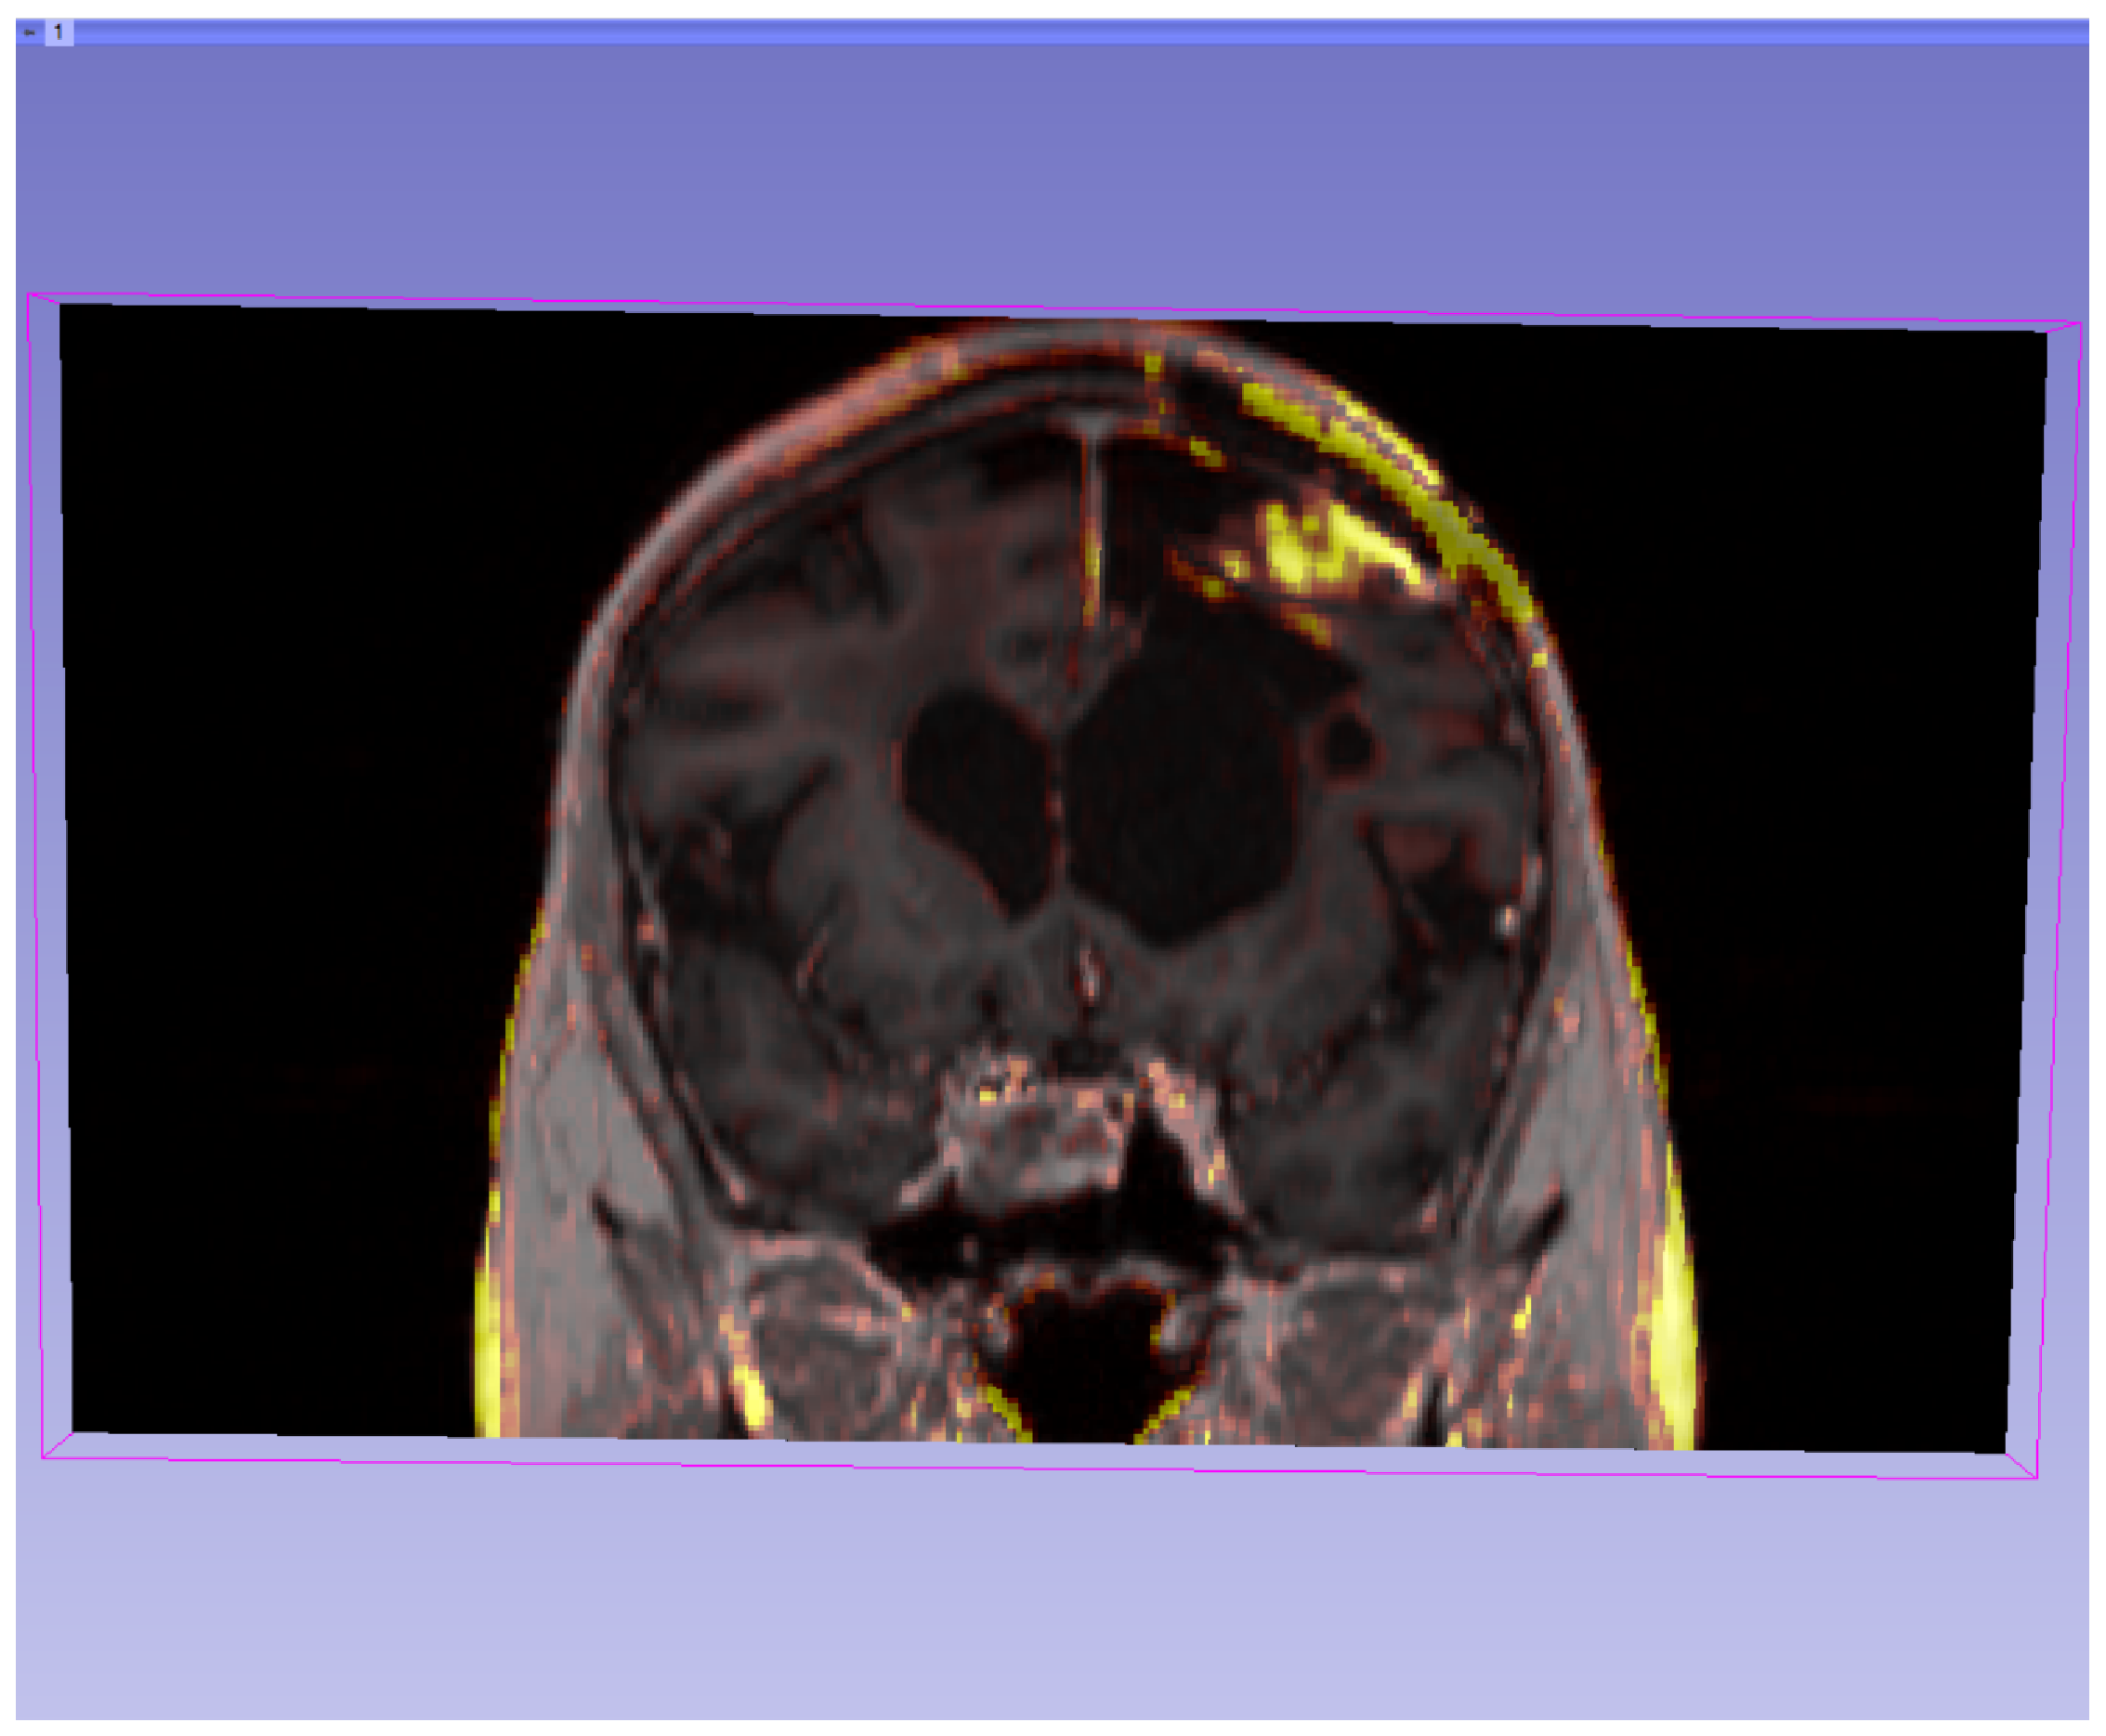
\includegraphics[scale=0.2]{/experiment_B2_P3/B2_Coronal.eps}
  \caption{Voxel-based method. Patient 3: Coronal plane}
  \label{B2_Coronal}
\end{figure}

\begin{figure}[H]
  \centering
  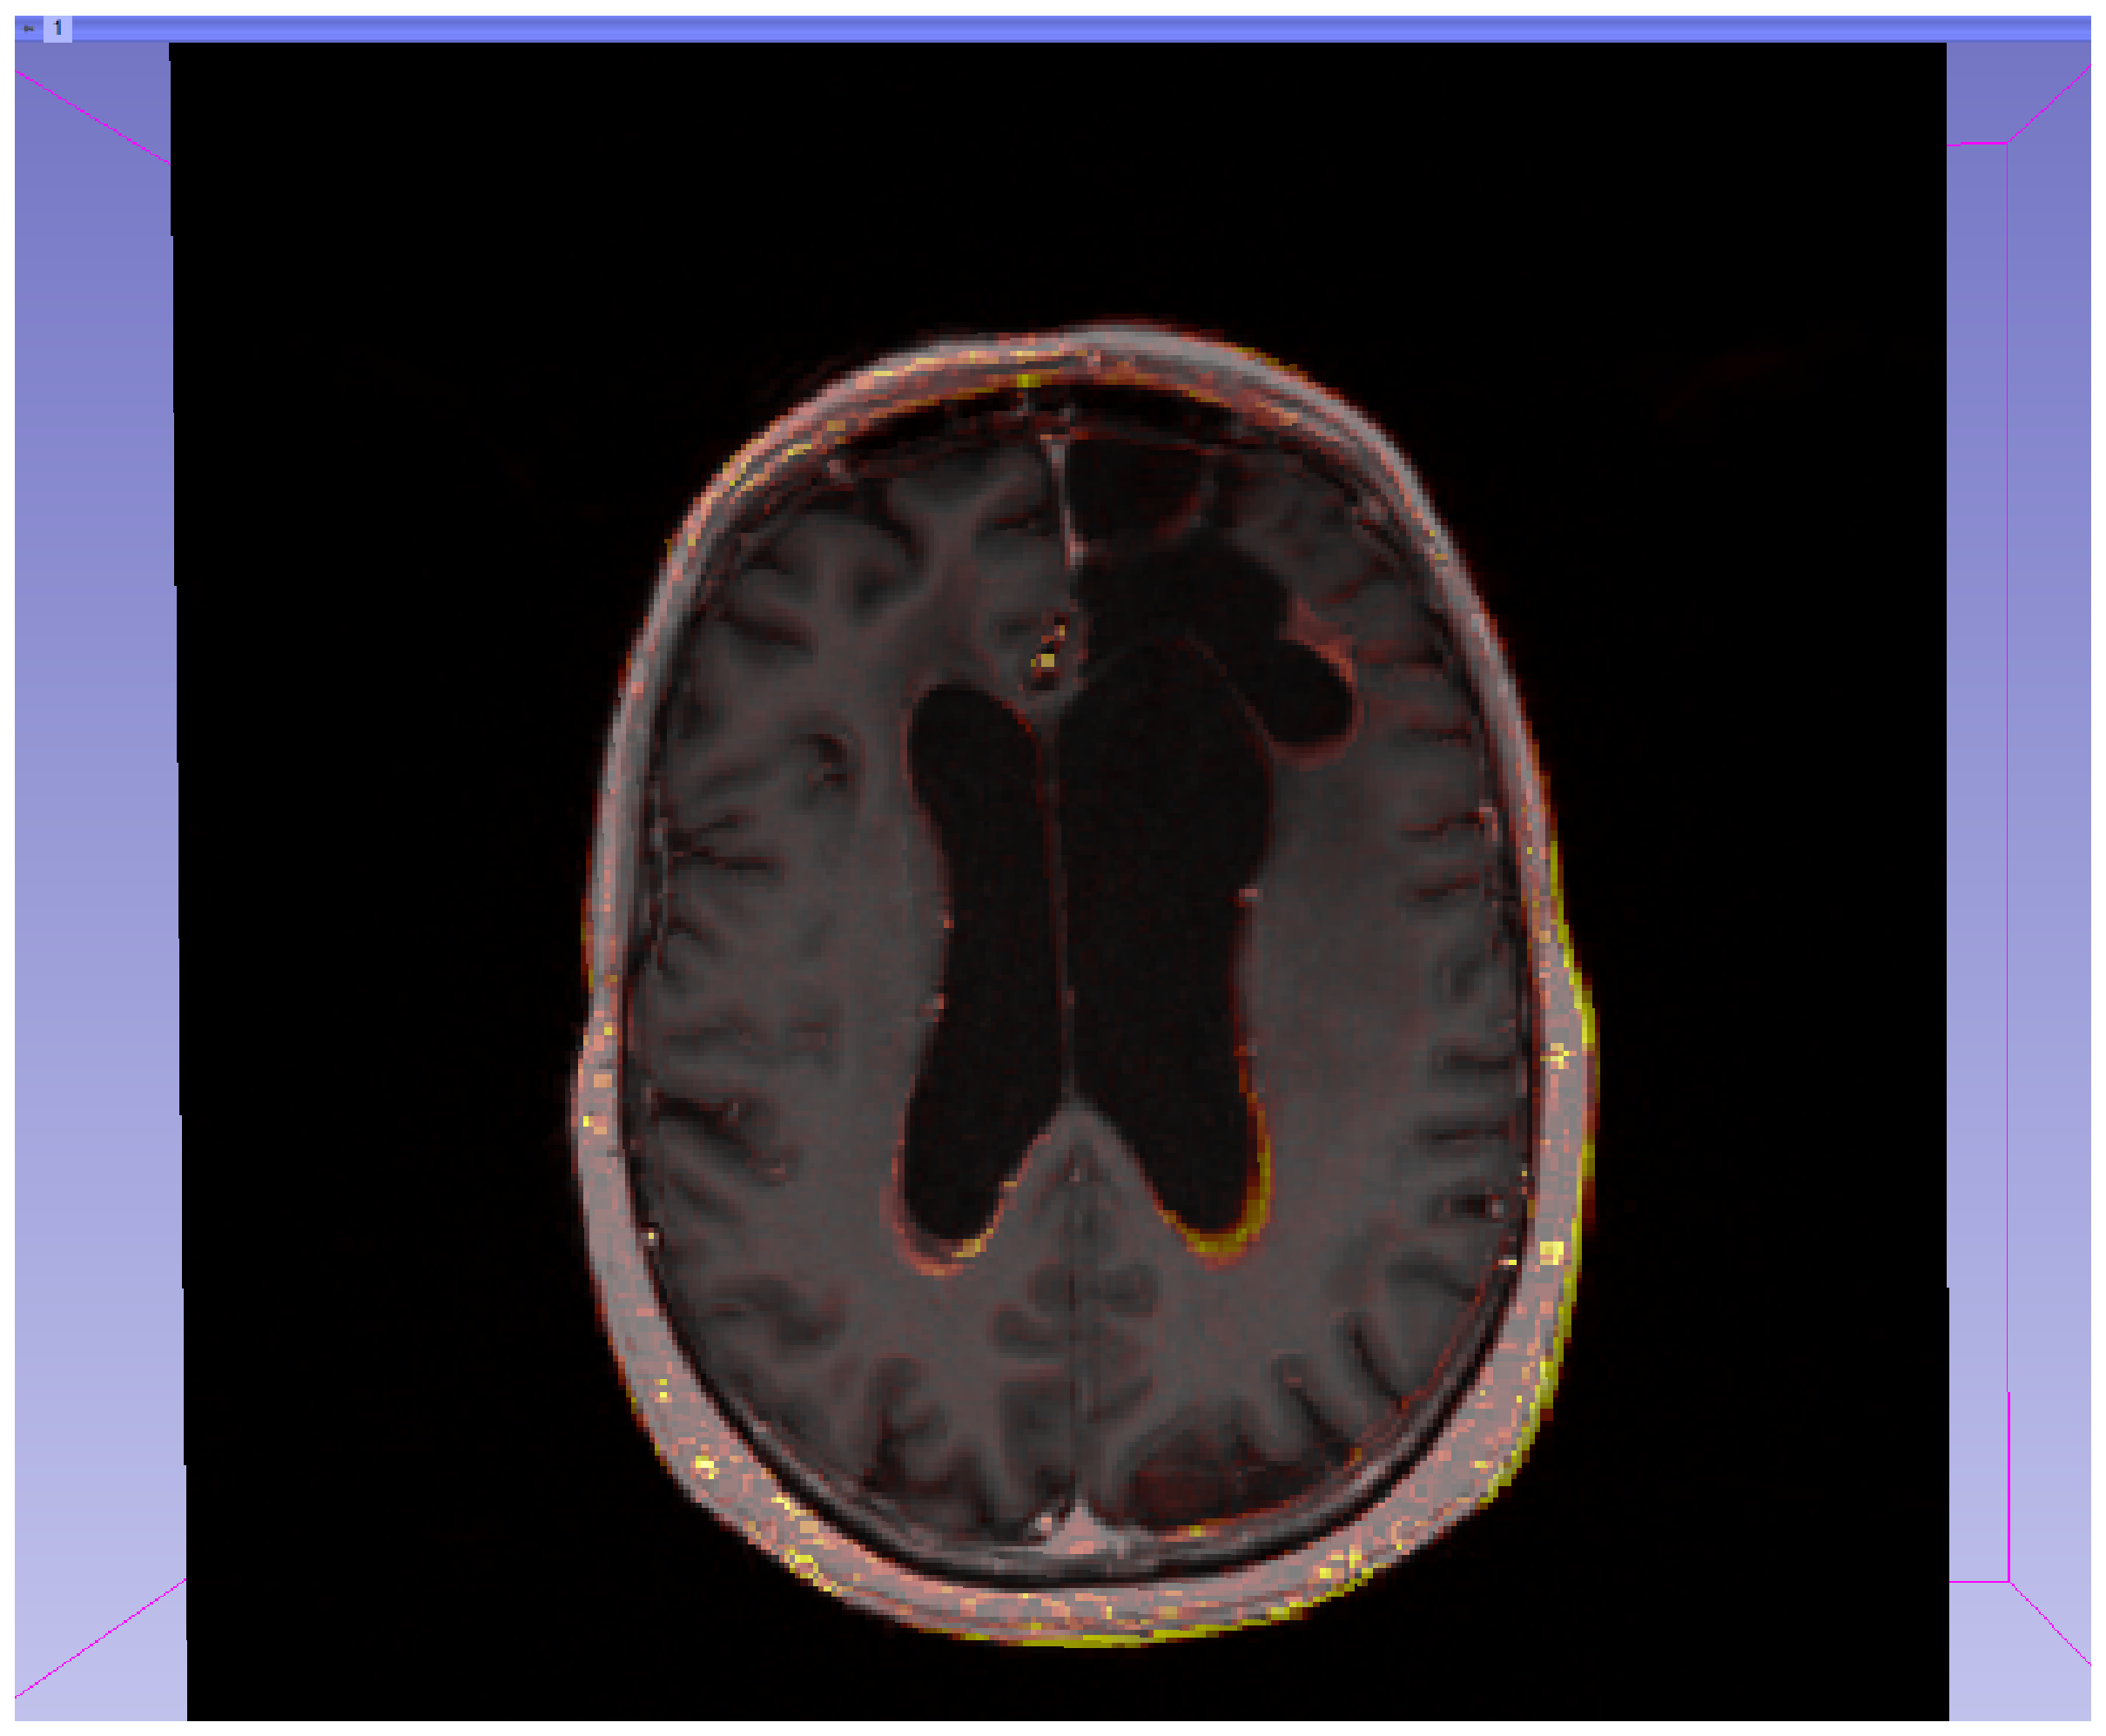
\includegraphics[scale=0.2]{/experiment_B2_P3/B2_Traversal1.eps}
  \caption{Voxel-based method. Patient 3: Traversal plane}
  \label{B2_Traversal1}
\end{figure}

\begin{figure}[H]
  \centering
  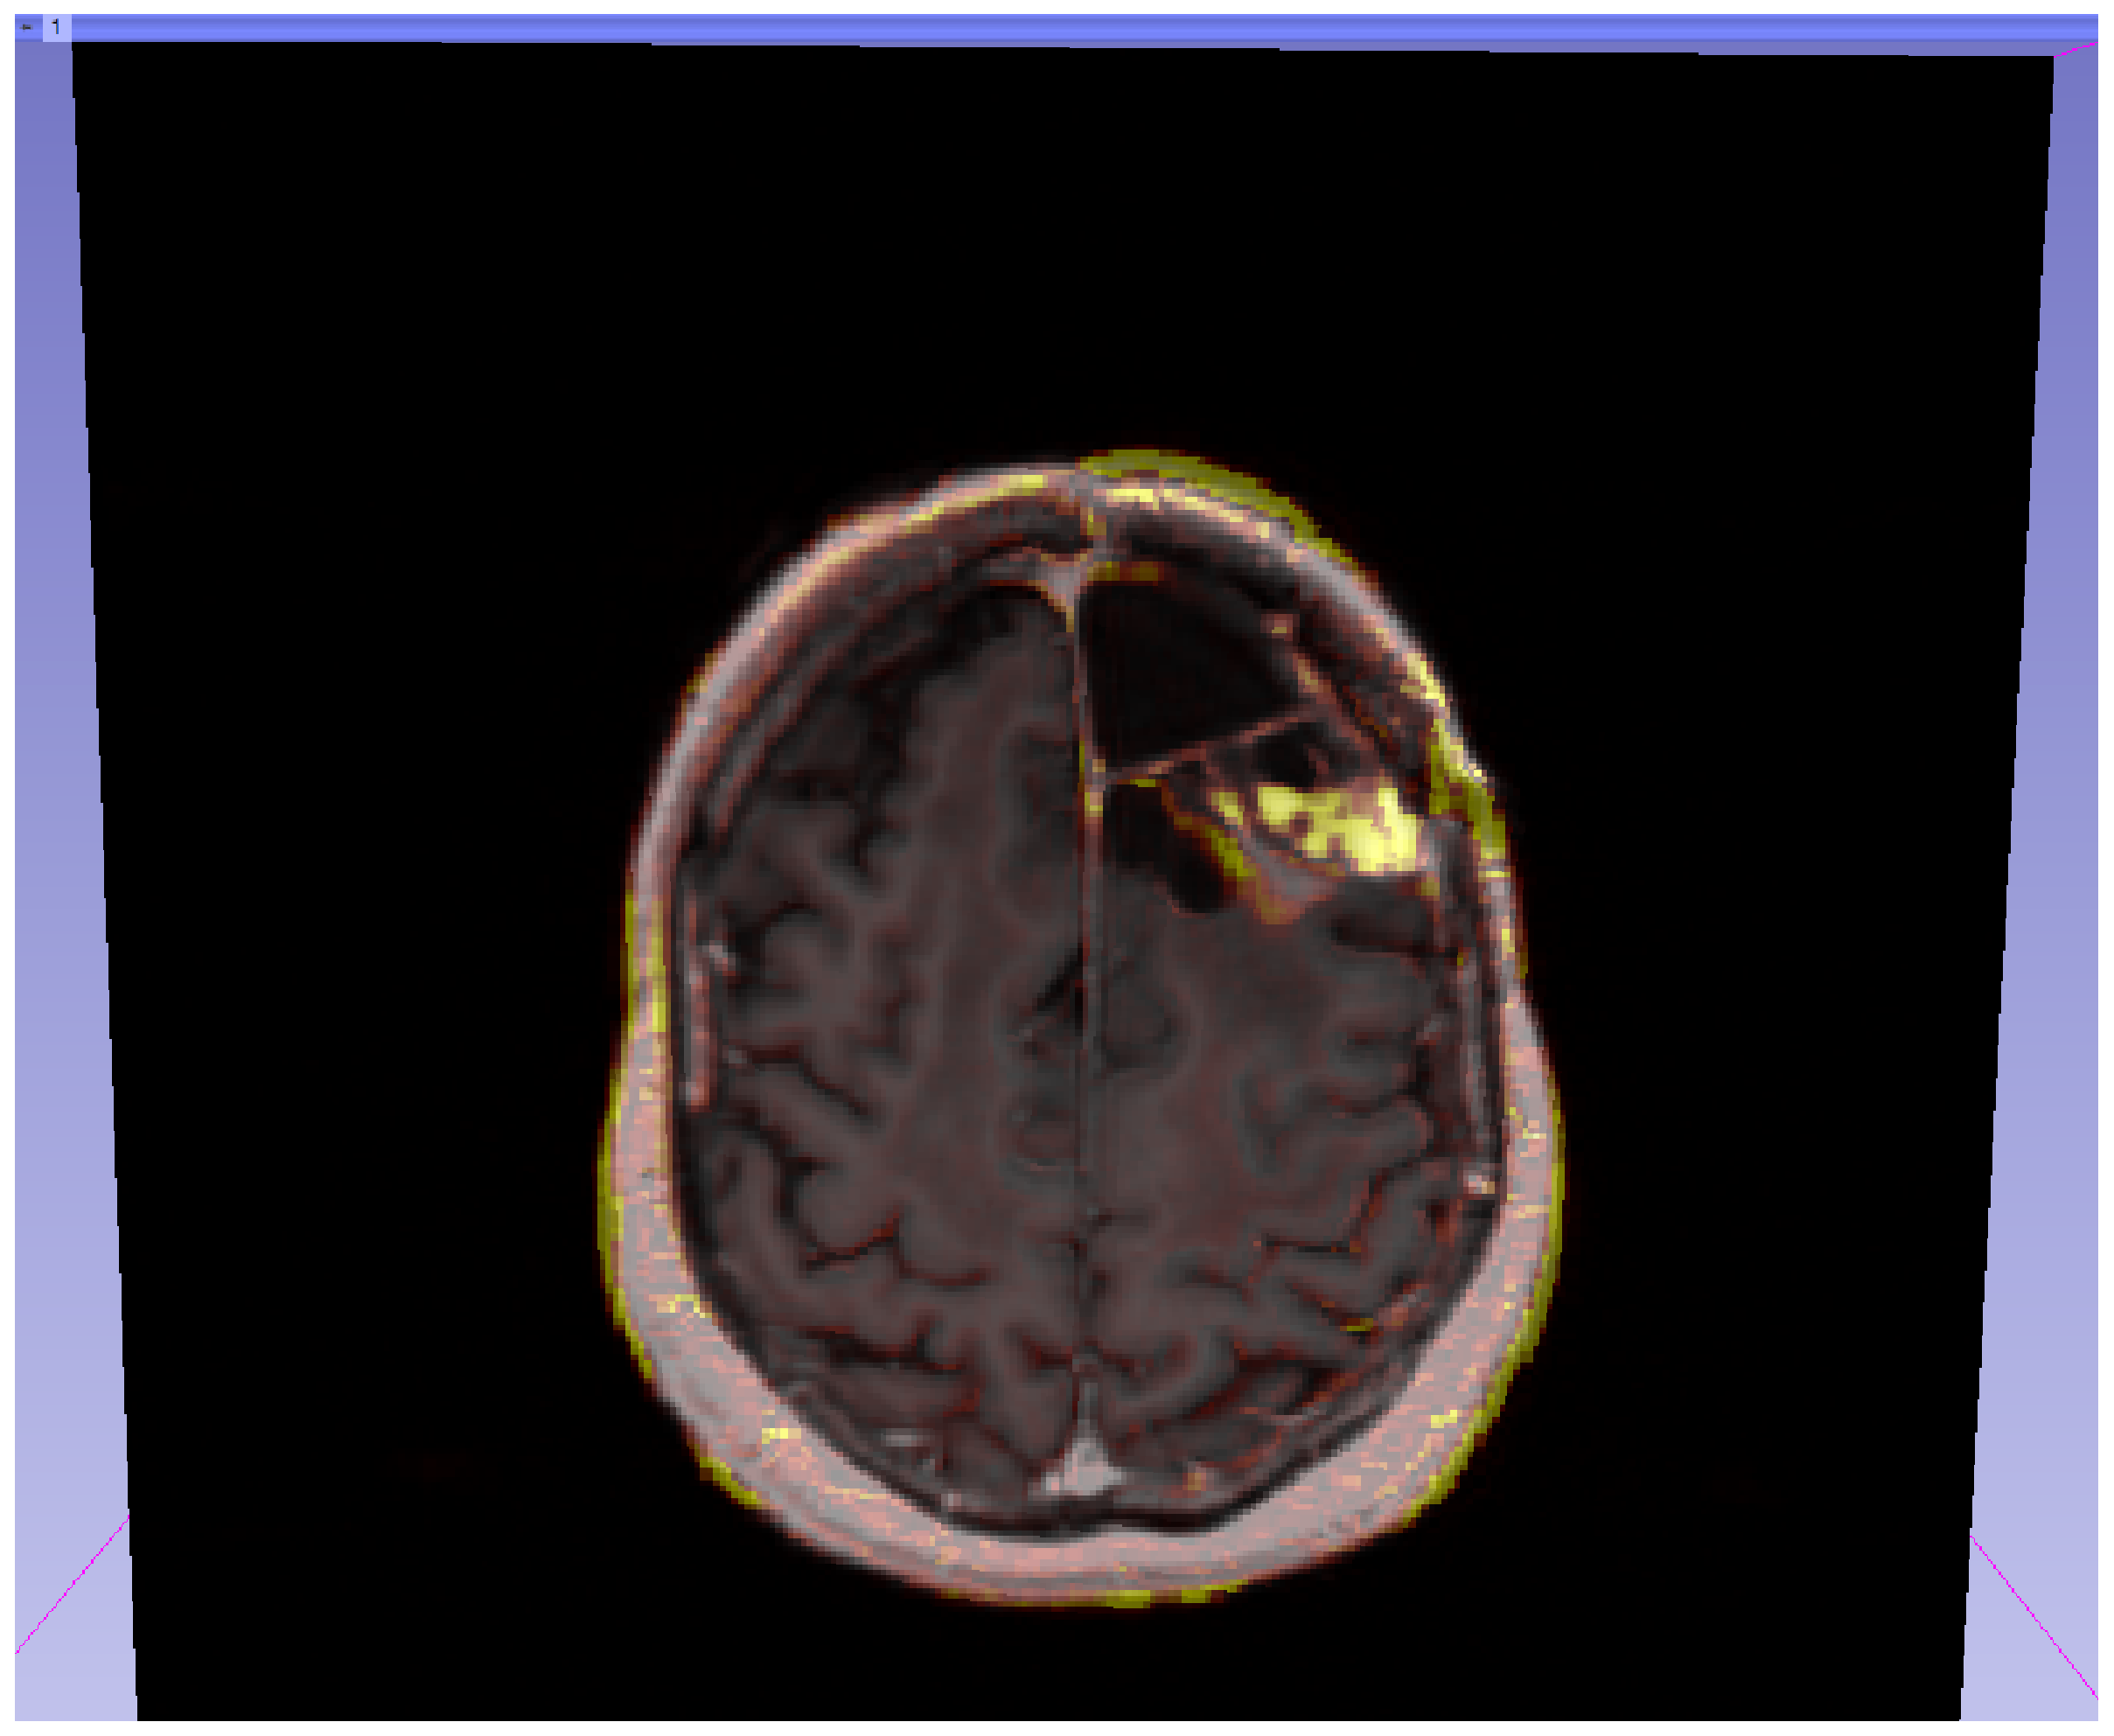
\includegraphics[scale=0.2]{/experiment_B2_P3/B2_Traversal2.eps}
  \caption{Voxel-based method. Patient 3: Upper traversal plane}
  \label{B2_Traversal2}
\end{figure}

\begin{figure}[H]
  \centering
  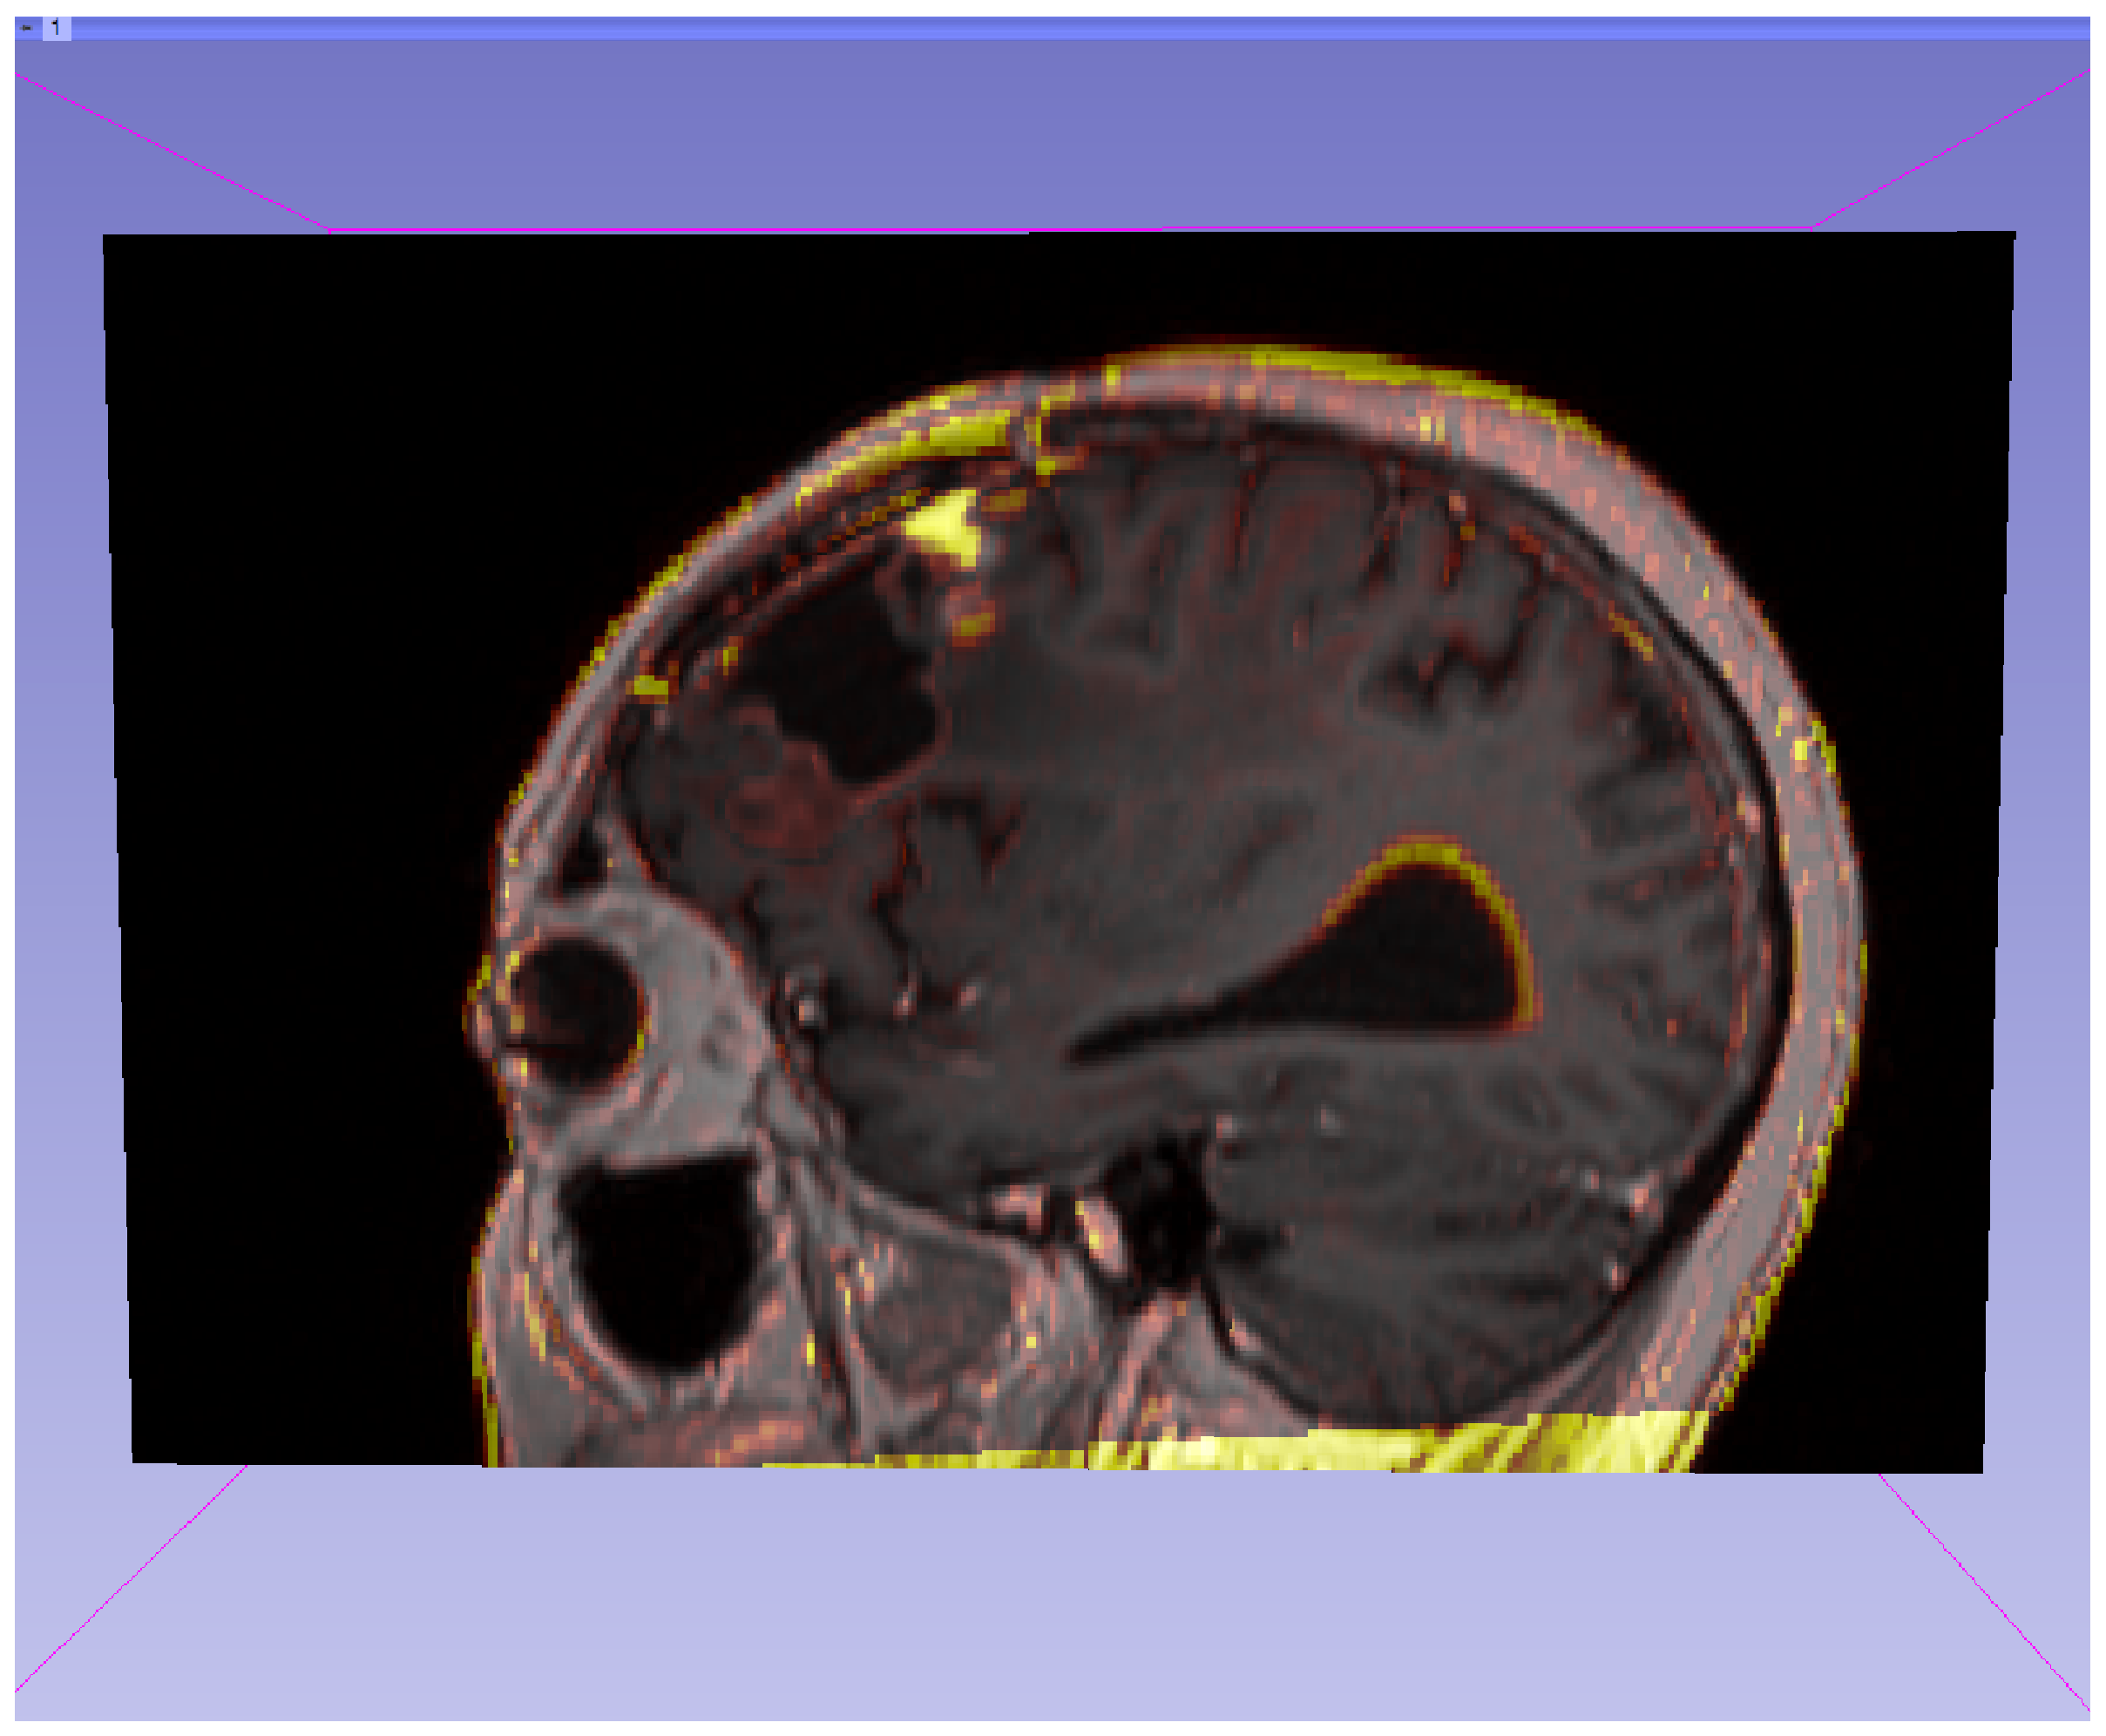
\includegraphics[scale=0.2]{/experiment_B2_P3/B2_Sagittal.eps}
  \caption{Voxel-based method. Patient 3: Sagittal plane}
  \label{B2_Sagittal}
\end{figure}


\subsubsection{Tensor-based Method}
This method also shows the expected difference due to the surgery
(correctly expressed as shrinkage, in green) which can be seen in the
images \ref{B2_TCoronal}, \ref{B2_TTraversal2} and \ref{B2_TSagittal}.

The image \ref{B2_TTraversal1} is showed for comparison with the
differences shown in image \ref{B2_Traversal1} in the previous
method. The tensor-based result doesn't show the exact same result;
however, some growth (in pink) can be seen. This could be attributed
to either inaccuracy of the method or to movement in the brain
consistent with the surgery.\\

Parameters used:
\begin{description}
\item \textit{Deformation field smoothing sigma:} 2.5
\item \textit{Shrinkage percentage:} 60
\item \textit{Growth percentage:} 50
\end{description}

\begin{figure}[H]
  \centering
  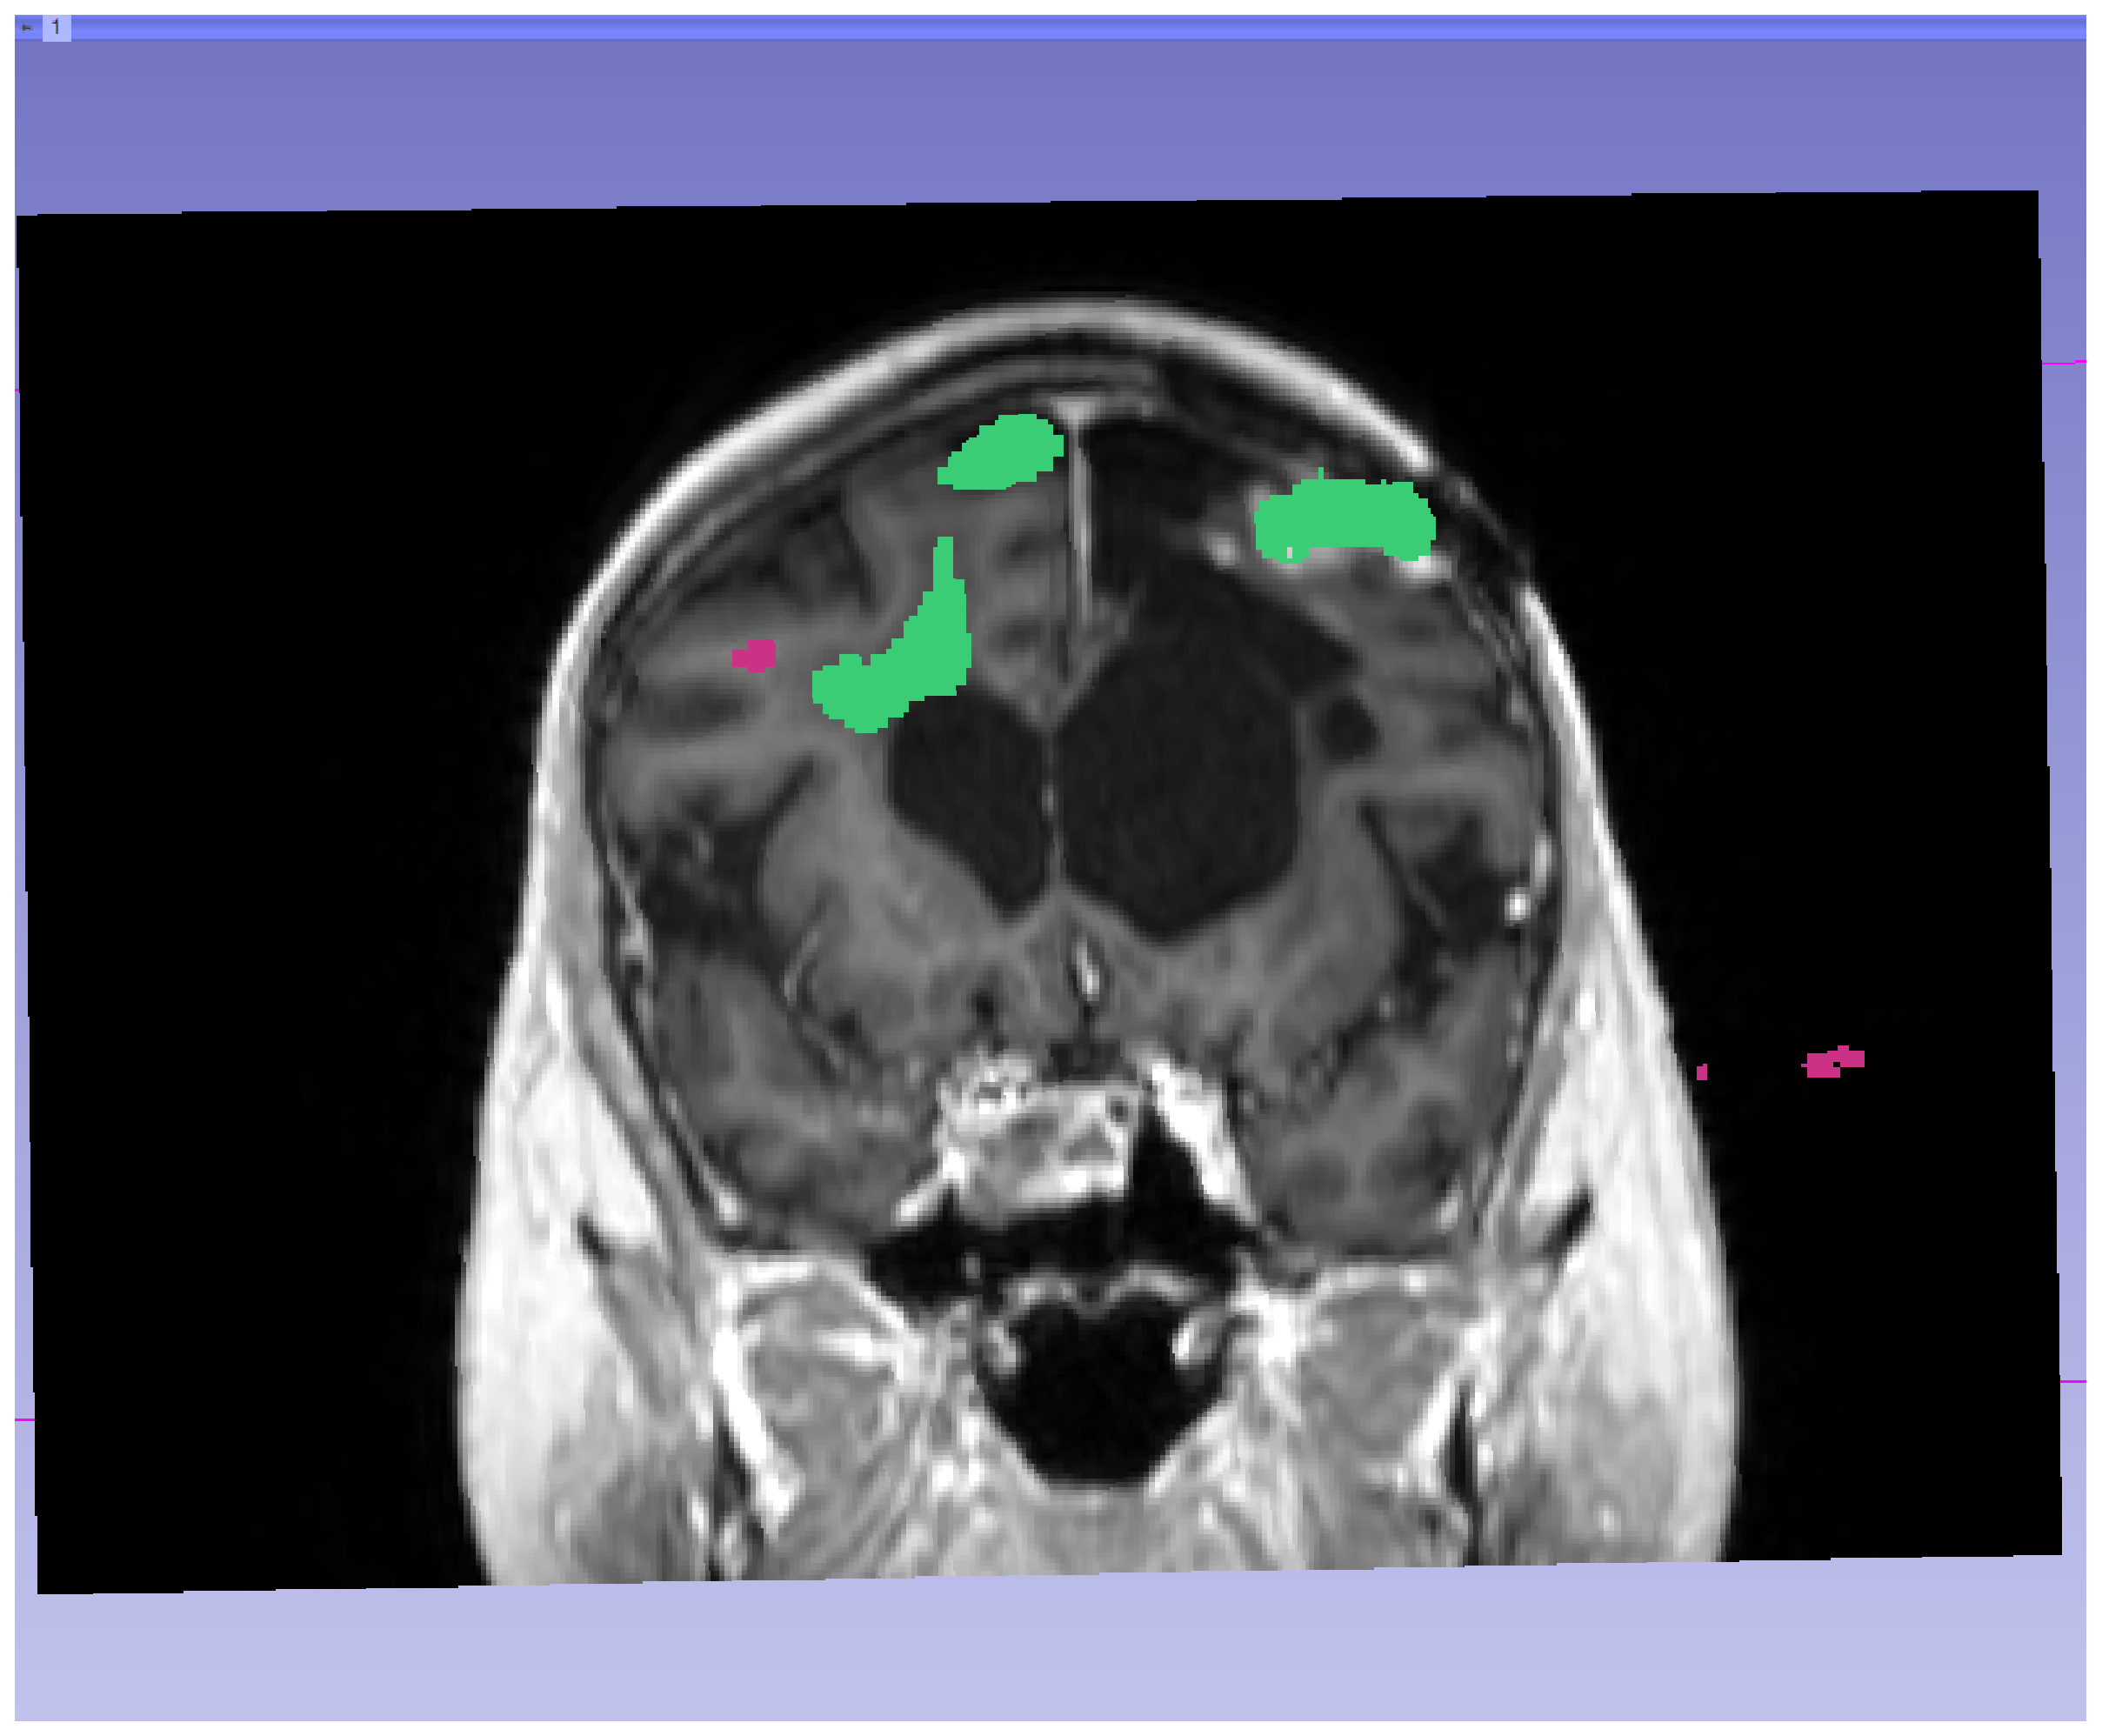
\includegraphics[scale=0.2]{/experiment_B2_P3/B2_Tensor_Coronal.eps}
  \caption{Tensor-based method. Patient 3: Coronal plane}
  \label{B2_TCoronal}
\end{figure}

\begin{figure}[H]
  \centering
  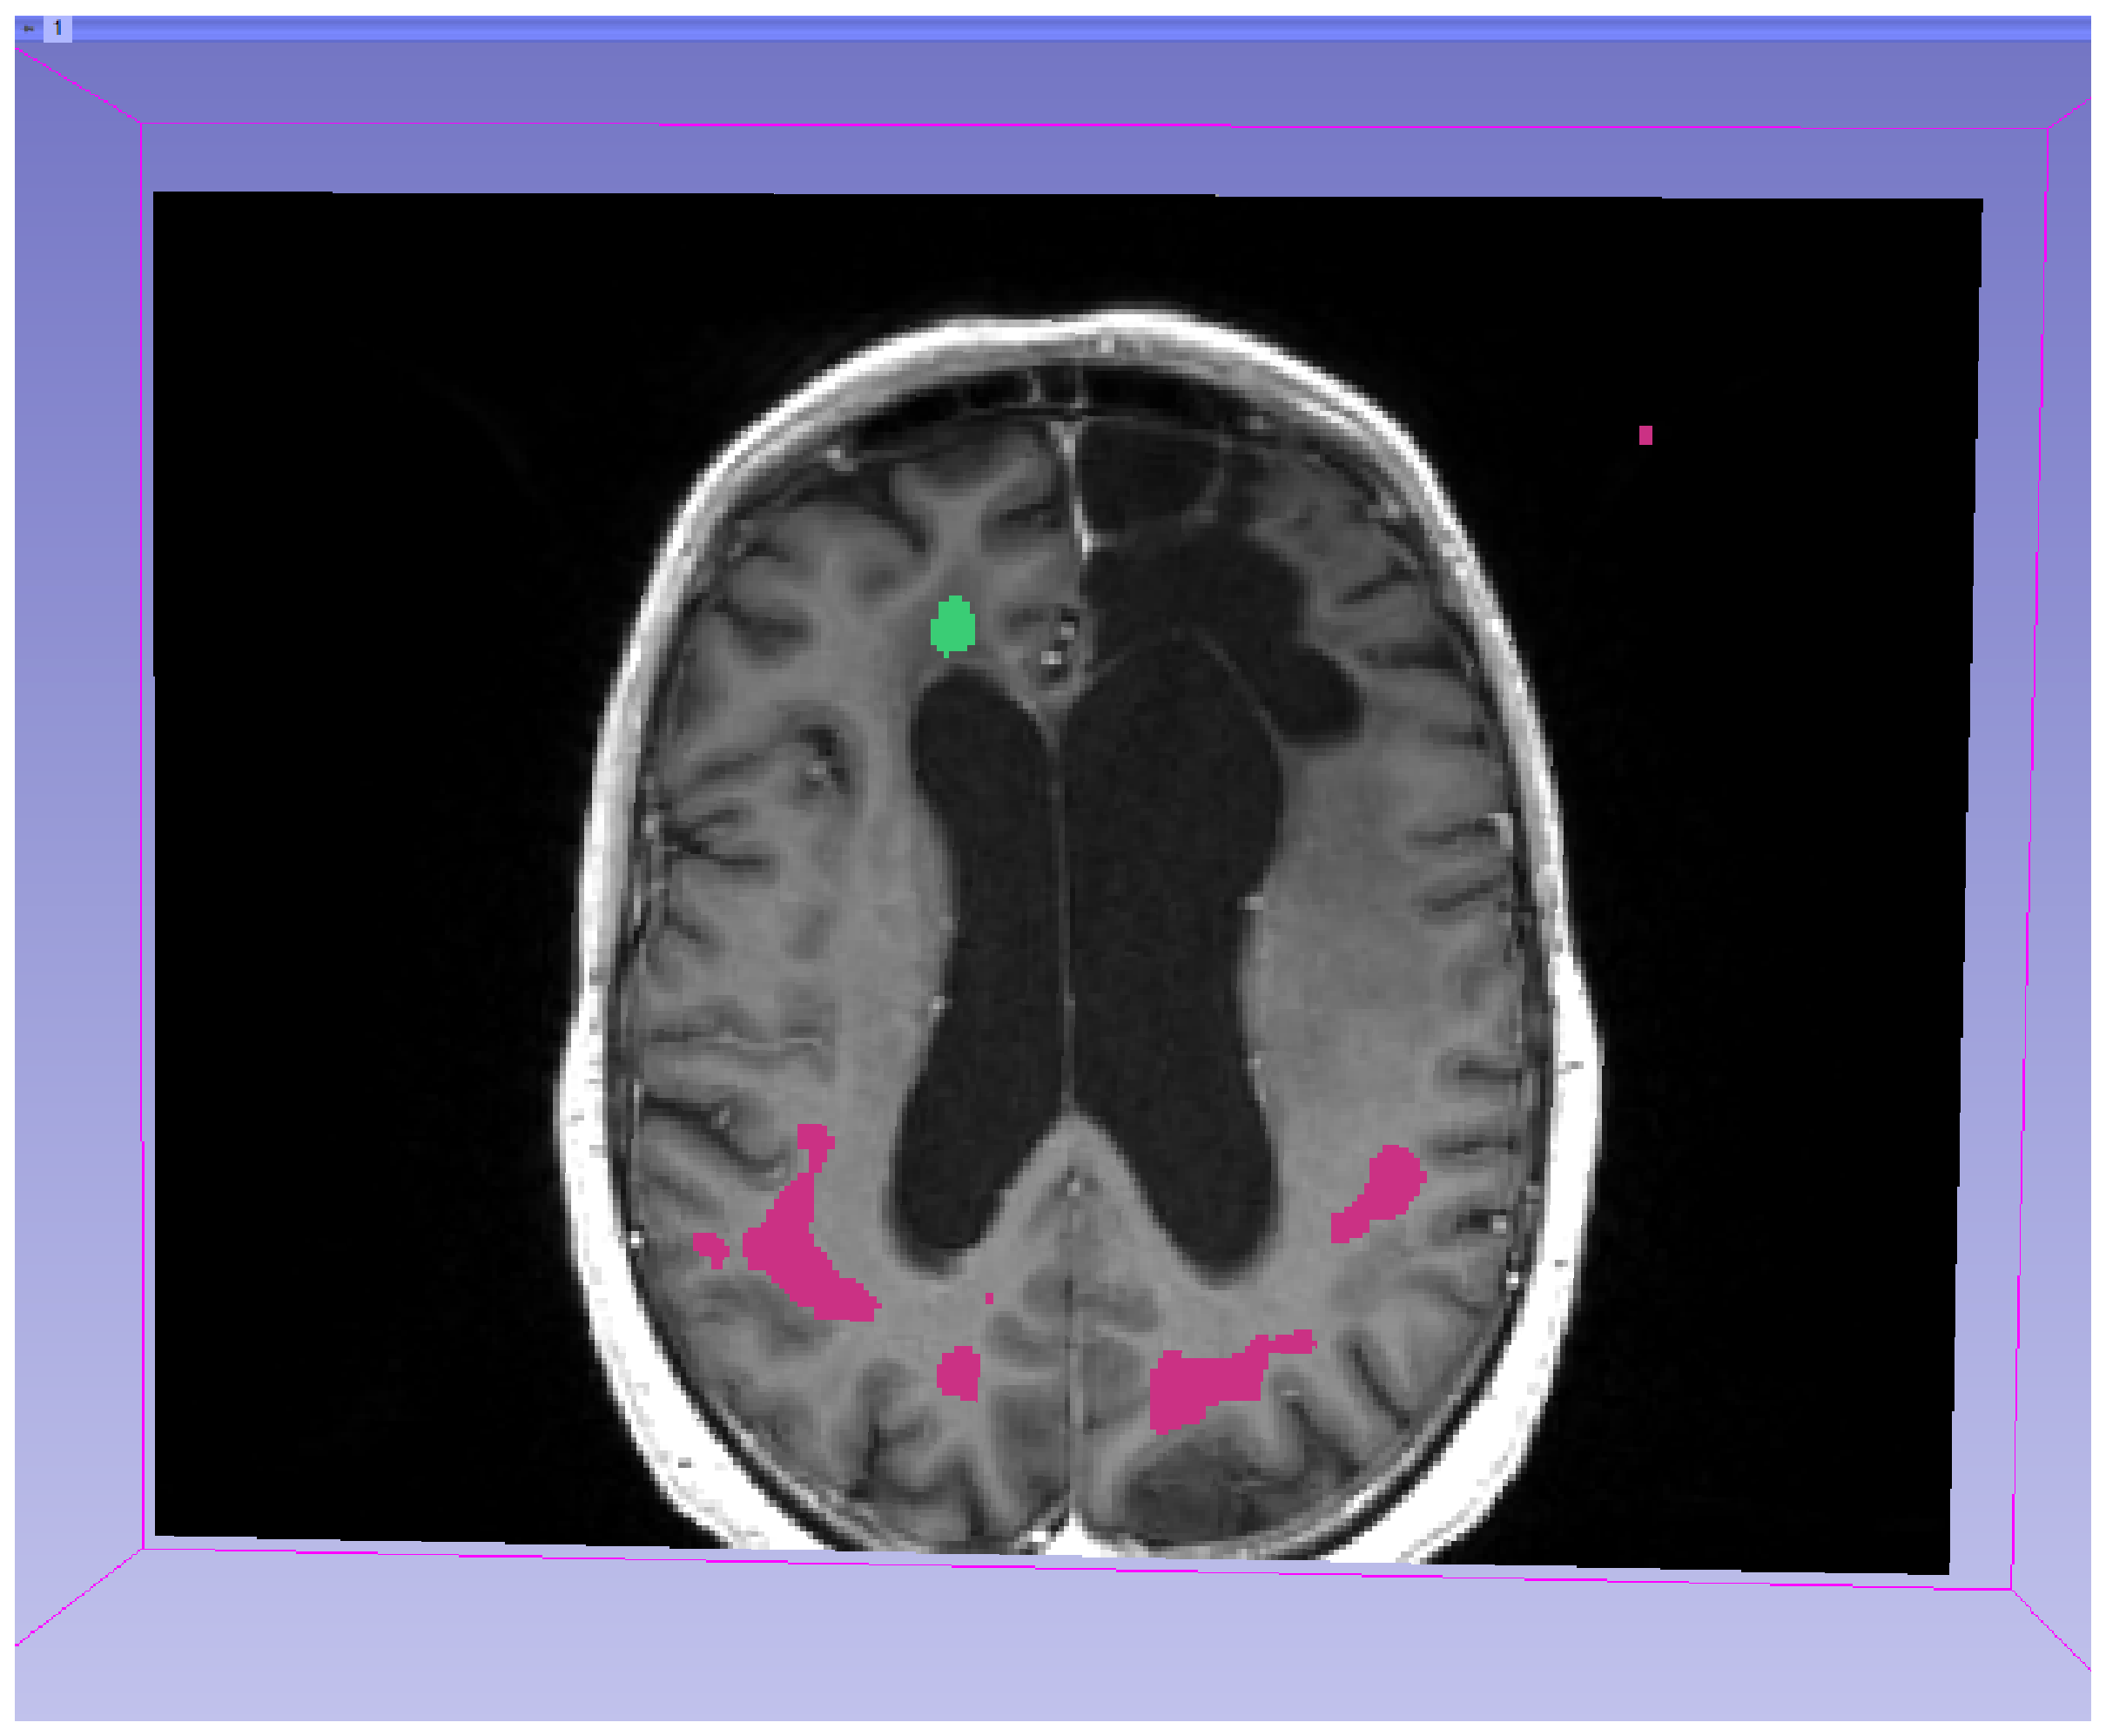
\includegraphics[scale=0.2]{/experiment_B2_P3/B2_Tensor_Traversal1.eps}
  \caption{Tensor-based method. Patient 3: Traversal plane}
  \label{B2_TTraversal1}
\end{figure}

\begin{figure}[H]
  \centering
  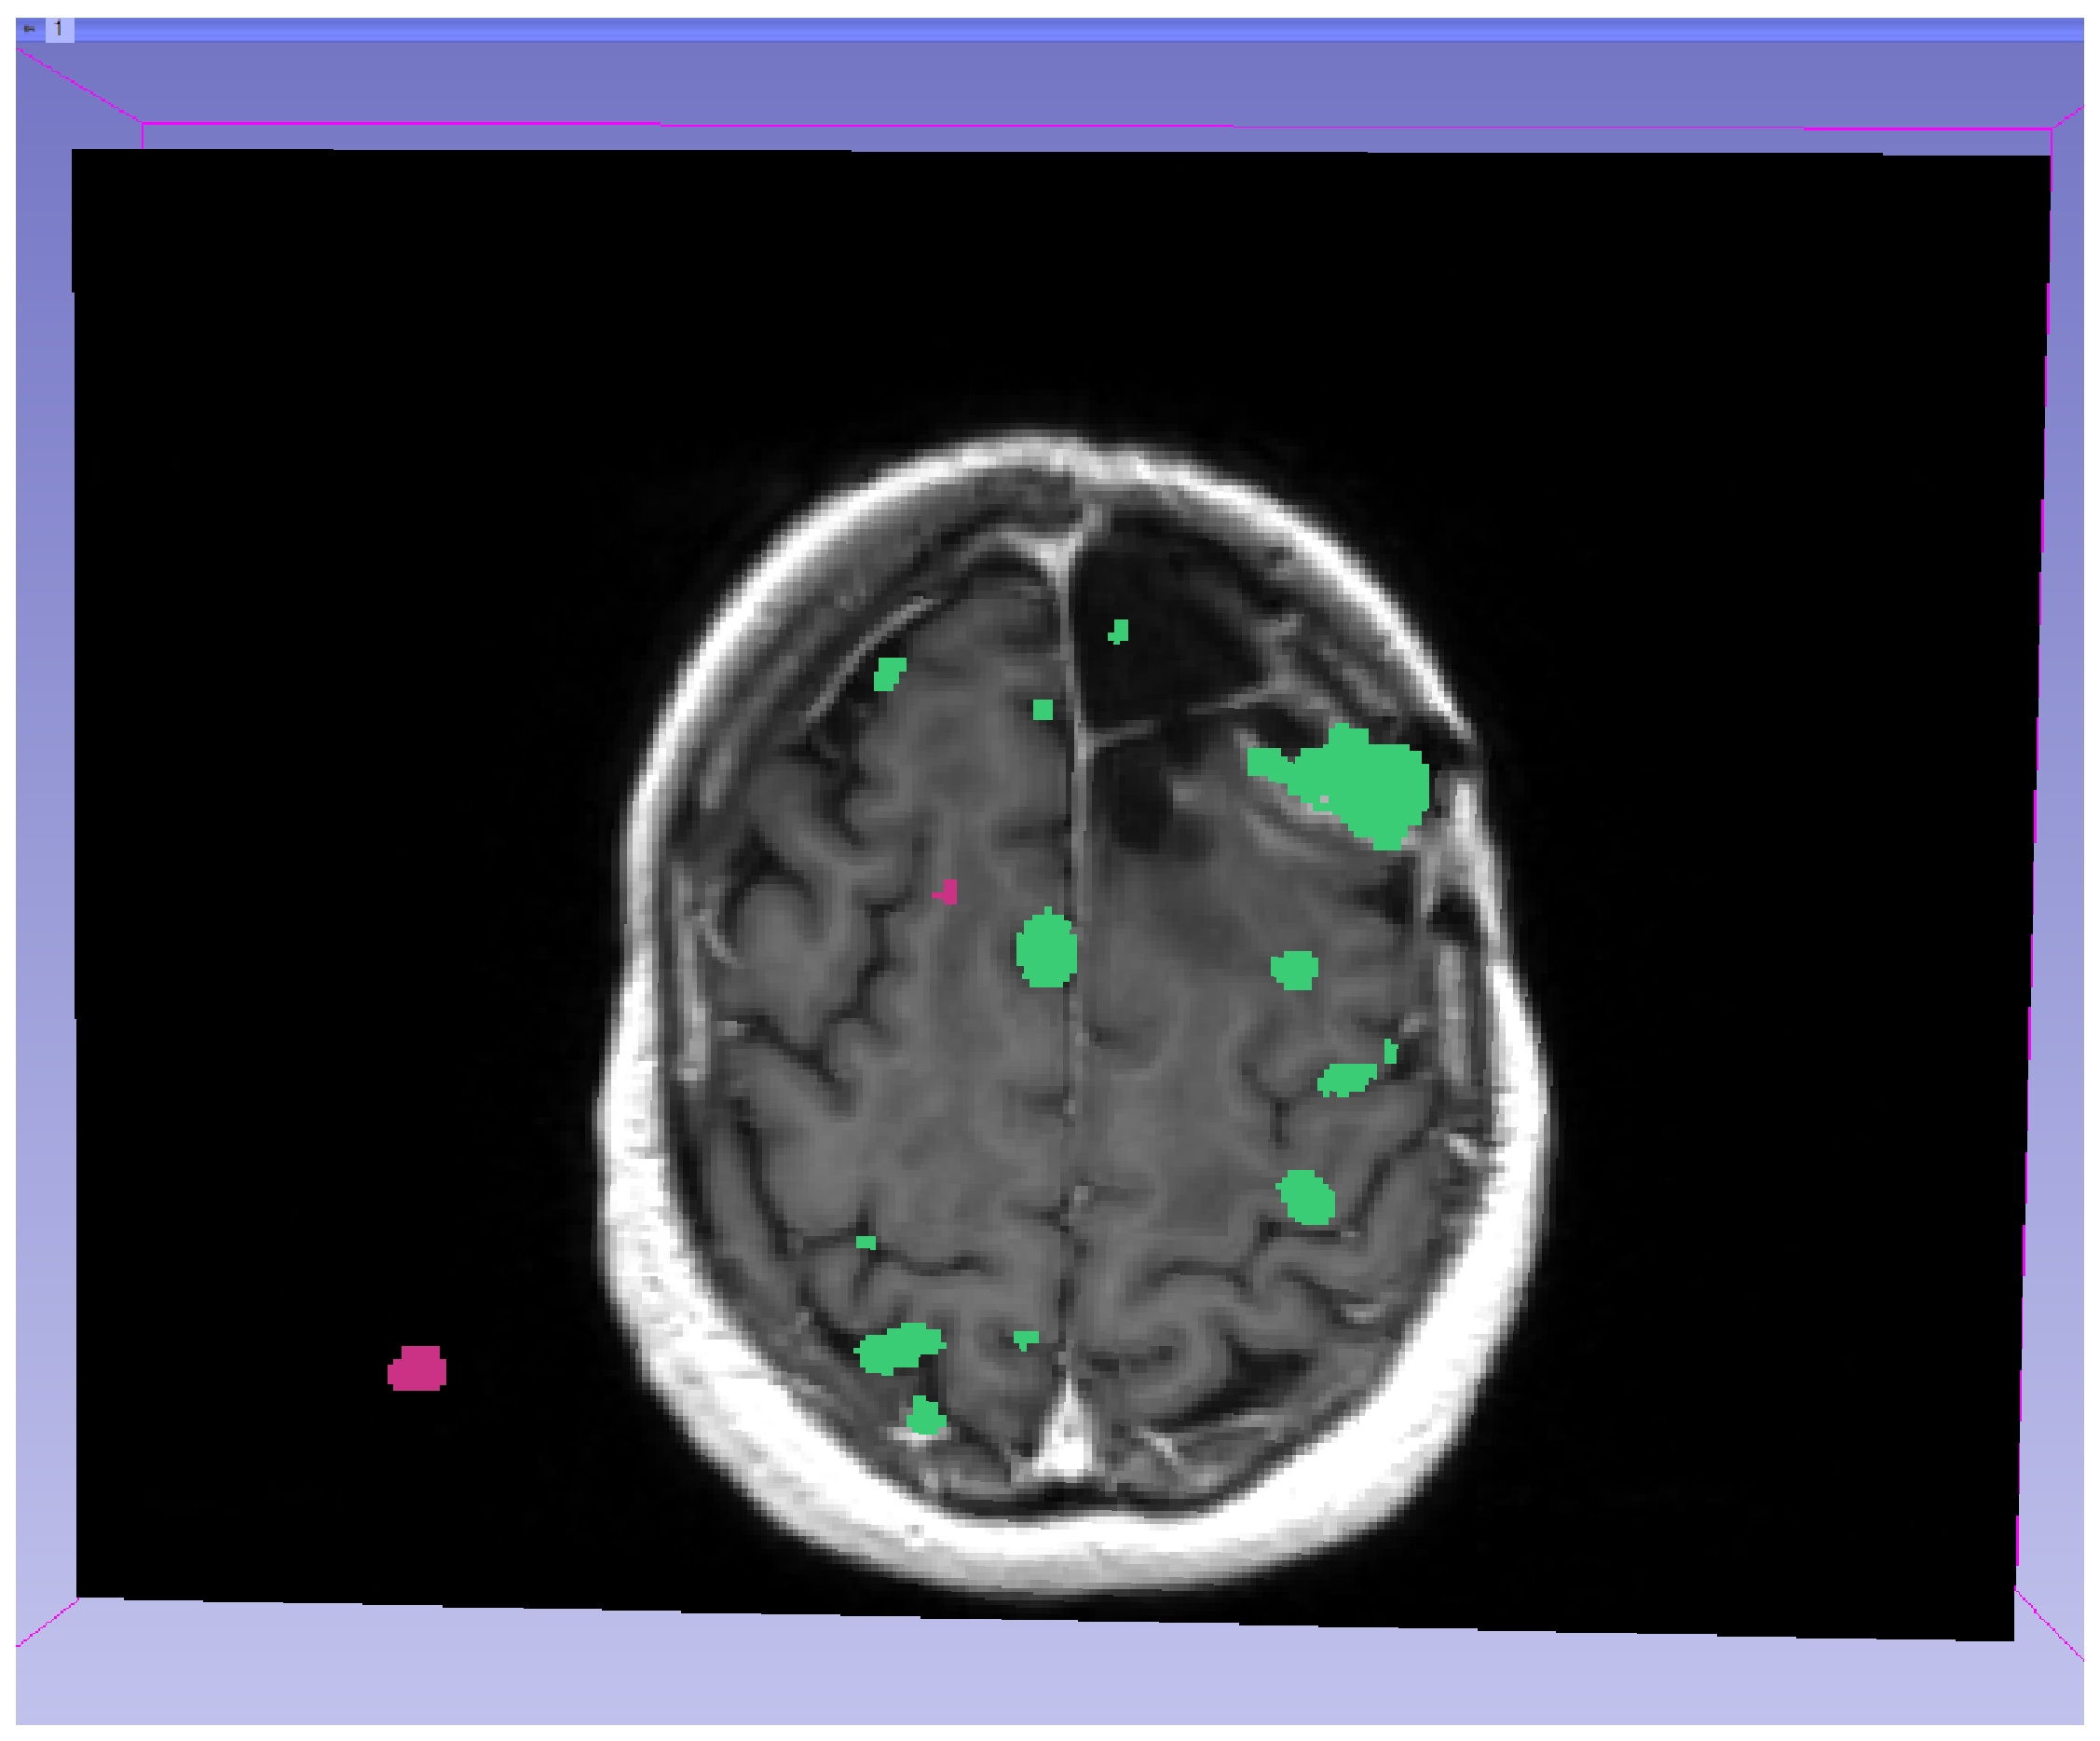
\includegraphics[scale=0.2]{/experiment_B2_P3/B2_Tensor_Traversal2.eps}
  \caption{Tensor-based method. Patient 3: Upper traversal plane}
  \label{B2_TTraversal2}
\end{figure}

\begin{figure}[H]
  \centering
  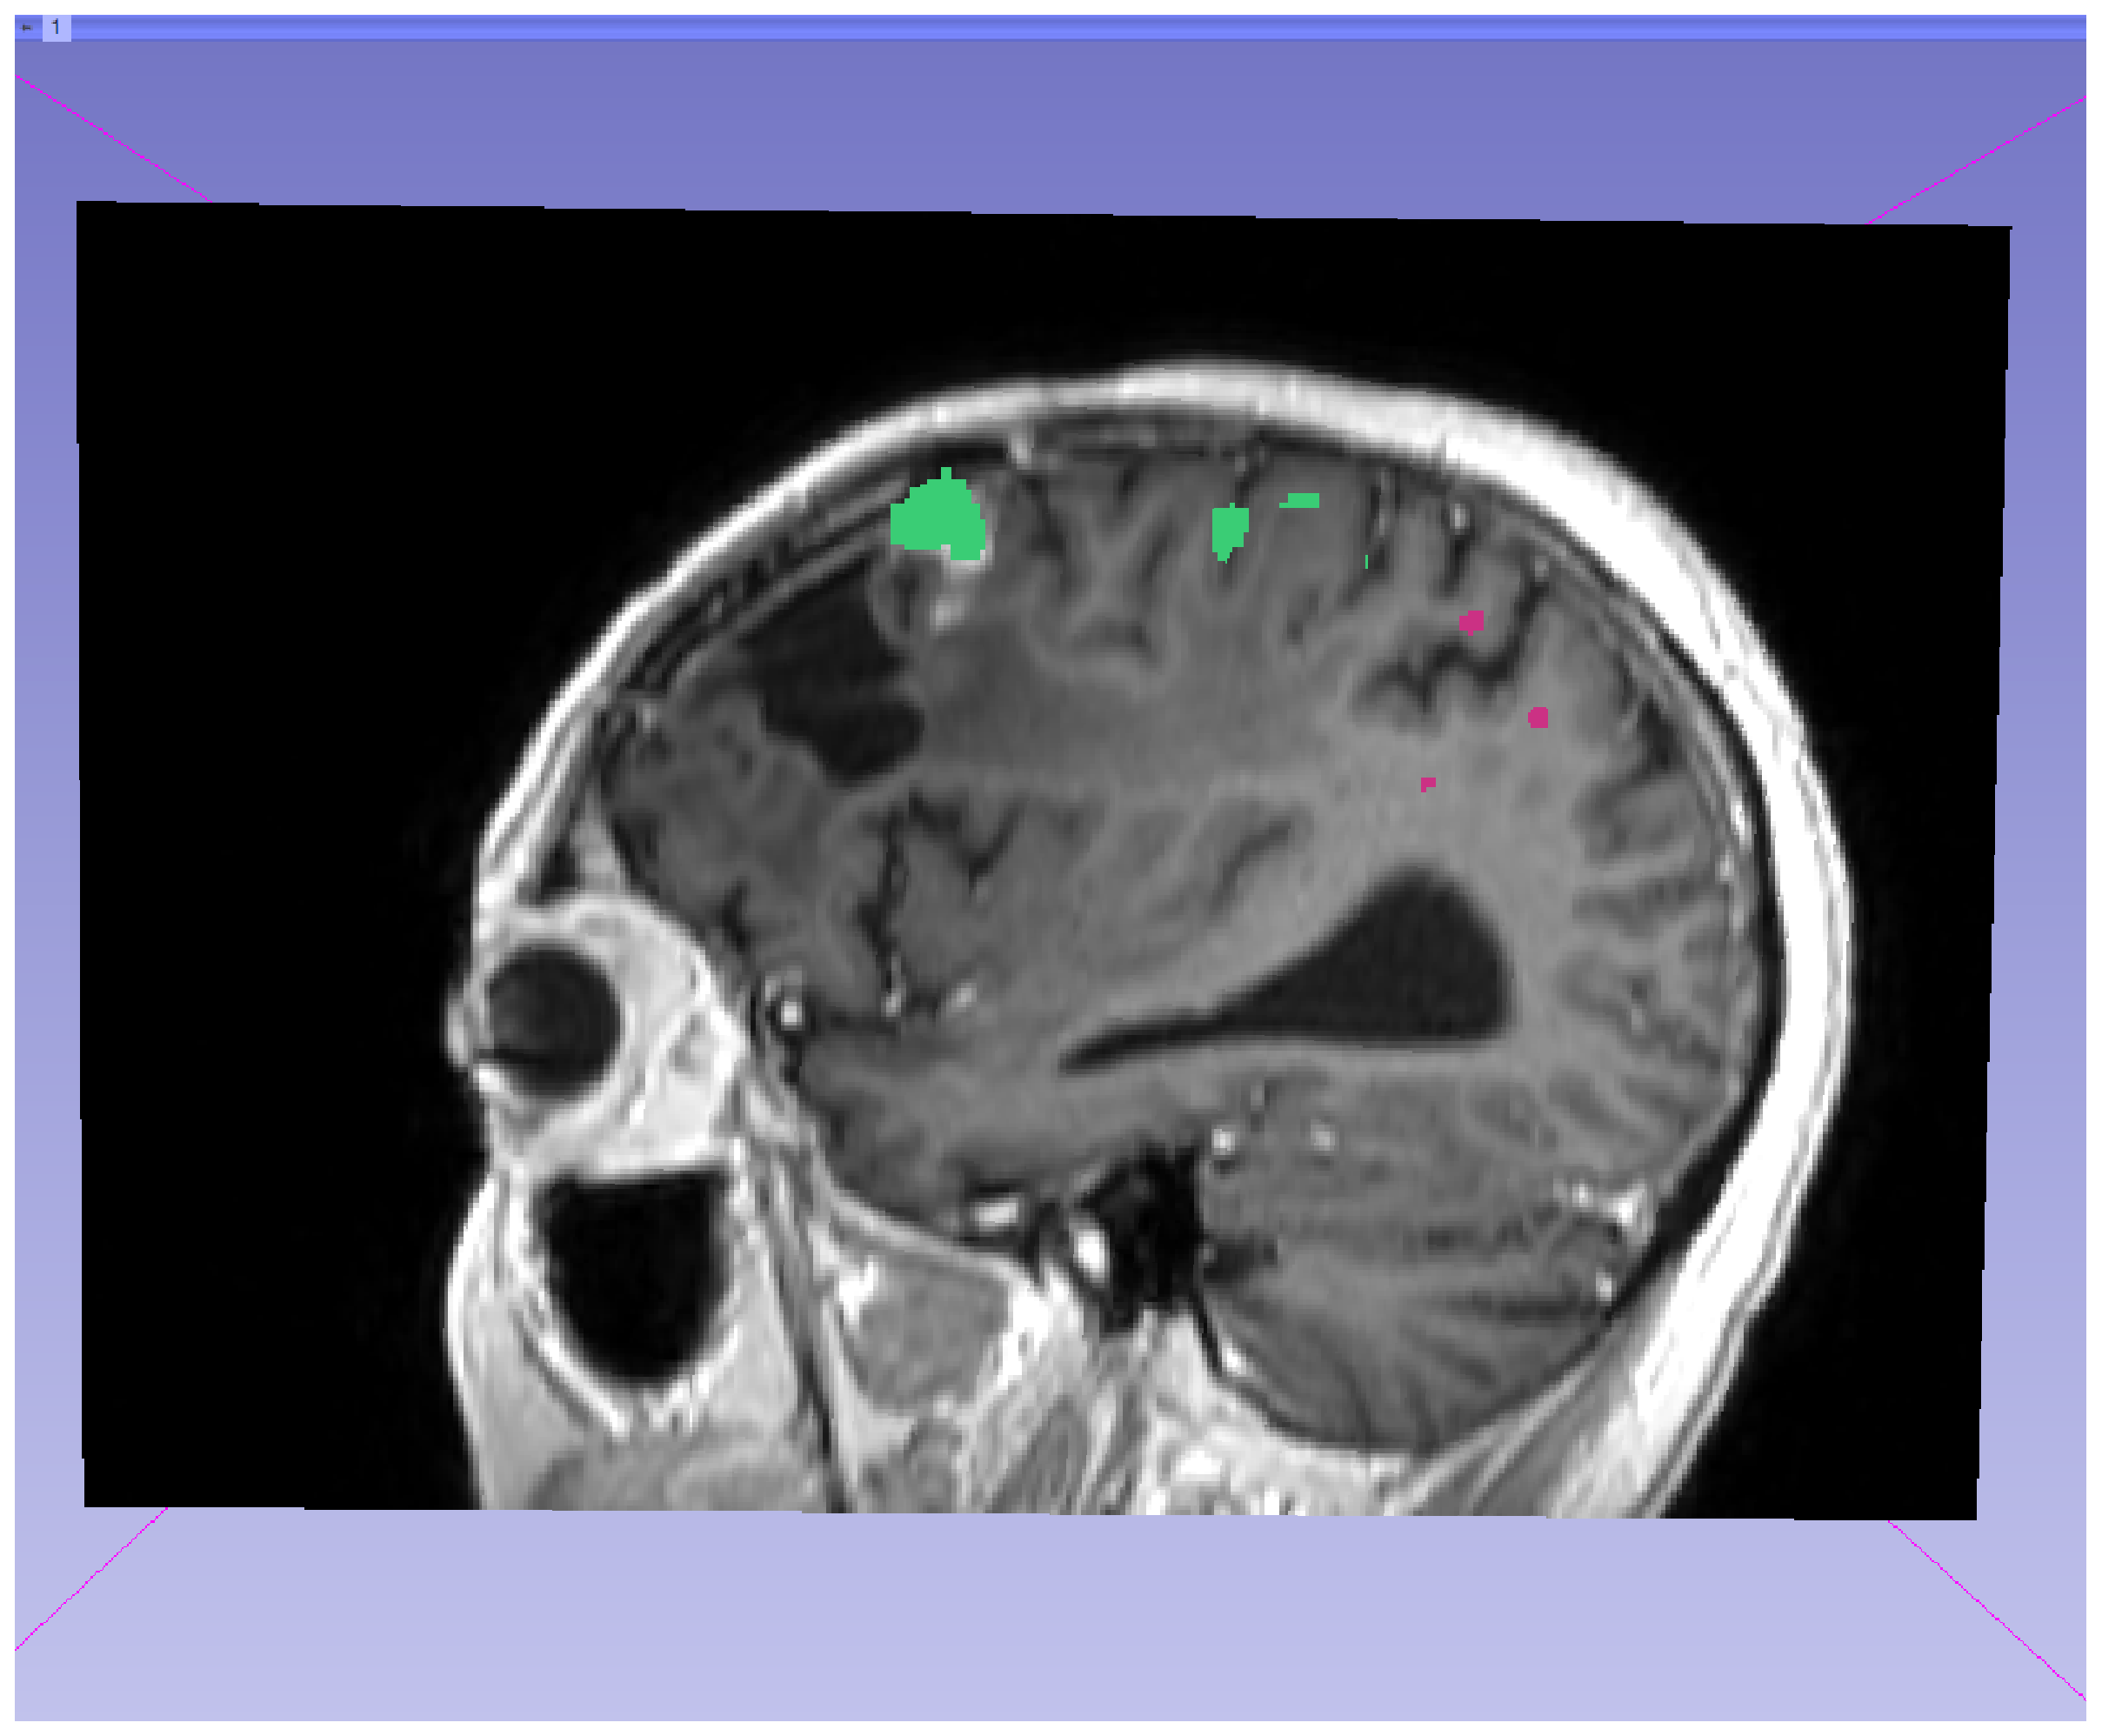
\includegraphics[scale=0.2]{/experiment_B2_P3/B2_Tensor_Sagittal.eps}
  \caption{Tensor-based method. Patient 3: Sagittal plane}
  \label{B2_TSagittal}
\end{figure}